%%%%%%%%%%%%%%%%%%%%%%%%%%%%%%%%%%%%%%%%%
%  Telemac3D Documentation
%  Theory guide
%
%%%%%%%%%%%%%%%%%%%%%%%%%%%%%%%%%%%%%%%%%

%----------------------------------------------------------------------------------------
%	PACKAGES AND OTHER DOCUMENT CONFIGURATIONS
%----------------------------------------------------------------------------------------
\documentclass[Telemac3D]{../../data/TelemacDoc} % Default font size and left-justified equations

%%---------------------------------------------------------------------------
%%Equations
%%---------------------------------------------------------------------------
\renewcommand{\Grad}{\vec \nabla}
\renewcommand{\Div}{\nabla \cdot}
\renewcommand{\Lap}{\nabla^2}%{\text{lap}\hspace{0.1em}}
\newcommand{\BDiv}{\vec{\nabla} \cdot}
\newcommand{\BLap}{\vec{\nabla}^2}
\newcommand{\DivD}{\nabla_{2D} \cdot}
\newcommand{\Divast}{\nabla^* \cdot}

%%---------------------------------------------------------------------------
%% Tableaux
%%---------------------------------------------------------------------------
%\usepackage{booktabs,multirow}
%\usepackage{lscape}
%\usepackage{longtable}
%\newcommand{\minitab}[2][1]{\begin{tabular}{#1}#2\end{tabular}}
%%\usepackage{array}
%%\newcolumntype{L}[1]{>{\raggedright\let\newline\\\arraybackslash\hspace{0pt}}m{#1}}
%%\newcolumntype{C}[1]{>{\centering\let\newline\\\arraybackslash\hspace{0pt}}m{#1}}
%%\newcolumntype{R}[1]{>{\raggedleft\let\newline\\\arraybackslash\hspace{0pt}}m{#1}}

%%---------------------------------------------------------------------------
%% Nomenclature
%%---------------------------------------------------------------------------
\usepackage{ifthen}
\usepackage{nomencl}
%
\makenomenclature
\renewcommand{\nompreamble}{\markboth{%
                            \MakeUppercase\nomname}{\MakeUppercase\nomname}%
                           }

\renewcommand{\nomgroup}[1]{
\ifthenelse{\equal{#1}{C}}{\item[\textbf{In the continuous domain}]}{
\ifthenelse{\equal{#1}{D}}{\item[\textbf{In the discrete domain}]}{
{}
}% matches discrete domain
}% matches continuous domain
}

\begin{document}

\let\cleardoublepage\clearpage
%----------------------------------------------------------------------------------------
%	TITLE PAGE
%----------------------------------------------------------------------------------------
\title{TELEMAC-3D}
\subtitle{Theory guide}
\version{\telmaversion}
\author{}
\date{\today}
\maketitle
\clearpage

%----------------------------------------------------------------------------------------
%	AUTHORS PAGE
%----------------------------------------------------------------------------------------

\newpage

\thispagestyle{empty}

\chapter*{Authors and contributions}
This theory guide was created by Agnès Leroy (EDF R\&D, LNHE), based on the previous available TELEMAC-3D
documentation. In particular, most of the material came from documents written by Jean-Michel
Hervouet (EDF R\&D, LNHE), be it his book, \textit{Hydrodynamics of Free-Surface Flows}, which also lists a number of contributors, or the
TELEMAC-3D release notes. The release notes also included contributions by Chi-Tuân Pham (EDF R\&D, LNHE).
This guide, as well as the abovementioned sources, rely on previous work by Jacek Jankowski and Astrid Decoene during their respective PhD theses.
It also benefits from contributions by Lamia Abbas, Pierrick Quemar, Antoine Joly and Jacques Fontaine.

\newpage

\chapter*{Work under construction}\label{workunderconstruction}
We would like to warn the reader that this document is still under construction and
could be improved in many ways. Any remarks, suggestions, corrections, etc. are welcome
and can be submitted to the TELEMAC developing team through the forum in the Documentation
category: \url{http://www.opentelemac.org/index.php/kunena/10-documentation}.

\newpage

\chapter*{Abstract}\label{Abstract}
This guide aims at providing a comprehensive overlook of the theory behind TELEMAC-3D.
It is based on Jean-Michel Hervouet's book, \textit{Hydrodynamics of Free-Surface Flows} \cite{hervouet007}, as well as
on the previous TELEMAC-3D release notes. It is organised into four chapters: the first two describe the equations
and modelling choices in a continuous framework, as well as the principles of the Finite Elements method.
The latter was nearly directly taken from \textit{Hydrodynamics of Free Surface Flows}, but
also includes some contributions from Jacek Jankowski's PhD thesis.
After this, the time discretisation and then the space-time discretisation of the equations are described in two separate chapters.
While the first two chapters are rather classical, the last two are specific to TELEMAC-3D. They benefitted from a lot
of material from the former release notes and from \textit{Hydrodynamics of Free-Surface Flows}.
They are still unfinished at this stage. In particular, they contain some information regarding the resolution of the advection
in TELEMAC-3D and the treatment of tidal flats, but these two sections directly come from the last release notes
and have not been adapted to this guide yet. Nevertheless, we hope that these chapters will help the
TELEMAC-3D users and developers better understand what is at the core of the module.\\

The main contributions in this theory guide, compared to previous works, lie in the new format
of the document, which aims at gathering all the theoretical background of TELEMAC-3D.
It includes highlighted remarks regarding the limits and possible improvements of the models used in the code.
The chapter 3 is new: it aims at giving the reader an overview of the time scheme, even though all
the demonstrations of consistency, conservation, etc. are only valid when written for the space-time
discretised equations. New notations are adopted compared to previous works, with the hope that
they will facilitate the understanding of the numerical schemes.


%----------------------------------------------------------------------------------------
%	COPYRIGHT PAGE
%----------------------------------------------------------------------------------------

\newpage

\thispagestyle{empty}

\TelemacCopyright{}


%----------------------------------------------------------------------------------------
%	TABLE OF CONTENTS
%----------------------------------------------------------------------------------------


\pagestyle{empty} % No headers

\tableofcontents% Print the table of contents itself

%\cleardoublepage % Forces the first chapter to start on an odd page so it's on the right

\pagestyle{fancy} % Print headers again

%----------------------------------------------------------------------------------------
%	The whole thing
%----------------------------------------------------------------------------------------
%%===========================================================================
%\section{Reminders and definition of variables}
%%===========================================================================
%
%Bold variables will represent vectors and tensors, and plain font will represent scalars; i.e.:
%
%\begin{align}
%\vec{A} = \left[\begin{array}{c}
%		A_x
%		\\
%		A_y
%		\\
%		A_z
%		\end{array}\right]
%\end{align}
%
%Furthermore, the following operators are defined:
%
%\begin{subequations}
%\begin{align}
%\Grad\{A\}		= & \vec{\nabla} A
%\\
%\Grad\{\vec{A}\}		= & \vec{\nabla} \vec{A}^T
%\\
%\Div\{\vec{A}\}	= & \vec{\nabla} \cdot \vec{A}
%\\
%\Lap\{B,A\} =	& \vec{\nabla} \cdot \left( B\vec{\nabla} A\right)
%\notag\\
%			=	& \Div\{B\Grad\{A\}\}
%\\
%\BLap\{B,\vec{A}\} =	& \vec{\nabla} \cdot \left( B\vec{\nabla} \vec{A}^T\right)
%\notag\\
%						=	& \Div\{B\Grad\{\vec{A}\}\}
%\end{align}
%\end{subequations}
%
%Where $\vec{\nabla}$ is the nabla operator defined as:
%
%\begin{align}
%\vec{\nabla} = \left[\begin{array}{c}
%		\dfrac{\partial}{\partial x}
%		\\[1em]
%		\dfrac{\partial}{\partial y}
%		\\[1em]
%		\dfrac{\partial}{\partial z}
%		\end{array}\right]
%\end{align}
%
%In addition $\vec{A}^T$ is the transpose of vector $\vec{A}$.

%===========================================================================
% Nomenclature
%===========================================================================

\printnomenclature

\chapter{Equations and modelling choices in a continuous framework}\label{Chapter1}
\section{Notations and concepts in geometry}

The domain of study $\Omega$ in the referential $R=(O,x,y,z)$ ($Oz$ along the
vertical) is limited below by the bed described by the equation
$z=b(x,y,t)$, or in most situations only $z=b(x,y)$, and above by the
free surface described by the equation $z=\eta(x,y,t)$. It is limited
laterally by vertical lines. Its boundary is $\Gamma$. The projection of
$\Omega$ on the horizontal plane $(O,x,y)$, that will be later our
two-dimensional domain, is denoted by $\Omega_{2D}$ (see the figure \ref{figure1}).
The domain of calculation is thus defined by:%
\begin{equation}
\Omega=\left\{  \left(  x,y,z\right)  \in \mathbb{R}^{3}\text{ such that }\left(
    x,y\right)  \in\Omega_{2D}\,\ \text{and }\,b(x,y,t)\leq z\leq \eta%
  (x,y,t)\right\}
\end{equation}
%
\begin{figure}[H]%
  \centering
  \includegraphics
  [scale=0.4]%
  {graphics/domain_definition.pdf}%
  \caption{Sketch of the calculation domain (inspired by \cite{hervouet007}).}%
  \label{figure1}%
\end{figure}
\begin{CommentBlock}{Remark:}
  At the moment, bed motion is possible only when modelling
  the bed evolution due to sediment transport in TELEMAC-3D. Then, $b$ is really a function of time,
  which modifies the equations presented in this chapter,
  but we did not detail the corresponding changes in the present version of the document.
\end{CommentBlock}

Gravity is directed towards decreasing $z$.
The height of the water column, or water depth, will be denoted by $h$ and is
equal to $\eta-b$.
The bed elevation is given data. The water depth is generally an unknown quantity.
The time will be denoted by $t$. Throughout the document, vectors with the subscript ${2D}$
correspond to the 2D horizontal vector
of $x$ and $y$ components: let $\vec{u}=u \vec{e}_x+v \vec{e}_y+w\vec{e}_z$ be the 3D velocity, then
$\vec{u}_{2D}= u \vec{e}_x+v \vec{e}_y$.\\

Let us now define the normal vectors to the boundaries.
There are four types of boundaries to be considered: the bed $\Gamma_b$,
the free-surface $\Gamma_\eta$, liquid lateral boundaries $\Gamma_l$ and solid
lateral boundaries $\Gamma_s$. Let $\vec{n}$ be the normal to a boundary, oriented outwards the domain.
We denote by $\vec{n}_b$, $\vec{n}_\eta$, $\vec{n}_l$ and $\vec{n}_s$ the outward normal to the bed,
the free-surface, the liquid lateral boundaries and the solid lateral boundaries.
The free surface is a univalent function of coordinates $x$ and $y$, which
excludes calculation of waves on the verge of breaking, and varies with time.
Its equation is in the form of $z=\eta(x,y,t)$. It can also be written as
$\Phi(x,y,z,t)=0$ with:%
\begin{equation}
  \Phi(x,y,z,t)=z-\eta(x,y,t)
\end{equation}
The normal to the free surface, directed towards increasing $z$ (hence
external in relation to the volume containing water), is then the vector (not normalised):%
\begin{equation}
\vec{n}_{\eta}\,=\,\Grad(\Phi)
\end{equation}
This vector has the following components:
\begin{equation}
  \vec{n}_{\eta} =\left(  -\dfrac{\partial \eta}{\partial x},-\dfrac{\partial \eta%
    }{\partial y},1\right)
\end{equation}
The normal to the bed would be expressed in the same way but by replacing
$\eta$ by $b$, and with a minus sign to make it external to the volume of
water. That is:%
\begin{equation}
  \vec{n}_{b}=\left(  \dfrac{\partial b}{\partial x},\dfrac{\partial b%
    }{\partial y},-1\right)
\end{equation}
Note that $\vec{n}_{\eta}$ and $\vec{n}_{b}$ are not defined as unit vectors.
In \telemac{3d}, the bed elevation is a univocal function of coordinates $x$ and $y$.

\begin{CommentBlock}{Possible improvement:}
  The fact that the function $b(x,y)$ is univocal is imposed by the choices in the numerical
  scheme of \telemac{3d}. It implies that vertical sections of the bed can only be
  represented through a steep slope. Investigations regarding how to extend the \telemac{3d}
  software to non univocal beds have been undertaken but are still in progress
  (see \textit{e.g.} \cite{Wang2016}).
\end{CommentBlock}

% ---------------------------------------------------------------------------
\section{The Navier-Stokes equations}
% ---------------------------------------------------------------------------

%%%%%%%%%%%%%%%%%%%%%%%%%%%%%%
%\subsection{Formulation}
The Navier--Stokes equations for incompressible flows consist of two equations: the continuity and the momentum equations.
We first consider a possibly compressible flow in a domain $\Omega$ of dimension 3.
The compressible continuity equation represents the mass conservation in a continuous medium and reads:
\begin{equation}\label{eq:ContinuityRef}
  \dfrac{\partial \rho}{\partial t} + \Div (\rho \vec{u}) = 0
\end{equation}
where $\rho$ is the density, $\vec{u}$ the velocity, $\vec{g}$ is the gravity and $t$ is the time.
The continuous gradient operator is denoted by $\Grad$ and the divergence by $\Div$.
The Navier--Stokes momentum equation is obtained from the Cauchy momentum equation for a continuous medium where a behaviour
law is introduced to model the stress tensor.
We recall the Cauchy equation:
\begin{equation}\label{eq:MomentumRef}
  \dfrac{\partial \vec{u}}{\partial t} + (\vec{u} \cdot \Grad) \vec{u} = \dfrac{1}{\rho}\vec{\Div}\vec{\sigma} + \vec{g} + \vec{F}
\end{equation}
In this equation, $\vec{\sigma}$ is the Cauchy stress tensor, $\vec{F}$ are external forces other than the gravity (\textit{e.g.} the Coriolis and centrifugal forces, see the section \ref{sec:coriolis}).
% Note that equation~\eqref{eq:Cauchy} was written in an Eulerian framework, where the position field $\vec r$ is given by the initial condition $\vec r(t_0) = \vec{r}_0$ with $t_0$ the initial time.
On the other hand, the behaviour law used for a Newtonian fluid reads%
% \footnote{In this work, non-Newtonian fluids are not considered since at this stage
%   the scope of applications of the developed model concerns water or air flows. Though, it is possible to introduce non-Newtonian models in SPH as was done in~\mbox{\cite{Herault-spheric-2011}} for example.}
:
\begin{equation}\label{eq:fluidBehaviour}
  \begin{array}{l}
    \vec{\sigma} = -p \vec{I} + \vec{\sigma}_\tau \medskip \\
    \vec{\sigma}_\tau = \lambda~ \Div \vec{u}~ \vec{I} + 2\mu\vec{s}
  \end{array}
\end{equation}
where $\vec{I}$ is the identity tensor in dimension 3, $\vec{\sigma}_\tau$ is the shear-stress tensor, $\vec{s}$ is the strain-rate tensor,
$p$ is the pressure, $\mu$ is the dynamic molecular viscosity
and $\lambda$ is equal to $\zeta-2/3\mu$ where $\zeta$ is the bulk viscosity.
The tensor $\vec{s}$ is defined as:
\begin{equation}\label{eq:strain-rate}
  \vec{s} = \dfrac{1}{2}\left[\Grad\vec{u} + \Grad\vec{u}^T\right]
\end{equation}
where $~^T$ denotes the transpose of a vector or tensor.
The behaviour law~\eqref{eq:fluidBehaviour} was obtained by introducing a model for viscosity in fluids based on an analogy with a model for particle friction.
%%%%%%%%%%%%%%%%%%%%%%%%%%%%%%

Most of the time, the flows considered here involve buoyancy effects due to active scalars.
Density variations in buoyant flows mainly affect the flow dynamics through the gravity term.
We consider that the Boussinesq approximation is valid for the flows considered here, \textit{i.e.} $\Delta \rho/\rho_0 \ll 1$
where $\rho_0$ is the reference density and $\Delta\rho$ the fluctuations around
it\footnote{The upper limit for the Boussinesq approximation validity is considered in~\cite{Viollet1997} to be $\Delta \rho/\rho < 0.1$.}.
This enables the treatment of buoyancy affecting the fluid motion by means of the gravity term only
(see the section \ref{sec:boussinesq}).
Then, the fluid density is considered as constant and the continuity equation \eqref{eq:ContinuityRef} can be rewritten as:
\begin{equation}
  \Div \vec{u} = 0
  \label{eq:ContinuityFS}
\end{equation}

The equation \eqref{eq:ContinuityFS} can be used to simplify the shear-stress tensor $\vec{\sigma}_\tau$.
Considering that the density $\rho$ is constant, and neglecting the term $\vec{\Div} \left(\mu \Grad \vec{u}^T\right)$,
the Navier--Stokes equations then read:
\begin{equation}\label{eq:NS_buoyant}
  \left\{
    \begin{array}{l}
      \Div \vec{u} = 0 \medskip \\
      \dfrac{\partial \vec{u} }{\partial t} + (\vec{u} \cdot \Grad) \vec{u} = -\dfrac{1}{\rho} \Grad p + \dfrac{1}{\rho} \vec{\Div} \left(\mu \Grad \vec{u}\right)+ \vec{g} + \tilde{\vec{F}}\\
    \end{array}
  \right.
\end{equation}
where $\tilde{\vec{F}}$ represents the external forces plus the buoyancy terms (see the section~\ref{sec:FS-NS},
equation \eqref{eq:buoyancyTerms} for their definition).

\begin{WarningBlock}{Warning:}
  The term $\vec{\Div} \left(\mu \Grad \vec{u}^T\right)$ is always neglected in \telemac{3d}, but it may have an
  influence in case of turbulent flows, when the viscosity is not constant (see the section \ref{turbulence}).
\end{WarningBlock}

% Using the Boussinesq approximation, and the corresponding continuity equation \eqref{eq:ContinuityFS}, then the momentum equation \eqref{eq:MomentumRef} can be rewritten as:
%
% \begin{align}
%   \dfrac{d\vec{u}}{dt} - \BLap\{\nu,\vec{u}\} + \dfrac{1}{\rho}\Grad\{p\} = &
%   \vec{F}+\vec{g}
%   \label{eq:MomentumFS}
% \end{align}
%
% Where $\nu$ is the kinematic viscosity.

% For Nomenclature define name begining with:
% - C for Continuous domain
% - D for Discrete domain
% For example:
\nomenclature[C_rho]{$\rho$}{Fluid density \dotfill (kg/m\textsuperscript{3})}
\nomenclature[C_u]{$\vec{u}$}{Fluid velocity vector \dotfill (m/s)}
\nomenclature[C_u]{$u$}{Fluid velocity along axis $x$ \dotfill (m/s)}
\nomenclature[C_v]{$v$}{Fluid velocity along axis $y$ \dotfill (m/s)}
\nomenclature[C_w]{$w$}{Fluid velocity along axis $z$ \dotfill (m/s)}
\nomenclature[C_F]{$\vec{F}$}{External forces \dotfill (m/s\textsuperscript{2})}
\nomenclature[C_g]{$\vec{g}$}{Acceleration due to gravity \dotfill (m/s\textsuperscript{2})}
\nomenclature[C_p]{$p$}{Fluid pressure \dotfill (kg/m/s\textsuperscript{2})}
\nomenclature[C_nu]{$\nu$}{Kinematic viscosity \dotfill (m\textsuperscript{2}/s)}


% ---------------------------------------------------------------------------
\section{Boundary conditions}
% ---------------------------------------------------------------------------
The closure of the system~\eqref{eq:NS_buoyant} involves the imposition of initial and boundary conditions on the velocity%
\footnote{Note that in fact, with these initial and boundary conditions the existence and uniqueness of a global solution
  to the 3-D Navier--Stokes equations (with any source term and on any time interval)
  was not proved, although it was proved on various particular cases~\cite{Lions1996}.}.
The pressure is the Lagrangian multiplier that stems from the minimisation of the momentum equation
under the constraint \mbox{$\Div \vec{u} = 0$}~\cite{Aris1962}.
Its computation is a key-point in the resolution of the incompressible Navier-Stokes equations.
Many methods were developed to compute it and the strategy adopted in \telemac{3d} is described in the
section~\ref{sec:pressureStrategy}.
It is noteworthy that at this stage of the considerations, the pressure does not require any boundary conditions.

%We also denote by $b(x,y,t)$ the bed elevation and by $\eta(x,y,t)$ the free-surface elevation.\\

\nomenclature[C_Omega]{$\Omega$}{Fluid domain \dotfill (-)}
\nomenclature[C_Gamma_b]{$\Gamma_b$}{Bed boundary of the domain \dotfill (-)}
\nomenclature[C_Gamma_eta]{$\Gamma_\eta$}{Free-surface boundary of the domain \dotfill (-)}
\nomenclature[C_Gamma_l]{$\Gamma_l$}{Liquid boundaries of the domain \dotfill (-)}
\nomenclature[C_Gamma_s]{$\Gamma_s$}{Solid boundaries of the domain \dotfill (-)}
\nomenclature[C_n]{$\vec{n}$}{Normal of the boundary towards the outside of the domain \dotfill (-)}

% ...........................................................................
\subsection{Bed and lateral solid boundaries}\label{sec:solidBoundaries}
% ...........................................................................

On solid boundaries, the kinematic condition expressing the imperviousness is:
\begin{align}
  \left.\vec{u}\right\rvert_{\Gamma_s}\cdot\vec{n}_s = 0\hspace{0.5cm}\text{ and ~} \left.\vec{u}\right\rvert_{\Gamma_b}\cdot\vec{n}_b = 0
  \label{eq:SolidBoundary}
\end{align}
Where $\left.\vec{u}\right\rvert_{\Gamma_i}$ is the fluid velocity on the solid boundary $\Gamma_i$
(either the bed or a lateral boundary).
On the lateral solid boundaries, this is equivalent to:
\begin{align}
  \left.\vec{u}\right\rvert_{\Gamma_s}\cdot\vec{n}_{s2D} = 0\hspace{0.5cm}\text{ on ~}\Gamma_s
  \label{eq:LatSolidBoundary}
\end{align}
since they are vertical.
On the bed, the condition~\eqref{eq:SolidBoundary} is equivalent to:
\nomenclature[C_b]{$b$}{Elevation of the bed \dotfill (m)}
\begin{align}
  % \text{On the bed:\hspace{1cm}}
  \dfrac{d}{dt}(z-b)=0\hspace{0.5cm}\text{ on ~}\Gamma_b
\end{align}
This gives:
\begin{align}
  \left.w\right\rvert_{z=b} - \dfrac{\partial b}{\partial t} - \left.\vec{u}_{2D}\right\rvert_{\Gamma_b}\cdot\Grad_{2D} b = 0\hspace{0.5cm}\text{ on ~}\Gamma_b
  \label{eq:BedBoundary}
\end{align}
Where $\left.w\right\rvert_{z=b}$ is the vertical component of fluid velocity of the bed, $\left.\vec{u}\right\rvert_{\Gamma_b}$ is the fluid velocity on the boundary $\Gamma_b$.
The condition \eqref{eq:BedBoundary} corresponds to the fact that a point of the bed will stay on the bed:
it is a kinematic condition.
%Here, the outwards normal to the bed is calculated as: $\vec{n}_b=-\Grad b$, and since $b$ is only a function of $x$, $y$ and $t$: $\vec{u}\cdot\vec{n}_b=-\vec{u}_{2D}\cdot\Grad_{2D}b$.
On the other hand, the dynamic condition at the solid boundaries accounts for the shear-stress $\vec{\tau}$:
\begin{align}
  \vec{\tau} = -\mu\dfrac{\partial \vec{u}}{\partial\vec{n}}\hspace{0.5cm}\text{ on ~}\Gamma_b \cup \Gamma_s
\end{align}
% \commentAL{To do: write the definition and modelling of the shear-stress.}
The bed shear stress $\vec{\tau}$\index{bed shear stress}
acting on the fluid is oriented opposite to the tangential velocity to the bed:
it is the opposite to the stress applied by the fluid onto the bed, which
is in the direction of the current.
Knowledge of this stress requires knowledge of the flow.
The turbulence models will provide the modelling, based on knowledge of the current in the vicinity of the bed.
In one dimension the shear stress is written as:
\begin{equation}
  \tau=-\rho u_*^{2}%
\end{equation}
which is a definition of a shear velocity $u_{\ast}$.
The shear-stress will then be prescribed as a boundary condition in turbulence models
(see the section \ref{contraintes turbulentes}).

\begin{WarningBlock}{Warning:}
In case no turbulence model is used, the friction is still always prescribed as that of a turbulent flow.
%Do we want to add an option for laminar shear stress?
\end{WarningBlock}
% ...........................................................................
\subsection{Free-surface boundary}
% ...........................................................................

The kinematic condition on the free-surface reads:
\nomenclature[C_eta]{$\eta$}{Elevation of the free-surface \dotfill (m)}
\begin{align}
  \dfrac{d}{dt}(z-\eta)=0 \hspace{0.5cm}\text{ on ~}\Gamma_\eta
\end{align}
As before, this represents the fact that at the free-surface, the velocity of the fluid is equal to the velocity of the free-surface.
If $z$ is on the free surface, this gives:
\begin{align}
  \left.w\right\rvert_{z=\eta} - \dfrac{\partial\eta}{\partial t} - \left.\vec{u}_{2D}\right\rvert_{\Gamma_\eta}\cdot\Grad_{2D}\eta = 0 \hspace{0.5cm}\text{ on ~}\Gamma_\eta
  \label{eq:FreeSurfaceBoundary}
\end{align}
Where $\left.w\right\rvert_{z=\eta}$ is the vertical component of fluid velocity of the free-surface,
$\left.\vec{u}\right\rvert_{\Gamma_\eta}$ is the fluid velocity on the boundary $\Gamma_\eta$.
%Here, the outwards normal of the free-surface is calculated as: $\vec{n}_\eta=\Grad\eta$, and since $\eta$ is only a function of $x$, $y$ and $t$: $\vec{u}\cdot\vec{n}_\eta=\vec{u}_{2D}\cdot\Grad_{2D}\eta$.
On the other hand, the dynamic condition at the free-surface reads:
\begin{align}
  (\vec{\sigma}_\tau \cdot\vec{n}_\eta)_{fluid} = (\vec{\sigma}_\tau \cdot\vec{n}_\eta)_{air}
  \label{eq:dynFS}
\end{align}
Assuming that the pressure is equal to the atmospheric pressure $p_{atm}$ and the viscous air
stress is small enough to be disregarded (which is not the case when wind effects are taken into account),
the condition \eqref{eq:dynFS} comes to:
\begin{align}
  p = p_{atm} \hspace{0.3cm}\text{and}\hspace{0.3cm} \vec{\sigma}\cdot\vec{n}_\eta = 0 \hspace{0.5cm}\text{ on ~}\Gamma_\eta
\end{align}

\subsubsection{Wind-induced stress on the free-surface}
In case the influence of wind is taken into account, wind
forcing appears in the equations through the two-dimensional condition at the surface:
\begin{equation}\label{eq:windstress}
  \vec{\sigma}\cdot\vec{n}_\eta = \mu\dfrac{\partial\vec{u}_{2D}}{\partial n}=\rho_{air}%\dfrac{\rho_{air}}{\rho_{fluid}}
  a_{wind} u_{wind}\vec{u}_{wind}
\end{equation}
$\rho_{air}$, the air density, is a function of the air temperature.
However, in TELEMAC-3D a constant value of 1.3 kg/m$^{3}$ is used for the wind-induced friction
on the free-surface.
$\vec{u}_{2D}$ is the horizontal velocity at the surface and
$\vec{u}_{wind}$ the wind velocity, usually measured 10 m above the water, and $u_{wind}$ is its norm.
The coefficient $a_{wind}$ (dimensionless) is given by Flather \cite{flather76}:%
\begin{equation}%
  \left\{
    \begin{tabular}
      [c]{ll}%
      $a_{wind}=0.565\;10^{-3}\quad$ & if$\quad\left\Vert \vec{w}\right\Vert \leq 5\;$m/s\\
      $a_{wind}=\left(-0.12+0.137\left\Vert \vec{w}\right\Vert\right)\;10^{-3}\quad$ & if $\quad5\,\,$
      m/s$\leq\left\Vert \vec{w}\right\Vert \leq19.22\;$m/s\\
      $a_{wind}=2.513\;10^{-3}\quad$ & if$\quad\left\Vert \vec{w}\right\Vert\geq19.22\;$m/s
    \end{tabular}
  \right.
\end{equation}
The coefficient $a_{wind}$ hides complex phenomena and the above values are
only a guideline. In fact, the influence of the wind depends on the roughness
of the free surface, which is itself dependent on the wind and the distance
over which it is applied (called \textquotedblleft fetch\textquotedblright)%
\index{fetch}%
.
% ...........................................................................
\subsection{Liquid boundaries}
% ...........................................................................

On the open boundaries, additional information is required on the pressure,
the water depth, the velocity, the discharge, etc. These boundaries, which are
purely artificial, usually cause difficulties in numerical modelling.
In particular, certain choices of boundary conditions will not
necessarily lead to well-defined problems (that depends on the nature
of the flow -- sub-critical / super-critical, and its direction).
In \telemac{3d}, the most common ways to prescribe open boundaries are:
\begin{itemize}
\item to prescribe a water level by imposing a hydrostatic pressure profile along the vertical;
\item to prescribe a discharge by imposing a constant horizontal velocity profile along the vertical;
\item to prescribe tidal boundary conditions (see the paragraph below: the horizontal velocities and/or water level are prescribed);
\item to prescribe the scalars values.
\end{itemize}
When the open boundary is experiencing an incoming mass flux, the values specified by the user
for the flow rate, water height or scalars are prescribed. When it is experiencing an outgoing
mass flux, a homogeneous Neumann boundary condition is applied by interpolating the fields based
on the interior values.

It is possible to program more complex open boundary conditions in a dedicated subroutine.
In general, what is to be prescribed onto an open boundary is highly dependent on the flow itself.

\begin{CommentBlock}{Remark:}
At the moment in \telemac{3d} it is not possible to prescribe the dynamic pressure at an open
boundary -- it did not prove necessary until now for the targeted applications.
\end{CommentBlock}


\subsubsection{Tidal boundary conditions}\label{tides}

The theory used to model tides in TELEMAC can be read in \cite{jmj} and
\cite{schureman71}. It is partly described here. When modelling tides, open
boundary conditions for water depth and/or horizontal components of velocity
can vary spatially and temporally and can be calculated at each time step for
every boundary node as a sum of harmonic constituents.

For each harmonic constituent, the water depth $h$ and horizontal components
of velocity $u$ and $v$ are calculated as below, at point $\vec{x}$ and time $t$:
\begin{equation}
f(\vec{x},t) = \sum_{i} f_{i}(\vec{x},t)
\end{equation}
with:
\begin{equation}
f_{i}(\vec{x},t) = f_{i}(t) A_{f_{i}}(\vec{x}) \cos\left(  2\pi\dfrac{t}{T_{i}} -
\phi_{f_{i}}(\vec{x}) + \phi_{i}^{0} + g_{i}(t)\right)
\end{equation}
where $f$ is the water depth $h$ or one of the horizontal components of
velocity $u$ or $v$, $i$ refers to the considered constituent, $T_{i}$ is the
period of the constituent, $A_{f_{i}}$ is the amplitude of the water depth or
one of the horizontal components of velocity of the constituent, $\phi_{f_{i}}$
is the phase, $f_{i}(t)$ and $g_{i}(t)$ are the nodal factors (see below)
and $\phi_{i}^{0}$ is the phase at the original time of the simulation.

\begin{CommentBlock}{Remark:}
In previous versions of \telemac{3d} release notes and in the TELEMAC-2D documentation, different notations were used
for the initial phase and nodal factors. To avoid confusions in the notations,
they are slightly different in the present document: $v_{i}$ (from previous notations)
is denoted here by $g_{i}$ and $u_{i}^{0}$ is denoted by $\phi_{i}^{0}$.
\end{CommentBlock}

The water depth and velocities of each constituent are then summed to obtain water
depths and velocities to prescribe at open boundary conditions:
\begin{equation}
h = \sum_{i} h_{i} - b + z_{mean}
\end{equation}
\begin{equation}
u = \sum_{i} u_{i}
\end{equation}
\begin{equation}
v = \sum_{i} v_{i}
\end{equation}
where $z_{mean}$ is the level used to
calibrate the sea levels. The coefficients $A_{f_{i}}$ and $\phi_{f_{i}}$ are
constant in time and only depend on the location. This information is highly
sought after in the modelling of tides and some databases do exist for
different areas.
Among the different databases of harmonic constants available, four of them
can be used with the TELEMAC system to force the open boundary conditions:

\begin{itemize}
\item Jean-Marc Janin (JMJ) and Xavier Blanchard's model of the English
Channel and the near Atlantic Ocean including the Continental Shelf (4
harmonic constituents) \cite{jmj},

\item LEGOS atlases such as the regional NEA (North East Atlantic) atlas
processed by NOVELTIS/LEGOS in the frame of the COMAPI project funded by CNES
\cite{pairaud1}, \cite{pairaud2} \cite{legos} which covers an area from
Mauritania to the south of Norway (15 or 47 harmonic constituents if the
solution is assimilated with satellite observations or not - the pure
hydrodynamic solution has been modelled with T-UGOm finite element software)
or the global atlas FES,

\item TPXO global tidal solution and regional/local tidal solutions from OSU
(Oregon State University) \cite{osu}, such as the Atlantic Ocean and the
European Shelf (around 11 harmonic constituents depending on the area) or
areas all over the world,

\item PREVIMER atlases with 7 embedded atlases covering the North East
Atlantic (3 different resolutions) with 17 or 38 harmonic constituents.
\end{itemize}

The different databases provide amplitudes and phases for the tidal elevation
and for the two horizontal components of the current most of the time for most
of them. \newline

The nodal factors ($f_{i}(t)$, $g_{i}(t))$ and the phase at the original time
of the simulation ($\phi_{i}^{0}$) are to be taken into account to correct the
slow variations induced by the tilting of the the moon orbit on the Equator.
For solar waves such as S2, there is no correction ($f_{i}(t)$ = 1 and
$g_{i}(t) = \phi_{i}^{0}$ = 0 every time). On the contrary, for lunar waves or
combined waves with at least one lunar wave, these factors have to be
calculated, for example with the formulae coming from Schureman
\cite{schureman71} or Pugh \cite{pugh}. These formulae need the computation of
some previous parameters (mean longitude of moon, mean longitude of sun,
longitude of the lunar perigee, longitude of lunar ascending node).

Three calibration parameters are available for adjusting the results when
calculating tidal open boundary conditions.

\begin{itemize}
\item one multiplier coefficient to calibrate tidal ranges ($CTIDE$),
\item one multiplier coefficient to calibrate velocities ($CTIDEV$),
\item one multiplier coefficient to calibrate sea level ($MSL$).
\end{itemize}

In practise, the previous formulae become:
\begin{equation}
h = CTIDE \sum_{i} h_{i} - b + MSL
\end{equation}
\begin{equation}
u = CTIDEV \sum_{i} u_{i}
\end{equation}
\begin{equation}
v = CTIDEV \sum_{i} v_{i}
\end{equation}
For more information, the reader can read \cite{phammareev6p2} and
\cite{phamlyard}.


\subsubsection{Thompson formulation for radiative open boundary conditions}\label{thompson}

The existence of artificial boundaries in the calculation domains, \textit{e.g.}
in the open sea, often raises the question of boundary conditions and
leads to ill-posed problems. In the open sea, generally only the free-surface
elevation is known. It is tempting to adopt a condition with
imposed elevation and free velocity. When the current is directed
inwards on these boundaries, the problem is ill-posed
and the solution could diverge. The theory of characteristics in one dimension,
which would help to emphasise the required conditions, cannot be applied
strictly in two dimensions. The characteristic curves highlighted
in one dimension are transformed into surfaces (see \cite{daubert67}). The ``radiation''
boundary conditions use the theory of characteristics with a few assumptions.
In particular, this is the case for the Thompson method \cite{thompson}.
In practise, the following approach is used:
\begin{itemize}
\item all the available data at the open boundaries (elevation and velocities)
  are provided and declared as imposed values;
\item the local conditions at the boundaries are studied in the light of the theory of characteristics
  and the Riemann invariants, to determine which information is really necessary
  and which should be kept aside. The new elevations and velocities to be imposed are deduced.
  These are not necessarily the ones provided by the user.
\end{itemize}
The Thompson method, adapted to the shallow water equations, is detailed
in the Appendix A (\ref{appendixA}), but a quick description is given here.
The idea of the Thompson method is to consider the shallow water equations
in matricial form and to change referential so as to
place oneself in a referential local to a boundary point.

\begin{WarningBlock}{Important:}
Since the Thompson formulation is based on the shallow water equations,
it is adapted to flows which are quasi-horizontal close to the open boundaries
(\textit{i.e.} the vertical velocity is about zero in these areas).
When this is not the case, using the Thompson formulation may lead to inconsistencies
(\textit{e.g.} increased numerical dissipation, spurious velocity fields, etc.).
\end{WarningBlock}

Let $(\xi, \zeta)$ be the coordinates in this new referential.
It is then possible to re-write the shallow water system in this referential,
and to derive the following system (see \cite{hervouet007}, pp. 105--108):
\begin{equation}
\dfrac{\partial W}{\partial t} + \Lambda \dfrac{\partial W}{\partial \xi} = LS_\xi
\end{equation}
where $W$ is defined by $dW=LdF$, with:
\begin{equation}
F=\left(\begin{array}{c}h \\ hU \\ hV\end{array}\right), ~~
L=\left(\begin{array}{ccc}
U_\zeta & \dfrac{\partial \xi}{\partial y} & -\dfrac{\partial \xi}{\partial x}\smallskip\\
c-U_\xi & \dfrac{\partial \xi}{\partial x} & \dfrac{\partial \xi}{\partial y}\smallskip\\
c+U_\xi & -\dfrac{\partial \xi}{\partial x} & -\dfrac{\partial \xi}{\partial y}
\end{array}\right)
\end{equation}
On the other hand, $\Lambda$ is defined by:
\begin{equation}
\Lambda=\left(\begin{array}{ccc}U_\xi & 0 & 0 \smallskip \\
0 & U_\xi+c & 0 \\ 0 & 0 & U_\xi-c\end{array}\right)
\end{equation}
with $c=\sqrt{gh}$. Thompson then proposes to consider that $L$ is constant in the
vicinity of a boundary point, and to write $W=\overline{L}F$, with $\overline{L}$ defined by:
\begin{equation}
\overline{L}=\left(\begin{array}{ccc}
\overline{U_\zeta} & \dfrac{\partial \xi}{\partial y} & -\dfrac{\partial \xi}{\partial x}\smallskip\\
\overline{c}-\overline{U_\xi} & \dfrac{\partial \xi}{\partial x} & \dfrac{\partial \xi}{\partial y}\smallskip\\
\overline{c}+\overline{U_\xi} & -\dfrac{\partial \xi}{\partial x} & -\dfrac{\partial \xi}{\partial y}
\end{array}\right)
\end{equation}
where the over-line means that the field is taken as constant.
The Riemann invariants of the vector $W$ are then:
\begin{equation}
\left\{\begin{array}{ll}
W_1 = -h\left(U_\zeta - \overline{U_\zeta} \right) & \text{(advection with velocity $U_\xi$)}\medskip\\
W_2 = h\left(\overline{c}+U_\xi-\overline{U_\xi} \right) & \text{(advection with velocity $U_\xi+c$)}\medskip\\
W_3 = h\left(-\overline{c}+U_\xi-\overline{U_\xi} \right) & \text{(advection with velocity $U_\xi-c$)}
\end{array}\right.
\end{equation}
The method of characteristics is then used to propagate the invariants.
Source terms, if any, are taken into account in a fractional step.
Three (or more, with scalars) characteristic curves per open boundary point thus have to be
calculated. %and, each time the corresponding advection field prepared on the entire domain.
This makes this method more time consuming than only prescribing the field
values at the boundary, but it sometimes is the only way to stabilise a simulation.
Once the Riemann invariants are known, the shallow water variables ($h$, $U$, $V$, $T$) are recovered
with the following formulae:
\begin{equation}
\left\{\begin{array}{l}
h=\dfrac{W_1-W_3}{2\overline{c}} \medskip \\
U = \dfrac{(\partial \xi/\partial y)W_1+(\partial \xi/\partial x)W_2-(\partial \xi/\partial x)h\overline{c}}{h}+\overline{U} \medskip \\
V = \dfrac{(\partial \xi/\partial y)W_2-(\partial \xi/\partial x)W_1-(\partial \xi/\partial y)h\overline{c}}{h}+\overline{V} \medskip \\
T=-\dfrac{W_4}{h}+\overline{T}
\end{array}\right.
\end{equation}

The choice of the local referential system is very important.
In the original method by Thompson,
the normal and tangent to the boundary were used for the referential.
However, in this case characteristics of the same
family stemming from two different points may cross because they have a
different original direction.
In the TELEMAC system,
it was chosen to use the direction of the velocity field itself.\\
\begin{CommentBlock}{Remark:}
An important consequence of this choice is that the velocity $\overline{U}%
_{\zeta }$ is always 0 by definition, which would lead to $W_{1}=0$. This is
true in fact only if we consider that the direction of the referential
changes along characteristics. It is false if we keep the original direction,
which would be consistent with the assumption of constant fields close to the boundary point,
leading to $\overline{L}$. Tests show that it is better to consider that $%
U_{\zeta }$ is indeed not 0, thus sticking to the assumption of constant fields. A
possibility that remains to be tested would be to consider that $U_{\zeta }$
is indeed 0, and taking the norm of the velocity for the component $U_{\xi }$.
\end{CommentBlock}

%\begin{WarningBlock}{Question by Agnès:}
%Le vecteur $\vec{t}$ n'est donc pas coplanaire avec la frontière...
%Est-ce que ce n'est pas un problème ?
%\end{WarningBlock}

In case the velocity is zero at the boundary, the vector $(-g,\Grad\eta)$ is chosen
for the direction. It is indeed the driving term in the momentum equation
that will induce a velocity at the next time step. In this way, water level
gradients are taken into account in the computation of the boundary fields values.
For more details about the implementation, see \cite{hervouet007} pp.105--108
and the release notes for TELEMAC version 6.1 \cite{release61}.

% ---------------------------------------------------------------------------
\section{Treatment of the pressure field in \telemac{3d}}\label{sec:pressureStrategy}

\subsection{Decomposition of the pressure}

In \telemac{3d} the pressure is decomposed into a hydrostatic and a dynamic part, \textit{i.e.}:

\begin{align}
  p=p_h+p_d
\end{align}
Where $p_h$ represents the hydrostatic pressure and $p_d$ the dynamic pressure.

\nomenclature[C_p_h]{$p_h$}{Hydrostatic pressure \dotfill (kg/m/s\textsuperscript{2})}
\nomenclature[C_p_d]{$p_d$}{Dynamic pressure  \dotfill (kg/m/s\textsuperscript{2})}

The hydrostatic pressure is defined by the following equation:
\begin{align}
  p_h = \rho g (\eta-z) + p_{atm}
\end{align}

Under the Boussinesq approximation, this gives:

\begin{align}
  p_h  = g\rho_0(\eta-z) + p_{atm} + g\rho_0\int_z^\eta\dfrac{\Delta\rho}{\rho_0}~dz
\end{align}

The hydrostatic pressure is thus a function of the free-surface elevation $\eta$, and it is necessary to compute the latter.
This is done by solving an equation on $\eta$ that is obtained from the integration of the continuity equation on the vertical.
The derivation of this equation is described in the subsection~\ref{sec:FSequation}.
On the other hand, the dynamic pressure is still coupled to the velocity field, and the strategy adopted in \telemac{3d}
is to compute it using the Chorin and Temam projection scheme~\cite{Chorin1968, Temam1968}.
This is described in the subsection~\ref{sec:Chorin}.
Let us now focus on the computation of the hydrostatic pressure, and so on the computation of the free-surface elevation.


\subsection{The free-surface equation -- solving for the hydrostatic pressure}\label{sec:FSequation}
% ---------------------------------------------------------------------------

It is possible to show that if the continuity equation \eqref{eq:ContinuityFS} and the kinematic condition on the bed~\eqref{eq:BedBoundary} are satisfied,
then the kinematic condition at the free-surface~\eqref{eq:FreeSurfaceBoundary} is equivalent to:
\begin{align}
  \dfrac{\partial \eta}{\partial t} + \DivD\left(\int_{b}^{\eta}\vec{u}_{2D}~dz\right) = 0
  \label{eq:FS_eq0}
\end{align}

The implication from~\eqref{eq:FreeSurfaceBoundary} to \eqref{eq:FS_eq0} is demonstrated by integrating the continuity equation \eqref{eq:ContinuityFS} from the bed to the free-surface:

\begin{align}
  \int_b^\eta\Div\vec{u}~dz = 0
  \label{eq:FS_eq_1}
\end{align}

If we develop the equation \eqref{eq:FS_eq_1} to separate the horizontal and vertical directions, then we get:

\begin{align}
  \int_b^\eta\Div\vec{u}~dz =& \int_b^\eta\DivD\vec{u}_{2D}~dz +\int_b^\eta\dfrac{\partial w}{\partial z}~dz = 0
  \notag\\
  =& \int_b^\eta\DivD\vec{u}_{2D}~dz + \left.w\right\rvert_{z=\eta} - \left.w\right\rvert_{z=b} = 0
  \label{eq:FS_eq_2}
\end{align}

The Leibniz's theorem then gives:

\begin{align}
  \int_b^\eta\DivD\vec{u}_{2D}~dz = \DivD\left(\int_b^\eta\vec{u}_{2D}~dz\right)
  - \left.\vec{u}_{2D}\right\rvert_{z=\eta}\cdot\Grad_{2D}\eta
  + \left.\vec{u}_{2D}\right\rvert_{z=b}\cdot\Grad_{2D}b
  \label{eq:FS_eq_3}
\end{align}

Using the equation \eqref{eq:FS_eq_3} to rewrite \eqref{eq:FS_eq_2}, we get:

\begin{align}
  \DivD\left(\int_b^\eta\vec{u}_{2D}~dz\right) - \left.\vec{u}_{2D}\right\rvert_{z=\eta}\cdot\Grad_{2D}\eta + \left.\vec{u}_{2D}\right\rvert_{z=b}\cdot\Grad_{2D}b + \left.w\right\rvert_{z=\eta} - \left.w\right\rvert_{z=b} = 0
  \label{eq:FS_eq_4}
\end{align}

Using the kinematic condition at the free-surface \eqref{eq:FreeSurfaceBoundary}, the equation \eqref{eq:FS_eq_4} can be rewritten as:

\begin{align}
  \dfrac{\partial\eta}{\partial t} + \DivD\left(\int_b^\eta\vec{u}_{2D}~dz\right) = F_b\notag \\
  \label{eq:FS_eq_5}
\end{align}

Where the right hand-side of the equation \eqref{eq:FS_eq_5} is defined as the conditions on the bed boundary:
\nomenclature[C_F_b]{$F_b$}{Boundary condition on the bed, used to solve for the free-surface elevation \dotfill (m)}
\begin{align}
  F_b =
  \left.w\right\rvert_{z=b} - \left.\vec{u}_{2D}\right\rvert_{z=b}\cdot\Grad_{2D}b
\end{align}

In the case of a fixed, impermeable bed then the condition \eqref{eq:BedBoundary}
implies that $F_b=0$. The equation \eqref{eq:FS_eq_4} simplifies
into the following equation on the free-surface elevation:
\begin{align}
  \dfrac{\partial\eta}{\partial t}
  + \DivD\left(\int_b^\eta\vec{u}_{2D}~dz\right)
  = 0
  \label{eq:FS_eq_6}
\end{align}

The boundary conditions in the equation \eqref{eq:FS_eq_6} are prescribed through the imposition of a water level or the prescription of horizontal velocities at the boundary.

In \telemac{3d}, the hydrostatic pressure is obtained through the resolution of \eqref{eq:FS_eq_6}, with values for $\vec{u}_{2D}$
computed according to the advection, diffusion and source terms of the momentum equation.
%In case the hydrostatic version of \telemac{3d} is used, the algorithm solved by the code is thus the following in a continuous framework:
%\begin{equation}\label{eq:hydrostatic_algorithm}
%  \left\{
%    \begin{array}{l}
%      \displaystyle{\dfrac{\tilde{\vec{u}}^{n+1}-\vec{u}^n}{\delta t}}= - (\vec{u}^n \cdot \Grad) \vec{u}^n
%      + \dfrac{1}{\rho_0} \vec{\Div} \left(\mu \left[\Grad \tilde{\vec{u}}^{n+1} + (\Grad \tilde{\vec{u}}^{n+1})^T\right]\right)+ \vec{g} + \tilde{\vec{F}}\\
%      \dfrac{\partial\eta^{n+1}}{\partial t}
%      + \DivD\left(\displaystyle{\int_b^\eta\tilde{\vec{u}}_{2D}^{n+1}~dz}\right)
%      = 0 \\
%      p_h^{n+1} = g\rho_0(\eta^{n+1}-z) + p_{atm} + g\rho_0\displaystyle{\int_z^{\eta^{n+1}}\dfrac{\Delta\rho}{\rho_0}~dz}  \\
%      \vec{u}^{n+1}=\tilde{\vec{u}}^{n+1} - \dfrac{\delta t}{\rho_0}\Grad p_h^{n+1}
%    \end{array}
%  \right.
%\end{equation}

\subsection{Solving for the dynamic pressure}\label{sec:Chorin}

The resolution of \eqref{eq:NS_buoyant} is made complex by the pressure-velocity coupling that prevents the use of sequential schemes.
Indeed, as said earlier the pressure is the Lagrangian constraint that enforces the divergence-free constraint~\cite{Aris1962}.
In 1968, Chorin~\cite{Chorin1968} and Temam~\cite{Temam1968} introduced a projection-method for the approximate resolution of~\eqref{eq:NS_buoyant}, which made it
possible to solve a sequence of decoupled equations on the velocity and on the pressure at each time-step.
Such an algorithm is very interesting in terms of computational cost.
Its theory is based on the Helmholtz-Hodge decomposition, which states that any vector $\vec v$ can be decomposed into the sum of a curl-free vector and a divergence-free vector.
Indeed, let us consider two Euclidean vectorial spaces $E$ and $F$:
\begin{equation}
  \begin{array}{l}
    E = \left\{ \vec{v} \in \mathcal{C}^1(\Omega, \mathbb R^3), ~ \vec v \cdot \vec n|_{\partial \Omega_w}=0\right\} \smallskip\\
    F = \left\{ p \in \mathcal{C}^1(\Omega, \mathbb R), ~ p|_{\partial \Omega_\eta}=0\right\} \\
  \end{array}
\end{equation}
with the following scalar products on $E$ and $F$:
\begin{equation}
  \begin{array}{l}
    \langle \vec u , \vec v \rangle = \displaystyle{\int_\Omega} \vec u \cdot \vec v~d\Omega \smallskip\\
    (p,q) = \displaystyle{\int_\Omega} pq~d\Omega
  \end{array}
\end{equation}
Considering that $\int_\Omega \Div (p\vec v)~d\Omega = (p, \Div \vec v) + \langle \Grad p , \vec v \rangle$, the following relation is found:
\begin{equation}
  (p, \Div \vec v) + \langle \Grad p , \vec v \rangle = \displaystyle{\oint_{\partial \Omega}}p \vec v \cdot \vec n d\Gamma = 0
\end{equation}
which shows that the gradient and divergence operators are skew-adjoint in these spaces.
An important consequence is that the kernel of $(\Div)$, denoted by $K$, is orthogonal to the image of $(-\Grad)$.
Thus, the following property holds:
\begin{equation}
  \forall \vec v \in E, \exists ! \left(\tilde {\vec{v}}, p \right) \in K \times F, ~ \vec v = \tilde {\vec{v}} + \Grad p
\end{equation}
Applying the divergence operator to this equation gives:
\begin{equation}
  \Div \vec v = \Lap p
\end{equation}
where $\Lap$ is the Laplacian operator. This then yields:
\begin{equation}
  \tilde {\vec {v}} = \vec v - \Grad \left[\left(\Lap \right)^{-1} \Div \vec v\right]
\end{equation}
This shows that the projection operator defined by:
\begin{equation}
  \vec P = \left(\vec{I}_d-\Grad \left[\left(\Lap \right)^{-1} \Div \right]\right)
\end{equation}
projects any vector of $E$ onto the space of divergence-free vector fields, provided that the divergence and gradient operators are skew-adjoint.

The idea of projection methods is thus to split the resolution of the momentum equation into two sub-steps.
In the first one, an estimation of the velocity is computed, which does not satisfy the incompressibility constraint.
Then, the projection operator $\vec P$ is used to project this velocity field onto the space of divergence-free vector fields.

In all the variants of pressure-correction schemes, the estimated velocity is computed based on the viscous and external forces.
Some variants also take the pressure gradient of the former time-step into account at this stage.
In \telemac{3d}, the gradient of the hydrostatic pressure is taken into account in the prediction.
In the second sub-step, the estimated velocity is corrected through its projection onto the vectorial space $K$ of divergence-free vectors.

Here we only describe the projection scheme used in \telemac{3d}.
For more details about projection schemes see \cite{Guermond2006} or the summary of that paper in the first Chapter of \cite{Leroy2014}.
In the first sub-steps, the velocity estimation is based on the viscous and external forces, and on the hydrostatic pressure gradient computed through the resolution of \eqref{eq:FS_eq_6}:
\begin{equation}\label{eq:chorin_step1}
  \displaystyle{\dfrac{\tilde{\vec{u}}^{n+1}-\vec{u}^n}{\delta t}}= - (\vec{u}^n \cdot \Grad) \vec{u}^n -\dfrac{1}{\rho} \Grad p_h^{n+1}
  + \dfrac{1}{\rho} \vec{\Div} \left(\mu \Grad \tilde{\vec{u}}^{n+1} \right)+ \vec{g} + \tilde{\vec{F}}\\
\end{equation}
$\tilde{\vec{u}}^{n+1}$ is the estimated velocity field, $\delta t$ is the time-step size and the superscripts $n$ correspond to the time iteration number.
The dynamic pressure gradient then intervenes in the last sub-step:
\begin{equation}\label{eq:chorin_step2}
  \displaystyle{\dfrac{\vec{u}^{n+1}-\tilde{\vec{u}}^{n+1}}{\delta t}}=-\dfrac{1}{\rho} \Grad p_d^{n+1}
\end{equation}
which corresponds to the projection of $\tilde{\vec{u}}^{n+1}$ onto the divergence-free vectorial space.
Indeed, the pressure $p_d^{n+1}$ involved in~\eqref{eq:chorin_step2} was previously computed through a pressure Poisson equation:
\begin{equation}
  \label{eq:poisson}
  \Lap p_d^{n+1}=\dfrac{\rho}{\delta t}\Div \tilde{\vec{u}}^{n+1}
\end{equation}
which corresponds to the enforcement of the incompressibility constraint \mbox{$\Div \vec{u}^{n+1}=0 $} on~\eqref{eq:chorin_step2}.
In this scheme, wall boundary conditions are applied to the predicted and final velocity field, respectively.
Since the friction part of the viscous term (boundary shear-stress) is treated implicitly, it is necessary to impose the
no-slip condition on the predicted velocity:
\begin{equation}\label{eq:ChorinBCs}
%  \left\{\begin{array}{l}
      \tilde{\vec{u}}^{n+1}|_{\Gamma_s\cup\Gamma_b} = 0
      %\vec{u}^{n+1}\cdot\vec{n}|_{\Gamma_s\cup\Gamma_b} = 0 \\
%    \end{array}\right.
\end{equation}
We consider that there are no moving walls in the simulation, hence the zero value.
In order to better estimate velocity gradients close to the solid boundaries, when using a turbulence model a non-zero tangential velocity is assigned,
through a wall function. Then, the shear-stress is also prescribed at the solid boundaries through a Neumann boundary condition on the predicted velocity.
The only condition prescribed onto the final velocity field is the impermeability condition:
\begin{equation}\label{eq:ChorinBCs}
%  \left\{\begin{array}{l}
      %\tilde{\vec{u}}^{n+1}|_{\Gamma_s\cup\Gamma_b} = 0
      \vec{u}^{n+1}\cdot\vec{n}|_{\Gamma_s\cup\Gamma_b} = 0
%    \end{array}\right.
\end{equation}
%Note that a Dirichlet condition on $\tilde{\vec{u}}^{n+1}$ is necessary because the friction part of the viscous term (boundary shear-stress) is treated implicitly.
% \commentAL{This is not clear to me since we prescribe the friction term through the boundary conditions.}
On the other hand, pressure boundary conditions are now necessary for the resolution of~\eqref{eq:poisson}, which involves second derivatives of the pressure.
The pressure wall boundary condition is obtained by projecting the equation~\eqref{eq:chorin_step2} onto the normal to the wall,
which yields:
\begin{equation}\label{eq:pressureHomogeneousNeumann}
  \Grad p_d^{n+1} \cdot \vec{n}|_{\Gamma_s\cup\Gamma_b} = -\dfrac{\rho}{\delta t}\left(\vec{u}^{n+1}-\tilde{\vec{u}}^{n+1}\right) \cdot \vec{n}|_{\Gamma_s\cup\Gamma_b} = 0
\end{equation}
due to the conditions~\eqref{eq:ChorinBCs}.
This homogeneous Neumann condition is artificial and was shown to induce a numerical boundary layer which deteriorates the scheme convergence~\cite{Rannacher1992}.

% \footnote{Actually, it is an approximate boundary condition in case of confined flows, where $p^* = p$ so that the condition~\eqref{eq:pressureHomogeneousNeumann}
%   is an approximation of the second line of~\eqref{eq:wallBCs_vp} (see equation~\eqref{eq:pressureWallBC}).}
Note that the correct pressure wall boundary condition is obtained by projecting the momentum equation (2nd line of \eqref{eq:NS_buoyant}) onto the normal to the wall, which yields:
\begin{equation}\label{eq:wallBCs_p}
  \left.\dfrac{\partial}{\partial \vec n}\left(\dfrac{u^2}{2} + \dfrac{p_d}{\rho}\right)\right|_{\Gamma_s\cup\Gamma_b} =
  \left.\BDiv \left(\nu \Grad \vec u\right) \cdot \vec n\right|_{\Gamma_s\cup\Gamma_b}
\end{equation}
% Treating the viscous term explicitly, in the Lagrangian framework there is no need to impose boundary conditions on $\tilde{\vec{v}}^{n+1}$
% and the wall boundary condition on $\vec{v}^{n+1}$ is imposed through~\eqref{eq:wallBCs_v}.
% Equation~\eqref{eq:chorin_step1} is then replaced by:
% \begin{equation}\label{eq:chorin_step1_explicit}
%   \displaystyle{\dfrac{\tilde{\vec{v}}^{n+1}-\vec{v}^n}{\delta t}}= \nu \vec\nabla^2 \vec{v}^n+\vec{g}
% \end{equation}
%% Indeed, normal velocity fluxes must be imposed in~\eqref{eq:chorin_step1} on $\vec{v}^n$
%% in the viscous term when the latter is treated explicitely, so the tangential component of $\vec{v}^n$ must be imposed.
% The pressure wall boundary condition, obtained by projecting~\eqref{eq:chorin_step2} onto the normal to the wall, is now non-homogeneous since the velocity boundary condition has changed, and reads:
% \begin{equation}\label{eq:non-homogeneousPressureBC}
%   \left.\dfrac{\partial p^{n+1}}{\partial \vec{n}}\right|_{\partial \Omega_w} =  \dfrac{\rho}{\delta t}\tilde{\vec{v}}^{n+1}\cdot\vec{n}|_{\partial \Omega_w} = \left(\rho\vec{g} + \mu\vec \nabla^2 \vec{v}^n\right)\cdot\vec{n}|_{\partial \Omega_w}\\
% \end{equation}
%% Given the definition of $\vec {v}^*$ through~\eqref{eq:chorin_step1_explicit}, this condition can also be written as:
%% \begin{equation}\label{eq:non-homogeneousPressureBC}
%%   \left.\dfrac{\partial p^{n+1}}{\partial \vec{n}}\right|_{\partial \Omega_w} = \left(\rho\vec{g} + \vec \nabla \cdot (\mu \vec\nabla \vec{v}^n)\right)|_{\partial \Omega_w} \\
%% \end{equation}
% which is in agreement with~\eqref{eq:wallBCs_p}.
% This boundary condition was shown to yield more accurate results than a homogeneous Neumann condition~\cite{Guermond2006}.\\

At the free-surface and open boundaries the pressure boundary conditions are imposed through:
\begin{equation}\label{eq:free-surfaceBCs_p}
  \left\{
    \begin{array}{l}
      p_d|_{\Gamma_\eta} = 0 \smallskip \\
      \left.\dfrac{\partial p_d}{\partial \vec n}\right|_{\Gamma_l} = 0
    \end{array}
  \right.
\end{equation}
% where $p_{atm}$ is the atmospheric pressure.
% Note that in order to model an outlet through which the fluid is free to flow,
% it is recommended to use a radiative condition such as the one proposed by Orlanski~\cite{Orlanski1976}:
% \begin{equation}\label{eq:Orlanski}
%   \left(\dfrac{\partial p}{\partial t} + C \dfrac{\partial p}{\partial \vec n}\right)_{\partial \Omega_o} = 0
% \end{equation}
% with $C$ a celerity usually taken as $\sqrt{gH}$, $H$ being the elevation of the free-surface above the bed at the outlet.\\

\section{Modelling scalars in the flows}

The scalar represents a temperature%
\index{temperature}
or a physical quantity contained in water (colouring agent, sediment%
\index{sediment}%
). If the scalar interacts with the hydrodynamics of the flow, it is called
active; if not, it is passive. Active scalars are mostly temperature and
salinity, sometimes sediment. Passive scalars can serve for water quality studies.

Physically, the evolution in time of the scalar depends:

\begin{itemize}
\item On the current which carries it (advection).

\item On diffusion (which is almost always turbulent).

\item On source or sink terms.
\end{itemize}
It is unnecessary to specify here in which unit the scalar is expressed.

\subsection{\label{traceurs 3D transport}Advection--diffusion equation of a scalar}

In three dimensions, the scalar equation in a conservative form is as follows:%
\begin{equation}
  \dfrac{\partial}{\partial t}(\rho T)+\Div(\rho T\vec{u}+\vec{q})=F_{source}%
\end{equation}
where $F_{source}$ is the rate of creation and $\vec{q}$ is the flux due to
the molecular diffusion (and, later in this document, turbulence) as:%
\begin{equation}
  \vec{q}=-\rho K \Grad T
\end{equation}
$K$ is the molecular diffusion coefficient of the scalar.
%In case of a turbulent flow, this coefficient is actually the sum of the molecular and turbulent
%diffusion coefficients, denoted by $K$ and $K_T$ respectively:
%\begin{equation}
%K_E=K+K_T
%\end{equation}
%where $K_T$ is defined by:
%\begin{equation}
%K_T = \dfrac{\nu_T}{Pr_T}
%\end{equation}
%where $Pr_T$ is the turbulent Prandlt number.
In the non-conservative form, by using the mass conservation equation, one
obtains the equation known as the transport--diffusion equation:%
\begin{equation}\label{eq:transport_scalaire}
  \dfrac{\partial T}{\partial t}+\left(\vec{u}\cdot\Grad\right) T =
  \Div\left(K\Grad T\right)+Q
\end{equation}
where $Q$ is a source or sink term.

%This equation is written again in the developed form:%
%\begin{equation}
%  \dfrac{\partial T}{\partial t}+u\dfrac{\partial T}{\partial x}+v\dfrac{\partial
%    T}{\partial y}+w\dfrac{\partial T}{\partial z}=\dfrac{\partial}{\partial
%    x}\left(  K_E\dfrac{\partial T}{\partial x}\right)  +\dfrac{\partial
%  }{\partial y}\left(  K_E\dfrac{\partial T}{\partial y}\right)
%  +\dfrac{\partial}{\partial z}\left(  K_E\dfrac{\partial T}{\partial
%      z}\right)  +Q
%\end{equation}

\subsection{\label{traceurs 3D limites}Boundary conditions\index{boundary conditions!scalar}}

The boundary conditions of the scalars on the walls are:
\begin{itemize}
\item No-flux boundary condition \index{no-flux boundary condition}:
\begin{equation}
  K\dfrac{\partial T}{\partial n}=0
\end{equation}
where the notation $\partial T/\partial n$ represents
$\Grad T\cdot\vec{n}$, where $\vec{n}$
is the perpendicular pointing outwards from the boundary.

\item Robin boundary condition:
\begin{equation}
  K\Grad T\cdot\vec{n}=aT+b
\end{equation}
\end{itemize}


\subsection{Modelling active scalars effects}\label{sec:boussinesq}

Many industrial and environmental flows involve fluids which density varies
as a function of the temperature or of a scalar concentration like salinity.
In many of these flows the Mach number is low ($< 0.3$) so that they are
weakly-compressible (the variations of density due to velocity variations
can be neglected as a first approximation).
Such flows are subject to buoyancy effects due to gravity,
which may generate density currents and stratifications.
Besides, in most cases they are turbulent.
It is then important for numerical models to represent the buoyancy
effects in combination with turbulence effects.
%There are important differences in terms of vocabulary between flows
where the active scalar is the temperature and where it is a scalar concentration.
%In order to avoid introducing too many notations, the framework of
non-isothermal flows was chosen in this work, although the model also applies to other active scalars.\\

The density variations in buoyant flows mainly affect the flow dynamics through the gravity term.
In a numerical model one possibility is to let the density vary in the Navier--Stokes equations.
Then the expression of the momentum equation is not modified but
care must be taken when solving the Navier--Stokes equations that the density is a varying quantity.
An alternative approach is to apply the so-called Boussinesq approximation for flows where
$\Delta \rho/\rho \ll 1$,
which enables the treatment of buoyancy affecting the fluid motion by means of the gravity term
only\footnote{The upper limit for the Boussinesq approximation validity is considered
in~\cite{Viollet1997} to be $\Delta \rho/\rho < 0.1$.}.
Then, the fluid density is considered as constant.\\

The difference in density $\Delta\rho$ is then given by an equation of state which
connects the reference density $\rho_0$ of the fluid to the scalars' concentrations of active scalars.
This equation of state has the form:%
\begin{equation}
\dfrac{\Delta\rho}{\rho_{0}}=f(T_{1},...,T_{i},...,T_{n})
\end{equation}
where $T_{i}$ is the $i$th active scalar transported. The increase in density
is proportional to the differences in concentration, by the intermediary of
volumetric expansion coefficients $\beta_{i}$:%
\begin{equation}\label{eq:boussinesq_density_variation}
\dfrac{\Delta\rho}{\rho_{0}}=-\sum\limits_{i}\beta_{i}\left(  T_{i}-T_{i}%
^{0}\right)  _{i}%
\end{equation}
where $\beta_{i}$ can be positive (temperature) or negative (salinity, sediment in suspension).
$T_{i}^{0}$ is the reference value of the scalar $i$.

\begin{CommentBlock}{Remark:}
In \telemac{3d}, there are several implemented density laws. By default the reference density
is the one of fresh water at 4$^\circ$C: 999.972kg~m$^{-3}$. The density law 1
corresponds to variations due to the temperature only, with an expansion coefficient
$\beta=-7.10^{-6}{}^\circ C^{-1}$  (it is thus a contraction coefficient).
The density law 2 corresponds to variations due to the
salinity only, with an expansion coefficient of $-0.75.10^{-3}psu^{-1}$.
The density law 3 corresponds to variations due to both salinity and temperature (with the
same expansion coefficients). The density law 4 corresponds to a user-defined
density law and is always used in the case of a sediment concentration effect on the density.
For example, to represent the density variations due to the salinity and temperature on
sea-water at 10$^\circ$C (with a reference salinity of 35 psu),
the reference density would be \mbox{1025 kg m$^{-3}$}, the thermal expansion coefficient
$2.10^{-4}{}^\circ C^{-1}$ and the haline expansion coefficient $-2.10^{-4}$psu$^{-1}$.
\end{CommentBlock}

The pressure gradient term in the momentum equations is then
developed to the first order:% and the density difference is assumed to only impact the hydrostatic pressure gradient:%
%\begin{equation}
%-\dfrac{1}{\rho} \Grad p \approx -\dfrac{1}{\rho_{0}}\left(
%1-\dfrac{\Delta\rho}{\rho_{0}}\right)  \Grad p%
%\end{equation}
%
\begin{align}
  \dfrac{1}{\rho}\Grad p  = & \dfrac{1}{\rho_0}\dfrac{1}{1+\dfrac{\Delta\rho}{\rho_0}}\Grad p
  \notag \\
  \approx & \dfrac{1}{\rho_0}\left(1-\dfrac{\Delta\rho}{\rho_0}\right)\Grad p
  %\notag \\
  %\approx & g\left(1 - \dfrac{\Delta \rho}{\rho_0}\right)\Grad \eta
  %+ g\Grad \left(\int_z^\eta\dfrac{\Delta\rho}{\rho_0}~dz\right)
  \label{eq:grad_pres}
\end{align}

The second line is a obtained by developing $1/(1+\Delta\rho/\rho_0)$ to the first order in $\Delta\rho/\rho_0$.
%The third line is obtained by ignoring the second order terms in $\Delta\rho/\rho_0$.
It is then supposed that the density variations only intervene through the gravity term involved in the hydrostatic pressure.
The latter is defined by:
\begin{equation}
  \left\{
    \begin{array}{l}
      p = p_h + p_d \\
      \dfrac{\partial p_h}{\partial z}=-\rho g \\
    \end{array}
  \right.
\end{equation}
or even, by writing $\rho=\rho_{0}+\Delta\rho$:%
\begin{equation}
\dfrac{\partial p_h}{\partial z}=-\rho_{0}g\left(  1+\dfrac{\Delta\rho}{\rho_{0}%
}\right)
\end{equation}
from which one obtains the expression of the hydrostatic pressure at elevation $z$:%

\begin{equation}
p_h=p_{atm}+\rho_{0}g\left(  \eta-z\right)  +\rho_{0}g\int\nolimits_{z}^{\eta%
}\dfrac{\Delta\rho}{\rho_{0}}~dz^{\prime} \label{valeurdep}%
\end{equation}
The equation \eqref{eq:grad_pres} thus becomes:
\begin{equation}
  \dfrac{1}{\rho}\Grad p  = \dfrac{1}{\rho_0}\left(1-\dfrac{\Delta\rho}{\rho_0}\right)\Grad p_h + \dfrac{1}{\rho_0}\Grad p_d
\end{equation}
and replacing $p_h$ by its expression:
\begin{equation}
\left\{\begin{array}{l}
\dfrac{1}{\rho}\dfrac{\partial p}{\partial x} \approx g\left(1 - \dfrac{\Delta \rho}{\rho_0}\right)\dfrac{\partial \eta}{\partial x}
+ g\dfrac{\partial}{\partial x} \left(\displaystyle{\int_z^\eta}\dfrac{\Delta\rho}{\rho_0}~dz\right)+ \dfrac{1}{\rho_0}\dfrac{\partial p_d}{\partial x}\medskip \\
\dfrac{1}{\rho}\dfrac{\partial p}{\partial y} \approx g\left(1 - \dfrac{\Delta \rho}{\rho_0}\right)\dfrac{\partial \eta}{\partial y}
+ g\dfrac{\partial}{\partial y} \left(\displaystyle{\int_z^\eta}\dfrac{\Delta\rho}{\rho_0}~dz\right)+ \dfrac{1}{\rho_0}\dfrac{\partial p_d}{\partial y}\medskip \\
\dfrac{1}{\rho}\dfrac{\partial p}{\partial z} \approx - g + \dfrac{1}{\rho_0}\dfrac{\partial p_d}{\partial z}\\
\end{array}\right.
  \label{eq:grad_pres_hyd}
\end{equation}
In the third line, the terms involving $\left(\Delta \rho/\rho_0\right)^2$ were neglected (second order terms).

The terms of \eqref{eq:grad_pres_hyd} that involve the quantity $\Delta\rho/\rho_0$
are grouped with the momentum buoyancy forces in the source term $\vec{F}$ of the equation \eqref{eq:MomentumRef}; therefore:

\begin{equation}\left\{\begin{array}{l}
  \tilde{\vec{F}}_{2D} = \vec{F}_{2D}
  - g\dfrac{\Delta\rho}{\rho_0}\Grad_{2D}\eta
  + g\Grad_{2D}\left(\displaystyle{\int_z^\eta}\dfrac{\Delta\rho}{\rho_0}~dz\right) \\
    \tilde{F}_{z} = F_{z}\end{array}\right.
  \label{eq:buoyancyTerms}
\end{equation}

%In view of these hypotheses and conventions, we recover the Navier--Stokes equations given by system \eqref{eq:NS_buoyant}.
\begin{CommentBlock}{Possible improvement:}
For non-hydrostatic flows, the Boussinesq approximation consists of considering that
buoyancy only affects the fluid motion by means of the gravity term.
By multiplying the momentum equation by $\rho$ and considering that $\rho$
is constant, equal to the reference density $\rho_0$, except in the gravity term.
The momentum equation then becomes:
\begin{equation}
      \rho_0\dfrac{\partial \vec{u} }{\partial t}
      + \rho_0\left(\vec{u}\cdot\vec{\nabla}\right)\vec{u} = - \vec{\nabla} p
      + \vec{\nabla} \cdot \left(\mu_E \Grad \vec{u}\right) + \rho\vec{g} + \rho_0\vec{F}
\end{equation}
with $\rho$ written as: $\rho = \rho_0 + \Delta \rho$, the above equation divided by $\rho_0$ becomes:
\begin{equation}
      \dfrac{\partial \vec{u} }{\partial t}
      + \left(\vec{u}\cdot\vec{\nabla}\right)\vec{u} = - \dfrac{1}{\rho_0}\vec{\nabla} p
      + \dfrac{1}{\rho_0}\vec{\nabla} \cdot \left(\mu_E \Grad \vec{u}\right) + \vec{g}
      + \dfrac{\Delta \rho}{\rho_0}\vec{g} + \vec{F}
\end{equation}
Then, the buoyancy terms only affect the z-equation and considering the law \eqref{eq:boussinesq_density_variation} for
the density variations, the source terms in the momentum equation become:
\begin{equation}\left\{\begin{array}{l}
  \tilde{\vec{F}}_{2D} = \vec{F}_{2D}\\
    \tilde{F}_{z} = F_{z}-\sum\limits_{i}\beta_{i}\left(  T_{i}-T_{i}%
^{0}\right)  _{i}\vec{g}\end{array}\right.
  \label{eq:alternativeBuoyancyTerms}
\end{equation}
instead of the ones given by the equation \eqref{eq:buoyancyTerms}, where the buoyancy effects are reported onto the $x$ and $y$ equations. This alternative formulation would simplify the treatment
of the buoyancy terms compared to the current model. Some preliminary tests on the lock-exchange
case were done, where no significant difference was observed between the two formulations.
\end{CommentBlock}

\subsection{\label{echanges thermiques}Modelling heat exchanges with the atmosphere%
\index{heat}}

Two models to compute heat exchange between water and atmosphere are available
in \telemac{3d}: a linearised formula of the balance of heat exchange fluxes at
the free surface that is first described below and a model that computes the
complete balance of exchanged fluxes then described.\\

In the first model, the thermal power liberated into the atmosphere per
surface unit, denoted by $P$, is supposed to be proportional to $T-T_{air}$
where $T$ is the temperature of water on the surface and $T_{air}$ that of
air; one gets $P=A(T-T_{air})$, where $A$ is the exchange coefficient in
W/m$^{2}$/${^{\circ}}$C.

The heat flux leaving the liquid domain is written as:
\begin{equation}
\Phi=-\rho C_{P\,}K\,\Grad T.\vec{n}=-\rho
C_{P\,}K\dfrac{\partial T}{\partial z}%
\end{equation}
with $C_{P}=4180\,$J/kg/${^{\circ}}$C. Recall that $K$ (m$^2$s$^{-1}$ is the coefficient
of molecular heat diffusion in water.

By equating the two formulations, one deduces the boundary conditions:%
\begin{equation}
K\dfrac{\partial T}{\partial z}=-\dfrac{A}{\rho C_{p}}\left(
T-T_{air}\right)
\end{equation}

The coefficient $A$ should include phenomena like radiation, convection of air
in contact with water and latent heat produced by evaporation of water. Sweers
\cite{sweers76} expresses the coefficient $A$, in W/m$^{2}$/${^{\circ}}$C,
according to the temperature of water $T$ and the wind velocity $u_{wind}$ measured
at the point under consideration, in m/s:%

\begin{equation}
\label{sweers}A=(4.48+0.049T)+2021.5\,b\,(1+u_{wind})\,(1.12+0.018\,T+0.00158\,T^{2})
\end{equation}

The parameter $b$ varies depending on the location. Its average value on the
shores of the Channel and of the Atlantic is 0.0025. It is higher in the
Mediterranean, where it reaches approximately 0.0035. \newline

A much more elaborated model is implemented in \telemac{3d}. This module
calculates the complete balance of exchanged fluxes involved:

\begin{itemize}
\item the solar radiation $RS$,
\item the atmospheric radiation $RA$,
\item the water radiation $RE$,
\item the latent heat due to evaporation $CE$,
\item the sensitive heat of convective origin $CV$.
\end{itemize}

Whereas the long wave radiation (atmospheric radiation $RA$) is absorbed in
the first centimetres of the water column, the short wave radiation (solar
radiation $RS$) penetrates the water column. Evaporation is calculated by \telemac{3d}.
Heat exchanges with the atmosphere are taken into account at two levels:
\begin{itemize}
\item the complete balance of exchanged fluxes at the free surface is
calculated at the boundary conditions of the surface for temperature:
\begin{equation}
K \left.  \dfrac{\partial T}{\partial z}\right|_{z=\eta} =
\dfrac{RA-RE-CE-CV}{\rho_{water}C_{p}},
\end{equation}
\item the penetration of the solar radiation in the water column is taken into
account in the source term of the advection-diffusion equation of the
temperature:
\begin{equation}
S=\dfrac{1}{\rho_{water}C_{p}}\dfrac{\partial Q(z,RS)}{\partial z},
\end{equation}
\end{itemize}
%with $K$ ($\mathrm{{m}^{2}.{s}^{-1}}$) the molecular diffusivity coefficient of
%temperature, $\rho_{water}$ ($\mathrm{{kg}.{m}^{-3}}$) is the water density,
%$C_{p}$ = 4180 $\mathrm{{J}.{kg}^{-1}.^{\circ}{C}^{-1}}$ is the specific heat
%of water at a constant pressure,
where $\rho_{water}$ ($\mathrm{{kg}.{m}^{-3}}$) is the water density and
the function $Q(z, RS)$ is the residual solar radiation at the elevation $z$.\\

The atmosphere emits a long wave radiation corresponding to the reemission of a
part of direct solar energy. It emits like a black body. Clouds and albedo at
the surface determine the atmospheric radiation $RA$ penetrating the water:
\begin{equation}
RA = (1-alb_{lw})\epsilon_{air}\sigma(T_{air}+273.15)^{4}(1+Nua . C^{2}),
\end{equation}
where:
\begin{itemize}
\item $alb_{lw}$ = 0.03 is the albedo of water for long radiative waves
(common value used in the literature \cite{imerito}, \cite{henderson-sellers}),
%\item $T_{air}$ ($^{\circ}$C) is the air temperature,
\item $\epsilon_{air} = 0.937.10^{-5}(T_{air}+273.15)^{2}$ is the air emissivity,
\item $\sigma= 5.67.10^{-8}~\mathrm{{W.m^{-2}.K^{-4}}}$ is Stefan-Boltzmann's constant,
\item $C$ is the nebulosity (tenths). Some meteorological services like
M\'{e}t\'{e}o France provide these data in octas that then need to be converted
into tenths,
\item $Nua$ (dimensionless) is a parameter that characterises the type of
cloud. In practise, it is difficult to know the type of cloud during the
period of simulation and a mean value of 0.17 is often used \cite{tva},
\cite{imerito} but other choices are possible (see the table \ref{tab_cloud_type}).
\end{itemize}

\begin{table}[ptbh]
\caption{Coefficient $Nua$ characterising the type of cloud }%
\label{tab_cloud_type}%
\centering
\begin{tabular}
[c]{|c|c|c|c|c|c|c|}\hline
Type of & Cirrus & Cirro & Alto & Alto & Cumulus & Stratus\\
cloud &  & Stratus & Cumulus & Stratus &  & \\\hline
$Nua$ & 0.04 & 0.08 & 0.17 & 0.20 & 0.20 & 0.24\\\hline
\end{tabular}
\end{table}

The water radiation $RE$ is calculated considering that the water surface
emits like a grey body:
\begin{equation}
RE = \epsilon_{water} \sigma(T_{surface}+273.15)^{4},
\end{equation}
with $\epsilon_{water} = 0.97$ (dimensionless) is water emissivity, $\sigma=
5.67.10^{-8}~\mathrm{{W.m^{-2}.K^{-4}}}$ is Stefan-Boltzmann's constant,
$T_{surface}$ ($^{\circ}$C) is the water temperature at the surface.
The latent heat flux $CE$ comes from evaporation. It is calculated by:
\begin{equation}
CE = \rho_{air}Le(T_{surface})f(u_{2})(HS_{water}-HS_{air}),
\end{equation}
where:
\begin{itemize}
%$\rho_{air} = 1.3 \rm{kg}.\rm{m}^{-3}$
\item $\rho_{air}$ is the air density,
\item $Le(T_{surface}) = (2500.9-2.365 T_{surface}).10^{3}$ ($\mathrm{{J}%
.{kg}^{-1}}$) is the latent heat of evaporation at the surface temperature,
\item $u_{2}$ is the wind velocity at 2 m high,
\item $f(u_{2})$ is a function of the wind velocity at 2 m high $u_{2}$,
\item $HS_{water}$ is the specific humidity of the saturated air at the
surface temperature,
\item $HS_{air}$ is the specific humidity of air.
\end{itemize}

The specific humidity of the saturated air $HS_{water}$ is calculated by:
\begin{equation}
HS_{water} = \dfrac{0.622 Pvs_{water}}{P_{atm}-0.378 Pvs_{water}}%
\end{equation}
The specific humidity of air $HS_{air}$ is calculated by:
\begin{equation}
HS_{air} = \dfrac{0.622 \dfrac{H_{rel}}{100} Pvs_{air}} {P_{atm}-0.378
\dfrac{H_{rel}}{100} Pvs_{air}}%
\end{equation}
The saturated pressure are calculated by Magnus-Tetens's formula:
\begin{equation}
Pvs = \exp\left(  2.3026 \left(  \dfrac{7.5 T}{T+237.3} +0.7858 \right)
\right)
\end{equation}
\newline

The surface evaporation flow rate is then calculated by:
\begin{equation}
Deb = \dfrac{CE}{\rho_{water}L_{e}},
\end{equation}
The sensitive heat flux $CV$ corresponds to the heat transfer by convection:
\begin{equation}
CV = \rho_{air}Cp_{air}f(u_{2})(T_{surface}-T_{air}),
\end{equation}
where:
\begin{itemize}
\item $Cp_{air} = 1005~\mathrm{{J}.{kg}^{-1}.^{\circ}{C}^{-1}}$ is the air
specific heat,
\item $T_{surface}$ ($^{\circ}$C) is the water temperature at the surface.
\end{itemize}

The solar flux penetrating the water $RS$ is calculated with:
\begin{itemize}
\item the solar radiation reaching the surface with a clear sky. It depends on
time and the location of the site. Perrin de Brichambaut's method
\cite{perrin63}, \cite{perrin75} is used,
\item cloud coverage: a corrective term depending on the nebulosity is applied
(Berliand's formulae \cite{berliand52}, \cite{berliand60}),
\item albedo that enables to compute the effective part of solar radiation
penetrating the water.
\end{itemize}
Solar radiation $RS$ is written:
\begin{equation}
RS = AA.\sin(h)^{BB}(1-0.65C^{2})(1-Alb),
\end{equation}
where:

\begin{itemize}
\item $AA$ ($\mathrm{{W}.m^{-2}}$) and $BB$ (dimensionless) are coefficients
related to luminosity and sky colour and have to be chosen with respect to the
considered area. Three possibilities are suggested (see the table \ref{tab_sky_type}%
) but the mean values are used by default in \telemac{3d},
\item $h$ is the angular height of the sun (rad), which depends on the latitude and
longitude of the location and changes with day and hour,
%\item $C$ is the nebulosity (tenths). Some meteorological services like
%M\'{e}t\'{e}o France provide these data in octas and then need to be converted
%in tenths,
\item $Alb$ albedo of water for short waves that may vary every month
\cite{payne}.
\end{itemize}

\begin{table}[ptbh]
\caption{Values of the coefficients $AA$ and $BB$ for the calculation of solar
radiation related to luminosity and sky colour }%
\label{tab_sky_type}%
\centering
\begin{tabular}
[c]{|c|c|c|}\hline
Type of sky & $AA$ (W.m$^{-2}$) & $BB$\\\hline
Very pure sky (type 1) & 1130 & 1.15\\\hline
Mean pure sky (type 2) & 1080 & 1.22\\\hline
Industrial area (type 3) & 995 & 1.25\\\hline
\end{tabular}
\end{table}

The penetration of solar radiation in the water column is taken into account
in the advection-diffusion equation of temperature by introducing a source
term. It depends on the water turbidity and is linked to dissolved and
suspended particles (mineral or organic). Two laws to model the solar
radiation penetration are suggested and described below:
\begin{itemize}
\item the first one uses two exponential laws that may be difficult to
calibrate and require an estimation of the type of water from a turbidity,
\item the second one uses the \emph{in situ} measurements of Secchi length and
is recommended if available.
\end{itemize}
In the first case, the source term reads:
\begin{equation}
Q(z,RS) = RS.\left(  R \exp\left(  -\dfrac{z_{s}-z}{\zeta_{1}} \right)  + (1-R)
\exp\left(  -\dfrac{z_{s}-z}{\zeta_{2}} \right)  \right)  ,
\end{equation}
with $RS$ ($\mathrm{{W}.m^{-2}}$) is the solar radiation penetration the
water, $z_{s}$ (m) the free surface elevation, $\zeta_{1}$ and $\zeta_{2}$ (m)
are attenuation lengths and $R$ is a dimensionless coefficient.
This equation means the penetration of solar radiation in the water column
with a law of double exponentials. It takes into account a selective
absorption of the solar spectrum by water, separating the radiation quickly
attenuated in the water column and the one penetrating deeply.
In the second case, the source term is written from Beer-Lambert's law:
\begin{equation}
Q(z,RS) = RS. \exp\left(  -\dfrac{1.7(z_{s}-z)}{L_{S}} \right)
\end{equation}
with $RS$ ($\mathrm{{W}.m^{-2}}$) is also the solar radiation penetration the
water, $z_{s}$ (m) the free surface elevation, $L_{s}$ (m) is the Secchi
length provided by \emph{in situ} measurements.
The coefficients $\zeta_{1}$, $\zeta_{2}$ and $R$ are characteristics of
optical properties of water, have to be adjusted to the studied water.
Examples of combination are suggested in the table \ref{jerlov}. This
classification has been done for coastal and marine flows and is widely used
in numerical modelling.

\begin{table}[ptbh]
\caption{Examples of values of the coefficients $R$, $\zeta_{1}$, $\zeta_{2}$
with respect to water turbidity (\cite{paulson}, \cite{jerlov}, \cite{kraus})}%
\label{jerlov}%
\centering
\begin{tabular}
[c]{|c|c|c|c|}\hline
Type of water & $R$ & $\zeta_{1}$ (m) & $\zeta_{2}$ (m)\\\hline
Very clear (Kraus) & 0.40 & 5 & 40\\\hline
Type I (Jerlov) & 0.58 & 0.35 & 23\\\hline
Type IA (Jerlov) & 0.62 & 0.6 & 20\\\hline
Type IB (Jerlov) & 0.67 & 1.0 & 17\\\hline
Type II (Jerlov) & 0.77 & 1.5 & 14\\\hline
Very turbid - Type III (Jerlov) & 0.78 & 1.4 & 7.9\\\hline
\end{tabular}
\end{table}

The formulae require to provide additional data (wind magnitude and direction,
air temperature, atmospheric pressure, relative humidity, nebulosity and rainfall).
The site of a study may not be equipped for local wind measurements and these
kinds of data are available at a different location (even far from the studied
site). A wind function is then used, that is a linear function with a single
coefficient of calibration $b$:
\begin{equation}
f(u_{2}) = b(1+u_{2})
\end{equation}
with $u_{2}$ that is the wind velocity at 2~m high. As for the linearised
formula \eqref{sweers}, this parameter $b$ varies depending on location. Its
average value on the shores of the Channel and of the Atlantic is 0.0025. It
is higher in the Mediterranean, where it reaches approximately 0.0035 and can
be around 0.0017 \cite{salencon}.

Wind data are often provided at 10 m high whereas latent and sensible fluxes
need wind velocities at 2~m high. Velocities at 2~m high need to be calculated
from wind velocities at 10~m high. A logarithmic wind velocity vertical profile is
then considered, with a roughness length of $z_{0} =
0.0002~\mathrm{{m}}$. This leads to $u_{2} = 0.85 u_{10}$. This value
of 0.85 (or the roughness length) may be changed if needed.
\begin{equation}
u_{2} = \dfrac{u_{10}\log\left(\dfrac{2}{z_{0}}\right)}{\log\left(\dfrac{10}{z_{0}}\right)}%
\end{equation}



%%%%%%%%%%%%%%%%%%%%%%%%%%%%%%%%%%%%%%%%%%%%%%%%%%%%%%%%%%%%%%%%%%%%%%%%%%%%%%%%%%%%
\section{\label{turbulence}Modelling turbulence and dispersion%
  \index{turbulence}%
}
%%%%%%%%%%%%%%%%%%%%%%%%%%%%%%%%%%%%%%%%%%%%%%%%%%%%%%%%%%%%%%%%%%%%%%%%%%%%%%%%%%%%
When the Reynolds number\index{Reynolds!number}, defined as $Re=UL/\nu$, where $U$ and $L$ are a characteristic velocity
and length scale of the flow, becomes greater than around 2000, physical quantities
like the velocity and the pressure show rapid variations in time and space. The value
2000 is actually an order of magnitude, valid for canals, and varies greatly
according to the flows. It also depends on the choice of characteristic quantities
$U$ and $L$. For large Reynolds numbers, \textit{i.e.} for a majority of applications,
regular or laminar solutions, are no longer stable and are replaced by chaotic
solutions highly variable in space and time, at different time and space scales.
These fluctuations are not described in TELEMAC: only the average values are of interest in most
industrial or environmental problems.
These averages are done over the same experiment conducted a certain number of times (definition of the Reynolds average),
but for the sake of commodity in the experimental setup they may be time averages in case of a steady flow, or space averages
in case of a homogeneous flow.
Unfortunately, due to the non-linearity of advection terms, the averaged flow is no longer the solution
for the Navier--Stokes equations and the equations of this averaged flow are
called \textquotedblleft Reynolds-Averaged Navier--Stokes equations\textquotedblright%
\index{Reynolds!equations}.

\subsection{Reynolds-Averaged Navier--Stokes models}\label{sec:RANS}

While a turbulent field is highly variable in space and time, it presents a smooth and less variable mean.
This observation led to the idea of applying a statistical mean operator to the equations.
For $N$ occurrences of a flow the Reynolds average applied to a field $A$ is defined as:
\begin{equation}
  \overline A = \lim_{N \to \infty}\dfrac{1}{N}\sum_{i=1}^NA^i
\end{equation}
This newly defined field $\overline A$ is called the mean field and is a flow feature: it is not sensitive to small perturbations of the initial conditions.
Considering an instantaneous field $A$ (dropping the superscript $i$ which referred to the instance number), it is then written as:
\begin{equation}
  A = \overline A + A'
\end{equation}
where $A'$ is a fluctuating field which is different between two instances of the flow.
The mean field, contrarily to the instantaneous one, is smooth and reproducible.
It may happen to be constant over time or invariant along a direction, while the instantaneous field is always time-variable and three-dimensional.
Thus, an approach for modelling turbulent flows is to try to simulate the mean fields.
Applying the Reynolds average operator to the Navier--Stokes equations~\eqref{eq:NS_buoyant} yields the Reynolds-Averaged Navier--Stokes (RANS) equations for incompressible flows:
\begin{equation}\label{eq:Reynolds}
  \left\{
    \begin{array}{l}
      \nabla \cdot \overline{\vec{u}} = 0 \medskip \\
      \dfrac{\partial \overline{\vec{u}} }{\partial t} + (\overline{\vec{u}} \cdot \Grad)\overline{\vec{u}}=-\dfrac{1}{\rho} \vec{\nabla} \overline{p} + \dfrac{1}{\rho} \vec{\nabla} \cdot \left(\mu \Grad \overline{\vec{u}} \right)
      + \vec{g}-\vec\nabla \cdot \vec{R} + \tilde{\vec{F}}\\
    \end{array}
  \right.
\end{equation}
The application of the Reynolds average operator to the non-linear convection term in the momentum equation (2nd term in the left-hand side of~\eqref{eq:MomentumRef}) led
to an additional stress tensor $\vec{R}$ called the Reynolds stress tensor and defined as:
\begin{equation}
  \vec{R} = \overline{\vec{u}'\otimes\vec{u}'}
\end{equation}
A transport equation on the components of the Reynolds stress tensor (called Reynolds stresses) can be obtained by
subtracting~\eqref{eq:Reynolds} to~\eqref{eq:NS_buoyant}, tensorially multiplying the result by $\vec{u}'$ and then applying the Reynolds average operator.
Though, this does not close the problem since this transport equation involves new unknown terms, in particular third order moments of $\vec{u}'$.
It is thus necessary to find a heuristic closure law in order to solve the system.


A first-order closure of the system consists in writing a closure law linking the second order moments of the fluctuating velocity to its first order moments,
without solving the transport equation on $\vec R$.
In other words, it relies on the construction of a behaviour law that expresses $\vec{R}$ as a function of $\overline{\vec{u}}$.
Such a behaviour law was proposed by Boussinesq through a model similar to the Stokes model~\eqref{eq:fluidBehaviour} for the Cauchy stress, which aims at representing the
diffusion and dissipation effects of the turbulent eddies through an eddy viscosity, as well as the additional ``pressure'' they induce in the flow. The Boussinesq model reads:
\begin{equation}\label{eq:Boussinesq}
  \vec{R} = \dfrac{2}{3}k\vec{I}_d-2\nu_T\vec S
\end{equation}
where $\vec S$ is the mean strain rate tensor:
\begin{equation}\label{eq:meanS}
  \vec S \doteqdot \overline{\vec s} = \dfrac{1}{2}\left(\vec\nabla \overline{\vec{u}} + (\vec\nabla \overline{\vec{u}})^T\right)
\end{equation}
$k$ is the kinetic energy of the fluctuating velocity field per unit mass (called turbulent kinetic energy):
\begin{equation}
  k=\dfrac{1}{2} tr \vec R=\dfrac{1}{2}\overline{|\vec{u}'|^2}
\end{equation}
and $\nu_T$ is the eddy viscosity.
With this model, and neglecting again the term $\BDiv \left(\mu_E\Grad \vec{u}^T\right)$, the RANS equations are written as:
\begin{equation}\label{eq:Reynolds_k}
  \left\{
    \begin{array}{l}
      \nabla \cdot \overline{\vec{u}} = 0 \medskip \\
      \dfrac{\partial \overline{\vec{u}} }{\partial t} + (\overline{\vec{u}} \cdot \Grad)\overline{\vec{u}}=-\dfrac{1}{\rho} \vec{\nabla} \tilde p + \dfrac{1}{\rho} \vec{\nabla} \cdot \left[\mu_E\Grad \vec{u}\right]+ \vec{g} + \tilde{\vec{F}}\\
    \end{array}
  \right.
\end{equation}
where $\tilde p = \overline{p}+2/3 \rho k$ and $\mu_E=\mu+\mu_T$ is an effective viscosity, with $\mu_T = \rho \nu_T$.
The remaining task is then to build a model for the eddy viscosity computation.\\

A variety of models is available to compute the eddy viscosity, from the simplest and coarsest
(zero equation or one equation models) to more complex ones like the $k-\epsilon$ model or even
Reynolds-stress models.
Turbulence models with zero, one, or two equations are all based on a
hypothesis of isotropic turbulence. However, in certain applications a tensor
of isotropic turbulent viscosity is not adapted. For example, when the mesh is
hundreds of metres in the horizontal direction, but of the order of one meter in
the vertical direction, or when dispersion along the vertical is taken into account.

%This is done starting from the transport equation on $k$, which is obtained by taking the trace of the transport equation on the Reynolds stresses, and reads:
%\begin{equation}\label{eq:kEquation}
%  \dfrac{d k}{d t} = \mathbb P + \nabla \cdot \vec{Q}^k - \epsilon
%\end{equation}
%where $\mathbb P$ is a production term whose definition is ~\mbox{$\mathbb P=-\vec{R}\!:\!\vec{S}$}
%\footnote{We recall that $\vec{A}\!:\!\vec{B} = tr(\vec{A}\vec{B}^T) = A_{ij}B_{ij}$ with the Einstein notation.}.
%By using the Boussinesq model~\eqref{eq:Boussinesq}, it can be written as%
%\footnote{Strictly speaking, the term $-\dfrac{2}{3}k \nabla \cdot \vec v$ should be taken into account for flows that are not truly incompressible.}:
%\begin{equation}\label{eq:production}
%  \mathbb P = \nu_T S^2
%\end{equation}
%with $S$ the scalar mean rate-of-strain defined as:
%\begin{equation}\label{eq:scalarS}
%  S = \sqrt{2\vec{S}:\vec{S}}
%\end{equation}
%On the other hand, $\epsilon$ corresponds to a dissipation of turbulent kinetic energy (transformed into thermal energy) due to the viscosity, defined as:
%\begin{equation}
%  \epsilon = \nu \sum_i\sum_j\overline{\left(\dfrac{\partial u'_i}{\partial x_j}\right)^2}
%\end{equation}
%where $\dfrac{\partial u'_i}{\partial x_j}$  denotes the derivative of the $ith$ component of $\vec u'$ with respect to the $jth$ coordinate.
%Although it is possible to write an exact transport equation on $\epsilon$, the latter includes complex terms that cannot be explicitly calculated.
%This is why, in the $k-\epsilon$ model $\epsilon$ is computed through a simplified equation that reproduces the $k$ equation (see equation~\eqref{eq:epsilonEquation} below).
%
%In~\eqref{eq:kEquation}, $\vec{Q}^k$ is the flux of $k$, which represents a transport of
%kinetic and potential energy by the eddies and the molecular viscosity.
%The flux of $k$ can be modelled through a diffusion term:
%\begin{equation}
%  \nabla \cdot \vec{Q}^k = \dfrac{1}{\rho}\nabla \cdot \left(\mu_k \vec \nabla k\right)
%\end{equation}
%where $\mu_k$ is defined as $\mu_k = \mu+\dfrac{\mu_T}{\sigma_k}$, $\sigma_k$ being a model constant.

\begin{CommentBlock}{Remark:}
  In the scalar equation \eqref{eq:transport_scalaire}, an additional correlation
  term appears: $-\overline{u_{i}^{^{\prime}}T^{\prime}}$.
  The Boussinesq model is then expressed by the formula:%
  \begin{equation}
    -\overline{u_{i}^{^{\prime}}T^{\prime}}=\dfrac{\nu_T}{Pr_T}\dfrac{\partial
      T}{\partial x_{i}}%
  \end{equation}
  where $Pr_T$ is the turbulent Prandtl number (if $T$ is the temperature; with salinity,
  it would be the turbulent Schmidt number, $\sigma_{T}$).
  The turbulent Prandtl and Schmidt numbers range generally between 0.8
  and 1.2 depending on the flow, but other values are sometimes favoured,
  particularly in the presence of sediments. In \telemac{3d} they are supposed equal
  to each other and with a constant value in the flow. This value can be
  chosen by the user: by default it is taken equal to 1.
  The transport--diffusion equation for a scalar,  \eqref{eq:transport_scalaire}, then becomes:
  \begin{equation}\label{eq:transport_scalaire_turb}
    \dfrac{\partial T}{\partial t}+\left(\vec{u}\cdot\Grad\right) T =
    \Div\left(K_E\Grad T\right)+Q
  \end{equation}
  where:
  \begin{equation}
    K_E=K+K_T
  \end{equation}
  with $K_T$ defined by:
  \begin{equation}
    K_T = \dfrac{\nu_T}{Pr_T}
  \end{equation}
\end{CommentBlock}

We shall now examine, in increasing complexity, the various turbulence models available in \telemac{3d}.
The different models presented later will differ by the value $\nu_T$ that they provide. In some
cases, in order to take into account the effect of dispersion, turbulent
viscosity will be considered as an anisotropic quantity, with different values
along each direction. The coefficient $\nu_T$ is dimensionally the product
of a velocity and a length. It is considered roughly to represent the product
of velocity of an eddy with the distance along which it mixes momentum. This
interpretation demonstrates the anisotropy of the process. On the other hand,
in the Boussinesq model, the Reynolds tensor%
\index{Reynolds!tensor}
is always analogous to the deformation tensor, with an isotropic behaviour as
per elastic material.
After presenting \textquotedblleft zero-equation\textquotedblright\ models, we
shall detail the most commonly used two-equation
model: the $k$--$\epsilon$ model, and finally specify the values of shear stress near walls
due to turbulence.

\subsection{\label{turbulence 0 equation}Zero-equation models}

These very simple models assume that turbulent viscosity is constant, or
directly depend on known or easily calculable parameters.

\subsubsection{Constant viscosity}

Constant viscosity is sufficient when flow is governed by the pressure
gradient and by advection, in the tide flow regime for example, and especially
for modelling oceanic circulation on a large scale. In 2D, this constant
viscosity should include dispersion. The values of $\nu_T$ provided in the
literature (see \cite{fischer79}) extend from 0.12 m$^{2}$/s (transversal
diffusion in the Mackenzie River) to 1500 m$^{2}$/s (longitudinal diffusion in
the Missouri River).

\subsubsection{Nezu and Nakagawa model \cite{nezu93}%
  \index{Nezu and Nakagawa model}%
}

This model, published in 1993, gets its inspiration from the expression
$\nu_T=\kappa u_{\ast}z$ in the boundary layer above the bed. But it also
takes into account that turbulent viscosity decreases to zero towards the free
surface (assuming the absence of wind). Nezu and Nakagawa \cite{nezu93}\ then propose:%

\begin{equation}
  \nu_T=\kappa u_{\ast}z\left(  1-\dfrac{z}{h}\right)
\end{equation}


This model is very useful for representing diffusion along the vertical.

\subsubsection{\label{longueurs de melange}Mixing length models%
  \index{mixing length model}%
}

\paragraph{Standard mixing length models:}

this model, proposed by Prandtl \index{Prandtl}
\cite{prandtl25} in 1925 gives the value of the viscosity coefficient as:

\begin{equation}\label{eq:prandtl}
  \nu_T=L_{m}^{2}\sqrt{2\vec{S}:\vec{S}} %\sqrt{2S_{ij}S_{ij}}
\end{equation}
where $\vec{S}$ is the strain rate tensor \index{strain rate tensor}
of average motion, with:
\begin{equation}
  S_{ij}=\dfrac{1}{2}\left(  \dfrac{\partial\overline{u_{i}}}{\partial x_{j}}
  + \dfrac{\partial\overline{u_{j}}}{\partial x_{i}}\right)
\end{equation}
We recall that given two tensors $\vec{A}$ and $\vec{B}$, $\vec{A}\!:\!\vec{B} = tr(\vec{A}\vec{B}^T) = A_{ij}B_{ij}$
with the Einstein notation, $tr$ being the trace operator. In the equation \eqref{eq:prandtl},
$L_{m}$ is the \textquotedblleft mixing length\textquotedblright\ parameter
equal to $\kappa y$ at a distance $y$ from the wall, with $\kappa=0.41$ (von
Karman constant)\index{von Karman!constant}, till the size of eddies is no longer
influenced by the wall and remains constant (in the case of flow between two
walls, the limit is situated at 1/10th of the space between the walls).
This model is used to describe the velocity profile in the vicinity of a wall.
It is obtained by a hypothesis of equilibrium turbulence
(for details see the section \ref{k-epsilon 3D}).

\paragraph{\label{longueur de melange sur la verticale}Mixing length models
  along the vertical:}

still according to the Prandtl model, applied this time along the vertical,
the model provides vertical viscosities to be used for velocities or scalars:%

\begin{equation}
  \nu_{z}=f(Ri)\,L_{m}^{2}\sqrt{\left(  \dfrac{\partial u}{\partial z}\right)
    ^{2}+\left(  \dfrac{\partial v}{\partial z}\right)  ^{2}}%
\end{equation}
and:%

\begin{equation}
  \nu_{zT}=f_{T}(Ri)\,L_{m}^{2}\sqrt{\left(  \dfrac{\partial u}{\partial
        z}\right)  ^{2}+\left(  \dfrac{\partial v}{\partial z}\right)  ^{2}}%
\end{equation}
where:%

\begin{equation}
  Ri=-\dfrac{g}{\rho_{0}}\dfrac{\dfrac{\partial\rho}{\partial z}}{\left(
      \dfrac{\partial u}{\partial z}\right)  ^{2}+\left(  \dfrac{\partial v}{\partial
        z}\right)  ^{2}}%
\end{equation}
is the Richardson number. $f$ and $f_{T}$ are the damping functions%
\index{damping functions}
of the velocity and scalar which help to refine the model and adapt it to
special cases, particularly for stratifications. If the stratification
is stable, which corresponds to a positive Richardson number,
$f$ is near zero. If the stratification is unstable, which
corresponds to a negative Richardson number,
$f$ takes a value between 1 and $\infty$, depending on the authors.
There are many expressions for damping functions, which always show a tendency
to decrease with $Ri$. One way of obtaining an expression is to start with the
Reynolds tensor equations \index{Reynolds!tensor}
and assume a local equilibrium of turbulence, so certain terms can be ignored.
The remaining terms are then modelled. We get an algebraic system dependent on
the Richardson number. By choosing the models described in reference
\cite{soliva82}, we arrive at the graph in the figure \ref{figure6}\ for damping
functions of velocity and temperature. The function defined for temperature
does not exceed 1 for $R_{i}=0$ but it does for the velocity. So there is a
turbulent Prandtl number different from 1 in a neutral situation ($Ri=0$). In
the case of a scalar, different from a temperature, other damping functions
can be used. For example:
\begin{equation}
f(Ri)=\left(  1+a\,Ri\right)  ^{b}%
\end{equation}
$a$ and $b$ being two constants depending on the nature of the scalar. This is
a totally empirical law, but it is sometimes used in the presence of sediment.

\begin{figure}[H]%
  \centering
  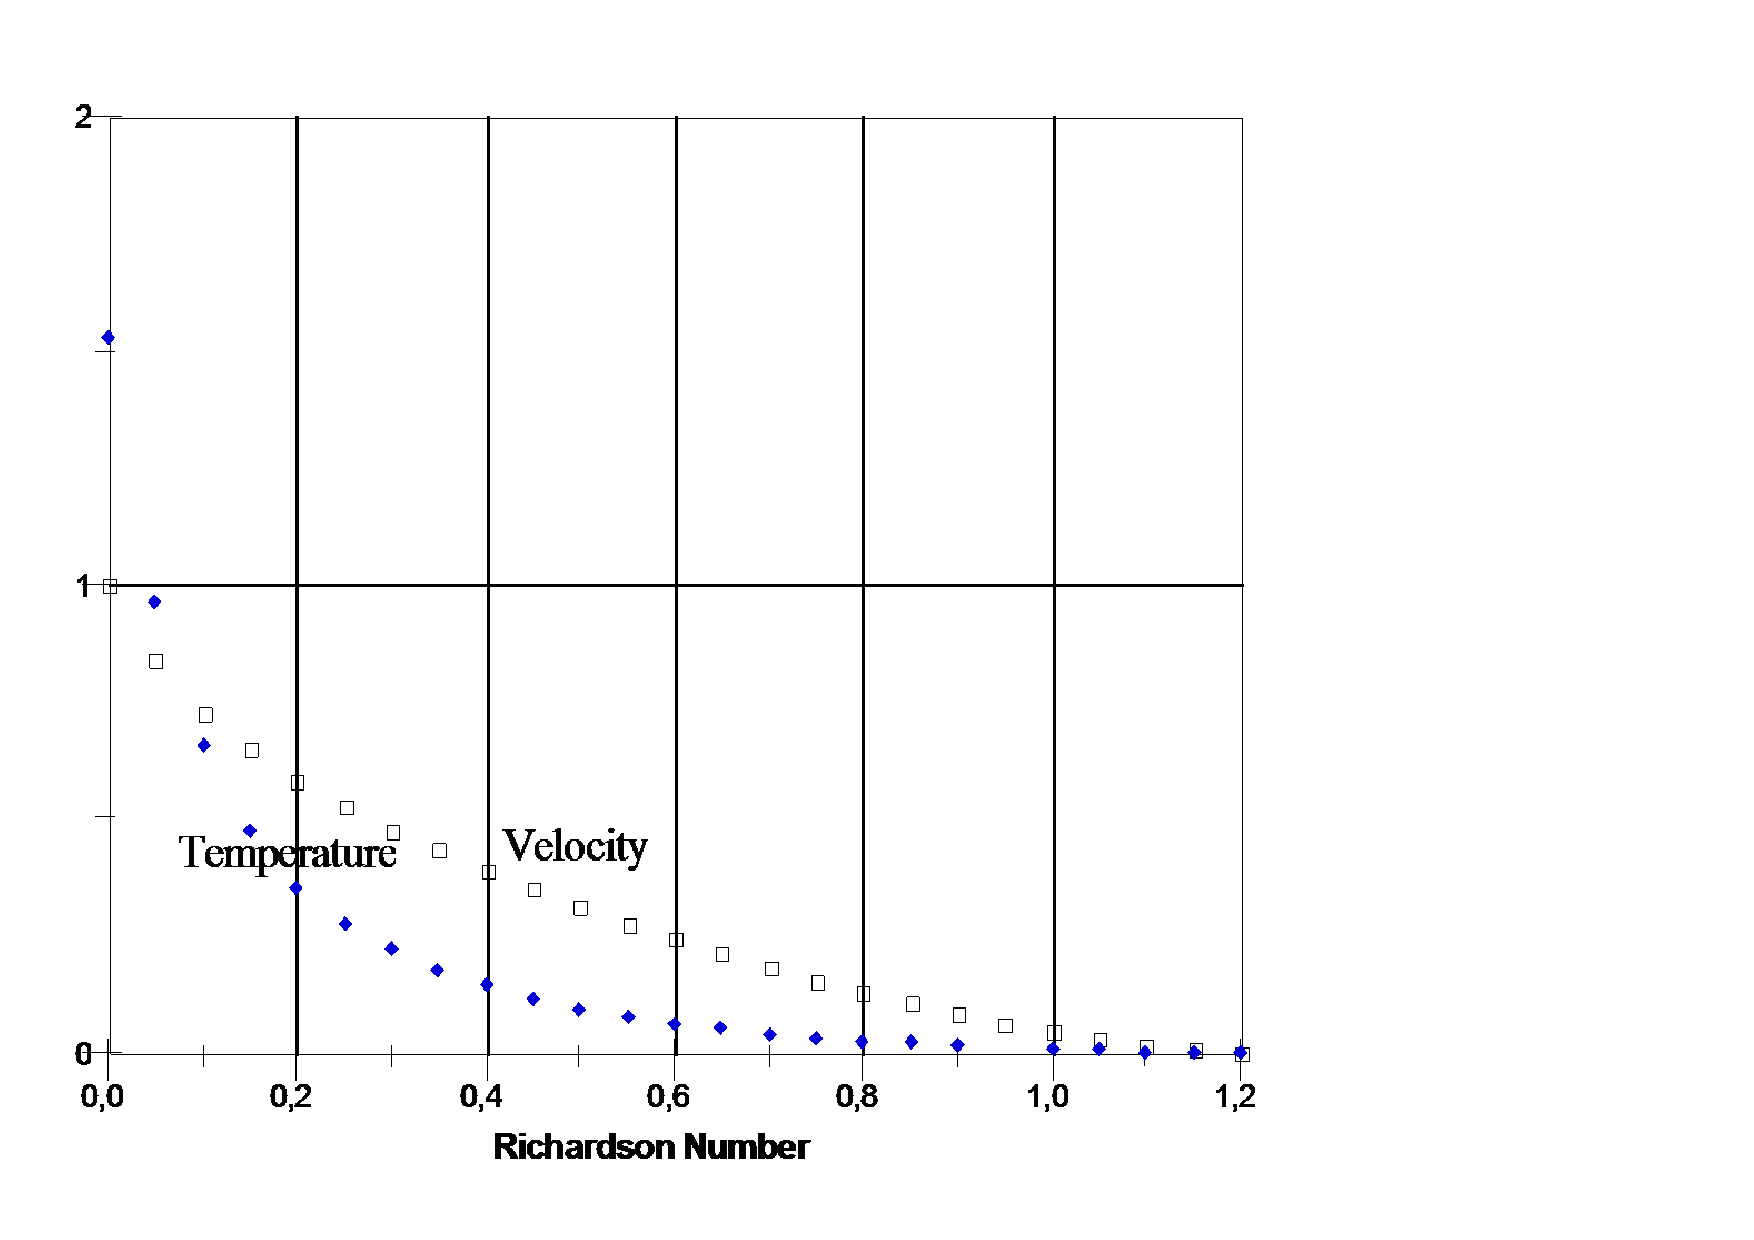
\includegraphics[scale = 0.5, trim=0 0 200 50, clip]{graphics/richardson.pdf}
  \caption{Damping functions on the velocity and scalar}
  \label{figure6}%
\end{figure}

The mixing length $L_{m}$ can be modelled in different ways:

\textbf{Classical} \textbf{Prandtl} \textbf{model} (see \cite{rodi84}):

$L_{m}=\kappa z$\ if $z\leq0.2h$ (here, $z$ is the distance to the bed and
$h$ the water depth).

$L_{m}=0.2\kappa h$\ if $z\geq0.2h$.

\textbf{Nezu and Nakagawa model} (see \cite{nezu93}):%

\[
L_{m}=\kappa z\sqrt{1-\dfrac{z}{h}}%
\]


In this case the mixing length vanishes at the free surface. This model can
give a logarithmic velocity profile from bed to free surface.

\textbf{Quetin} \textbf{model} (1977, see \cite{quetin77}):%
\index{Quetin model}%
%

\[
L_{m}=\dfrac{1}{\dfrac{1}{\kappa z}+\dfrac{1}{0.65d}}%
\]
where $d$ is the distance to the free surface.

\textbf{Tsanis model} (see \cite{tsanis89}):%
\index{Tsanis model}%


$L_{m}=\kappa z$\ if $z\leq0.2h$ (here, $z$ is the distance to the bed and
$h$ the water depth).

$L_{m}=0.2\kappa h$\ if $z\geq0.2h$ and $z\leq0.8h$.

$L_{m}=\kappa d$\ if $z\geq0.8h$ ($d$ is the distance to the free surface).

In the production of turbulence expression, the horizontal gradients of $u$
and $v$ as well as the gradients of $w$ are assumed negligible compared to the
vertical gradients. The term:
\[
\sqrt{\left(  \dfrac{\partial u}{\partial z}\right)  ^{2}+\left(
    \dfrac{\partial v}{\partial z}\right)  ^{2}}%
\]
is thus only an approximation of $\sqrt{2S_{ij}S_{ij}}$. For a calculation in
the vicinity of a structure (quay, spikes, etc.), the gradients overlooked
here can become important. However, their presence in the vertical viscosity
expression would not be of much help to perform an efficient calculation
around a structure. A mixing length model for horizontal viscosity would also
become necessary. Hence a precise computation of flow around structures is not
possible with this turbulence modelling.%



\subsubsection{\label{smagorinski}Smagorinski model%
  \index{Smagorinski model}%
}

The Smagorinski model (see \cite{smagorinski63}) has a meaning only in
numerical modelling and is based on the mixing length model. It belongs to the
category of sub-grid turbulence models. The principle is as follows:
turbulence is the solution of the Navier--Stokes equations. It would naturally
appear in the numerical solutions if the size of finite elements allowed the
reproduction of all mechanisms including the viscous dissipation of very small
vortices. Only in the formation of smaller vortices, where turbulence is
inhibited by the mesh, does modelling take place in a numerical simulation.
Smagorinski's idea is to add to the molecular viscosity a turbulent viscosity
deduced from a mixing length model. This mixing length corresponds to the size
of the vortices smaller than that of the mesh size. We simply arrive at the
following formulation:%

\begin{equation}
  \nu_T=C_{s}^{2}\Delta^{2}\sqrt{2S_{ij}S_{ij}}%
\end{equation}
where $C_{s}$ is a dimensionless coefficient to be calibrated and $\Delta$ the
mesh size derived in 2D or 3D from the surface or from the volume of the
elements. The values of $C_{s}$ range from 0.1 (flow in a canal) to 0.2
(isotropic turbulence). This model is best understood in 3D. In 2D it does not
take dispersion into account.


\subsection{\label{k-epsilon 3D}Two-equations $k$--$\epsilon$ model%
  \index{k--$\epsilon$ model|textbf}%
}

This model is based on the calculation of physical quantities representing
turbulence in the flow.
%$k$ and $\epsilon$ respectively designate turbulent
%kinetic energy%
%\index{turbulent kinetic energy}
%and its dissipation%
%\index{dissipation}%
%:%
%
%\begin{equation}
%  k=\dfrac{1}{2}\overline{u_{i}^{^{\prime}}u_{i}^{^{\prime}}}%
%\end{equation}
%%
%
%\begin{equation}
%  \epsilon=\nu\overline{\dfrac{\partial u_{i}^{^{\prime}}}{\partial x_{j}%
%    }\dfrac{\partial u_{i}^{^{\prime}}}{\partial x_{j}}}%
%\end{equation}
%where $u_{i}^{^{\prime}}$ is the turbulent fluctuation%
%\index{turbulent fluctuation}
%of velocity and where the bar represents averaging.

\subsubsection{$k$ and $\epsilon$ equations:}\label{sec:kepsequations}

The transport equation on $k$ is obtained by taking the trace of the transport equation on the Reynolds stresses, and reads:
\begin{equation}\label{eq:kEquation}
  \dfrac{\partial k}{\partial t} +\overline{\vec{u}}\cdot \Grad k= \mathbb P + \nabla \cdot \vec{Q}^k - \epsilon + \mathbb{G}
\end{equation}
where $\mathbb P$ is a production term whose definition is ~\mbox{$\mathbb P=-\vec{R}\!:\!\vec{S}$}.
By using the Boussinesq model~\eqref{eq:Boussinesq}, it can be written as%
\footnote{Strictly speaking, the term $-2/3 k \nabla \cdot \vec u$ should be taken into account for flows that are not truly incompressible.}:
\begin{equation}\label{eq:production}
  \mathbb P = \nu_T S^2
\end{equation}
with $S$ the scalar mean rate-of-strain defined as:
\begin{equation}\label{eq:scalarS}
  S = \sqrt{2\vec{S}:\vec{S}}
\end{equation}
$\mathbb{G}$ is a source term due to the forces of gravity in the case of temperature gradients.
It comes from the derivation of the Reynolds stress equation under the form: $\mathbb G = -\beta\vec{g}\cdot \overline{\vec{u}'T'}$, and thus also appears in the $k$ equation. This term is modelled through a turbulent thermal diffusivity model,
which yields:
\begin{equation}
\mathbb{G}=-\beta\dfrac{\nu_T}{Pr_T}g\dfrac{\partial \overline{T}}{\partial z}%
\end{equation}
with $\beta=-1/\rho(\partial\rho/\partial \overline{T})$, $Pr_T$ being the turbulent
Prandtl number.\index{Prandtl}%
In~\eqref{eq:kEquation}, $\vec{Q}^k$ is the flux of $k$, which represents a transport of
kinetic and potential energy by the eddies and the molecular viscosity.
The flux of $k$ can be modelled through a diffusion term:
\begin{equation}
  \nabla \cdot \vec{Q}^k = \dfrac{1}{\rho}\nabla \cdot \left(\mu_k \vec \nabla k\right)
\end{equation}
where $\mu_k$ is defined as $\mu_k = \mu+\mu_T/\sigma_k$, $\sigma_k$ being a model constant.
On the other hand, $\epsilon$ corresponds to a dissipation of turbulent kinetic energy (transformed into thermal energy) due to the viscosity, defined as:
\begin{equation}
  \epsilon = \nu \sum_i\sum_j\overline{\left(\dfrac{\partial u'_i}{\partial x_j}\right)^2}
\end{equation}
where $\partial u'_i/\partial x_j$  denotes the derivative of the $i$th component of $\vec u'$ with respect to the $j$th coordinate.
Although it is possible to write an exact transport equation on $\epsilon$, the latter includes complex terms that cannot be explicitly calculated.
This is why, in the $k-\epsilon$ model $\epsilon$ is computed through a simplified equation that reproduces the $k$ equation:
\begin{equation}\label{eq:epsilonEquation}
  \dfrac{\partial\epsilon}{\partial t}+\overline{\vec{u}}\cdot \Grad \epsilon =
C_{1\epsilon}\dfrac{\epsilon}{k}\left(\mathbb P+(1-C_{3\epsilon})\mathbb G\right)  -C_{2\epsilon}\dfrac{\epsilon^2}{k}
+ \dfrac{1}{\rho}\Div \left(\mu_\epsilon \vec \nabla \epsilon\right)
\end{equation}
where $\mu_\epsilon$ is defined as: $\mu_\epsilon = \mu+\mu_T/\sigma_\epsilon$, $\sigma_\epsilon$ being a constant.
$C_{1\epsilon}$ and $C_{2\epsilon}$ are also constants of the model (see the table~\ref{epsilon}).
The equation~\eqref{eq:epsilonEquation} has no theoretical background but relies on empirical considerations. The constant $C_{3\epsilon}$ was introduced in order to represent the fact that stable stratifications
weaken turbulence. It is thus taken as equal to one if $\mathbb G$ is negative, and zero otherwise.
The term $\epsilon/k$ is the frequency of the large eddies, it ensures the equation homogeneity.
The $\epsilon$ source terms are supposed proportional to the ones in the $k$ equation.\\

Note that the $k-\epsilon$ model is not accurate concerning non-inertial and streamline curvature effects, as well as severe deviation from local equilibrium.
Besides, it was shown that computing the production term through~\eqref{eq:production} leads to over-estimations of $k$ and thus of $\nu_T$.
In order to avoid this, Guimet \& Laurence~\cite{Guimet2002} proposed to restrict the production term to a linear behaviour for high values of the rate-of-strain,
obtained from the equilibrium between $\mathbb P$ and $\epsilon$ for fully developed homogeneous turbulence.
This yields a linear-quadratic model for the production%
\footnote{This essentially recovers the SST modification~\cite{Menter1994}, although it does not include a low-Reynolds treatment.}:
\begin{equation}\label{eq:P}
\mathbb P = \text{min}\left(\sqrt{C_\mu} k S, \nu_T S^2 \right)
\end{equation}
Another issue is that the size of the large eddies, given by $L_t \sim k^{3/2}/\epsilon$, may be predicted arbitrarily large, which is not physical since $L_t$ should
be bounded at least by $L$, the characteristic size of the flow.
To remedy this issue, Yap~\cite{Yap1987} proposed a modification of the $C_{2\epsilon}$ coefficient in order to increase the dissipation of turbulent kinetic energy:
\begin{equation}\label{eq:Cepsilon2_Yap}
  C_{2\epsilon,Y} = \text{max}\left(C_{2\epsilon} - \text{max}\left[ 0, 0.83\left(\dfrac{L_t}{L}-1\right)\left(\dfrac{L_t}{L}\right)^2 \right],0\right)
\end{equation}

\begin{CommentBlock}{Remark:}
By default the Yap treatment for $C_{2\epsilon}$ is not activated in \telemac{3d}.
This choice of option is hard-coded in the routine CSTKEP.f at the line 183.
\end{CommentBlock}

The Kolmogorov dimensional analysis~\cite{Kolmogorov1991} leads to a definition of the eddy viscosity as a function of $k$ and $\epsilon$,
which corresponds to the fact that the large turbulent eddies are the ones that most interact with the mean flow.
$\nu_T$ is thus written as proportional to the length scale of the large eddies, $L_t \sim k^{3/2}/\epsilon$, which yields:
\begin{equation}\label{eq:nut}
\nu_T = C_\mu \dfrac{k^2}{\epsilon}
\end{equation}
$C_\mu$ is the Prandtl-Kolmogorov constant.\\

The constants of the $k$--$\epsilon$ model have been determined by
comparison with simple situations. The constants $C_{\mu}$ and
$C_{1\epsilon}$ are obtained from data for turbulent flow near a rigid
wall. The free decay of grid turbulence helps us to find a value for
$C_{2\epsilon}$ on the basis of well-documented experimental data. The
constants $\sigma_{k}$ and $\sigma_{\epsilon}$ have been \textquotedblleft
optimised\textquotedblright, based on the performance of the model in both the
test cases just mentioned. Obtaining $C_{3\epsilon} $ is elaborated in
references \cite{launder74} and \cite{Viollet2002}. We retain that
$C_{3\epsilon}$ is equal to 1 for a stable situation, i.e. if $\mathbb G$ is
negative, and equal to 0 for unstable stratifications. $\sigma_{k}$ is
sometimes called \textquotedblleft Prandtl's turbulent number for the kinetic
energy of turbulence\textquotedblright.
All these constants are summarised in the table \ref{epsilon}.%

\textbf{Remarks:}
\begin{itemize}
\item {It is the equilibrium hypothesis between the creation of turbulence and
dissipation which leads to the mixing length model%
\index{mixing length model}%
. Actually, by assuming $\mathbb P=\epsilon$, and as $\nu_T\approx k^{2}/\epsilon$,
we immediately find $\nu_T\approx k^{2}/\mathbb P$. Also
$\nu_T\approx\sqrt{k}L_{t}$, where $L_{t}$ is the characteristic size of
vortices. We get:
\[\nu_T^{2}\approx\dfrac{k^{2}}{2S_{ij}S_{ij}}\]
and $\nu_T^{4}\approx k^{2}L_{t}^{4}$. By dividing the second equation by
the first one, member by member, we finally get:%

\[\nu_T\approx L_{t}^{2}\sqrt{2S_{ij}S_{ij}}\]
}
\item{In internal flow modelling, the term $-2/3 \, k\,\delta_{ij}$ is often
omitted because it plays the same role as pressure. If we want to have the
true pressure, it is not possible to integrate this term which should thus
appear in numerical resolution.
}
\end{itemize}

\begin{table}[tbp] \centering
  \caption{constants of the $k$--$\epsilon $ model  \label{epsilon}}$%
  \begin{tabular}
    [c]{|c|c|c|c|c|c|c|c|}\hline
    $\kappa$ & $C_\mu$ & $Pr_T$ & $C_{1\epsilon}$ & $C_{2\epsilon}$ &
    $C_{3\epsilon}$ & $\sigma_{k}$ & $\sigma_{\epsilon}$\\\hline
    0.41 & 0.09 & 1.0 & 1.44 & 1.92 & 0 if $\mathbb G>$ 0 and 1 if $\mathbb G\leq$ 0 & 1.0 &
    1.3\\\hline
  \end{tabular}
  \ $%
\end{table}%


\paragraph{\label{k-epsilon limites}Boundary conditions of the $k$%
  --$\epsilon$ model}

\paragraph{Rigid boundaries:}

to define rigid boundary conditions%
\index{boundary conditions!$k$--$\epsilon$ model},
it is considered that turbulence is in local equilibrium at the wall, such
that the production of turbulence (due to shear at the wall and at the bed)
is equal to dissipation and the velocity profile is locally logarithmic. This
idea was exploited by Mellor and Yamada to establish a zero-equation
turbulence model (see \cite{mellor74}).
With the equilibrium hypothesis, at a distance $\delta$ from the wall, the
$k$--$\epsilon$ model equations are:
\begin{equation}
  k=\dfrac{u_\ast^{2}}{\sqrt{C_{\mu}}}
\end{equation}

\begin{equation}
  \epsilon=\dfrac{u_\ast^{3}}{\kappa \delta}%
\end{equation}
The distance $\delta$ is chosen equal to 1/10th of the local mesh size,
measured along the normal direction to the wall. In the presence of
turbulence, the boundary condition for velocity is now written as:
\begin{equation}
\nu_T\dfrac{\partial u}{\partial n}=-u_\ast^{2}%
\end{equation}
$\nu$ being replaced by $\nu_T$.

\paragraph{Liquid boundaries:}

without additional information on the value of $k$ and $\epsilon$ at a
liquid boundary, a \textquotedblleft weak\textquotedblright\ condition is
applied, i.e. $\nu_T(\partial k/\partial n)=0$ and
$\nu_T(\partial\epsilon/\partial n)=0$. Such a condition can, however, give
rise to numerical problems at the entrance of a domain.

\paragraph{Free-surface:}
The treatment of boundary conditions on $k$ and $\epsilon$ at the free-surface
is tricky since it is not clear what to do in this case.
In \telemac{3d}, the following is done:
\begin{itemize}
\item the production term is considered quadratic at the free-surface:
\begin{equation}
\mathbb{P}=\nu_TS^2
\end{equation}
\item $\nu_T$ is calculated through the formula \eqref{eq:nut} but with a specific value of $k$.
The later is calculated based on the definition of the friction
velocity at the free-surface (obtained from the equation \eqref{eq:windstress}):
\begin{equation}
u_\ast|_{z=\eta}=\sqrt{a_{wind}\rho_{air}/\rho}~u_{wind}
\end{equation}
and considering that $k$ is defined by $k=u_\ast^2/\sqrt{C_\mu}$. The value
of $k$ at the free-surface is thus taken as:
\begin{equation}
k|_{z=\eta}=\left(\dfrac{a_{wind}\rho_{air}u_{wind}^2/\rho}{\sqrt{C_\mu}}\right)^2
\end{equation}
\end{itemize}

\begin{CommentBlock}{Remark:}
In the absence of wind the boundary condition on $k$ and $\epsilon$
at the free-surface is a zero-gradient.
However, the presence of the free-surface should reduce the length scale of the large eddies \cite{Hunt1984}.
A possibility to take this effect into account is to use the boundary condition on $\epsilon$
proposed in \cite{Celik1984}:
\begin{equation}
\epsilon_\eta=\dfrac{k_\eta^{3/2}}{\alpha h}
\end{equation}
where $\alpha \approx 0.18$ is an empirical constant, $k_\eta$ and $\epsilon_\eta$ are
the values of $k$ and $\epsilon$ at the free-surface and $h$ is the water depth.
\end{CommentBlock}

\subsection{Other models}

Though sufficiently difficult to implement numerically, the $k$--$\epsilon$
model has obvious limitations, particularly for eddies behind obstacles and in
the presence of a high rate of deformation (tensor $S_{ij}$) near a stagnation
point, for example. The Reynolds Stress Model (RSM) is a higher order model. The six
Reynolds stress%
\index{Reynolds!stress}
equations are then directly solved, and the $\epsilon$ equation, together
with the equations of scalar turbulent flux of temperature and salinity. Only
this type of model is capable of really taking into account turbulence
anisotropy by dropping the Boussinesq model. However, the triple
correlations of the equations are difficult to model and the boundary
conditions difficult to justify. This model has not been implemented in \telemac{3d} yet.
% To our knowledge, this is the reason why
% there is still no industry-oriented application of this model in free surface hydrodynamics.

\subsection{\label{contraintes turbulentes}Turbulent stress on the walls}

The presence of walls in turbulent flows makes the
latter anisotropic and increases the production of turbulence due to shearing effects.
Modelling near-wall turbulence is crucial in order to correctly reproduce the flows,
since the no-slip condition leads to large values of the velocity gradient at the walls,
which generates turbulence.
Let us denote by $y$ the distance to a wall and $y^+$ the dimensionless distance to a wall, defined as:
\begin{equation}\label{eq:yPlus}
  y^+=\dfrac{y u_*}{\nu}
\end{equation}
with $u_*$ a friction velocity, defined by:
\begin{equation}
  -\rho u_*^2\dfrac{\vec{u}_\tau}{u_\tau} = \vec{\tau} = \mu \left.\dfrac{\partial \vec{u}_\tau}{\partial y}\right|_{y=0}
\end{equation}
where $\vec{u}_\tau$ is the tangential velocity to the wall, $u_\tau$ its norm and $\vec{\tau}$ is the shear-stress,
with units \mbox{kg m$^{-1}$s$^{-2}$}.
The observation of the turbulent flow between two horizontal parallel plane walls (this configuration is called the plane Poiseuille channel)
led to a sub-division of the near-wall region into three areas~\cite{Viollet2002}:
\begin{itemize}
\item the viscous sub-layer: $0<y^+<8$
\item the buffer layer: $8<y^+<30$
\item the inertial sub-layer: $30<y^+<0.2e^+$
\end{itemize}
where $e^+$ is the dimensionless half-height of the channel, defined by $e^+=e u_{*}/\nu$ with $e$ the half-height.
The turbulence is negligible in the viscous sub-layer while the viscous effects are small in the inertial sub-layer.
In the latter, the velocity profile distribution along the normal to the wall follows a logarithmic law, so that this zone is also called the logarithmic zone.
If the characteristic roughness size of the wall is greater
than the thickness of the viscous sub-layer, this viscous sub-layer cannot
develop and the flow is known to be hydraulically rough. If there is a viscous
sub-layer the flow is known to be hydraulically smooth.
%To describe the velocity profile
%in the different layers, we consider a 1D flow for the sake of simplicity.
In the inertial layer, the velocity profile takes the following form:\\

\textbf{For hydraulically smooth flow:}\index{smooth flow}
\begin{equation}
  \dfrac{u_\tau}{u_*}=\dfrac{1}{\kappa}\ln\left(y^+\right)+5.2 \label{logarsmooth}
\end{equation}
For hydraulically smooth flow the linear and logarithmic laws are unified by
the Reichard law:
\begin{equation}
  \dfrac{u_\tau}{u_*}=\dfrac{1}{\kappa}\ln(1+\kappa y^{+})+7.8(1-e^{-\dfrac{y^{+}%
    }{11}})-\dfrac{y^{+}}{11}e^{-0.33y^{+}} \label{REICHARD}%
\end{equation}

\textbf{For hydraulically rough flow:}\index{rough flow}
\begin{equation}\label{eq:logarrough}
  \dfrac{u_\tau}{u_*}=\dfrac{1}{\kappa}\ln\left(  \dfrac{33 y}{k_{s}}\right)
  =\dfrac{1}{\kappa}\ln\left(  \dfrac{y}{k_{s}}\right)  +8.5
\end{equation}
where $k_{s}$ is the roughness size.
An equivalent way of writing the velocity profile for the hydraulically rough
flow is:%
\begin{equation}
  \dfrac{u_\tau}{u_*}=\dfrac{1}{\kappa}\ln\left(  \dfrac{y}{y_{o}}\right)
  \label{logarrough}%
\end{equation}
where$\;y_{o}\approx k_{s}/33$.
The reference \cite{Viollet2002} contains theoretical justifications of these formulae.\\

Directly simulating near-wall turbulence requires very fine
meshes and modified turbulence models (so-called low-Reynolds turbulence models).
Then, the computational points closest to the wall must be located in the viscous sub-layer.
This is computationally expensive, especially for flows with high-Reynolds numbers.
This led to the development of wall functions, based on semi-empirical formulae,
which are used to reproduce near-wall effects with coarser discretisations.
This corresponds to high-Reynolds-number turbulence models and requires
the computational points closest to the wall to be located in the inertial layer.
% Since RANS models were designed in order to coarsen the space-time discretisation, a wall boundary model is required in
% order to reproduce the effects of near-wall turbulence.
In Eulerian models, this can be done by designing the mesh so that
the first calculation point is in the logarithmic zone.
Another possibility is to solve the discretised equations
on a~'classical'~mesh, where the nodes located on the wall
are treated in the same way as if they were shifted in the
normal direction so as to be in the logarithmic zone, as for instance in~\cite{Kuzmin2007}.
%This makes it possible to resolve the region with more than one or two points.
This is done in \telemac{3d}: the velocity at the wall is taken in the boundary layer at a distance $y$.
$y$ is arbitrarily chosen or made to depend on the local mesh size
(\textit{e.g.} the edge point is at a distance from
the real wall equal to 1/10th of the size of the mesh).
Then, it is possible to specify the laws to be adopted in numerical
simulations to compute $u_*$ at the walls.
%In \telemac{3d}, only the case of hydraulically rough flows
%is considered (since in environmental flows, smooth regimes are
%hardly ever encountered).

\subsubsection{Hydraulically smooth flow%
  \index{smooth flow}%
}
By knowing $u_\tau$ and
$y$, the Reichard law (Equation \ref{REICHARD})\ gives $u_*$ from the
formula:
\index{Reichard law}
\begin{equation}
  \dfrac{u_*}{u_\tau}=\dfrac{1}{\dfrac{1}{\kappa}\ln(1+\kappa y^{+}%
    )+7.8(1-e^{-\dfrac{y^{+}}{11}})-\dfrac{y^{+}}{11}e^{-0.33y^{+}}}%
\end{equation}
This law is implicit as $y^{+}$\ depends on $u_*$, and $u_*$ is
found by successive iterations (10 iterations are done).
We then write:
\begin{equation}
  \nu\dfrac{\partial u_\tau}{\partial n}=-u_*{}^{2}%
\end{equation}

\subsubsection{Hydraulically rough flow}
Dimensional analysis
shows that $\vec{\tau}$ has the form:
\begin{equation}
\vec{\tau}=-\dfrac{1}{2}\rho C_{f}\vec{u}_\tau\vec{u}_\tau
\end{equation}
where $C_{f}$ is a dimensionless friction
coefficient. This general formula for shear forces supposes that
$\vec{u}_\tau$ is sufficiently far from the wall. It can also be written
as:
\begin{equation}
  \mu\dfrac{\partial\vec{u}_\tau}{\partial \vec{n}}=-\dfrac{1}{2}\rho C_{f}\vec{u}_\tau\vec{u}_\tau%
\end{equation}

The specification of the stress $\mu\partial\vec{u}_\tau / \partial \vec{n}$ will naturally appear in
the variational formulation of the diffusion terms in finite elements.
The bed shear stress condition will thus be ensured:
\begin{itemize}
\item Either by a turbulence model which will provide a formula for the stress
  $\mu (\partial\vec{u}_\tau / \partial \vec{n}$, based on the expression of
  the roughness at the bed and flow in the vicinity of the bed. Most
  often, the turbulence model gives the shear velocity $u_{\ast}$, or the
  friction coefficient $C_{f}$.

\item Or by knowledge of a friction coefficient $C_{f}$ and its associated
  velocity $\vec{u}_\tau$, which, due to the laws of bed shear stress
  in two dimensions, will be the average velocity on the vertical (the friction
  coefficients on the bed will thus be the same in two and three dimensions).
  This is the case of the Ch\'{e}zy, Strickler and Manning formulae:

  \textbf{Ch\'{e}zy formula:}%
  \index{Ch\'{e}zy!formula|textbf}
  ($C$ is the Ch\'{e}zy coefficient):%
  \begin{equation}
    C_{f}=\dfrac{2g}{C^{2}}%
  \end{equation}

  \textbf{Strickler formula:}%
  \index{Strickler!formula|textbf}
  ($S$ is the Strickler coefficient):%
  \begin{equation}
    C_{f}=\dfrac{2g}{h^{1/3}S^{2}}%
  \end{equation}

  \textbf{Manning formula:}%
  \index{Manning!formula}
  ($m$ is the Manning coefficient, equal to the inverse of the Strickler coefficient):%
  \begin{equation}
    C_{f}=\dfrac{2g\,m^{2}}{h^{1/3}}%
  \end{equation}
\end{itemize}
%In Section
%\ref{sec:solidBoundaries}\
%We have examined the Ch\'{e}zy, Strickler and Manning formulae.
%and Nikuradse formulae. For Nikuradse formula%
%\index{Nikuradse formula}%
%, we can now understand how it stems from the Ch\'{e}zy law and an integration
%vertically of the logarithmic profile given in Equation \eqref{eq:logarrough}.
When the roughness size $k_{s}$ is known, the following laws can also be used:\\

\textbf{Nikuradse formula:}%
\index{Nikuradse!formula}
This law stems from a depth-averaged value of the logarithmic turbulent velocity profile \eqref{eq:logarrough}.
The corresponding Chézy coefficient is obtained by the formula:%
\begin{equation}
  C=7.83\text{ln}\left(12\dfrac{h}{k_s}\right)
\end{equation}

\textbf{Haaland formula:}
\begin{equation}
  C_{f}=\dfrac{1}{4\left[0.6\ln\left(\left(\dfrac{6.9\nu}{4h\sqrt
            {u^{2}+v^{2}}}\right)^{3}+\dfrac{k_{s}}{14.8h}\right)\right]^{2}}
\end{equation}
\textbf{Ramette formula:}
according to Ramette \cite{ramette81}, the roughness size $k_{s}$ can also be
connected to the Ch\'{e}zy coefficient%
\index{Ch\'{e}zy!coefficient}
$C$ by the expression:
\begin{equation}
  C = \dfrac{26.4}{k_{s}^{1/6}}\left(\dfrac{k_{s}}{h}\right)^{1/24}h^{1/6}
\end{equation}
This last empirical formula is not dimensionless and requires a strict respect
of IS units.\\

\begin{CommentBlock}{Remark:}
In \telemac{3d}, there are options relying on the prescription of a friction coefficient,
with association to the depth-averaged velocity, because it seemed important to be able to
build a 3D model based on a 2D model without changing the calibration -- the Haaland, Chézy,
Strickler and Manning options. The Nikuradse
option, on the other hand, makes it possible to prescribe a friction based on a logarithmic
velocity profile for a given bed roughness, without any averaging of the velocity along the vertical.
It thus seems more appropriate than the depth-averaged models for the simulation of non quasi-horizontal flows.
\end{CommentBlock}
\newpage
\begin{CommentBlock}{Possible improvement for active scalars modelling:}
%\subsubsection{Turbulent boundary conditions on the temperature}
At the moment, in \telemac{3d} there is no treatment for the temperature boundary condition
when a Dirichlet condition is prescribed.
However, the temperature gradients close to the walls may be large in
turbulent mode, which generates turbulence as in the case of the velocity gradients.
If one were to consider applications where the scalar come close to a solid boundary,
it would be necessary to impose a wall function on the temperature with the $k-\epsilon$ model.
This is probably marginal but nevetheles the formulation is reported here.
Considering a 1-D fully developed flow field and thermal field in a channel,
the integration of the temperature equation along the normal to the wall,
from the wall to the centre of the channel reads:
\begin{equation}
  -Q_w = K_T \dfrac{d\overline T}{dy}
\end{equation}
where $y$ is the normal distance to the wall and $Q_w$ the heat flux applied at the wall.
Integrating once more yields:
\begin{equation}\label{eq:temperatureIntegral}
  \int_{T_w}^{\overline T} d\overline T = - Q_w \int_0^y\dfrac{dy}{K_T}
\end{equation}
where $T_w$ is the wall temperature. Defining the dimensionless variable
$T^+ = (T_w-\overline T)u_*/Q_w$, the equation~\eqref{eq:temperatureIntegral} can be written as:
\begin{equation}
  T^+ = \int_0^{y^+}\dfrac{\nu dy^+}{K_T}
\end{equation}
where $y^+$ is defined by~\eqref{eq:yPlus}. The integration of this equation can be done assuming a decomposition of the near-wall region into a laminar layer where $T^+$ varies linearly with $y^+$ and a turbulent layer where it follows a logarithmic law, as in~\cite{Bredberg2000}. It is also possible to use a three-layers model (see~\cite{Code_Saturne}) through:
\begin{equation}\label{eq:Tplus}
  \left\{\begin{array}{ll}
      T^+=Pr\hspace{0.05cm}y^+ & \text{if}~ y^+<y_1^+ \smallskip \\
      T^+=a_2-\dfrac{Pr_T}{2 a_1 \left(y^+\right)^2} &  \text{if}~ y_1^+ \le y^+<y_2^+ \smallskip \\
      T^+=\dfrac{Pr_T}{\kappa}\text{ln}~y^++a_3 &  \text{if}~ y^+>y_2^+ \smallskip \\
    \end{array}\right.
\end{equation}
where the following constants were defined:
\begin{equation}\label{eq:Tplus_constants}
  \left\{\begin{array}{l}
      y_1^+ = \left(\dfrac{a_{4}}{Pr}\right)^{1/3}~,~~~ y_2^+ = \sqrt{\dfrac{a_{4}\kappa}{Pr_T}}~,~~~a_1 = \dfrac{Pr_T}{a_{4}}, \smallskip \\
      a_2 = 15 Pr^{2/3}~,~~~a_3 = 15 Pr^{2/3} - \dfrac{Pr_T}{2\kappa}\left(1+\text{ln}~\dfrac{a_{4}\kappa}{Pr_T}\right)~,~~~ a_{4}=1000
    \end{array}\right.
\end{equation}
Recall that $\kappa$ is defined in the table~\ref{epsilon} and $Pr_T$ is the turbulent Prandtl number. Finally, $Pr=\dfrac{\nu}{K}$ is the molecular Prandtl number.
\end{CommentBlock}
%At the free-surface a homogeneous Neumann condition is imposed (no heat-flux).
%On the other hand, at inflow boundaries a Dirichlet condition is set on the temperature, whereas at outflow boundaries
%a homogeneous Neumann condition is prescribed (like for $k$ and $\epsilon$).
%%%%%%%%%%%%%%%%%%%%%%%%%%%%%%%%%%%%%%%%%%%%%%

\section{Modelling culverts in the flow}

\subsection{An example of application: a flood control area in the Scheldt estuary}

Flood Control Areas (FCA) together with a Controlled Reduced Tide (CRT) system
are implemented in the Scheldt estuary to reduce the risk of flooding.
The former is defined by an area specifically located in the regions where
the bottom elevation is lower than the mean tide elevation.
This area is surrounded by an outer higher dyke and in the interface with the river,
it has a lower dyke that allows the flow to overtop the structure during storm surges.
The CRT is based on the construction of inlet and outlet sluices that control the
flow between the river and the floodplain depending on the water levels on both
sides (see the figure \ref{fig:culvert_fig1}) \cite{Teles2015}.

\begin{figure}[H]
\begin{center}
  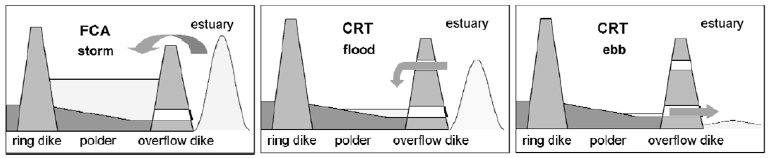
\includegraphics[width=0.95\textwidth]{graphics/culvert_fig1.png}
\end{center}
\caption{Water movements between the FCA and river without
CRT (on the left) and with CRT (on the middle and right pannels).
(Source: De Mulder et al. (2013)).}
\label{fig:culvert_fig1}
\end{figure}

The incorporation of these structures in numerical models is essential
to better predict and describe the flow hydrodynamics going to and
coming from these areas. The inlet and outlet sluices act like a weir
when they are not fully submerged and when water levels rise above the
inlet ceiling pressurised flow formulae are used.
The calibration of the head loss coefficients for the inlet and outlet sluices
was done comparing model results with measured water levels and discharges of
one specific CFA/CRT, called Lippenbroek.
Later these values were validated using the measurements from the CFA/CRT Bergenmeersen.
The coefficients found in this calibration/validation exercise are used for all the
other inlet and outlet sluices for the other FCA, FCA/CRT areas in the 3D model.

\subsection{Flow through a culvert: theoretical background}

A number of studies regarding the description of flows through the culverts
refer to Bodhaine's work \cite{Bodhaine1968}.
Bodhaine categorized the flow through a culvert into six types, and for each type
the discharge is calculated in a different way.
The equations are deduced from the continuity and energy equations between the approach
section (see the figure \ref{fig:culvert_fig2}) and the exit (downstream) section of the culvert.
The type of flow depends on whether the culvert flows full and whether the flow is controlled
by the entrance or exit part of the culvert. The figure \ref{fig:culvert_fig2}
shows a sketch for culvert flow definition.

\begin{figure}[H]
\begin{center}
  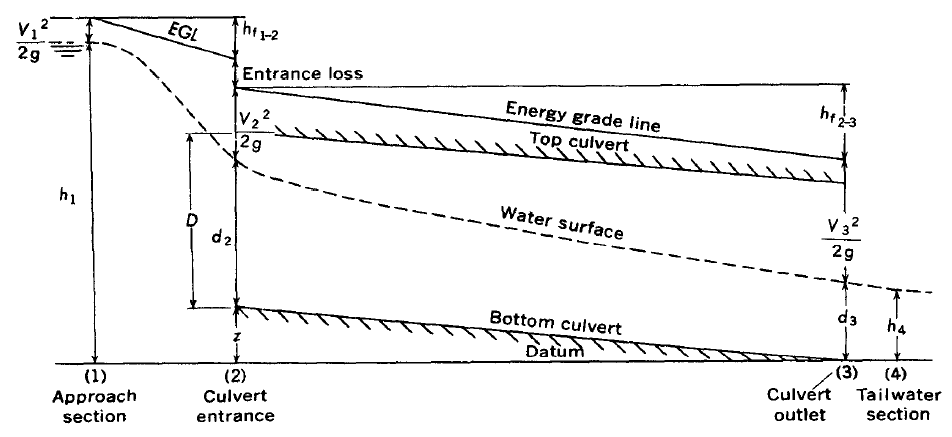
\includegraphics[width=0.95\textwidth]{graphics/culvert_fig2.png}
\end{center}
\caption{Sketch of general flow through a culvert \cite{Bodhaine1968}.}
\label{fig:culvert_fig2}
\end{figure}

$Z$ gives the elevation of the culvert entrance relative to the datum through the culvert exit.
The gravitational constant is given by $g$ and $h_{f12}$ is the head loss due to friction from
the approach section to the culvert entrance;
$h_{f23}$ is the head loss due to friction inside the culvert, $d_2$ and $d_3$ are the water
depths at the culvert entrance and exit, respectively;
$V_1$, $V_2$ and $V_3$ are the velocities at the approach section,
culvert entrance and culvert exit, respectively;
$D$ is the culvert height;
and $h_1$ and $h_4$ are the water depths upstream and downstream of the culvert structure.
The six types of flow classified by Bodhaine \cite{Bodhaine1968} depend on the water depths
upstream and downstream of the culvert.
The figure \ref{fig:culvert_fig3} gives a schematization of the different flow types
made according to the equation for each type of flow.
The different equations are presented below.

\begin{figure}[H]
\begin{center}
  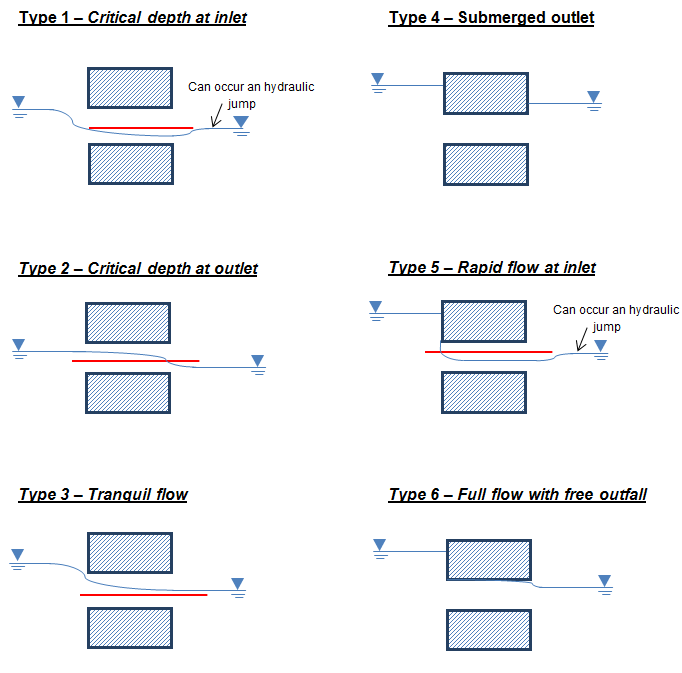
\includegraphics[width=0.7\textwidth]{graphics/culvert_fig3.png}
\end{center}
\caption{Sketch of the 6 different types of flow that occur
through culverts according to Bodhaine \cite{Bodhaine1968}.
The red line represents the critical water depth.}
\label{fig:culvert_fig3}
\end{figure}

\underline{\textbf{Type 1 -- Critical depth at inlet- supercritical flow at the entrance}}\\

In flow type 1 the flow is supercritical inside the culvert and the critical depth occurs
at the entrance of the culvert. The culvert slope ($S_0$) has to be greater than the
critical slope ($S_c$) and the culvert flows partially full.
For the Froude number $Fr=1$ (which is the case of flow type 1),
the discharge coefficient is typically $C_D=0.95$.
The discharge is then calculated according to the following formula:

\begin{equation}
Q = C_D A_c \sqrt{2g\left(h_1-z-h_c-h_{f12}+\alpha \dfrac{\overline{V_1}^2}{2g}\right)}
\end{equation}

with:\\
$C_D$ the discharge coefficient;\\
$A_c$ the flow area at critical water depth; \\
$g$ the gravitational constant; \\
$h_1$ the upstream water depth; \\
$z$ elevation of the culvert entrance; \\
$h_c$ the critical water depth; \\
$h_{f12}$ the head loss due to friction from the approach section to the culvert entrance; \\
$\alpha$ the kinetic energy correction coefficient for the approach section; \\
$V_1$ the average flow velocity at the approach section of the culvert.\\

\underline{\textbf{Type 2 -- Critical depth at outlet – supercritical flow at the exit}}\\

In flow type 2 the flow is tranquil inside the culvert. The critical depth is located at
the culvert outlet. The culvert flows partially full. Here the culvert slope has to be
smaller than the critical slope. The discharge coefficient is similar to flow type 1.
The discharge is then calculated according to the following formula:
\begin{equation}
Q=C_D A_c \sqrt{2g\left(h_1-h_c-h_{f12}-h_{f23}+\alpha \dfrac{\overline{V_1}^2}{2g}\right)}
\end{equation}
with:\\
$h_{f23}$ the head loss due to friction inside the culvert.\\

\underline{\textbf{Type 3 -- Tranquil flow -- subcritical flow}}\\

In flow type 3 the flow is subcritical inside the culvert. There is no critical depth.
The culvert flows partially full. Like flow types 1 and 2, the discharge coefficient
varies with respect to the Froude number, being typically between $C_D=0.82 -- 0.95$.
The discharge is calculated according to the following formula:
\begin{equation}
Q=C_D A_3 \sqrt{2g\left(h_1-d_3-h_{f12}-h_{f23}+\alpha \dfrac{\overline{V_1}^2}{2g}\right)}
\end{equation}
with:\\
$A_3$ the flow area at the culvert outlet;\\
$d_3$ the water depth at the culvert outlet.\\

\underline{\textbf{Type 4 -- Submerged inlet and outlet}}\\

In flow type 4 the culvert inlet and outlet are submerged. The culvert flows full.
The discharge coefficient varies with respect to the culvert geometry, ranging
typically between $C_D=0.75$ and $C_D=0.95$.
The discharge is calculated according to the following formula:
\begin{equation}
Q=C_D A_0 \sqrt{2g\dfrac{h_1-h_4}{1+29C_D^2 n^2 L/R^{4/3}}}
\end{equation}
with:\\
$A_0$ the flow area at the culvert entrance;\\
$h_4$ the downstream water depth;\\
$n$ the Manning coefficient;\\
$L$ the length of the culvert;\\
$R$ the hydraulic radius.\\

\underline{\textbf{Type 5 -- Rapid flow at inlet}}\\

In flow type 5, the flow is supercritical at the inlet to the culvert.
The culvert flows partially full. Type 5 flow does not usually occur.
When it does, the discharge coefficient is in general lower than the other types.
\begin{equation}
Q=C_D A_0 \sqrt{2g(h_1-z)}
\end{equation}

\underline{\textbf{Type 6 -- Full flow with free outfall}}\\

In flow type 6 the culvert flows full. The discharge coefficient is similar to the
one obtained for the flow type 4.
The discharge is calculated according to the following formula:
\begin{equation}
Q=C_D A_0 \sqrt{2g(h_1-d_3-h_{f23})}
\end{equation}
The indices of the different variables might seem a bit confusing,
but it was chosen to take the formulae from Bodhaine as they were
and not to make any changes to them.
Bodhaine differentiated between these six flow types based on conditions
given in the table \ref{tab:culvert_tab1}.

\begin{table}[H]
\caption{Conditions for each type of flow defined by Bodhaine \cite{Bodhaine1968}.}\label{tab:culvert_tab1}
\begin{center}\begin{tabular}{|c|c|c|c|}
\hline
~ & $\mathbf{\dfrac{h_1-z}{D}}$ & ~ & ~\\
\hline
\textbf{Type 1} & $<1.5$    &  $\frac{h_4}{h_c} < 1.0$ & $S_0 > S_c$\\
\hline
\textbf{Type 2} & $<1.5$    &  $\frac{h_4}{h_c} > 1.0$ & $S_0 < S_c$\\
\hline
\textbf{Type 3} & $<1.5$    & $\frac{h_4}{D} \le 1.0$ & ~\\
\hline
\textbf{Type 4} & $> 1.0$   & $\frac{h_4}{D} > 1.0$ & ~\\
\hline
\textbf{Type 5} & $\ge 1.5$ & $\frac{h_4}{D} \le 1.0$ & ~\\
\hline
\textbf{Type 6} & $\ge 1.5$ & $\frac{h_4}{D} > 1.0$  & ~\\
\hline
\end{tabular}\end{center}
\end{table}

All the different culvert geometric features will affect the presence of culvert flow type 5 or 6.
To differentiate the two types, Bodhaine \cite{Bodhaine1968} suggests to use the relations given in the figure \ref{fig:culvert_fig4}.
$r$ is the radius of entering rounded and $w$ is the measure of the length of a wingwall
or chamfer. First a curve corresponding to $r/D$, $w/D$ is chosen.
Then a point is set using the value for the culvert slope and for the ratio
between the culvert length and height.
If the point lies to the right of the chosen curve, the flow is type 6,
if it lies to the left of the curve, the flow is type 5.

\begin{figure}[H]
\begin{center}
  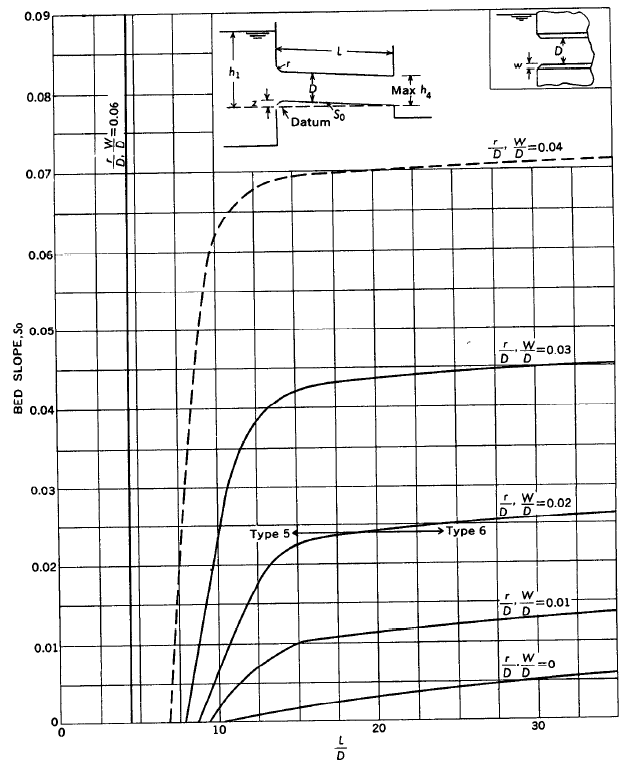
\includegraphics[width=0.6\textwidth]{graphics/culvert_fig4.png}
\end{center}
\caption{Criterion for classifying flow types 5 and 6 in concrete box or pipe culverts
with square, rounded, or bevelled entrances, either with or without wingwalls \cite{Bodhaine1968}.}
\label{fig:culvert_fig4}
\end{figure}

The head loss coefficients are subject of different studies made in laboratory experiments.
A number of authors have arrived to different values or empirical relationships for the
head loss coefficients. For instance, Bodhaine \cite{Bodhaine1968} suggests different values for
the discharge coefficient ($C_D$) for each type of flow and depending on a number of
geometric features from the culvert. The discharge coefficients can vary from 0.39 to 0.98.
Another example is Carlier \cite{Carlier1972} who proposes a non-dimensional coefficient $\mu$,
that for hydraulic structures made of only one culvert can be written as follows:
\begin{equation}
\mu = \dfrac{1}{\sqrt{C_1+C_2+C_3}}
\end{equation}
with:\\
$C_1$ the head loss coefficient at the entrance of the hydraulic structure;\\
$C_2$ the head loss coefficient in the hydraulic structure;\\
$C_3$ the head loss coefficient at the exit of the hydraulic structure.

If the general expression for the discharge $Q=\mu A \sqrt{2g\Delta H}$ proposed by
Carlier \cite{Carlier1972} is compared with the formulae given by Bodhaine \cite{Bodhaine1968},
it can be seen that the non-dimensional head loss coefficient ($\mu$),
incorporates both the effect of the discharge coefficient ($C_D$) and the continuous
and local head losses. $\Delta H$ is the head loss for each type of flow.

\subsection{Formulations for culvert simulation in TELEMAC}

TELEMAC-2D and 3D give the possibility of modelling hydraulic structures, such as bridges,
discharges under a dike or tubes in which free-surface or pressurized flows may
occur during the total simulation time.
This is done by a couple of points between which flow may occur with respect to
the water levels in the river and in the floodplain.
The subroutine BUSE is called to model this kind of structures.
Each kind of flow has its own type of discharge calculation.
The kind of formulation used to compute the flow rates can be chosen with the keyword OPTBUSE.

\subsubsection{Option 1 -- following Carlier's formulation}

With this first option, the different equations implemented to calculate the
discharges are dependent on the flow regime and follow Carlier \cite{Carlier1972}.
Then the velocities are deduced from the discharges and are taken into account as source
terms both in the continuity and momentum equations.
The critical water depth ($h_c$) is approximated to $h_c \approx 2/3 h_1$ \cite{Carlier1972}.
The figure \ref{fig:culvert_fig5} presents the different variables used to calculate the discharges.
$S_1$ and $S_2$ are the upstream and downstream water elevations, respectively, $z_1$ and $z_2$
the upstream and downstream culvert bottom elevations, $D$ the culvert height and $h_1=S_1-z_1$
and $h_2=S_2-z_2$ the upstream and downstream water depths, respectively.

\begin{figure}[H]
\begin{center}
  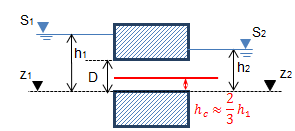
\includegraphics[width=0.5\textwidth]{graphics/culvert_fig5.png}
\end{center}
\caption{Representation of the different variables used to calculate
the discharges for each type of flow.}
\label{fig:culvert_fig5}
\end{figure}

The equations coded with this first option are described below.
Between brackets the corresponding flow type according to Bodhaine \cite{Bodhaine1968} is given.
\begin{itemize}
\item Free surface flow equations:
  \begin{itemize}
  \item Submerged weir (Bodhaine type 3)
    \begin{equation}
      Q=\mu (S_2-z_2) W \sqrt{2g(S_1-S_2 )} = (S_2-z_2) W \sqrt{\dfrac{2g(S_1-S_2)}{C_1+C_2+C_3}}
    \end{equation}
  \item Unsubmerged weir(Bodhaine type 2)
    \begin{equation}
      Q=0.385 W \sqrt{2g}(S_1-z_1)^{3/2}
    \end{equation}
  \end{itemize}
\item Pressurised flow equations:
  \begin{itemize}
  \item Submerged orifice law (Bodhaine type 4)
    \begin{equation}
      Q=\mu D W \sqrt{2g(S_1-S_2 )} = D W \sqrt{\dfrac{2g(S_1-S_2)}{C_1+C_2+C_3}}
    \end{equation}
  \item Unsubmerged orifice law
    \begin{equation}
    Q= \mu D W \sqrt{2g(S_1-S_2)} = D W \sqrt{\dfrac{2g(S_1-S_2)}{C_1+C_2}}
    \end{equation}
  \end{itemize}
\end{itemize}

The user has the possibility of assigning different values for $C_1$, $C_2$ and $C_3$.
The flow direction is imposed, \textit{e.g.}, the user can specify if the flow is going
in only one direction or in both directions and in which direction.
The keyword CLP specifies this behaviour.\\
CLP=0, flow is allowed in both directions;\\
CLP=1, flow is only allowed from section 1 to section 2\\
CLP=2, flow is only allowed from section 2 to section 1\\
CLP=3, no flow allowed.\\
A relaxation parameter ($\theta$) is introduced so that the discharge is calculated
in an explicit, implicit, or semi-implicit way.
If $\theta=1$ the calculation of the discharge is explicit while if $\theta=0$
the discharge calculation is implicit:
\begin{equation}
  Q^n=\theta Q^n + (1-\theta) Q^{n-1}
\end{equation}
Relaxation gives slower convergence speed to get the final solution
but smoothes some instabilities.
If the solution does not converge because of instabilities, the coefficient can be lowered.

\subsubsection{Option 2 -- following Bodhaine's formulation}

With this option the discharges are calculated based on the equations proposed in \cite{Bodhaine1968}
and similar to the ones incorporated in DELFT 3D model.
The flow type 1 conditions were not incorporated since they only
occur when the culvert slope is larger than the critical flow slope.
This only happens in very rare occasions if the culvert slope is very steep.
The equations used to compute the discharges are given below.\\

\underline{\textbf{Type 2 -- Critical depth at outlet}}\\
\begin{equation}
Q = \mu h_c W \sqrt{2g(S_1-(z_2+h_c))}
\end{equation}
with:
\begin{equation}
\mu = C_{D1}/\sqrt{1+\left[\dfrac{2gLn^2}{R^{4/3}} +C_v\right] C_{D1}^2 \dfrac{h_c}{h_s}^2}
\end{equation}
\begin{equation}
h_s=0.5h_c+0.5(S_1-z)
\end{equation}
\begin{equation}
R=\dfrac{h_s W}{2h_s+W}
\end{equation}

\underline{\textbf{Type 3 -- Tranquil flow}}\\
\begin{equation}
Q=\mu (S_2-z_2)W\sqrt{2g(S_1-S_2 )}
\end{equation}
with:
\begin{equation}
\mu = C_{D1}/\sqrt{ 1+\left[\dfrac{2gLn^2}{R^{4/3}} +C_v \right] C_{D1}^2 \left(\dfrac{S_2-z_2}{h_s}\right)^2}
\end{equation}
\begin{equation}
h_s=0.5(S_1-z)+0.5(S_2-z)
\end{equation}
\begin{equation}
  R=\dfrac{h_sW}{2h_s+W}
\end{equation}

\underline{\textbf{Type 4 -- Submerged outlet}}\\
\begin{equation}
Q =\mu D W \sqrt{2g(S_1-S_2)}
\end{equation}
with:
\begin{equation}
\mu = C_{D2}/\sqrt{1+\left[\dfrac{2gLn^2}{R^{4/3}} +C_v \right] C_{D2}^2}
\end{equation}
\begin{equation}
h_s=D
\end{equation}
\begin{equation}
R=\dfrac{h_s W}{2h_s+2W}
\end{equation}

\underline{\textbf{Type 5 -- Rapid flow at inlet}}\\
\begin{equation}
Q= \mu D W \sqrt{2gh_1}
\end{equation}
with:
\begin{equation}
\mu = C_{D3}
\end{equation}
\begin{equation}
h_s = D
\end{equation}
\begin{equation}
R = \dfrac{h_s W}{2h_s+2W}
\end{equation}

\underline{\textbf{Type 6 -- Full flow with free outfall}}\\
\begin{equation}
Q = \mu D W \sqrt{2g(S_1-(z_2+D))}
\end{equation}
with:
\begin{equation}
\mu = C_{D2}/\sqrt{1+\left[\dfrac{2gLn^2}{R^{4/3}} +C_v \right] C_{D2}^2}
\end{equation}
\begin{equation}
h_s=D
\end{equation}
\begin{equation}
R=\dfrac{h_s W}{2h_s+2W}
\end{equation}
The head loss coefficient expressions were obtained from experimental studies made at
Flanders Hydraulic Research.
The discharge coefficient, $C_D$, is dependent of each type of flow, being the same for
types 1, 2 and 3 ($C_{D1}$), then for types 4 and 6 ($C_{D2}$) and finally for type 5 ($C_{D3}$).
The conditions at which a certain type of flow occurs,
are presented in the table \ref{tab:culverts_tab2}.

\begin{table}[H]
\caption{Conditions for each type of flow used in TELEMAC with OPTBUSE = 2.}
\label{tab:culvert_tab2}
\begin{center}\begin{tabular}{|c|c|c|c|c|}
\hline
~ & $\mathbf{\dfrac{S_1-z_1}{D}}$ & $\mathbf{\dfrac{S_2-z_2}{D}}$ & $\mathbf{S_2-z_2}$ & $L/D$ \\
\hline
\textbf{Type 2} & $<1.5$    &  ~ & $< h_c$ & ~ \\
\hline
\textbf{Type 3} & $<1.5$    & $\le 1.0$ & $> h_c$ & ~\\
\hline
\textbf{Type 4} & $> 1.0$   & $> 1.0$ & ~ & ~\\
\hline
\textbf{Type 5} & $\ge 1.5$ & $\le 1.0$ & ~ & $< h_c$\\
\hline
\textbf{Type 6} & $\ge 1.5$ & $\le 1.0$  & ~ & $\ge h_c$\\
\hline
\end{tabular}\end{center}
\end{table}

The equations presented above are written to describe flow conditions through a
culvert system with a single pipe.
Nevertheless, additional features are sometimes incorporated in the hydraulic structures,
such as weirs in the vicinity of the culvert entrance or exit.
Such combined structures have to be taken into account.
Then the geometric features of the culvert presented in the figure \ref{fig:culvert_fig5}
are modified (see the figure \ref{fig:culvert_fig6}).
It was decided that an equivalent culvert bottom elevation should be used,
which replaces both the bottom elevations $z_1$ and $z_2$ in the formulae decribed above.
The equivalent bottom culvert elevation is then equal to the mean between $z_1$ and $z_2$.
The diameter used in the equations will be the one corresponding to the entrance of the culvert,
\textit{i.e.}, regarding the figure \ref{fig:culvert_fig6}, if the flow goes from left
to the right $D$ will be replaced by $D_1$ and on the opposite direction,
the value $D_2$ will be used.

\begin{figure}[H]
\begin{center}
  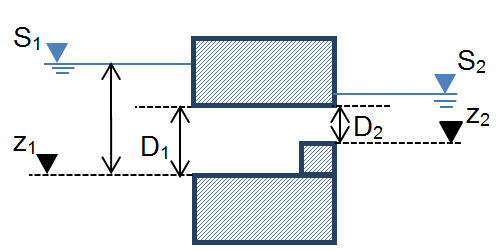
\includegraphics[width=0.5\textwidth]{graphics/culvert_fig6.png}
\end{center}
\caption{Representation of the different variables used to
calculate the discharges for each type of flow.}
\label{fig:culvert_fig6}
\end{figure}

The head loss coefficient ($\mu$ was adapted from the one calculated with the first option,
based on Carlier \cite{Carlier1972} and is used as main head loss coefficient).
Structures that caused additional head loss, like valves, grilles (trash screens) or pilars
were added in the calculation of this main coefficient.
In this way these additional features that can be present in culvert structures of
different geometric configurations are taken into account and contribute to
the flexibility of the implementation of many types of culvert structures.
The head loss due to singularities can be obtained by the general
relation \cite{Lencastre1961}, \cite{Carlier1972}:
\begin{equation}
\Delta H = C \dfrac{U^2}{2g} ~\text{or}~  U = \mu \sqrt{2g\Delta H}
\end{equation}
with:
\begin{equation}
\mu =\dfrac{1}{\sqrt{C}}
\end{equation}

The coefficient $C$ represents the sum of the different contributions for the
head loss due to singularities:
\begin{equation}
C=C_1+C_p+C_2+C_3+C_v+C_T
\end{equation}
The different contributions to this head loss coefficient $C$ will be discussed
separately and in detail here below.\\

\textbf{Coefficient} $\mathbf{C_1}$ \\
$C_1$ represents the head loss due to the contraction of the flow at the entrance
of the hydraulic structure.
Usually it is equal to 0.5 (figure \ref{fig:culvert_fig7}).
Usually, there is an abrupt contraction that will cause a head loss due to
the decelaration of the flow immediately after the culvert entrance.

\begin{figure}[H]
\begin{center}
  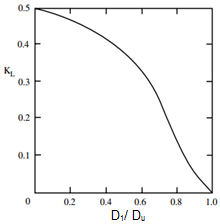
\includegraphics[width=0.5\textwidth]{graphics/culvert_fig7.png}
\end{center}
\caption{Local loss coefficient for a sudden contraction as
a function of diameter ratio between the diameter after the contraction ($D_1$)
and before the contraction $D_u$ \cite{Bruce2000}.}
\label{fig:culvert_fig7}
\end{figure}

Already in the past, Bodhaine \cite{Bodhaine1968} noticed that the discharge coefficient ($C_D$)
for type 5 flow had to be lowered comparetively with the other flow types.
It seems that the calculated discharge tends to be overestimated when the
default equation is applied. In order to take into account that effect,
a correction coefficient ($\alpha_1^5$) is applied to $C_1$ when type 5 flow occurs, such that:
\begin{equation}
\Delta H_{1.5}=\alpha_1^5 C_1  \dfrac{U^2}{2g}
\end{equation}
Comparing with the values proposed in \cite{Bodhaine1968}, $4 \le \alpha_1^5 \le 10$.\\

\textbf{Coefficient} $\mathbf{C_p}$\\
Sometimes at the entrance of culverts the flow is divided into two sections
caused by two entrance boxes instead of one but than the flow converges into
a single culvert pipe. In other words a kind of pilar is dividing the flow at the entrance.
This causes additional head loss and is taken into account.
Following Carlier \cite{Carlier1972} the head loss through parallel pillars is given by:
\begin{equation}
\Delta H_p = C_p \dfrac{U^2}{2g}
\end{equation}
where $C_p=\beta \left(Lp/b\right)^{4/3} \text{sin} \theta$  represents the head
loss coefficient due to the presence of pillars. $Lp$ is the thickness of the pillars, $b$
the free thickness between two consecutive pillars and $\beta$
a coefficient dependent on cross-shore section of the pillar.\\

\textbf{Coefficient} $\mathbf{C_2}$\\
$C_2$ represents the head loss coefficient due to the friction in the structure
and is expressed by (Lencastre, 1972):
\begin{equation}
\Delta H_2 = C_2  \dfrac{U^2}{2g} = \dfrac{2gLn^2}{R^{4/3}}\dfrac{U^2}{2g}
\end{equation}
where $L$ is the length of the structure, $n$ the Manning Strickler coefficient
of the structure and $R$ the wet cross-shore section in the structure calculated
in the code for each type of flow.
The table \ref{tab:culvert_tab3} presents the expressions for the calculation of $R$,
following what was done in the DELFT 3D model.
Here an assumption is made when calculating the hydraulic radius since the
code does not make any kind of backwater analysis to get the
precise water depths that occur in the culvert (like Mike 11 does).
\begin{table}[H]
\caption{Different parameters for each type of flow to calculate the hydraulic radius in \telemac{3d}.}
\label{tab:culvert_tab3}
\begin{center}\begin{tabular}{|c|c|c|}
\hline
\textbf{Type of flow} & $\mathbf{h_s}$ & $\mathbf{R}$ \\
\hline
\textbf{Type 2} & $0.5 h_c + 0.5(S_1-z)$    & $R = \dfrac{h_s W}{2 h_s+W}$ \\
\hline
\textbf{Type 3} & $0.5 (S_1 - z_1) + 0.5(S_2-z_2)$    & $R = \dfrac{h_s W}{2 h_s+W}$ \\
\hline
\textbf{Type 4} & $D$    & $R = \dfrac{h_s W}{2 h_s+2W}$ \\
\hline
\textbf{Type 5} & $D$    & $R = \dfrac{h_s W}{2 h_s+2W}$ \\
\hline
\textbf{Type 6} & $D$    & $R = \dfrac{h_s W}{2 h_s+2W}$ \\
\hline
\end{tabular}\end{center}
\end{table}

\textbf{Coefficient} $\mathbf{C_3}$\\
$C_3$ is the head loss coefficient due to expansion of the flow exiting the culvert.
It can be given by \cite{Lencastre1961}:
\begin{equation}
\Delta H_3 = \left(1-\dfrac{A_s}{A_{s2}}\right)^2 \dfrac{U^2}{2g} = C_3\dfrac{U^2}{2g}
\end{equation}
where $A_s$ and $A_{s2}$ are the sections in and at the downstream part of the structure.
Usually is equal to the unity for a sudden enlargement.\\

\textbf{Coefficient} $\mathbf{C_V}$\\
$C_V$ is the head loss coefficient due to the presence of a valve.
The head loss due to valves ($\Delta H_v$) can also be estimated:
\begin{equation}
\Delta H_v = C_V\dfrac{U^2}{2g}
\end{equation}
where $C_V$ depends on the type of valve and the degree of opening.
For a gate valve, some values were obtained experimentally,
and they depend on the opening of the valve \cite{Bruce2000}:
see the table \ref{tab:culvert_tab4}.
\begin{table}[H]
\caption{Values for the head loss coefficient depending on the opening of a gate valve.}
\label{tab:culvert_tab3}
\begin{center}\begin{tabular}{|c|c|}
\hline
~ & $C_V$ \\
\hline
\textbf{Wide open} & 0.2\\
\hline
\textbf{3/4 open} & 1.0 \\
\hline
\textbf{1/2 open} & 5.6 \\
\hline
\textbf{1/4 open} & 17 \\
\hline
\end{tabular}\end{center}
\end{table}

Again, a correction coefficient ($\alpha_v^5$) is applied to the head loss coefficient
due to a valve in order to take into account the increase of the head loss when type 5
flow occurs.
Through a number of laboratory experiences (IMDC Report 613\_9\_1), it can be seen that when
type 5 flow occurs, there is a greater influence of having a valve:
the associated head loss coefficient is in general much higher than for the other types of
flow (see the figure  \ref{fig:culvert_fig8}).
Please note that the variable $\alpha$ in the figure \ref{fig:culvert_fig8}
is not the same as $\alpha_v^5$.
The figure \ref{fig:culvert_fig8} is given here just to show the influence of
the valve in the different types of flow.
\begin{equation}
\Delta H_{v5} = \alpha_v^5 C_v \dfrac{U^2}{2g}
\end{equation}

\begin{figure}[H]
\begin{center}
  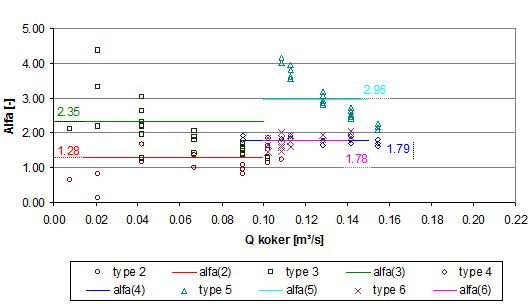
\includegraphics[width=0.95\textwidth]{graphics/culvert_fig8.png}
\end{center}
\caption{Discharge coefficient (Alfa) due to the presence of open valves for
each type of flow (source: IMDC Report 613\_9\_1)}
\label{fig:culvert_fig8}
\end{figure}

\textbf{Coefficient} $\mathbf{C_t}$\\

Trash screens are usually present at the inlet of culverts to prevent garbage
from entering or blocking the culvert. The head loss due to trash screens
($\Delta H_t$) can be estimated by its relationship with the velocity
head through the net flow area.
A number of expressions were obtained in the past by several authors.
We use the expression given by the Bureau of Reclamation \cite{Bureau1992}:
\begin{equation}
\Delta H_t = (1.45-0.45A_t-A_t^2)\dfrac{U^2}{2g} = C_t \dfrac{U^2}{2g}
\end{equation}
where $A_t=\frac{Anet}{Agross}$ gives the ratio of net flow area to gross rack area.
$U$ is the net flow velocity. The value for $C_t$ can vary between $C_t= 0$ equivalent
to not having any trash screens to approximately $C_t= 1.4$, for which the net
flow area is almost equal to the gross rack area.

Note that a very similar fomulation to this second option is included in DELFT 3D.
The main difference between the second culvert functionality in TELEMAC and the one
included in DELFT 3D is the way how the head loss coefficient is calculated.
While in TELEMAC, the Carlier reference \cite{Carlier1972} was followed, in DELFT 3D they refer
to experiments executed by Flanders Hydraulic Research.

\subsubsection{Transport of scalars through culverts}

With the implementation of the culvert functionality,
some modifications had to be done in the code such that
it would be possible to model the passage of the scalar through the culvert structure.
Following the same idea implemented to model the flow through culverts,
the concentration of the scalar in the model domain is assigned to source and sink terms
for scalars. When the flow goes from the river to the floodplain,
there is a source point in the floodplain with a scalar concentration equal to the one
in the river. At the same time in the river there is a sink term with the same scalar
concentration. The opposite happens when the flow goes from the floodplain to the river.
Please note that it is the scalar concentration that is assigned to the source term
and not the scalar concentration per second.
In its structure, TELEMAC deals with that concentration and associates it to the
discharge and volume of fluid at the source terms.
In order to take into account the transport of scalars in the model the
user has only to specify in the steering file the keywords relative to the scalars.

\subsection{Input data for \telemac{3d}}

In order to take culverts into account in \telemac{3d} the user has to define in the
steering file two keywords: \\
NUMBER OF CULVERTS \\
CULVERTS DATA FILE\\

The number of culverts has to be assigned to the keyword NUMBER OF CULVERTS
(please note that this is the number of culverts and not the number of sources/sink terms:
one culvert has two sink/source terms).
The keyword CULVERTS DATA FILE refers to an ASCII file where the geometric characteristics
and all head loss coefficients are given to be used by the code.
The text file has to follow a strict structure of the input parameters in order
for the software to read the right values for the right parameter.
Here below an example is given:\\

Relaxation, Number of culverts\\
0.05 2\\
I1  I2  CE1  CE2  CS1  CS2  LRG HAUT1 CLP LBUS Z1 Z2 CV  C56  CV5  C5 CT HAUT2 FRIC LENGTH CIRC D1  D2 A1 A2 AA\\
data culvert 1  ...\\
data culvert 2 ...\\
... \\

The index number 1 refers to the river side and the index 2 refers to the floodplain side.
I1 and I2 correspond to the index of the source/sink terms in the river side
and in the floodplain that represent the beginning and end of the culvert.
CE1, CE2 and CS1, CS2 are the head loss coefficients
for the inlet and outlet sluice entrance ($C_1$) and exit ($C_3$), respectively.
LRG represents the width of the culvert.
HAUT1 and HAUT2 the height of the culvert at the river and
floodplain side.
The flow direction is also imposed through the keyword CLP and
a relaxation parameter (variable RELAXB) is incorporated in the code.
CLP=0, flow is allowed in both directions; CLP=1, flow is only allowed from section 1 to section 2; CLP=2, flow is only allowed from section 2 to section 1; CLP=3, no flow allowed.
LBUS is the linear head loss in the culvert.
Z1 and Z2 the elevations of the culvert
extremities in the river side and in the floodplain.
CV refers to the loss coefficient due to the presence of a valve ($C_v$) and
C56 ($c$) is the constant used to differentiate flow types 5 and 6.
C5 and CV5 represent correction coefficients to C1 and to CV coefficients
due to the occurrence of the type 5 flow.
CT is the loss coefficient due to the presence of trash screens ($C_t$).
FRIC is the Manning Strikler coefficient.
The length of the culvert can be set (LENGTH parameter), and its shape can be specified through the parameter CIRC (equal to 1 in
case of a circular section, 0 for a rectangular section).
D1 and D2 are the angles that the pipe makes with respect to the bottom, in degrees.
A1 and A2 are the angles with respect to the x axis.
For a vertical intake, the angle with the bottom will therefore be 90${}^\circ$.
They are used to account for the current direction at source or sink point.
AA is a parameter which allows the user to choose whether A1 and A2 are automatically computed by TELEMAC
or whether the data file values are used to set these angles: AA=1 -- automatic angle; AA=0 -- user-set angle.
\section{\label{sec:coriolis}Coriolis%
\index{Coriolis!force}
force and centrifugal force%
\index{centrifugal force}%
}
These forces are due to the rotation of the Earth on its own axis. We
establish their expressions below. Let $\vec{k}$ be the unit vector oriented
along the rotational axis of the Earth, from South to North. The rotation
vector of the Earth can then be written as:
\begin{equation}
\vec{\Omega}=\Omega\vec{k}
\end{equation}
with $\Omega= 2\pi/T$ where $T$ is equal to $86164$: the duration in seconds of the
sidereal day.\\

Let $R_a$ be a fixed referential with its origin at the centre of the Earth and
$R_T$ a referential which turns with the Earth. In this referential, the axis $Ox$ is directed eastwards,
$Oy$ northwards and $Oz$ upwards.
For any vector $\vec{A}$, the following relation holds:
\begin{equation}
\left.\dfrac{d \vec{A}}{d t}\right|_{R_A}=\left.\dfrac{d \vec{A}}{d t}\right|_{R_T}+\vec{\Omega}\wedge\vec{A}
\end{equation}
The relation between the velocities expressed in the two referentials then reads:
\begin{equation}\label{eq:uA}
\vec{u}_{A}=\vec{u}+\vec{\Omega}\wedge\vec{r}_A
\end{equation}
which is equivalent to:%

\begin{equation}
\left(  \dfrac{d\vec{r}_A}{dt}\right)_{R_A}=\left(
\dfrac{d\vec{r}}{dt}\right)_{R_T}+\vec{\Omega
}\wedge\vec{r}_A%
\end{equation}


%This relation is a rule for time derivatives, valid for every vector with
%components in referentials $a$ and $b$. In fact, for every vector
%$\vec{i}$ of the spinning referential, $b$, we have:
%\[
%\dfrac{d\vec{i}}{dt}=\vec{\omega}\wedge\vec{i}%
%\]
By deriving $\vec{u}_{A}$ with respect to time, we get:%

\begin{equation}
\begin{array}{ll}
\left(  \dfrac{d\vec{u}_{A}}{dt}\right)_{R_A}&=\left(
\dfrac{d\vec{u}_A}{dt}\right)  _{R_T}%
+\vec{\Omega}\wedge\vec{u}_A\smallskip\\
&=\left(
\dfrac{d\vec{u}}{dt}\right)_{R_T}
+\left(\dfrac{d\vec{\Omega}}{dt}\right)_{R_T}\wedge\vec{r}
+\vec{\Omega}\wedge\left(  \dfrac
{d\vec{r}}{dt}\right)_{R_T}
+\vec{\Omega}\wedge\vec{u}
+\vec{\Omega}\wedge(\vec{\Omega}\wedge\vec{r})
\end{array}
\end{equation}
The second line is obtained by replacing $\vec{u}_A$ with its expression \eqref{eq:uA} in the first line.
The term $\left(d\vec{\Omega}/dt\right)_{R_T}$ is equal to 0 and $\left(d\vec{r}/dt\right)_{R_T}$
is equal to $\vec{u}$ by definition. We then have:
\begin{equation}
\left(  \dfrac{d\vec{u}_{A}}{dt}\right)_{R_A}=
\left(\dfrac{d\vec{u}}{dt}\right)_{R_T}
+2\vec{\Omega}\wedge\vec{u}
+\vec{\Omega}\wedge(\vec{\Omega}\wedge\vec{r})
\end{equation}
The last term of this equation is oriented along the vertical.
To write the equations of motion in the referential linked to the surface of the Earth,
it is then necessary to include the terms:
\begin{equation}
-2\,\vec{\Omega}\wedge\vec{u}%
\end{equation}
which is called the Coriolis force, as well as:
\begin{equation}
-\vec{\Omega}\wedge(\vec{\Omega}\wedge\vec{r})
\end{equation}
which is called the centrifugal force.

In the referential linked to the surface of the Earth, the vector $\vec{\Omega}$ reads:%

\begin{equation}
\vec{\Omega}=\left(
\begin{array}
[c]{c}%
\Omega_{x}\\
\Omega_{y}\\
\Omega_{z}%
\end{array}
\right)  =\left(
\begin{array}
[c]{c}%
0\\
\Omega\cos(\lambda)\\
\Omega\sin(\lambda)
\end{array}
\right)
\end{equation}
where $\lambda$ is the latitude at the considered point, counted positively
from the equator to the North pole and negatively from the equator to the South pole.
%In the more general case where north makes an angle $N$ with the axis $Oy$
%(counted positively on going from $Oy$ to the north), one has:
%\begin{equation}
%\vec{\Omega}=\left(
%\begin{array}
%[c]{c}%
%\Omega_{x}\\
%\Omega_{y}\\
%\Omega_{z}%
%\end{array}
%\right)  =\left(
%\begin{array}
%[c]{c}%
%\Omega\cos(\lambda)\sin(N)\\
%\Omega\cos(\lambda)\cos(N)\\
%\Omega\sin(\lambda)
%\end{array}
%\right)
%\end{equation}
The Coriolis force then reads:
\begin{equation}\label{eq:coriolis_complet}
-2\vec{\Omega}\wedge\vec{u}=-2\Omega\left(
\begin{array}
[c]{c}%
\cos(\lambda)w-\sin(\lambda)v\\
\sin(\lambda)u\\
\cos(\lambda)u
\end{array}
\right)
\end{equation}
The Coriolis force only has an effect on large scale flows, and is thus
usually considered in the frame of quasi-horizontal flows.
In this context, the vertical velocities are neglected. Besides,
the effect of the Coriolis force along the vertical are not taken into account
since they are negligible compared to the gravity term.
Thus, the equation \eqref{eq:coriolis_complet} becomes:
\begin{equation}\label{eq:coriolis_complet}
-2\,\vec{\Omega}\wedge\vec{u}=-2\Omega\left(
\begin{array}
[c]{c}%
-\sin(\lambda)v\\
\sin(\lambda)u\\
0
\end{array}
\right)
\end{equation}

By definition, the Coriolis coefficient%
\index{Coriolis!coefficient}
is defined by:
\begin{equation}
\gamma=2\Omega\sin(\lambda)
\end{equation}
It is about equal to $10^{-4}s^{-1}$ at
a latitude of 45$^\circ$N. The Coriolis forces have a significant impact on the
fluid motion when their magnitude is of the same order as the inertia forces.
This is measured by the Rossby number, that corresponds to the ratio between
inertia and Coriolis forces:
\begin{equation}
R_{0}=\dfrac{U}{\gamma L}%
\end{equation}
where $U$ and $L$ are characteristic horizontal velocity and length of flow. The
Coriolis force has a significant impact when $R_{0}\ge 1$; that is, for large oceanic or
atmospheric areas: for example, considering an oceanic flow with characteristic
horizontal velocity 1 m s$^{-1}$ and $\gamma$ equal to 10$^{-4}$, the Coriolis force
becomes significant for horizontal length scales larger than 10 km.
It is however negligible in rivers and lakes (and even more so in kitchen sinks...).

\begin{CommentBlock}{Remark:}
The term due to the vertical
velocity is ignored in \telemac{3d}; however, it may have some importance
in oceanic flows on the mesoscale, as pointed out by Mahadevan \textit{et al.} \cite{mahadevan96}.
\end{CommentBlock}

For a geophysical flow, the centrifugal force is not added to the
Navier--Stokes equations. In fact, one considers that the free surface of a
fluid at rest coincides with an equipotential surface of apparent gravity,
which already integrates the effect of centrifugal force.

% ---------------------------------------------------------------------------
\section{Arbitrary Lagrangian-Eulerian formulation}\label{sec:ALE}
% ---------------------------------------------------------------------------

\subsection{Principle}
The Arbitrary Lagrangian-Eulerian (ALE) formulation was developed in order to
simplify the treatment of problems with moving boundaries, in particular
for fluid-structure interaction problems and for flows with moving interfaces
(see \cite{Hirt1974, Chan1975, Donea1981}, for example). It is reviewed and interpreted
in a Finite Elements context, with a view of using it in \telemac{3d}, in \cite{Decoene2006}.
In \cite{Decoene2009}, Decoene \textit{et al.} demonstrated the equivalence between the
ALE formulation and the classical sigma-transform with a particular type of ALE mapping.
They introduced a generalised form of the sigma transformation, which can now be used in
\telemac{3d}.

The idea of the ALE formulation is to define a reference configuration -- generally chosen
to be fixed, and a mapping that gives the correspondence between the real domain and
the reference domain. The mapping can be arbitrarily chosen, but it has to
be conforming to the evolution of the domain boundaries.

The idea is then to compute the time-derivatives in the reference domain,
which is simpler than in the real (moving) domain. Indeed, in the moving domain,
the discretisation of a time derivative of a field $\vec{u}$ at position $\vec{x}$ cannot be written as:
\begin{equation}
\dfrac{\partial \vec{u}}{\partial t}(\vec{x},t) \approx \dfrac{\vec{u}(\vec{x},t^{n+1})-\vec{u}(\vec{x},t^n)}{\delta t}
\end{equation}
since $\vec{x}$ may not be in the computational domain anymore at time $t^{n+1}$.\\

Throughout this document, the reference mesh is denoted by $\Omega^*$, and
the fields in the reference mesh are denoted with a $*$ superscript.
We denote by $\mathcal{A}^*$ the mapping that associates to each point $\vec{x}^*$ in $\Omega^*$ a
point $\vec{x}$ in $\Omega$, and $\mathcal{A}$ the mapping that associates to each point $\vec{x}$ in $\Omega$ a
point $\vec{x}^*$ in $\Omega^*$. Here, we dropped the time-dependence
in the notations to simplify, but keep in mind that $\Omega$ varies in time, as well as $\mathcal{A}^*$.
$\vec{x}^*$ represents the coordinates in the reference domain.
It is assumed in \telemac{3d} that $\mathcal{A}^*$ is invertible with continuous inverse $\mathcal{A}$.

\begin{WarningBlock}{Warning:}
Note that this assumption makes it impossible for \telemac{3d} to treat the breaking
of the free-surface based on this ALE formulation.
\end{WarningBlock}

The time-derivative of a field $f$ in the reference domain is
denoted by $\left(\partial f/\partial t\right)_{x^*,y^*,z^*}(\vec{x},t)$.
In \telemac{3d} the mesh motion is only allowed along the vertical and in the
reference mesh, only the $z$ coordinate is modified.
The other coordinates and time remain unchanged. In other words, $t^{\ast}=t
$, $x^{\ast}=x$ and $y^{\ast}=y$.
The instantaneous domain velocity is defined by:
\begin{equation}\label{c_def}
\vec{c}(x,y,z^*,t)=\dfrac{\partial \mathcal{A}^*}{\partial t}
\end{equation}
Considering that, by definition of the mapping, $\vec{x}=\mathcal{A}^*(\vec{x}^*)$,
the domain velocity can also be written as follows:
\begin{equation}
\vec{c}(x,y,z^*,t)=\left(\dfrac{\partial \vec{x}}{\partial t}\right)_{x,y,z^*}=\left(\dfrac{\partial z}{\partial t}\right)_{x,y,z^*}\vec{e}_z=\left(0, 0, c\right)
\end{equation}
The Jacobian matrix of $\mathcal{A}^*$ is denoted by $\vec{J}^*$ and defined by:
\begin{equation}
J_{ij}^*(x,y,z^*,t)=\dfrac{\partial \mathcal{A}^*(x^*_i)}{\partial x^*_j}
\end{equation}
The continuous expression of the Jacobian
determinant is then:
\begin{equation}
J^*(x,y,z^*,t)=\left(\dfrac{\partial z}{\partial z^*}\right)_{x,y,t}
\end{equation}

In \telemac{3d}, the domain motion is managed through the sigma transformation,
either in its classical or its generalised form.
It is necessary here to introduce one notion of the space discretisation in
\telemac{3d}, which is that the mesh is structured on the vertical.
It is built as an extrusion of a 2D mesh along the vertical, then divided into layers.
A transformation of the variable $z$ is then done for each layer,
so that $z^*$ is equal to $0$ at the bottom of a layer and $1$ at the top.
With the generalised sigma transform, the change of variable consists in defining $z^*$ as:
\begin{align}
z^* =& \dfrac{z-z_{ip}}{z_{ip+1}-z_{ip}} = \dfrac{z-z_{ip}}{\Delta z}
\end{align}
where $z_{ip}$ is the elevation of the bottom of layer $p$ at point $i$,
$z_{ip+1}$ is the elevation of the top of layer $p$ at point $i$ and $\Delta z$ is the height of the layer $p$,
which is piecewise constant vertically.

\begin{CommentBlock}{Classical version of the sigma transformation:}
The classical sigma transformation consists in changing the vertical
coordinates so that the bed elevation becomes 0 and the free surface
elevation becomes 1. The following change of variables is then used:%
\begin{equation}
z^{\ast}=\dfrac{z-b}{\eta-b}=\dfrac{z-b}{h}%
\end{equation}
This is an affine transformation giving a transformed domain $\Omega^{*} $.
The elevations are shifted and multiplied by a coefficient $1/h$. For a
function $f$, the volume integrals are thus modified in the following manner:%
\begin{equation}
\int_{\Omega} f~d\Omega = \int_{\Omega^{\ast}}\left(\dfrac{\partial z}{\partial z^{\ast}}\right)_{x,y,t}
f^{\ast}~d\Omega^{\ast}=\int_{\Omega^{\ast}}h f^\ast ~d\Omega^{\ast}
\end{equation}
\end{CommentBlock}

From now on we shall denote the Jacobian by $\Delta z$:
\begin{equation}
J^*=\left(\dfrac{\partial z}{\partial z^{\ast}}\right)_{x,y,t}=\Delta z
\end{equation}
As a matter of fact, it will appear in the section \ref{transformation sigma}, when we deal
with the generalized sigma transformation on 3D meshes, that the Jacobian is the
local height of prisms, the depth $h$ being then the sum of these heights along the vertical.

\subsection{Writing the Navier--Stokes equations in the reference domain}
\paragraph{Space and time derivatives:}
To change referentials it is necessary to express the derivatives in the reference domain
as functions of the derivatives in the real domain.
Be careful that a partial derivative with respect to $x$ in the reference domain
implies that one derives with constant $y$, $z^{\ast}$ and $t$.
In what follows the subscripts indicate what variables remain constant in the derivation.
Then, $(\partial f/\partial x)_{y,z^*,t}$ and $(\partial f/\partial x)_{y,z,t}$ do not have the same meaning.
For space derivatives, we shall use the following basic relations:%
\begin{equation}
\left(  \dfrac{\partial f}{\partial x}\right)  _{y,z,t}\,=\,\left(
\dfrac{\partial f}{\partial x}\right)  _{y,z^{\ast},t}\,+\,\,\,\left(
\dfrac{\partial f}{\partial z^{\ast}}\right)  _{x,y,t}\,\,\left(
\dfrac{\partial z^{\ast}}{\partial x}\right)  _{y,z,t}\, \label{transfsig}%
\end{equation}
%
\begin{equation}
\left(  \dfrac{\partial f}{\partial y}\right)  _{x,z,t\,}\,=\,\left(
\dfrac{\partial f}{\partial y}\right)  _{x,z^{\ast},t\,}\,+\,\,\,\left(
\dfrac{\partial f}{\partial z^{\ast}}\right)  _{x,y,t}\,\,\left(
\dfrac{\partial z^{\ast}}{\partial y}\right)  _{x,z,t\,} \label{transfsig3}%
\end{equation}
%
\begin{equation}
\left(  \dfrac{\partial f}{\partial z}\right)  _{x,y,t\,}\,=\,\,\,\,\left(
\dfrac{\partial f}{\partial z^{\ast}}\right)  _{x,y,t\,}\,\,\left(
\dfrac{\partial z^{\ast}}{\partial z}\right)  _{x,y,t\,} \label{transfsig4}%
\end{equation}

\begin{CommentBlock}{Demonstration of the relation \eqref{transfsig}:}
\begin{align*}
\left(\dfrac{\partial f}{\partial x}\right)_{y,z,t} = &
	\left(\dfrac{\partial f}{\partial x^*}\right)_{y,z^*,t} \left(\dfrac{\partial x^*}{\partial x}\right)_{y,z,t}
	+\left(\dfrac{\partial f}{\partial y^*}\right)_{x,z^*,t} \left(\dfrac{\partial y^*}{\partial x}\right)_{y,z,t}
	+\left(\dfrac{\partial f}{\partial z^*}\right)_{x,y,t}\left(\dfrac{\partial z^*}{\partial x}\right)_{y,z,t}
\end{align*}
Since $x^* = x$ and $y^* = y$, $\left(\partial x^*/\partial x\right)_{y,z,t}=1$
and  $\left(\partial y^*/\partial x\right)_{y,z,t}=0$. Equation \eqref{transfsig} is thus obtained.
The equations \eqref{transfsig3} and \eqref{transfsig4} are obtained in the same way.
\end{CommentBlock}

Regarding the time-derivatives, the following basic formula will be used:
\begin{equation}
\left(  \dfrac{\partial f}{\partial t}\right)_{x,y,z\,}=\left(
\dfrac{\partial f}{\partial t}\right)_{x,y,z^{\ast}}+\left(
\dfrac{\partial f}{\partial z^{\ast}}\right)_{x,y,t}\left(
\dfrac{\partial z^{\ast}}{\partial t}\right)_{x,y,z} \label{transfsig2}%
\end{equation}

\begin{CommentBlock}{Remark:}
The equation \eqref{transfsig2} is equivalent to:
\begin{equation}\label{transfsig2bis}
\left(\dfrac{\partial f}{\partial t}\right)_{x,y,z^*}=\left(\dfrac{\partial f}{\partial t}\right)_{x,y,z}
+\vec{c} \cdot \Grad f
\end{equation}
which is a more  classical way to write this transport equation.
\end{CommentBlock}


By taking $f=z$ in the equations \eqref{transfsig} to \eqref{transfsig2},
and using our notation for the Jacobian, this
gives properties that will be used to write the Navier -- Stokes equations
in the reference domain:

\begin{equation}
\left(\dfrac{\partial z^{\ast}}{\partial x}\right)_{y,z,t}
=-\dfrac{1}{\Delta z}\left(\dfrac{\partial z}{\partial x}\right)
_{y,z^{\ast},t} \label{form1}%
\end{equation}
%
\begin{equation}
\left(\dfrac{\partial z^{\ast}}{\partial y}\right)_{x,z,t}
=-\dfrac{1}{\Delta z}\left(\dfrac{\partial z}{\partial y}\right)
_{x,z^{\ast},t} \label{form2}%
\end{equation}
%
\begin{equation}
\left(\dfrac{\partial z^{\ast}}{\partial t}\right)_{x,y,z}
=-\dfrac{1}{\Delta z}\left(\dfrac{\partial z}{\partial t}\right)
_{x,y,z^{\ast}} \label{form3}%
\end{equation}

Let $\vec{c}^*$ be defined by:
\begin{equation}\label{c*_def}
\vec{c}^*=\left(\dfrac{\partial z^*}{\partial t}\right)_{x,y,z}=\left(0, 0, c^*\right)
\end{equation}
$\vec{c}^*$ can be interpreted as the velocity of the reference domain.
With the definition of the domain's velocity given by \eqref{c_def}, the equation
\eqref{form3} reads:
\begin{equation}\label{velocitiesmesh}
\vec{c}+\Delta z\vec{c}^*=0
\end{equation}

The following equality holds:
\begin{equation}
\dfrac{\partial}{\partial t}\left(  \dfrac{\partial z}{\partial z^{\ast}%
}\right)_{x,y,t} = \dfrac{\partial}{\partial z^{\ast}}\left(  \dfrac{\partial
z}{\partial t}\right)_{x,y,z^*}
\end{equation}
which reads, with our notations:
\begin{equation}
\dfrac{\partial \Delta z}{\partial t} - \dfrac{\partial c_z}{\partial z^{\ast}}
= \dfrac{\partial \Delta z}{\partial t} - \Divast \vec{c} = 0
\end{equation}
Using the equation \eqref{velocitiesmesh} to replace $\vec{c}$ in the previous relation, it is equivalent to:
\begin{equation}
\dfrac{\partial \Delta z}{\partial t}+\Divast(\Delta z\vec{c}^*)=0
\end{equation}
%Using equation \eqref{velocitiesmesh} to replace $\vec{c}^*$ in the previous relation, we get:
%\begin{equation}
%\dfrac{\partial}{\partial t}\left(\dfrac{1}{\Delta z}\right)+\dfrac{\partial}{\partial
%z^{\ast}}\left(\dfrac{\vec{c}}{\Delta z}\right)=\dfrac{\partial}{\partial t}\left(\dfrac{1}{\Delta z}\right)+\Div\left(\dfrac{\vec{c}}{\Delta z}\right)=0
%\end{equation}
In the same way, we find:
\begin{equation}
\dfrac{\partial}{\partial t}\left(\dfrac{1}{\Delta z}\right)+\dfrac{\partial}{\partial
z^{\ast}}\left(\dfrac{\vec{c}}{\Delta z}\right)=\dfrac{\partial}{\partial t}\left(\dfrac{1}{\Delta z}\right)+\Div\left(\dfrac{\vec{c}}{\Delta z}\right)=0
\end{equation}

This can be interpreted as an evolution law for the Jacobian determinant.
It ensures the conservation of the domain's volume when changing referentials and will have
to be fulfilled in the discrete framework.
%With this formula and using the equation \eqref{transfsig2bis}, the following relation is obtained:
%\begin{equation}
%\dfrac{d}{dt}\int_\Omega f(\vec{x},t)~d\Omega = \int_\Omega
%\left[\left(\dfrac{\partial f}{\partial t}\right)_{x,y,z^*}+f(\vec{x},t)\Div \vec{c}\right]~d\Omega
%\end{equation}

%$\overrightarrow{W}_{mesh}$ will be the vector with components (0,0,$W_{mesh}
%$). We shall also encounter in the derivations a quantity which can be
%interpreted as the velocity of the transformed mesh:%
%
%\begin{equation}
%W_{mesh}^{\ast}=\left(  \dfrac{\partial z^{\ast}}{\partial t}\right)  _{x,y,z}%
%\end{equation}
%
%
%Equation \eqref{form3} is thus also:%
%
%\begin{equation}
%W_{mesh}+\Delta zW_{mesh}^{\ast}=0 \label{velocitiesmesh}%
%\end{equation}
%and the fact that we have:%
%
%\[
%\dfrac{\partial}{\partial t}\left(  \dfrac{\partial z}{\partial z^{\ast}%
%}\right)  -\dfrac{\partial}{\partial z^{\ast}}\left(  \dfrac{\partial
%z}{\partial t}\right)  =0
%\]
%leads to:%
%
%\[
%\dfrac{\partial(\Delta z)}{\partial t}-\dfrac{\partial(W_{mesh})}{\partial
%z^{\ast}}=\dfrac{\partial(\Delta z)}{\partial t}-div^{\ast}(\overrightarrow{W}%
%_{mesh})=0
%\]
%or:%
%
%\begin{equation}
%\dfrac{\partial(\Delta z)}{\partial t}+div^{\ast}(\Delta z\overrightarrow{W}%
%_{mesh}^{\ast})=0
%\end{equation}
%
%
%In the same way we find:%
%
%\begin{equation}
%\dfrac{\partial(\dfrac{1}{\Delta z})}{\partial t}+div\left(  \dfrac
%{\overrightarrow{W}_{mesh}}{\Delta z}\right)  =0
%\end{equation}


\paragraph{Advection terms:%
\index{advection}%
}

The advection terms must be carefully examined in a moving grid because the
advected functions vary not only under the effect of the flow, but also
because they are defined on moving points. The derivative $df/dt$,
written in the real domain, reads:%
\begin{equation}
\dfrac{df}{dt}=\dfrac{\partial f}{\partial t}
+u\dfrac{\partial f}{\partial x}
+v\dfrac{\partial f}{\partial y}
+w\dfrac{\partial f}{\partial z} \label{ugrad}%
\end{equation}
From now on, for the sake of simplicity, we drop the subscripts when the derivatives are estimated in the real domain.
Using the formula \eqref{transfsig}, this equation becomes:
\begin{equation}\label{formulaTimeDeriv}
\begin{array}{lll}
\dfrac{df}{dt} & = \dfrac{\partial f}{\partial t}
+u\left(\dfrac{\partial f}{\partial x}\right)_{y,z^*,t}
+u\dfrac{\partial f}{\partial z^{\ast}}\dfrac{\partial z^{\ast}}{\partial x}
+v\left(\dfrac{\partial f}{\partial y}\right)_{x,z^*,t}
+v\dfrac{\partial f}{\partial z^{\ast}}\dfrac{\partial z^{\ast}}{\partial y}
+w\dfrac{\partial f}{\partial z^{\ast}}\dfrac{\partial z^{\ast}}{\partial z}\bigskip\\
&=\dfrac{\partial f}{\partial t}+u\left(\dfrac{\partial f}{\partial x}\right)_{y,z^*,t}
+v\left(\dfrac{\partial f}{\partial y}\right)_{x,z^*,t}
+\left(u\dfrac{\partial z^{\ast}}{\partial x}
+v\dfrac{\partial z^{\ast}}{\partial y}
+w\dfrac{\partial z^{\ast}}{\partial z}\right)\dfrac{\partial f}{\partial z^{\ast}}
\end{array}
\end{equation}

%\begin{equation}
%\dfrac{df}{dt}=\left(\dfrac{\partial f}{\partial t}\right)_{x,y,z}%
%+u\left(\dfrac{\partial f}{\partial x}\right)_{y,z^*,t}
%+v\left(\dfrac{\partial f}{\partial y}\right)_{x,z^*,t}
%+\left(u\left(\dfrac{\partial z^{\ast}}{\partial x}\right)_{y,z,t}
%+v\left(\dfrac{\partial z^{\ast}}{\partial y}\right)_{x,z,t}
%+w\left(\dfrac{\partial z^{\ast}}{\partial z}\right)_{x,y,t}\right)\left(\dfrac{\partial f}{\partial z^{\ast}}\right)_{x,y,t}
%\end{equation}

On the other hand, the velocities in the transformed mesh are defined by:
\begin{equation}
u_{\ast}=\dfrac{dx^{\ast}}{dt}=\dfrac{dx}{dt}=u
\end{equation}
%
\begin{equation}
v^{\ast}=\dfrac{dy^{\ast}}{dt}=\dfrac{dy}{dt}=v
\end{equation}
%
\begin{equation}
w^{\ast}=\dfrac{dz^{\ast}}{dt}%
\end{equation}
The vertical velocity in the transformed mesh, $w^*$, is also equal to:%
\begin{equation}
w^{\ast}=\dfrac{\partial z^{\ast}}{\partial t}
+u\dfrac{\partial z^{\ast}}{\partial x}
+v\dfrac{\partial z^{\ast}}{\partial y}
+w\dfrac{\partial z^{\ast}}{\partial z} \label{wetoile}%
\end{equation}
The equation \eqref{formulaTimeDeriv} thus becomes:%
\begin{equation}
\dfrac{df}{dt}=\dfrac{\partial f}{\partial t}
+u\left(\dfrac{\partial f}{\partial x}\right)_{y,z^*,t}
+v\left(\dfrac{\partial f}{\partial y}\right)_{x,z^*,t}
+(w^{\ast}-c^{\ast})\dfrac{\partial f}{\partial z^{\ast}}
\label{gradstar}%
\end{equation}
When the mesh is moving, $f^{n+1}$ and $f^{n}$ correspond to points having the same $x$, $y $
and $z^{\ast}$, but not the same $z$. The partial derivatives in time in our
equations are thus expressed using $\left(\partial f/\partial t\right)_{x,y,z^{\ast}}$.
Using the equation \eqref{transfsig2}, the equation \eqref{gradstar} then becomes:%
\begin{equation}
\dfrac{df}{dt}=\left(\dfrac{\partial f}{\partial t}\right)_{x,y,z^{\ast}}
+u\left(\dfrac{\partial f}{\partial x}\right)_{y,z^*,t}
+v\left(\dfrac{\partial f}{\partial y}\right)_{x,z^*,t}
+w^{\ast}\dfrac{\partial f}{\partial z^{\ast}}
\end{equation}

Advection equations, in the transformed mesh and taking into account the
motion of the real mesh, will then have the simple form:%
\begin{equation}
\left(\dfrac{\partial f}{\partial t}\right)_{x,y,z^{\ast}}
+u\left(\dfrac{\partial f}{\partial x}\right)_{y,z^*,t}
+v\left(\dfrac{\partial f}{\partial y}\right)_{x,z^*,t}
+w^{\ast}\dfrac{\partial f}{\partial z^{\ast}}=0 \label{advectioninfixedmesh}%
\end{equation}

\begin{CommentBlock}{Equivalence between the sigma transformation and the ALE formulation}
Comparing the equations \eqref{gradstar} and \eqref{ugrad} shows that:%
\begin{equation}
u\dfrac{\partial f}{\partial x}
+v\dfrac{\partial f}{\partial y}
+w\dfrac{\partial f}{\partial z}
= u\left(\dfrac{\partial f}{\partial x}\right)_{y,z^*,t}
+v\left(\dfrac{\partial f}{\partial y}\right)_{x,z^*,t}
+(w^{\ast}-c^{\ast})\dfrac{\partial f}{\partial z^{\ast}}
\end{equation}
while the equation \eqref{velocitiesmesh}, combined with \eqref{transfsig} and \eqref{wetoile}, also yields:%
\begin{equation}
u\dfrac{\partial f}{\partial x}
+v\dfrac{\partial f}{\partial y}
+(w-c)\dfrac{\partial f}{\partial z}
=u\left(\dfrac{\partial f}{\partial x}\right)_{y,z^*,t}
+v\left(\dfrac{\partial f}{\partial y}\right)_{x,z^*,t}
+w^{\ast}\dfrac{\partial f}{\partial z^{\ast}}
\end{equation}
This shows that using the sigma transformation is equivalent to writing the equations in the ALE framework
at the continuous level. In the section \ref{sec:FS-NS}, the Navier--Stokes
equations will thus be written in the ALE framework,
using $\vec{u}-\vec{c}$ instead of $\vec{u}$ for the advection terms.
\end{CommentBlock}

\paragraph{Divergence:%
\index{divergence}%
}

We now want to write $\Div \vec{u}$ in the transformed mesh. Using
the formula \eqref{transfsig}, we have:%
\begin{equation}
\Div\vec{u}=\left(\dfrac{\partial u}{\partial x}\right)_{y,z\ast,t}
+\dfrac{\partial u}{\partial z^{\ast}}\dfrac{\partial z^{\ast}}{\partial x}
+\left(\dfrac{\partial v}{\partial y}\right)_{x,z^{\ast},t}
+\dfrac{\partial v}{\partial z^{\ast}}\dfrac{\partial z^{\ast}}{\partial x}
+\dfrac{\partial w}{\partial z^{\ast}}\dfrac{\partial z^{\ast}}{\partial z}
\end{equation}

By multiplying the previous equation by $\Delta z=(\partial z/\partial z^{\ast})_{x,y,t}$,
which depends on $x$, $y$ and $t$, but not on $z$ or $z^{\ast}$, and using the fact that:
\begin{equation}
\Delta z\left(  \dfrac{\partial u}{\partial x}\right)_{y,z^{\ast},t}=\left(
\dfrac{\partial \Delta z u}{\partial x}\right)_{y,z^{\ast},t}-u\dfrac{\partial \Delta z}{\partial x}
\end{equation}
we then get:%
\begin{equation}
\begin{array}{ll}
\Delta z\Div\vec{u} & =\left(\dfrac{\partial \Delta z u}{\partial
x}\right)_{y,z^{\ast},t}-u\dfrac{\partial \Delta z}{\partial x}+
\dfrac{\partial \Delta zu}{\partial z^{\ast}}\dfrac{\partial z^{\ast}}{\partial x}
+\left(\dfrac{\partial \Delta zv}{\partial y}\right)_{x,z^{\ast},t}\medskip \\
& -v\dfrac{\partial \Delta z}{\partial y}+
\dfrac{\partial \Delta z v}{\partial z^{\ast}}\dfrac{\partial z^{\ast}}{\partial y}
+\dfrac{\partial \Delta zw}{\partial z^{\ast}}\dfrac{\partial z^{\ast}}{\partial z} \label{toto}%
\end{array}
\end{equation}


The term $\partial \Delta zw^{\ast}/\partial z^{\ast}$ can be calculated using
the equation \eqref{wetoile}:%
\begin{equation}
\begin{array}{ll}
 \dfrac{\partial \Delta zw^{\ast}}{\partial z^{\ast}}&=
\dfrac{\partial}{\partial z^{\ast}}\left(  \Delta z\dfrac{\partial
z^{\ast}}{\partial t}\,+ \Delta zu\dfrac{\partial z^{\ast}}{\partial x}+\Delta z
v\dfrac{\partial z^{\ast}}{\partial y}+ \Delta zw\dfrac{\partial z^{\ast}%
}{\partial z}\right)\bigskip\\
&= \dfrac{\partial \Delta zu}{\partial z^{\ast}}
\dfrac{\partial z^{\ast}}{\partial x}+\dfrac{\partial \Delta zv}{\partial
z^{\ast}}\dfrac{\partial z^{\ast}}{\partial y}+
\dfrac{\partial \Delta zw}{\partial z^{\ast}}\dfrac{\partial
z^{\ast}}{\partial z}\bigskip\\
&+\Delta z\dfrac{\partial}{\partial z^{\ast}}\left(  \dfrac{\partial z^{\ast}%
}{\partial t}\right)  + \Delta zu\dfrac{\partial}{\partial z^{\ast}}\left(
\dfrac{\partial z^{\ast}}{\partial x}\right)  + \Delta zv\dfrac{\partial
}{\partial z^{\ast}}\left(  \dfrac{\partial z^{\ast}}{\partial y}\right)
+\Delta zw\dfrac{\partial}{\partial z^{\ast}}\left(  \dfrac{\partial z^{\ast}%
}{\partial z}\right)
\end{array}
\end{equation}

The equations \eqref{form1} to \eqref{form3} give:%

\begin{equation}
\dfrac{\partial}{\partial z^{\ast}}\left(  \dfrac{\partial z^{\ast}}{\partial
t}\right)  _{x,y,z}=-\dfrac{1}{\Delta z}\dfrac{\partial \Delta z}{\partial t}%
\end{equation}
%

\begin{equation}
\dfrac{\partial}{\partial z^{\ast}}\left(  \dfrac{\partial z^{\ast}}{\partial
x}\right)  _{y,z,t}=-\dfrac{1}{\Delta z}\dfrac{\partial \Delta z}{\partial x}%
\end{equation}
%

\begin{equation}
\dfrac{\partial}{\partial z^{\ast}}\left(  \dfrac{\partial z^{\ast}}{\partial
y}\right)  _{x,z,t}=-\dfrac{1}{\Delta z}\dfrac{\partial \Delta z}{\partial y}%
\end{equation}


We now assume that the Jacobian%
\index{Jacobian}
$\Delta z$ is constant vertically (which will be our case on every finite
element), and we thus have:%

\begin{equation}
\dfrac{\partial}{\partial z^{\ast}}\left(  \dfrac{\partial z^{\ast}}{\partial
z}\right)  _{x,y,t}=0
\end{equation}

\begin{WarningBlock}{Warning:}
Here the assumption of a constant Jacobian along the vertical (it will actually be constant per layer)
is strong and prevents us from using quadratic elements along the vertical of the domain.
To use such elements, it would be necessary to properly write the corresponding equation
on $(\Delta z~\Div\vec{u})$ in the reference mesh.
\end{WarningBlock}

All this leads to:%

\begin{equation}
\begin{array}{ll}
\dfrac{\partial \Delta zw^{\ast}}{\partial z^{\ast}}&=
\dfrac{\partial \Delta zu}{\partial z^{\ast}}
\dfrac{\partial z^{\ast}}{\partial x}+\dfrac{\partial\Delta
zv}{\partial z^{\ast}}\dfrac{\partial z^{\ast}}{\partial
y}+\dfrac{\partial \Delta zw}{\partial z^{\ast}}
\dfrac{\partial z^{\ast}}{\partial z}\medskip \\
&-\dfrac{\partial \Delta z}{\partial t}-u\dfrac{\partial \Delta z}{\partial
x}-v\dfrac{\partial \Delta z}{\partial y}%
\end{array}
\end{equation}
We deduce from this that:
\begin{equation}
\begin{array}{ll}
\dfrac{\partial \Delta zw}{\partial z^{\ast}}
\dfrac{\partial z^{\ast}}{\partial z}&=\dfrac{\partial \Delta zw^{\ast}%
}{\partial z^{\ast}}+\dfrac{\partial \Delta z}{\partial
t}+u\dfrac{\partial \Delta z}{\partial x}+v\dfrac{\partial \Delta z}{\partial y}\medskip \\
&-\dfrac{\partial \Delta zu}{\partial z^{\ast}}
\dfrac{\partial z^{\ast}}{\partial x}-\dfrac{\partial \Delta zv}{\partial
z^{\ast}}\dfrac{\partial z^{\ast}}{\partial y}%
\end{array}
\end{equation}


By introducing this expression into the equation \eqref{toto}, we get:

\begin{equation}
\Delta z~\Div\vec{u}=\dfrac{\partial \Delta z}{\partial t}+\left(
\dfrac{\partial \Delta zu}{\partial x}\right)  _{y,z^{\ast},t}+\left(
\dfrac{\partial \Delta zv}{\partial y}\right)  _{x,z^{\ast},t}+
\dfrac{\partial \Delta zw^{\ast}}{\partial z^{\ast}}
\label{divutransf}
\end{equation}

Other terms in the Navier--Stokes equations, such as diffusion terms, are
modified in an even more cumbersome manner.

\begin{CommentBlock}{Remark by J.-M. Hervouet:}
The numerical resolution of equations with the help of this sigma transformation is widely used but sometimes
leads to awkward numerical artefacts (creeping diffusion etc.). We shall try
to avoid this wherever possible, in particular during the diffusion stage.
\end{CommentBlock}


% ---------------------------------------------------------------------------
\section{Final set of equations}\label{sec:FS-NS}
% ---------------------------------------------------------------------------

\subsection{Navier--Stokes equations in Cartesian coordinates}

The Navier-Stokes equations are now written as follows, in the ALE framework,
with the decomposition of $p$ into $p_h$ and $p_d$ and where $\rho$ is constant, equal to $\rho_0$:
\begin{equation}
\left\{\begin{array}{l}
  \displaystyle{\dfrac{\partial \vec{u} }{\partial t} + ((\vec{u}-\vec{c}) \cdot \Grad) \vec{u} = -\dfrac{1}{\rho} \Grad (p_h+p_d) + \dfrac{1}{\rho} \BDiv \left(\mu_E \Grad \vec{u}\right)+ \vec{g} + \vec{F}}\medskip\\
  \displaystyle{p_h = g\rho(\eta-z) + p_{atm} + g\rho\int_z^\eta\dfrac{\Delta\rho}{\rho}~dz}\medskip\\
  \displaystyle{\dfrac{\partial\eta}{\partial t}
  + \DivD\left(\int_b^\eta\vec{u}_{2D}~dz\right) = F_b} \medskip \\
  \displaystyle{\Div \vec{u} = 0}
  \label{eq:NS_FS}
\end{array}\right.
\end{equation}
Here we wrote the system in the real domain $\Omega$ but without specifying any time-evolution of the domain yet, otherwise
the notations would be much more complex. Bear in mind that in the chapter \ref{Chapter4}, we will
write the space-time discretisation of this system, written in a moving domain.
From now on we define:
\begin{align}
  \vec{F}^{visc}= \dfrac{1}{\rho} \vec{\Div} \left(\mu_E \Grad \vec{u}\right)
  \label{eq:visc_forces}
\end{align}

Let us expand the system of equations \eqref{eq:NS_FS} in order to seperate the horizontal components and the vertical components:

\begin{equation}
  \left\{\begin{array}{l}
    \displaystyle{\dfrac{\partial u}{\partial t} = - ((\vec{u}-\vec{c})\cdot\Grad)u + F_x^{visc} - g\dfrac{\partial\eta}{\partial x} - \dfrac{1}{\rho}\dfrac{\partial p_d}{\partial x} + \tilde{F}_x}
    \notag \medskip\\
    \displaystyle{\dfrac{\partial v}{\partial t} = - ((\vec{u}-\vec{c})\cdot\Grad)v + F_y^{visc} - g\dfrac{\partial\eta}{\partial y} - \dfrac{1}{\rho}\dfrac{\partial p_d}{\partial y} + \tilde{F}_y}
    \notag \medskip\\
    \displaystyle{\dfrac{\partial w}{\partial t} = - ((\vec{u}-\vec{c})\cdot\Grad)w + F_z^{visc} - \dfrac{1}{\rho}\dfrac{\partial p_d}{\partial z} + F_z}
    \notag \medskip\\
    \displaystyle{p_h = g\rho(\eta-z) + p_{atm} + g\rho\int_z^\eta\dfrac{\Delta\rho}{\rho}~dz}\medskip\\
    \displaystyle{\dfrac{\partial\eta}{\partial t} = - \DivD\left(\int_b^\eta\vec{u}_{2D}~dz\right)+ F_b}
    \notag \medskip\\
    \displaystyle{\Div\vec{u} = 0}
  \end{array}\right.
  \label{eq:NS_FS_expanded}
\end{equation}

where the buoyancy terms are included in $\tilde{F}_x$ and $\tilde{F}_y$ (see the section \ref{sec:boussinesq}). Besides this system of equations, we also solve
a scalar equation:
\begin{equation}
\dfrac{\partial T}{\partial t}+\left((\vec{u}-\vec{c})\cdot\Grad\right)T - \Div\left(K_{E}\Grad T\right)+Q=0
\label{eq:scalarEquation}
\end{equation}

\subsection{Navier--Stokes equations in Mercator projection%
  \index{Mercator projection}}

Storm surges and storm-induced currents, differences between the actual levels
of the sea and currents and their values if the tides alone were considered,
are due to the variations of atmospheric pressure and the effect of the wind
on large stretches of the ocean. To carry out numerical simulations, vast
maritime areas are discretised on the basis of maps which are Mercator
projections of portions of the Earth's sphere. It is then necessary to find
out how this Mercator projection modifies the Navier--Stokes equations.

The Mercator projection belongs to the family of conformal projections which
ensure the local conservation of angles, but not distances. In other words,
the scale of the map is not the same at every point, but at a given point the
scale is the same in all directions. The domain to be represented in plane
form is on the surface of a sphere, whose points are identified by their
latitude $\lambda$ and their longitude $\varphi$ (see the figure \ref{figure4}).
Henceforth, it is assumed that the latitude and longitude are angles expressed
in radians, counted positively in the northern hemisphere and to the east of
the Greenwich Meridian and negatively otherwise.%

\begin{figure}[tbh]%
  \centering
  \includegraphics[scale=0.3]%
  {graphics/spherical_coordinates.pdf}%
  \caption{Definition of the longitude $\varphi$ and latitude $\lambda$ (the figure is taken from \cite{hervouet007},
  figure 2.4).}%
  \label{figure4}%
\end{figure}

On the basis of a sphere, we arrive at a plane called the Mercator plane, with
the help of the projection, which to any point $M$ of the sphere associates a
point $M_{p}$ of a cylinder tangent to the Earth at the equator (see the figure
\ref{figure5}).%

\begin{figure}[tbh]%
  \centering
  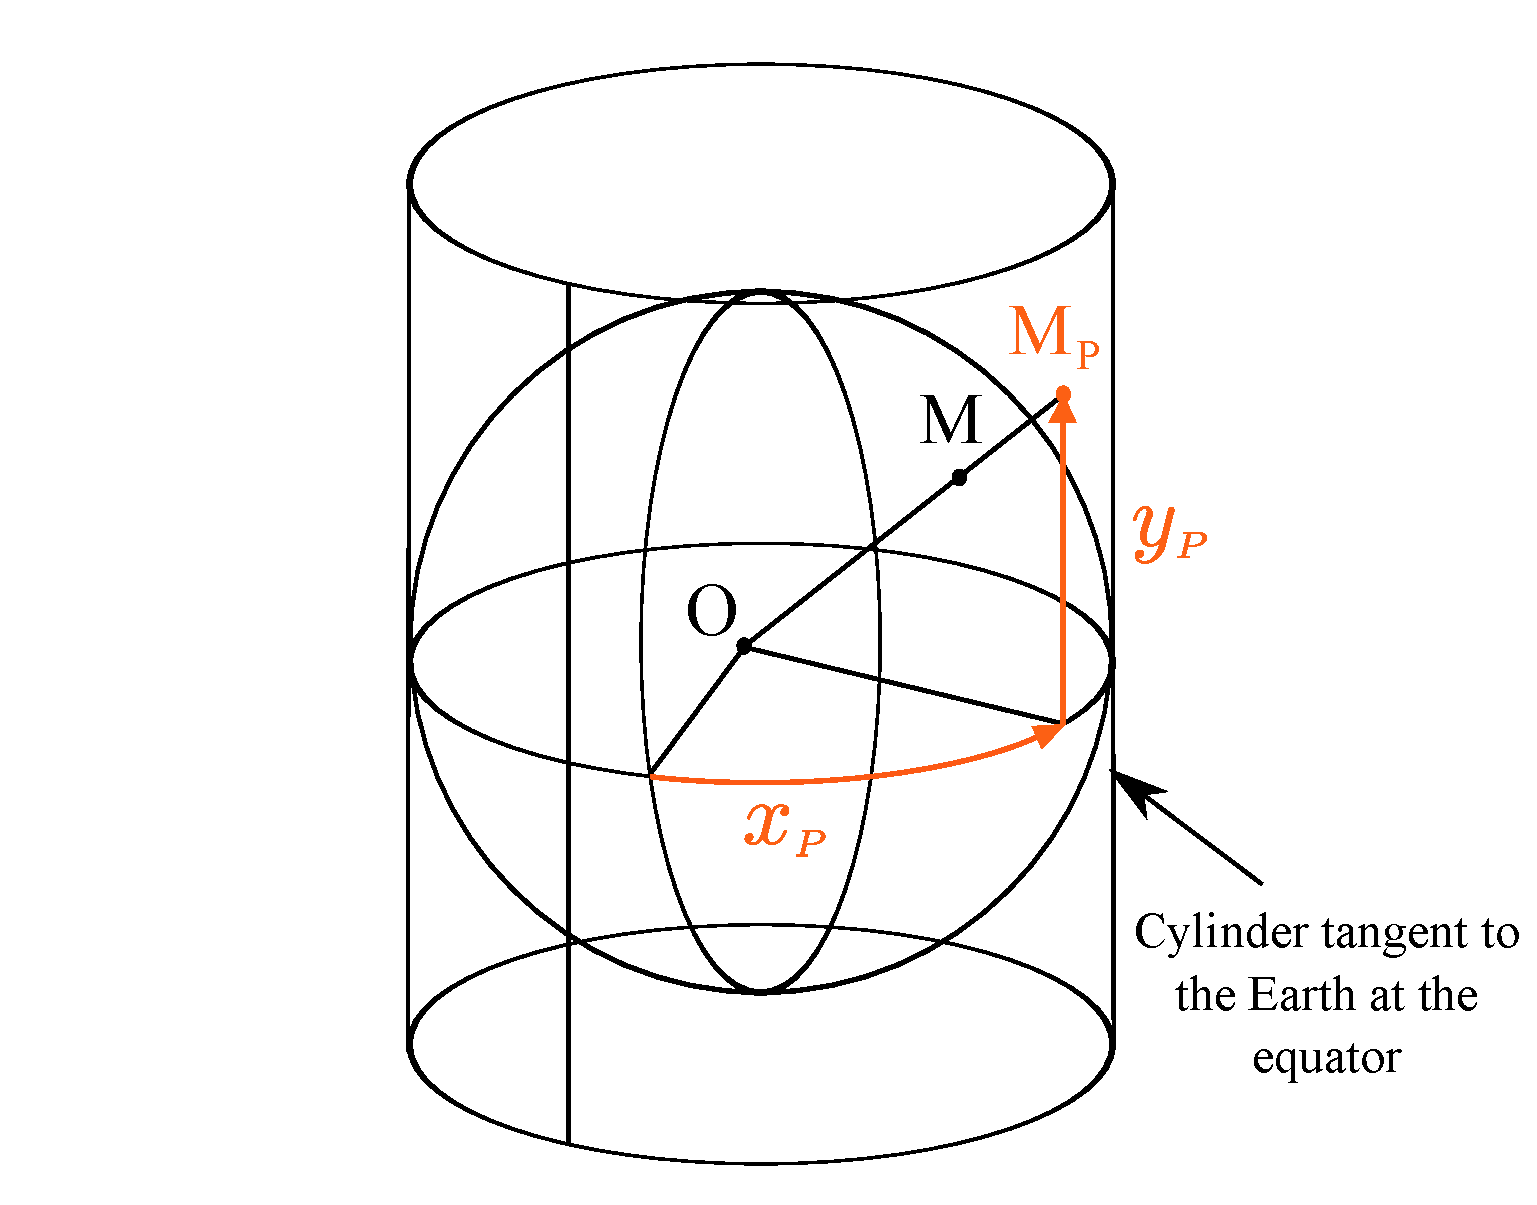
\includegraphics[scale=0.4]
  {graphics/mercator.pdf}%
  \caption{Sketch of the first phase of the Mercator projection (this figure is
  inspired by the figure 2.5 in \cite{hervouet007}).}%
  \label{figure5}%
\end{figure}
% EndExpansion

The coordinates $x_{p}$ and $y_{p}$ on this plane are deduced from the
geographical coordinates by:%
\[x_{p}=R\,\varphi\]
\[y_{p}=R\tan(\lambda)\]
However, the coordinates written in this referential do not correspond to a
conformal projection because:

\begin{itemize}
\item for an east--west displacement, $dx$, on the surface of the Earth, we
  obtain a displacement $dx_{p}$ in this referential such as:
\end{itemize}
\begin{equation}
  dx=\cos(\lambda)\,dx_{p}%
\end{equation}
\begin{itemize}
\item while for a north--south displacement, $dy$, we obtain a displacement
  $dy_{p}$ such as:
\end{itemize}
\begin{equation}
  dy=\cos^{2}(\lambda)\,dy_{p}%
\end{equation}

This distortion, which is greater in the north--south direction than in the
east--west direction, makes the projection non-conformal. We get a conformal
projection by a simple change of scale in the $y$ direction. The new ordinate
$Y$ is then deduced from $y_{p}$, then from $\lambda$, by:%
\begin{equation}
  dY=\cos(\lambda)\,dy_{p}=\dfrac{R}{\cos(\lambda)}d\lambda
\end{equation}
Moreover, it is possible to carry out a change in the origin at one point
$(\varphi_{0},\lambda_{0})$. Along the horizontal axis we immediately obtain:%
\begin{equation}
  X=R(\varphi-\varphi_{0})
\end{equation}
Along the vertical axis, we obtain by integration:%
\begin{equation}
  Y=R\left(  \ln\left[  \tan\left(  \dfrac{\lambda}{2}+\dfrac{\pi}{4}\right)
    \right]  -\ln\left[  \tan\left(  \dfrac{\lambda_{0}}{2}+\dfrac{\pi}{4}\right)
    \right]  \right)
\end{equation}
These coordinates $X$ and $Y$ are coordinates taken on maps and input to the
software for numerical simulation. Hence, one should know how to express the
Navier--Stokes equations in these coordinates. $X$ and $Y$ being functions of
spherical coordinates, it is therefore practical to express the equations in
these spherical coordinates at the very beginning. For this, we use the
divergence and gradient operators expressed in these coordinates:%
\begin{equation}
  \Div \vec{F}=\dfrac{1}{R\cos(\lambda)}\dfrac{\partial F_{\varphi}}%
  {\partial\varphi}+\dfrac{1}{R\cos(\lambda)}\dfrac{\partial(F_{\lambda}%
    \cos(\lambda))}{\partial\lambda}%
\end{equation}
%
\begin{equation}
  \vec{grad}(f)=\dfrac{1}{R\cos(\lambda)}\dfrac{\partial f}%
  {\partial\varphi}\vec{e}_{\varphi}+\dfrac{1}{R}\dfrac{\partial f}{\partial
    \lambda}\vec{e}_{\lambda}%
\end{equation}

Given the nature of the physical quantities and of the projection, the scalar
and vectorial quantities (depth, velocity) are unchanged. We have for example
$F_{\varphi}=F_{x}$ and $F_{\lambda}=F_{y}$.
The derivatives of the functions with respect to $\varphi$ and $\lambda$ are
then replaced by the derivatives along $X$ and $Y$, the Mercator coordinates:%
\begin{equation}
  \dfrac{\partial f}{\partial\varphi}=\dfrac{\partial f}{\partial X}\dfrac{\partial
    X}{\partial\varphi}+\dfrac{\partial f}{\partial Y}\dfrac{\partial Y}%
  {\partial\varphi}=R\dfrac{\partial f}{\partial X}%
\end{equation}
%
\begin{equation}
  \dfrac{\partial f}{\partial\lambda}=\dfrac{\partial f}{\partial X}\dfrac{\partial
    X}{\partial\lambda}+\dfrac{\partial f}{\partial Y}\dfrac{\partial Y}%
  {\partial\lambda}=\dfrac{R}{\cos(\lambda)}\dfrac{\partial f}{\partial Y}%
\end{equation}

From this, new expressions of divergence%
\index{divergence}
and gradient%
\index{gradient}
are deduced:%
\begin{align}
  \Div \vec{F}  &  =\dfrac{1}{\cos(\lambda)}\dfrac{\partial F_{x}}{\partial
    X}+\dfrac{1}{\cos(\lambda)}\dfrac{\partial F_{y}}{\partial Y}-\dfrac{\tan
    (\lambda)}{R}F_{y}\nonumber\\
  &  =\dfrac{1}{\cos^{2}(\lambda)}\dfrac{\partial}{\partial X}(F_{x}\cos
  (\lambda))+\dfrac{1}{\cos^{2}(\lambda)}\dfrac{\partial}{\partial Y}(F_{y}%
  \cos(\lambda))
\end{align}
%
\begin{equation}
  \Grad(f)=\dfrac{1}{\cos(\lambda)}\left(
    \begin{array}
      [c]{c}%
      \dfrac{\partial f}{\partial X}\\
      \dfrac{\partial f}{\partial Y}%
    \end{array}
  \right)
\end{equation}
The equations could be solved by using all these formulae, but, in finite
elements, this would induce a problem with the approximation space. As a matter
of fact, if $\lambda$ is a polynomial function, what becomes of $\cos
(\lambda)$? If $\cos(\lambda)$ and $\sin(\lambda)$ are polynomials, what is
$\tan(\lambda)$? These questions are fundamental when mass conservation has to
be proved.

Now,\ if we take \textit{e.g.} a conservative advection equation:%
\begin{equation}
  \dfrac{\partial f}{\partial t}+\Div(f\,\vec{u})=0
\end{equation}
it becomes in Mercator projection:%
\begin{equation}
  \dfrac{\partial(f\cos^{2}(\lambda))}{\partial t}+\Div(\cos(\lambda)f\,\vec{u})=0
\end{equation}
where $\Div$ is now the Cartesian divergence operator.
We shall see that integration into the Mercator domain of this equation will
give terms such as:%
\[\dfrac{\partial}{\partial t}\int\nolimits_{\Omega}f\cos^{2}(\lambda
)\,dXdY\,\,\text{\thinspace\ and}\,\,\,\,\int\nolimits_{\Omega}\Div(f\,\vec
{u}\cos(\lambda)\,)\,dXdY\,\,\]
this last term being equal to:%
\[\,\int\nolimits_{\Gamma}f\,\vec{u}\,.\,\vec{n}\,\cos(\lambda)\,d\Gamma\]
In these terms, each length $dX$, $dY$ or $d\Gamma$\ is multiplied by
$\cos(\lambda)$, which restores a real local scale. The volumes or flux
calculated are thus real quantities. In the same way, the gradient terms would
give real slopes.
As in the case of all operators, the coordinates therefore appear multiplied
by $\cos(\lambda)$. The idea is to carry out this operation once and for all
before the start of calculations. This can be formalised by choosing a
constant latitude $\lambda$ per element. The advantage is that the equations
to be worked out are then strictly identical to the Cartesian equations (this
is actually due to the local character of the operators and is not a general
property). This choice of constant latitude per element is naturally an
approximation, but it enables us to retain strict finite element formalism,
the approximation being somehow transferred to the coordinates.
During a computation using spherical coordinates with a meshing in the
Mercator projection, we shall build up a set of coordinates multiplied by
$\cos(\lambda)$. If we use the coordinates modified in this manner, the
Mercator projection is naturally taken into consideration and no other
modification appears again in the Navier-Stokes equations. All the mass and
flow calculations are coherent and provide real values.
The error in taking a constant latitude per element can be evaluated by
finding the form which the Navier-Stokes equations should take with the
coordinates $X^{\prime}$ and $Y^{\prime}$ such as $X^{\prime}=X\,\cos
(\lambda)$ and $Y^{\prime}=Y\,\cos(\lambda)$. The difference at the continuum
level between the equations makes the ignored terms, which are of the order of
$1/R$, appear. They take into consideration the variations in latitude within
the element.

\begin{CommentBlock}{Important note by J.-M. Hervouet:}
  The multiplication of coordinates of the points by the cosine of a
  constant latitude per element leads to a paradoxical situation: a point which
  belongs to several elements has as many sets of different coordinates which
  should be stored element by element. In fact this does not constitute a technical
  problem and does not lead to any contradiction. All calculations of vectors or
  matrices in finite elements start at the elementary level, where coherence is
  required only between the coordinates of the points of the element. It should
  even be possible, without any topological problem, to build a
  \textquotedblleft two-dimensional\textquotedblright\ meshing of the Earth for
  calculating world tides, each element having coordinates corresponding to a
  local projection (the poles should be excluded, however, having infinite coordinates
  in Mercator projection).
\end{CommentBlock}

\newpage

\chapter{Principles of the Finite Elements method}\label{Chapter2}
\section{Introduction}

A very simple description of the Finite Elements method is given here. It might require
further development, but a list of reference works is given if more details
are needed. In particular, we recommend the book by Ern \& Guermond \cite{Ern2004}.

%The finite element method is based on two ideas: an interpolation
%method and a variational method known as \textquotedblleft weighted
%residuals\textquotedblright. Each of these methods has a similar aim: to pass
%from a continuous problem to a discrete problem. If a function $u$ is defined
%by the equation $L(u)=0$ on a continuous domain $\Omega$, the interpolation
%method will provide an approximate function of$\ u$ constructed from a finite
%number of real numbers. The variational method will replace the continuous
%equation $L(u)=0$, valid at every point of $\Omega$, by a finite number of
%equations. In short, interpolation discretizes the unknown and the variational
%principle discretizes the equation. This should be specified in a strict
%mathematical framework, which (sometimes) helps to show the existence and
%uniqueness of the solution. Unfortunately, in free surface fluid mechanics,
%these demonstrations only exist in simple cases.

The domain of computation $\Omega$ is an open and bounded domain in $\mathbb{R}^{N}$,
$\mathbb{R}$ being the set of real numbers.
$N$ is the space dimension, equal to 3 in TELEMAC-3D.
$\Gamma$ is the boundary, regular (a normal vector can be defined on it),
of $\Omega$. At the continuum level, physical quantities (pressure,
temperature, components of the velocity vector, etc.) are functions of
$\Omega$ in $\mathbb{R}$. Moreover, we require that these functions are square integrable and
$L^{2}(\Omega)$ denotes the set of square integrable functions. A dot product
can be defined on this set as:%

\begin{equation}
(u,v)_{0}=\int_{\Omega}uv~d\Omega
\end{equation}


A subset of $L^{2}(\Omega)$ is composed of functions whose derivatives along
the $N$ directions of space are also square integrable. This guarantees that a
function gradient would also be square integrable. This subset is denoted
$H^{1}(\Omega)$. A new dot product is defined in $H^{1}(\Omega)$ as:%

\begin{equation}
(u,v)_{1}=\int_{\Omega}uv+\overrightarrow{grad}(u)\cdot\overrightarrow{grad}%
(v)~d\Omega
\end{equation}


The spaces $L^{2}(\Omega)$ and $H^{1}(\Omega)$ with their dot product are
called Hilbert%
\index{Hilbert space}
spaces. Hilbert spaces are very similar to the Euclidean vector spaces. On
both of them, and with the help of the dot product, we can define:
\begin{itemize}
\item a norm:%
  \begin{equation}
    \left\|  u\right\|  =\sqrt{(u,u)}%
  \end{equation}
\item a distance:%
  \begin{equation}
    d(u,v)=\left\|  u-v\right\|
  \end{equation}
\item and an angle:%
  \begin{equation}
    \cos(\alpha)=\frac{(u,v)}{\left\Vert u\right\Vert \left\Vert v\right\Vert }%
  \end{equation}
\end{itemize}
but their dimension is infinite. $H^{1}(\Omega)$ has been described with
derivatives of the first order. $H^{k}(\Omega)$ can be described in the same
way, with derivatives of the $k$th order, like the set of functions whose
derivatives up to $k$th order are all square integrable. The $H^{k}(\Omega)$
spaces are known as Sobolev%
\index{Sobolev space}
spaces.

As for the equations being worked out, only linear equations with partial
derivatives are considered (fluid mechanics equations are generally
non-linear, but the resolution methods used for solving them will generally be
written in a linear form). Here are some of the linear equations that we shall
come across later:

Helmholtz equation:%
\index{Helmholtz equation}%
%

\begin{equation}
\frac{\partial^{2}u}{\partial x^{2}}+\frac{\partial^{2}u}{\partial y^{2}%
}+\lambda u=0
\end{equation}


Poisson equation:%
\index{Poisson equation}%
%

\begin{equation}
\frac{\partial^{2}u}{\partial x^{2}}+\frac{\partial^{2}u}{\partial y^{2}}=f
\end{equation}


In this chapter, we consider that our equation is in the form:%

\begin{equation}
L(u)=f
\end{equation}


Interpolation and the variational method will now be described more precisely.


\section{Interpolation in finite elements}

The general idea is to replace an unknown function $u$, which belongs to an
infinite dimensional space, by an approximation $u_{h}$ defined on a finite
dimensional space $N$. This is an approximation and we cannot always ensure
that $L(u_{h})=f$. We simply try to minimize $L(u_{h})-f$ and this will be the
goal of the variational method.

In finite elements, a function $u$ is represented by $n$ real numbers which
are the exact values of $u$ at special points of the domain known as degrees
of freedom. For the other points, an interpolation is sufficient. To define a
unique interpolation function, e.g. a polynomial one, with exact values of $u$
for the $n$ degrees of freedom would be very complex, or would lead at least
to a high-order function. So, finite elements give up the univocal nature of
the interpolation function and choose a locally simple interpolation function
(e.g. constant, linear, quadratic). A tessellation of space into segments,
triangles, quadrilaterals, tetrahedra, prisms, etc., is executed. The degrees
of freedom are assigned to these elements, on the vertices, at the centre of
gravity, in the middle of the sides, etc., for example. Thus, each element is
described both by the coordinates of its geometric nodes and by those of its
interpolation nodes. This is followed by a simple definition of interpolation
within each element. For example, in one dimension, taking the vertices of
segments as degrees of freedom, a linear interpolation will be chosen. The
function $u_{h}$ approximating $u$ can then be written as:%

\begin{equation}
u_{h}=\sum\limits_{i=1}^{n}u_{i}\Psi_{i}%
\end{equation}
where $\Psi_{i}$ is a basis function defined differently, but in a linear
manner, on each segment ending at the point $i$. Outside these segments,
$\Psi_{i}$ is zero. Figure \ref{base en 1D} shows this basis function in one
dimension, on a non-regular mesh. The value of $\Psi_{i}$ is 1 at point i, and
0 on all the other degrees of freedom.%

\begin{figure}[H]%
\centering
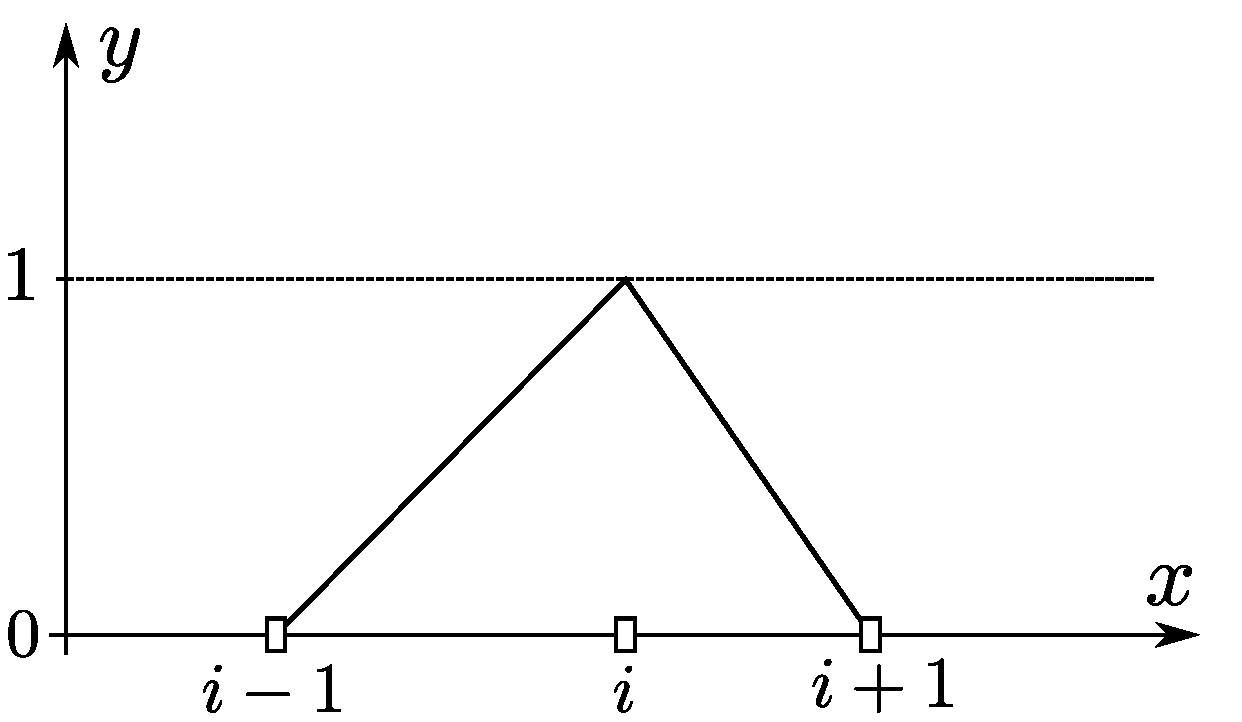
\includegraphics[scale=0.4]
{graphics/linear_basis_1D.pdf}
\caption{Shape of a linear basis in one dimension.}%
\label{base en 1D}%
\end{figure}


The property $\sum\nolimits_{i=1}^{n}\Psi_{i}=1$ is very important and will be
the key to several demonstrations. In two dimensions, with triangles and a
linear interpolation, each basis $\Psi_{i}(x,y)$ will be written as $ax+by+c$,
$a$, $b$ and $c$ depending on the triangle, so as to obtain the value 1 at
point $i$ and 0 at the other ones. Figure \ref{emprise base} shows the extent
and the nodal values of a linear basis on a finite element mesh.%

\begin{figure}[H]%
\centering
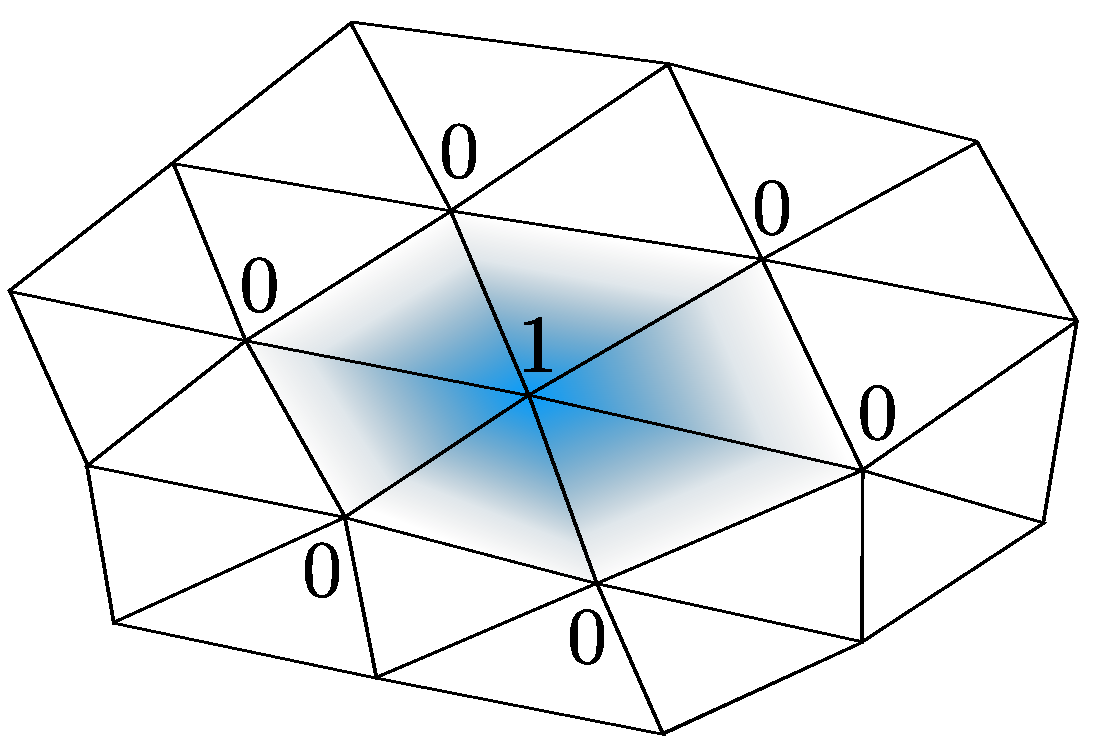
\includegraphics[scale=0.4]
{graphics/linear_basis_2D.pdf}%
\caption{Extent of a basis function on a triangular mesh. The blue color represents higher values of the basis function.}%
\label{emprise base}%
\end{figure}

These basis functions are sometimes called \textquotedblleft shape
functions\textquotedblright. With a linear interpolation, a linear function
$u$ will be represented exactly. It is said to be in the approximation space.
The interpolation can also be quadratic, or of any other order which enables
representation of the function on the degrees of freedom but also some of its derivatives.
Sometimes, and it is so for quadrilaterals, the element is too complex to get
a simple definition of the interpolation. So, we go back to a more regular
reference element (a square in the case of a quadrilateral) in a
\textquotedblleft reference\textquotedblright\ space and define a geometric
transformation between the two spaces. Interpolation is simple only in the
reference space, except in the case of simplicial elements: segments,
triangles and tetrahedra with linear interpolation. The description of
different finite elements and the use of a reference space for building finite
element matrices are explained in Reference \cite{hervouet007}. A precise
description of a large number of other elements can also be found in reference
\cite{dhatt81}.\\

%\subsection{The finite elements used in TELEMAC-3D}
In TELEMAC-3D, Lagarange finite elements are used: P1 bases on prismatic
3D elements. The bases we use can be decomposed into the poduct of
2D basis with vertical bases:
\begin{equation}
\Psi=\Psi^H\Psi^V
\end{equation}
with:
\begin{equation}
\dsum_{i=1}^{n}\Psi_i=1~,~~\dsum_{i=1}^{npoin2}\Psi_i^H=1~,~~\dsum_{i=1}^{nplan}\Psi_i^V=1
\end{equation}
where $npoin2$ is the number of points of the 2D mesh, $nplan$ is the number of
points along the vertical, $\Psi^H$ is represented in the figure \ref{emprise base} and $\Psi^V$ is
a 1-D P1 basis along $z$, as represented in the figure \ref{base en 1D}, but defined on the quadrangles composing the lateral faces of the prisms.
In order to simplify the computations of the matrices stemming from the Finite Eelements formulations, 
they are calculated in reference elements and with reference bases. 
Each element of the real mesh is transformed into a reference element, and the elementary
contributions are computed in each element in a decoupled way. In TELEMAC-3D, the
Edge-by-Edge technique is applied and there is no global matrix assembly. 
%The diagonal and extra-diagonal terms of the matrices are stored separately 
%and vectorised procedures for performing algebraic operations are provided.
The reference element used in TELEMAC-3D is shown in the figure \ref{fig:reference_element}. 

\begin{figure}
\begin{center}
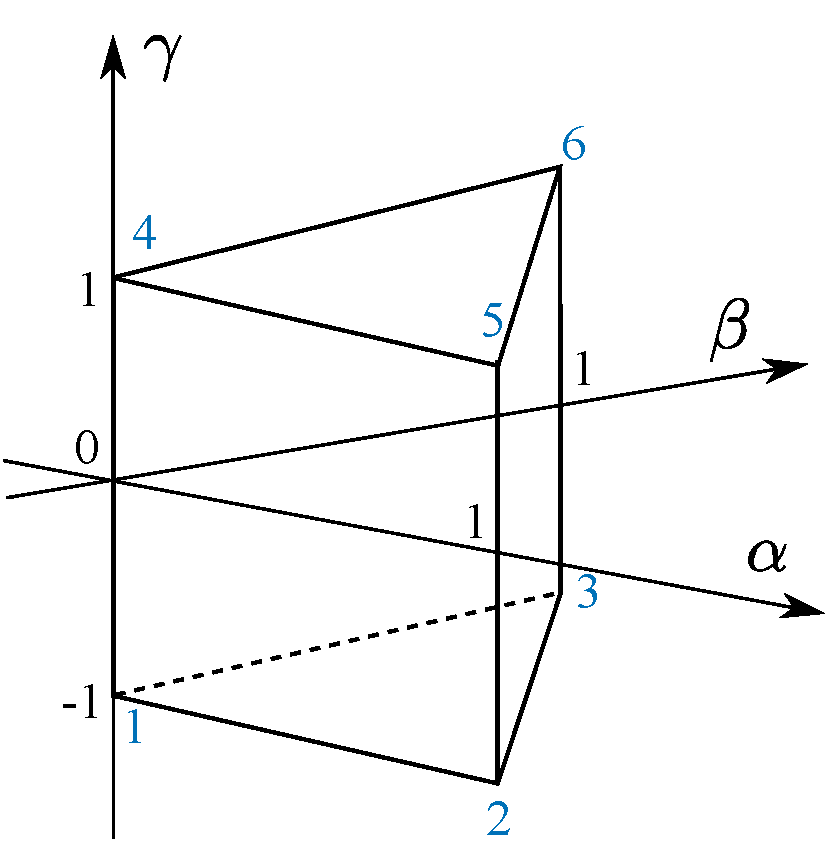
\includegraphics[scale=0.5]{./graphics/reference_element.pdf}
\end{center}
\caption{Sketch of the reference element used in TELEMAC-3D. The nodes indices
are indicated in blue whereas the coordinates in the $(\alpha, \beta, \gamma)$
system are indicated in black.}
\label{fig:reference_element}
\end{figure}

The basis functions $\Phi_i$ corresponding to the 6 nodes of the reference element read:
\begin{equation}
\begin{array}{ll}
\Phi_1 = (1-\alpha-\beta)(1-\gamma)/2 \hspace{0.5cm}& \Phi_4 = (1 - \alpha - \beta)(1 + \gamma)/2 \medskip \\
\Phi_2 = \alpha(1 - \gamma)/2 &\Phi_5 = \alpha(1 + \gamma)/2 \medskip \\
\Phi_3 = \beta(1 - \gamma)/2 &\Phi_6 = \beta(1 + \gamma)/2
\end{array}
\end{equation}

The basis functions $\Psi_i$ in the real mesh are obtained by an 
iso-parametric transformation of $\Phi_i$. The nodes of the prismatic elements 
in the real mesh have coordinates $(x_i, y_i, z_i)$. 
The coordinates of a point $P(x, y, z)$ within an element of the real mesh
are related to the coordinates in the reference element by:
\begin{equation}
x=\sum_{i=1}^6x_i\Phi_i(\alpha,\beta,\gamma)~,~~~y=\sum_{i=1}^6y_i\Phi_i(\alpha,\beta,\gamma)~,~~~z=\sum_{i=1}^6z_i\Phi_i(\alpha,\beta,\gamma)
\label{eq:xprism}
\end{equation}
Since the lateral faces of the prisms are vertical, some coordinates coincide: 
$x_1=x_4$, $y_1=y_4$, $x_2=x_5$, $y_2=y_5$, $x_3=x_6$, $y_3=y_6$, so that the
relations \eqref{eq:xprism} are simplified into:
\begin{equation}
\begin{array}{l}
x = (1-\alpha-\beta)x_1+\alpha x_2+\beta x_3 \medskip\\
y = (1-\alpha-\beta)y_1+\alpha y_2+\beta y_3 \medskip\\
z = \dfrac{1}{2}\left[(1-\alpha-\beta)z_1+\alpha z_2+\beta z_3\right](1-\gamma)+
 \dfrac{1}{2}\left[(1-\alpha-\beta)z_4+\alpha z_5+\beta z_6\right](1+\gamma)
\end{array}
\end{equation}
The Jacobian of this transformation, denoted by $|\vec{J}|$, reads:
\begin{equation}
\begin{array}{ll}
|\vec{J}|& =\dfrac{1}{2}\left[(x_2-x_1)(y_3-y_1)+(x_1-x_3)(y_2-y_1)\right]\medskip \\
& \left[(1-\alpha-\beta)z_4+\alpha z_5+\beta z_6-(1-\alpha-\beta)z_1-\alpha z_2
-\beta z_3\right]
\end{array}
\label{eq:jacobian}
\end{equation}
Let $F$ be the transformation that from $(\alpha, \beta, \gamma)$ 
yields $(x,y,z)$. The bases in the real mesh $\Psi_i$ are obtained 
from the bases in the reference element through:
\begin{equation}
\Psi_i(x,y,z)=\Phi_i(F^{-1}(x,y,z))
\label{eq:transfF}
\end{equation}

In some parts of the algorithm a two-dimensional approach is needed, 
as \textit{e.g.} in the free-surface step or for the computation of the 
friction in the diffusion step. In the case of the 2-D integrals, triangular 
elements with linear interpolation are used. For vertical lateral boundaries, 
quadrilaterals with linear interpolation are used. 
The reference elements are: a triangle with nodes at $(0, 0)$, $(0, 1)$, $(1, 0)$ and a square with nodes $(-1,-1)$, $(1,-1)$, $(1, 1)$, $(-1, 1)$, as 
represented in the figure \ref{fig:reference_elements_2D}.
The linear interpolation functions for the triangle are:
\begin{equation}
\Phi_1 = (1 - \xi - \lambda)
\Phi_2 = \xi
\Phi_3 = \lambda
\end{equation}
and for the quadrilaterals:
\begin{equation}
\Phi_1 = (1 - \xi - \lambda + \xi\lambda)/4
\Phi_2 = (1 + \xi - \lambda - \xi\lambda/4
\Phi_3 = (1 + \xi + \lambda + \xi\lambda)/4
\Phi_4 = (1 - \xi + \lambda - \xi\lambda)/4
\end{equation}
\begin{figure}
\begin{center}
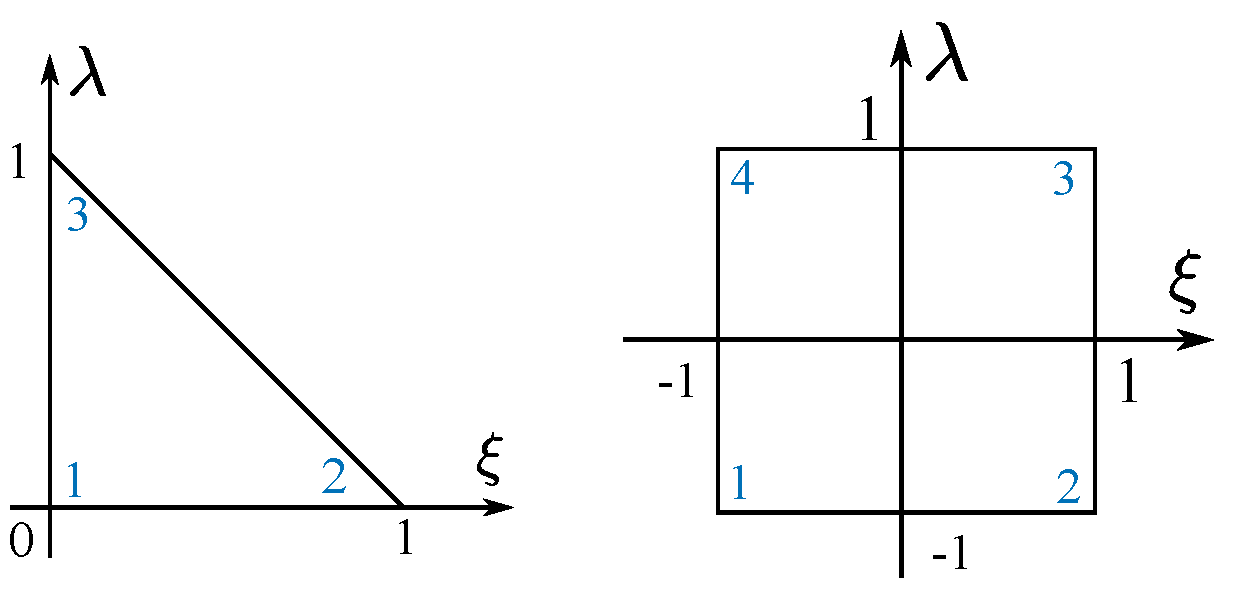
\includegraphics[scale=0.5]{./graphics/reference_elements_2D.pdf}
\end{center}
\caption{Sketch of the 2D reference elements used in TELEMAC-3D. 
The nodes indices are indicated in blue whereas the coordinates in the
local referential of each element are indicated in black.}
\label{fig:reference_elements_2D}
\end{figure}

\section{Variational principle for boundary value problems%
\index{variational formulation}%
}

Having restricted our function $u$ to a representation $u_{h}$, based on a
discrete number of unknowns $u_{i}$, we now wish to minimize $L(u_{h})-f$. The
variational method states that the dot product
$\int_{\Omega}(L(u_{h})-f)\varphi_{i}~d\Omega$
is zero for some functions $\varphi_{i}$ called test
functions\index{test function}.
The choice of these functions defines the variants of the finite element
method. The most classical technique, the Galerkin technique, consists in
choosing test functions equal to the basis functions: $\varphi_{i}=\Psi_{i}$.
In this case, if $u_{h}$ is decomposed as $\sum\nolimits_{i=1}^{n}u_{i}%
\Psi_{i}$, the variational method will clearly lead to a linear system of
unknowns $u_{i}$.

Moreover, to each linear operator $L$ is associated a bilinear form $a$ such as:%

\begin{equation}
a(u,v)=\int_{\Omega}(L(u)-f)\,v\,d\Omega
\end{equation}


The finite element theory aims at determining the conditions on $L$ and on $a
$ for which the problem would have a unique solution. An important condition
is that, for every non-zero function $u$, there exists a real $\alpha$
positive, such that $\left\Vert L(u)\right\Vert \geq\alpha\left\Vert
u\right\Vert $. If the norm $L$ is defined by:
\[
\left\Vert L\right\Vert =\sup_{u\neq0}\left(  \frac{\left\Vert L(u)\right\Vert
}{\left\Vert u\right\Vert }\right)
\]
this condition signifies that $L$ should have a strictly positive norm.
Otherwise, if a non-zero function $u_{p}$ verifies $L(u_{p})=0$, the solution
will not be unique because if $u$ is a solution of the equation $L(u)=f$,
$\ u+u_{p}$ will also be one. Within the variational method frame, the
condition is written as:%

\begin{equation}
\inf_{u\neq0}\left(  \sup_{v\neq0}\left(  \frac{a(u,v)}{\left\Vert
u\right\Vert \left\Vert v\right\Vert }\right)  \right)  \geq\alpha
\end{equation}


This is known as the \textquotedblleft inf--sup condition\textquotedblright%
\index{inf--sup condition}%
. It prevents the occurrence of parasitic solutions which could arise from the
bilinear form. For example, for a one-dimensional domain with regularly spaced
degrees of freedom, if $L$ is the gradient operator, and if the basis
functions $\Psi_{i}$ are linear and equal to the test functions $\varphi_{i}$,
a function $u$ whose values at the nodes are a succession of 1 and $-$1 (see
Figure \ref{parasite}) would lead to $\int\nolimits_{\Omega}L(u)\varphi
_{i}d\Omega=0$ for every test function $\varphi_{i}$ and the inf--sup
condition would not be verified.%

%TCIMACRO{\FRAME{ftbpFU}{11.4246cm}{4.0835cm}{0pt}{\Qcb{an invisible function
%for the gradient operator}}{\Qlb{parasite}}{Figure}%
%{\special{ language "Scientific Word";  type "GRAPHIC";
%maintain-aspect-ratio TRUE;  display "USEDEF";  valid_file "T";
%width 11.4246cm;  height 4.0835cm;  depth 0pt;  original-width 6.3866in;
%original-height 2.2563in;  cropleft "0";  croptop "1";  cropright "1";
%cropbottom "0";  tempfilename 'NG0IDC04.wmf';tempfile-properties "XPR";}} }%
%BeginExpansion
\begin{figure}[H]%
\centering
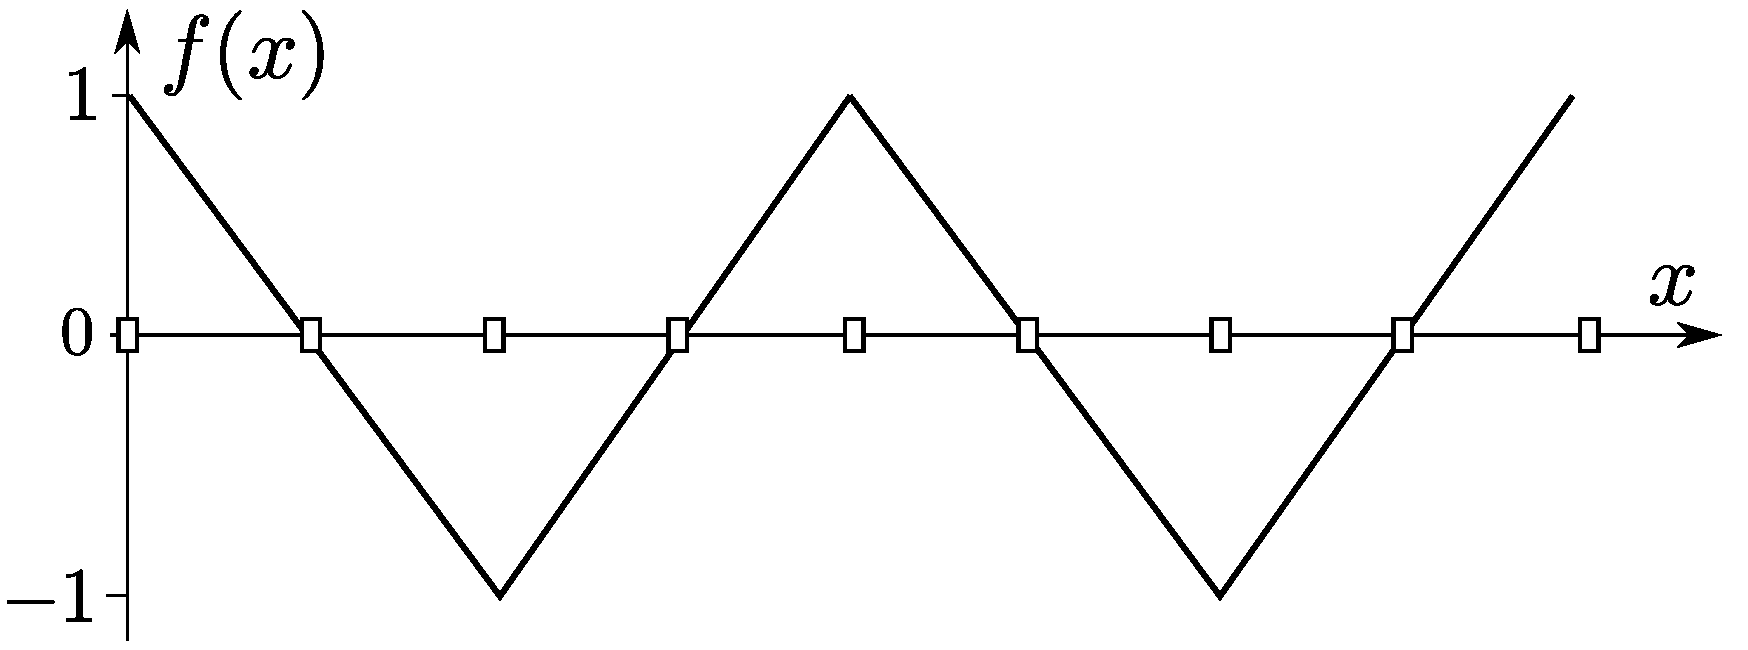
\includegraphics[scale=0.4]
{graphics/invisible_gradient.pdf}%
\caption{An example of invisible function for the gradient operator.}%
\label{parasite}%
\end{figure}
%EndExpansion


This situation arises when the boundary conditions are not considered, but it
can take place also far from the boundaries of a calculation domain. The
bilinear forms resulting from the variational formulations of the
Navier--Stokes equations do not always satisfy the inf--sup condition. A
well-known condition for internal flows of incompressible fluids consists in
choosing different elements to represent pressure and velocity: for example, a
quadratic velocity and a linear pressure.
%In principle, this choice is not
%mandatory for compressible fluids and, by extension, for the Saint-Venant
%equations. However, the choice of different elements for velocity and water
%depth gives more regular results. This is exemplified in Plate 5, where a tide
%is simulated on a quarter-circle beach with a quadratic bottom elevation.
%Advection and all dissipative terms are removed from equations. It is clear
%that in this academic situation spurious oscillations occur with a linear
%discretization, but they disappear if the velocity is treated with a
%quasi-bubble discretization (see \cite{atkinson01}\ for more details).
Another solution, efficient with regular mesh and the finite difference method, is to
have two different and staggered meshes for pressure and velocity. Finally,
for elliptic equations, we can use a discretization of the Laplacian, known as
\textquotedblleft non-compatible\textquotedblright, for which the Laplacian is
not, at the discrete level, equal to the divergence of the gradient.
%The result of this method is detailed in Section \ref{equation d'onde}, where the
%Saint-Venant equations are written in the form of a wave equation.

A more thorough examination of these questions, especially for the
Navier--Stokes equations, can be found in references \cite{ciarlet78} and
\cite{raviart86}, and in the more recent work by Pironneau \cite{pironneau88}
on the methods of finite elements for fluids.

%\subsection{Discretisation of the Navier--Stokes equations in a fixed mesh}


%In TELEMAC-3D a fractional-steps method is used for the time discretisation.
%An important aspect of the algorithm is that the horizontal and vertical velocities are
%not treated the same way. Moreover, there are two definitions of the velocity field
%in the algorithm: the one calculated on the basis of the continuity equation so as to ensure
%mass conservation and the one calculated on the basis of the momentum equation. Later on,
%we refer to them as the conservative velocity and the momentum velocity fields.
%The algorithm then consists of several steps, namely:
%\begin{itemize}
%\item an advection step for the momentum horizontal velocities, using the conservative velocity for the advection;
%\item an advection-diffusion step for the momentum vertical velocity, using the conservative velocity field for the advection and the momentum velocity for the diffusion;
%\item a hydrostatic step, which consists of computing the new depth
%together with the conservative horizontal velocities and then deducing the conservative vertical velocity;
%\item a pressure step for computing the non-hydrostatic pressure and calculating the momentum velocity field;
%\item a final advection-diffusion step for tracers, using the conservative velocity field for the advection.
%\end{itemize}
%
%%Each of these steps will be resolved in detail one after the other. Prior to this,
%%however, discretization in space and building up the mesh have to be specified.
%The sections below describe the hydrostatic step, the pressure step and the tracers advection-diffusion step.
%
%\section{Hydrostatic step}
%
%\subsection{Wave equation}
%\begin{equation}
%  \begin{array}{l}
%    \dfrac{\vec{u}_{2D}^{\textcolor{EdfBlue}{A}}-\vec{u}_{2D}^n}{\delta t}
%    + \left(\left(\vec{u}^{\textcolor{EdfBlue}{A}}-\vec{c}\right)\cdot\Grad\right)\vec{u}_{2D}^{\textcolor{EdfBlue}{A}}=0 \medskip \\
%    \dfrac{w^{\textcolor{EdfOrange}{D}}-w^n}{\delta t}+
%    \left(\left(\vec{u}^{\textcolor{EdfOrange}{D}}-\vec{c}\right)\cdot\Grad\right)w^{\textcolor{EdfOrange}{D}}=
%    -g+\Div(\nu\vec{S}\cdot\vec{e}_z)
%  \end{array}
%\end{equation}
%
%\begin{equation}
%  \begin{array}{l}
%    \dfrac{\eta^{n+1}-\eta^{n}}{\delta t}
%    + \nabla_{2D}\cdot \displaystyle{\int_b^\eta\vec{u}_{2D}^{\textcolor{EdfOrange}{D}}}=0 \medskip \\
%    \dfrac{\vec{u}_{2D}^{\textcolor{EdfOrange}{D}}-\vec{u}_{2D}^{\textcolor{EdfBlue}{A}}}{\delta t}=-g\Grad_{2D}\eta^{n+1}
%    +\Div\left(\nu(\vec{S}\cdot\vec{e}_x+\vec{S}\cdot\vec{e}_y)\right)
%  \end{array}
%\end{equation}
%
%\subsection{Vertical velocities}
%
%%The time-discretisation is done following the sequence below:
%
%%\begin{align}
%%&\frac{\tilde{\vec{U}}_{2D}^{n+1}-\vec{U}_{2D}^{n}}{\Delta t} = - \vec{U}^n\cdot\Grad \vec{U}_{2D}^n + \vec{F}_{2D}^{visc^{n+1}} + \tilde{\vec{F}}_{2D}^{n+1}
%%\notag\\
%%&\frac{\eta^{n+1}-\eta^{n}}{\Delta t} = - \DivD\left(\int_b^\eta\tilde{\vec{U}}_{2D}^ndz\right) + F_b^n
%%\notag\\
%%&\frac{\tilde{W}^{n+1}-W^{n}}{\Delta t} = - \vec{U}^n\cdot\Grad W^n + F_z^{visc^{n+1}} + F_z^{n+1}
%%\notag\\
%%&\Div \left(\frac{1}{\rho}\Grad p_d^{n+1}\right) = \frac{1}{\Delta t}\Div\tilde{\vec{U}}^{n+1}
%%\notag\\
%%&\frac{\vec{U}^{n+1}-\tilde{\vec{U}}^{n+1}}{\Delta t} = - \frac{1}{\rho}\Grad p_d^{n+1}
%%\label{eq:NS_FS_timestepping}
%%\end{align}
%%
%%\commentAL{La convection des vitesses est faite
%%avec les vitesses du pas de temps précédent
%%et la convection des traceurs est faite
%%avec $\Delta z W^*$ afin de conserver la masse de traceur.}
%
%\section{Pressure step}
%\begin{equation}
%  \begin{array}{l}
%    \Lap p_d^{n+1} = \dfrac{\rho}{\delta t}\Div\vec{u}^{\textcolor{EdfOrange}{D}} \medskip \\
%    \dfrac{\vec{u}^{n+1}-\vec{u}^{\textcolor{EdfOrange}{D}}}{\delta t} = -\dfrac{1}{\rho}\Grad p_d^{n+1}
%  \end{array}
%\end{equation}
%
%\section{Tracers advection-diffusion}

\newpage

\chapter{Time discretisation in TELEMAC-3D}\label{Chapter3}
In this chapter, we describe the time-scheme used in TELEMAC-3D in 
a continuous-space framework. The aim is to help the reader understand
what comes in the chapter \ref{Chapter4}, where the space-time discretisation
is described\footnote{It is important to bear in mind that demonstrations 
of conservation can only be done with the full space-time discretisation.}.
In TELEMAC-3D, a fractional-steps method is used for the time discretisation.
An important aspect of the algorithm is that the horizontal and vertical velocities are
not treated in the same way. Moreover, there are two definitions of the velocity field
in the algorithm: the one calculated on the basis of the continuity equation so as to ensure
mass conservation and the one calculated on the basis of the momentum equation. Later on,
we refer to them as the conservative velocity field (denoted by $\vec{u}^C$) and the momentum
velocity field (denoted by $\vec{u}$), respectively. 
We recall that the 2D vector corresponding to the $x$ and $y$
components of a 3D vector is denoted with a $2D$ subscript. 
On the other hand, we denote with an $A$ superscript the fields obtained after an advection step.
%while we denote with a $D$ superscript the fields obtained after an advection-diffusion step.
The algorithm then consists of several steps, which order depends on the
option \texttt{DYNAMIC PRESSURE IN WAVE EQUATION}. 
In TELEMAC-3D, we call wave equation the equation solved to calculate
the new water depth values. It is indeed an equation of wave propagation
since we do not solve the coupled system linking $h^{n+1}$ and $\vec{u}^{Cn+1}$,
but rather write $\vec{u}^{Cn+1}$ as a function of $h^{n+1}$ and introduce
this formula into the equation on $h^{n+1}$. There are two options in TELEMAC-3D:
either the dynamic pressure is calculated after the values of $h^{n+1}$ and
$\vec{u}^{Cn+1}$ are known, or it is calculated once $\vec{u}^{Cn+1}$ has been written 
as a function of $h^{n+1}$ based on an intermediate velocity, which is
thereafter corrected through a projection step, and then only $h^{n+1}$ is
calculated. We list the different steps below, for each value of the key-word.

\section{Dynamic pressure calculated after the wave equation 
resolution}
This corresponds to the option \texttt{DYNAMIC PRESSURE IN WAVE EQUATION=NO}, 
which is the one by default in TELEMAC-3D. The algorithm then consists of 
the following steps:
\begin{enumerate}
\item \textbf{an advection step for the momentum horizontal velocities}, 
using the conservative velocity for the advection:
\begin{equation}
    \dfrac{\vec{u}_{2D}^{A}-\vec{u}_{2D}^n}{\delta t} 
    + \left(\vec{u}^{Cn}\cdot\Grad\right)\vec{u}_{2D}^{*}=0 \medskip \\
\end{equation}
\begin{CommentBlock}{Remarks about the advection term $\left(\vec{u}^{C}\cdot\Grad\right)\vec{u}_{2D}^{*}$:}
\begin{itemize}
\item $\vec{u}^{Cn}$ is used as the advecting velocity because it is 
specifically computed so as to be divergence-free at step 5. 
When using a conservative advection scheme, this makes it possible to ensure mass-conservation 
at machine precision, with any discretisation.
It is a very important feature of TELEMAC-3D, especially for dilution studies where scalar conservation is
of primary importance\footnote{In the studies, the meshes are usually quite coarse,
on the one hand because bathymetric data have a limited accuracy, but also to limit
computational times, so that this is really a key-feature.}.
\item The value of $\vec{u}^{C}$ from the current time-step, $\vec{u}^{Cn}$, is used for the advection of the velocity,
while the value of the next time-step, $\vec{u}^{Cn+1}$, is calculated when solving the wave equation.
However, for the sake of simplicity in the notations, in the next chapter about space-time discretisation
we will not write $\vec{u}^{Cn}$ or $\vec{u}^{Cn+1}$, but only $\vec{u}^{C}$ to have lighter notations.
\item the time-discretisation of the advected field $\vec{u}_{2D}$ is not specified yet, which is accounted for by the $*$ superscript. 
Indeed, in TELEMAC-3D there are various methods for the computation
of the advection term: the methods of characteristics, distributive schemes or finite elements can be used.
The basic forms of distributive schemes -- N, PSI, are explicit, while more complex forms can be semi-implicited
in time. On the other hand, the SUPG scheme is implicit and the characteristics method consists of an exact
time-integration between two time-steps. This is dealt with in the section \ref{equations de transport}.
\end{itemize}
\end{CommentBlock}

\item \textbf{an advection-diffusion step for the momentum vertical velocity}, 
using the conservative velocity field for the advection and the momentum velocity for the diffusion:
\begin{equation}
    \dfrac{\tilde{w}^{aux}-w^n}{\delta t}+
    \left(\vec{u}^{Cn}\cdot\Grad\right)w^{*}=
    -g+ \tilde{F}_z+\Div(\nu_Ew^*\cdot\vec{e}_z)
\end{equation}
\begin{CommentBlock}{Remark:}
In this system, the term $\tilde{F}_z$ contains the buoyancy forces, 
Coriolis force, tidal force, source points inputs and outputs 
(isolated or linked through the culvert fomulation), rain and evaporation. 
If present, these terms are treated explicitly.
\end{CommentBlock}
Then, the diffusion term can be partially or fully implicited using 
a coefficient of implicitation for the diffusion $\theta_d$, 
so that this step reads:
\begin{equation}
    \dfrac{\tilde{w}^{aux}-w^n}{\delta t}+
    \left(\vec{u}^{Cn}\cdot\Grad\right)w^{*}=
    -g+ \tilde{F}_z+\Div\left(\nu_E\theta_{d}\Grad \tilde{w}^{aux} + \nu_E(1-\theta_{d})\Grad w^n\right)
\end{equation}
\begin{CommentBlock}{Remark:}
When applying the Finite Elements space-discretisation to this step,
some diffusion boundary terms appear (friction terms), which may actually be treated
implicitely or explicitely. This is described in the section \ref{etape hydrostatique}.
\end{CommentBlock}

\item \textbf{a hydrostatic step}, which consists in computing the new depth
together with the conservative horizontal velocities:
\begin{equation}\label{eq:hydrostatic_first_system}
  \left\{\begin{array}{l}
    \dfrac{\eta^{n+1}-\eta^{n}}{\delta t} 
    + \nabla_{2D}\cdot \displaystyle{\int_b^\eta\tilde{\vec{u}}_{2D}^{n+1}~dz}=0 \medskip \\
    \dfrac{\tilde{\vec{u}}_{2D}^{n+1}-\vec{u}_{2D}^{A}}{\delta t}=-g\Grad_{2D}\eta^{n+1}
    + \tilde{\vec{F}}_{2D}
    +\BDiv (\nu_E \Grad \vec{u}_{2D}^n)\medskip \\
  \end{array}\right.
\end{equation}

This system corresponds to the lines 1, 2 and 4 of \eqref{eq:NS_FS_expanded}, excluding the advection terms
since they have already been treated in the previous fractional step.
%We defined an intermediate velocity field $\vec{u}^{aux}$ such as:
%\begin{equation}
%  \dfrac{\vec{u}_{2D}^{aux}-\vec{u}_{2D}^{A}}{\delta t}= -g\Grad_{2D}\eta^n
%     + \tilde{\vec{F}}_{2D}
%     +\nu_E \left(\theta_d\Lap \vec{u}_{2D}^{aux}+(1-\theta_d)\Lap \vec{u}_{2D}^{n}\right)
%\end{equation}
The diffusion term was written here in a fully explicit form for the sake of simplicity but
the user actually has the choice to partially implicit it using a coefficient $\theta_d$.
This will be described with more details in the section \ref{momentumvariational}.\\

By replacing $\eta$ by $h + b$ in the second line of \eqref{eq:hydrostatic_first_system}
and partially impliciting the water depth with a 
coefficient $\theta_h$, the term $\Grad_{2D}\eta^{n+1}$ of the second line is actually re-written:
\begin{equation}
\Grad_{2D}(\theta_h\eta^{n+1}+(1-\theta_h)\eta^n) = \Grad_{2D}\left(\theta_h h^{n+1}+(1-\theta_h)h^n+b\right)
\end{equation}
We used the fact that $b$ is considered constant in time here.
The user also has the choice to partially implicit the velocity field during this step, using a coefficient
$\theta_u$ in the first line of the system \eqref{eq:hydrostatic_first_system}.
The system \eqref{eq:hydrostatic_first_system} is then modified and reads:
\begin{equation}\label{eq:hydrostatic_second_system}
  \left\{\begin{array}{l}
    \dfrac{h^{n+1}-h^{n}}{\delta t} 
    + \nabla_{2D}\cdot \displaystyle{\int_b^\eta\left(\theta_u\tilde{\vec{u}}_{2D}^{n+1}+(1-\theta_u)\vec{u}_{2D}^n\right)~dz}=0 \medskip \\
    \dfrac{\tilde{\vec{u}}_{2D}^{n+1}-\vec{u}_{2D}^{A}}{\delta t}=-g \theta_h \Grad_{2D}(h^{n+1}-h^n) -g\Grad_{2D}\eta^n
     + \tilde{\vec{F}}_{2D}
     +\BDiv(\nu_E \Grad \vec{u}_{2D}^n)\medskip \\
  \end{array}\right.
\end{equation}
For the resolution of this system,
the expression of $\tilde{\vec{u}}_{2D}^{n+1}$ given by the second 
line is injected into the first line. This yields a propagation equation on $\eta^{n+1}$.
The system \eqref{eq:hydrostatic_first_system} is then modified and reads:
\begin{equation}
   \left\{\begin{array}{l}
   \begin{array}{ll}
    \dfrac{h^{n+1}-h^{n}}{\delta t}+ \nabla_{2D}\cdot \displaystyle{\int_b^\eta
      -\delta t\theta_ug \theta_h \Grad_{2D}(h^{n+1}-h^n)~dz}= &\medskip \\
     & \hspace{-7cm}-\nabla_{2D}\cdot \displaystyle{\int_b^\eta
      \left[\theta_u\vec{u}_{2D}^{aux}+(1-\theta_u)\vec{u}_{2D}^n\right]~dz} \\
  \end{array}\medskip\\
  \dfrac{\vec{u}_{2D}^{aux}-\vec{u}_{2D}^{A}}{\delta t}= -g\Grad_{2D}\eta^n
     + \tilde{\vec{F}}_{2D}
     +\BDiv\left(\nu_E \theta_d\Grad \vec{u}_{2D}^{aux}+\nu_E(1-\theta_d)\Grad \vec{u}_{2D}^{n}\right)\medskip\\
    \tilde{\vec{u}}_{2D}^{n+1}=\vec{u}_{2D}^{aux}-g \theta_h \delta t\Grad_{2D}(h^{n+1}-h^n)
        \end{array}\right.
\label{eq:wave_equation_time}
\end{equation}
where we display the scheme using $\theta_d$ for partial implicitation of the diffusion.
Solving the first line of this system provides the value of $h^{n+1}$. 
The field $\vec{u}_{2D}^{Cn+1}$ to be used for the advection at the next time-step is then defined by:
\begin{equation}
\vec{u}_{2D}^{Cn+1}=\theta_u\vec{u}_{2D}^{aux}+(1-\theta_u)\vec{u}_{2D}^n
\label{eq:uc}
\end{equation}
so as to be consistent with the conservation of the scalars (see the section
\ref{masse traceur}).
\item \textbf{a step of mesh motion} where the new layers elevations are 
calulcated based on the new values of water depth.
\item \textbf{a pressure step} for computing the dynamic pressure and calculating the momentum velocity field:
\begin{equation}
  \left\{\begin{array}{l}
    \Lap p_d^{n+1} = \dfrac{\rho}{\delta t}\Div \tilde{\vec{u}}^{n+1} \medskip \\
    \dfrac{\vec{u}^{n+1}-\tilde{\vec{u}}^{n+1}}{\delta t} = -\dfrac{1}{\rho}\Grad p_d^{n+1}
  \end{array}\right.
\end{equation}
where $\tilde{\vec{u}}^{n+1}$ is defined by:
%denotes the non divergence-free vector of components $(u^C, v^C, w^C)$.
\begin{equation}
\tilde{\vec{u}}^{n+1}=\vec{u}_{2D}^{aux}-\delta tg\theta_h\Grad_{2D}(h^{n+1}-h^n)+\tilde{w}^{aux}\vec{e}_z
\end{equation}

\begin{CommentBlock}{Remark:}
This step corresponds to the resolution of the Navier--Stokes equations using a Chorin-Temam type 
projection method (see the section \ref{sec:Chorin}) where $\tilde{\vec{u}}^{n+1}$ is the predicted velocity field.
\end{CommentBlock}

\item a step for the \textbf{computation of the conservative vertical velocity}:
\begin{equation}
  \dfrac{\partial w^{Cn+1}}{\partial z}=-\dfrac{\partial u^{Cn+1}}{\partial x}-\dfrac{\partial v^{Cn+1}}{\partial y}, ~w^{C}|_b=0
\end{equation}
\item \textbf{a final advection-diffusion step for scalars} 
(including $k$ and $\epsilon$ when the $k-\epsilon$ turbulence model is used), 
using the conservative velocity field for the advection:
\begin{equation}\label{eq:keps_discreteTime}
  \left\{
    \begin{array}{l}
      \dfrac{k^{n+1}-k^n}{\delta t} +\vec{u}^{Cn+1}\cdot\Grad k^{*}= \mathbb{P}^n + \mathbb{G}^n - \epsilon^n \dfrac{k^{n+1}}{k^n} + \Div(\nu_{k}^n\theta_d\Grad k^{n+1}+\nu_{k}^n(1-\theta_d)\Grad k^{n}) \smallskip \\
      \dfrac{\epsilon^{n+1}-\epsilon^n}{\delta t} +\vec{u}^C\cdot\Grad \epsilon^{*}= \dfrac{\epsilon^n}{k^n}\left(C_{\epsilon_1}\mathbb{P}^n
        +C_{\epsilon_3}\mathbb{G}^n-C_{\epsilon_2,Y}^n\epsilon^{n+1}\right)+\Div(\nu_{\epsilon}^n\theta_d\Grad \epsilon^{n+1}+\nu_{\epsilon}^n(1-\theta_d)\Grad \epsilon^n)
    \end{array}
  \right.
\end{equation}
See the section \ref{sec:kepsequations} for the definitions of $\mathbb{P}$, $\mathbb{G}$, $\mu_{k}$, $\mu_{\epsilon}$, etc. 
$\nu_T^{n+1}$ is then calculated through the equation \eqref{eq:nut} 
and for remaining scalars (temperature, salinity, etc), the following time-discretised equation is solved:
\begin{equation}
  \dfrac{T^{n+1}-T^n}{\delta t}+\vec{u}^{Cn+1}\cdot\Grad T^{*} = F_{source}+\Div(K_T^{n+1}\theta_d\Grad T^{n+1}+K_T^{n+1}(1-\theta_d)\Grad T^n)
\end{equation}

%\textcolor{red}{Termes source explicites / implicites ??} 

\begin{CommentBlock}{Hydrostatic model}
In TELEMAC-3D, it is possible to solve the Navier--Stokes equations with the assumption 
of hydrostatic pressure: the pressure step (step 5) is then entirely skipped.
However, we highly recommend the use the non-hydrostatic option given the poor results
obtained with the hydrostatic option on some cases, in particular when active scalars have a significant
effect on the flow or for wave simulations.
\end{CommentBlock}
\end{enumerate}

\section{Dynamic pressure calculated during the wave equation
resolution}\label{sec:dynamicpressureinwaveequation}
This corresponds to the option \texttt{DYNAMIC PRESSURE IN WAVE EQUATION=YES}.
The algorithm is then modified compared to the one above:
\begin{enumerate}
\item \textbf{the advection step for the momentum horizontal velocities} is unchanged;
\item \textbf{the advection-diffusion step for the momentum vertical velocity}
is also unchanged;
\item \textbf{the hydrostatic step}, is modified. The equations to be solved
now read:
\begin{equation}\label{eq:hydrostatic_third_system}
  \left\{\begin{array}{l}
    \dfrac{h^{n+1}-h^{n}}{\delta t} 
    + \nabla_{2D}\cdot \displaystyle{\int_b^\eta\left(\theta_u\vec{u}_{2D}^{n+1}+(1-\theta_u)\vec{u}_{2D}^n\right)~dz}=0 \medskip \\
    \begin{array}{ll}\dfrac{\vec{u}_{2D}^{n+1}-\vec{u}_{2D}^{n}}{\delta t}&=-g \theta_h \Grad_{2D}(h^{n+1}-h^n) -g\Grad_{2D}\eta^n
     + \tilde{\vec{F}}_{2D}\medskip \\
     &+\BDiv(\nu_E \theta_d\Grad \tilde{\vec{u}}_{2D}^{aux}+\nu_E(1-\theta_d)\Grad \vec{u}_{2D}^{n})
     -\dfrac{1}{\rho}\Grad p_d^n
  \end{array}
\end{array}\right.
\end{equation}
First, a predicted velocity field $\tilde{\vec{u}}^{aux}$ is calculated:
\begin{equation}
  \dfrac{\tilde{\vec{u}}_{2D}^{aux}-\vec{u}_{2D}^{A}}{\delta t}= -g\Grad_{2D}\eta^n
     + \tilde{\vec{F}}_{2D}
     +\BDiv(\nu_E \theta_d\Grad \tilde{\vec{u}}_{2D}^{aux}+\nu_E(1-\theta_d)\Grad \vec{u}_{2D}^{n})
\end{equation}
The projection method is then applied so as to calculate the dynamic pressure 
at this stage and to find a divergence-free velocity field $\vec{u}^{aux}$:
\begin{equation}
  \left\{\begin{array}{l}
    \Lap p_d^{n+1} = \dfrac{\rho}{\delta t}\Div \tilde{\vec{u}}^{aux} \medskip \\
    \dfrac{\vec{u}^{aux}-\tilde{\vec{u}}^{aux}}{\delta t} = -\dfrac{1}{\rho}\Grad p_d^{n+1}
  \end{array}\right.
\end{equation}

The expression of $\vec{u}_{2D}^{aux}$ is then used to replace $\vec{u}_{2D}^{n+1}$
in the first line of \eqref{eq:hydrostatic_third_system}:
\begin{equation}
  \begin{array}{ll}
    \dfrac{h^{n+1}-h^{n}}{\delta t}+ \nabla_{2D}\cdot \displaystyle{\int_b^\eta
      -\delta t\theta_u
            g \theta_h \Grad_{2D}(h^{n+1}-h^n) 
      ~dz}= &\medskip \\

     & \hspace{-7cm}-\nabla_{2D}\cdot \displaystyle{\int_b^\eta
      \left[\theta_u\vec{u}_{2D}^{aux}+(1-\theta_u)\vec{u}_{2D}^n\right]~dz}
  \end{array}
\label{eq:wave_equation_time2}
\end{equation}
Solving this system provides the value of $h^{n+1}$. The value of $\vec{u}_{2D}^{Cn+1}$ is then obtained through:
\begin{equation}
\vec{u}_{2D}^{Cn+1}=\theta_u\vec{u}_{2D}^{aux}+(1-\theta_u)\vec{u}_{2D}^n
\end{equation}
%by solving the second line of \eqref{eq:hydrostatic_second_system}.

\item \textbf{a step of mesh motion}, which is unchanged;

\item a step for the \textbf{computation of the conservative vertical velocity},
which is unchanged;
\item \textbf{a final advection-diffusion step for scalars}, also unchanged.
\end{enumerate}


\newpage

\chapter{Space-time discretisation in TELEMAC-3D}\label{Chapter4}
The chosen spatial discretization is a finite element discretization using
prisms. Each prism has six nodes with quadrangular
vertical sides. The prism with linear interpolation has been retained because its two-dimensional
horizontal projection constitutes one of the finite elements (triangle with
linear interpolation) used to resolve the Saint-Venant equations in two
dimensions. It is thus possible to build a three-dimensional mesh from a
two-dimensional mesh. It only requires to mesh the two-dimensional domain
$\Omega_{2D}$ with triangles, then to duplicate this mesh vertically as
sketched in the figure \ref{maillage 3D 1}.
Calculation in two and three dimensions with the same mesh is thus possible.

In this chapter, we drop the time superscripts in the notation of the
conservative velocity field $\vec{u}^C$ for the sake of simplicity in the notations.
It is always $\vec{u}^{Cn}$ when involved in the advection of the velocity,
and $\vec{u}^{Cn+1}$ everywhere else.

\begin{figure}[tbh]%
\centering
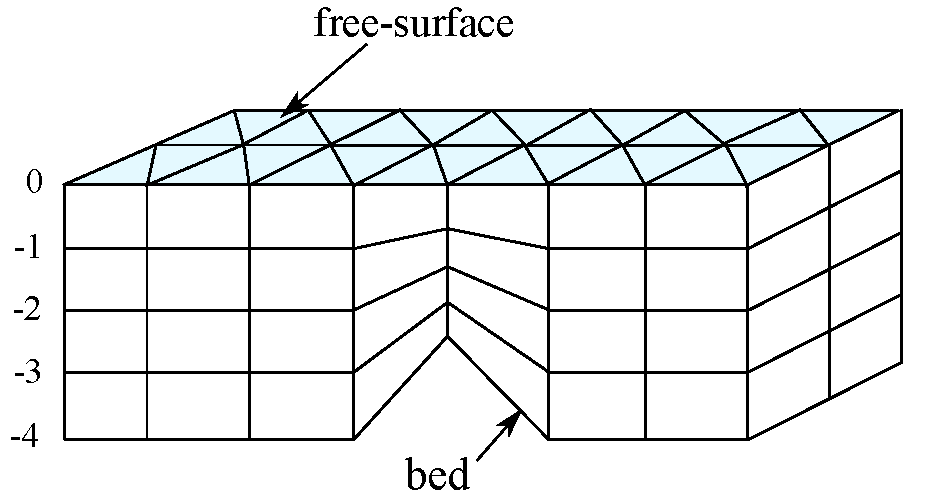
\includegraphics[scale=0.5]{graphics/classical_mesh.pdf}%
\caption{3-D mesh built from a 2-D mesh with a constant proportionality coefficient per plane.}%
\label{maillage 3D 1}%
\end{figure}

\nomenclature[D_z_ip]{$z_{ip}$}{$z$ component of node $i$ in plane $p$ \dotfill (m)}
\nomenclature[D_z*]{$z^*$}{$z$ component in the transformed domain \dotfill (-)}
\nomenclature[D_Delta_z]{$\Delta z$}{Height of a layer in the mesh;
can also be defined as $\partial z/\partial z^*$ \dotfill (m)}
\nomenclature[D_delta_t]{$\delta t$}{Time step \dotfill (s)}

\section{\label{maillage 3D}Building the three-dimensional mesh}

To build the three-dimensional domain with prisms, it is possible to build the
triangulation of the two-dimensional domain, then to repeat it along the
vertical in superimposed layers (called \textquotedblleft
planes\textquotedblright). These \textquotedblleft planes\textquotedblright%
\ are in fact surfaces with variable elevations. The only condition is that
the elevation of the points belonging to a vertical line should increase from the
bed to the free surface. Several simple formulae guarantee this condition,
as in the following four methods.

\subsection{\label{maillage 3D methode 1}Method 1: planes evenly spaced
along the vertical}

This first option, the most classic, consists of starting with the coordinate
nodes $(x,y)$ of the 2D mesh, then defining the elevation for each point of
the 3D mesh with coordinates $(x,y,z)$, according to the formula:%
\begin{equation}
z(x,y,ip)=b\left(  x,y\right)  +\dfrac{ip-1}{np-1}\left(  \eta\left(
x,y\right)  -b\left(  x,y\right)  \right)
\end{equation}
$b$ always being the bed elevation, $\eta$ the free surface elevation
and $ip$ is the rank of the plane under consideration (planes range from $1$
to $np$ if we go from the bed to the free surface). This is the simplest
method based on the sigma transformation (see the section \ref{sec:ALE}.
In this case the vertical coordinate $z^{\ast}$ of each plane in the
transformed mesh is simply $(ip-1)/(np-1)$. The figure \ref{maillage 3D 1}
is a representation of such a mesh.

\subsection{\label{maillage 3D methode 2}Method 2: data of a function
$\theta$ constant for each plane}

The coordinate $z^{\ast}$ of plane $ip$ in the transformed mesh is no longer
$(ip-1)/(np-1)$ but a given number $\theta_{ip}$ such that $0\leq
\theta_{ip}\leq1$ and, for intermediary planes, $\theta_{ip-1}<\theta
_{ip}<\theta_{ip+1}$. We now have:

\begin{equation}
z(x,y,ip)=b\left(  x,y\right)  +\theta_{ip}\left(  \eta\left(
x,y\right)  -b\left(  x,y\right)  \right)
\end{equation}

The figure \ref{maillage 3D 2} shows an example of a 3D mesh built with the
following values:
$\theta_{1}=0,\,\theta_{2}=1/6,\,\theta_{3}=1/3,\,\theta_{4}=2/3,\,\theta_{5}=1$, where the planes are numbered
from the bed to the free-surface. The choice of values of
$\theta_{ip}$ is free, the only constraints being a value of $0$ for the
bed ($ip=1$), a value of 1 for the free surface ($ip=np$) and a series of
intermediate values in a strictly increasing order.

\begin{figure}[tbh]
\centering
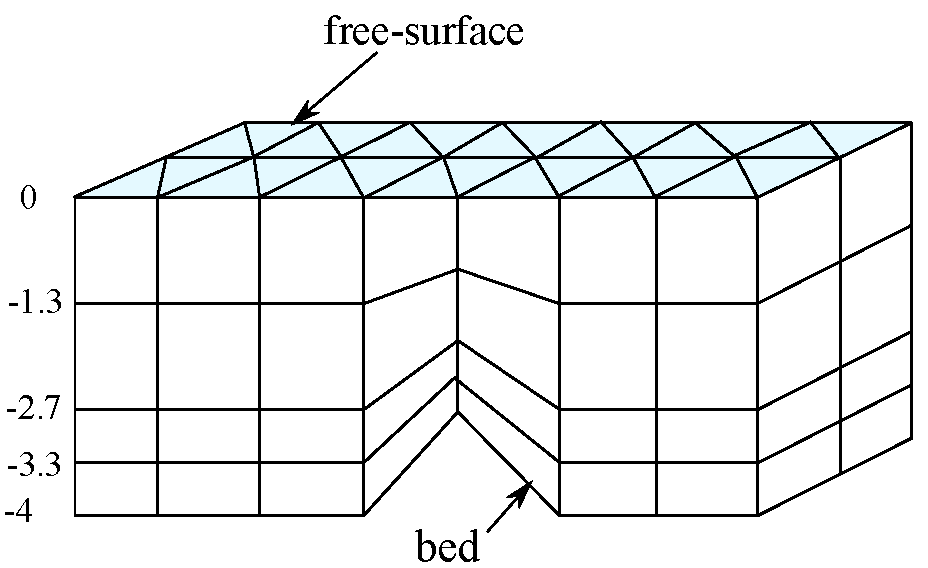
\includegraphics[scale=0.5]{graphics/mesh_theta.pdf}
\caption{Mesh built with a constant proportionality coefficient per plane.}%
\label{maillage 3D 2}
\end{figure}

\subsection{\label{maillage 3D methode 3}Method 3: double sigma transform}

Here we prescribe a constant elevation for one plane, then the planes between
the bed and this plane are evenly spaced, and the same is done between this
plane and the free surface.

\subsection{\label{maillage 3D methode 4}Method 4: horizontal planes}

In order to better represent the temperature stratification zones (thermoclines),
it is sometimes worth imposing a certain number of intermediate
planes to be horizontal. In this case, it is
possible to indicate the desired elevation for each plane, which will be
denoted by $z_{ip}$. This elevation is not always reachable because it can
be located below the bed or above the free surface. In this case, the
elevation of the point of the plane $ip$ will be maintained slightly above the
bed, or slightly below the free-surface. This can be done with the help of a
\textquotedblleft MinMod\textquotedblright\ limiter through the formula:%
\begin{equation}
z=\min\left\{  \max\left[  b(x,y)+\dfrac{ip-1}{np-1}d_{\min},z_{ip}\right]
,\eta(x,y,t)-\dfrac{np-ip}{np-1}d_{\min}\right\}
\end{equation}
where $d_{min}$ is an imposed minimum distance. We impose that plane 1 (the
bed) is at a minimum distance $d_{\min}$ from the free surface, and that
the plane $np$ (the free surface) is at a minimum distance $d_{min}$ from the bed.
The figure \ref{maillage 3D 3} shows an example of a 3D mesh built with this
method and the following prescribed elevations $z_{ip}$: $z_{1}=-4 m,\,z_{2}=-3 m,\,z_{3}%
=-2 m,\,z_{4}=-1 m,\,z_{5}=0 m$.%

\begin{figure}[tbh]%
\centering
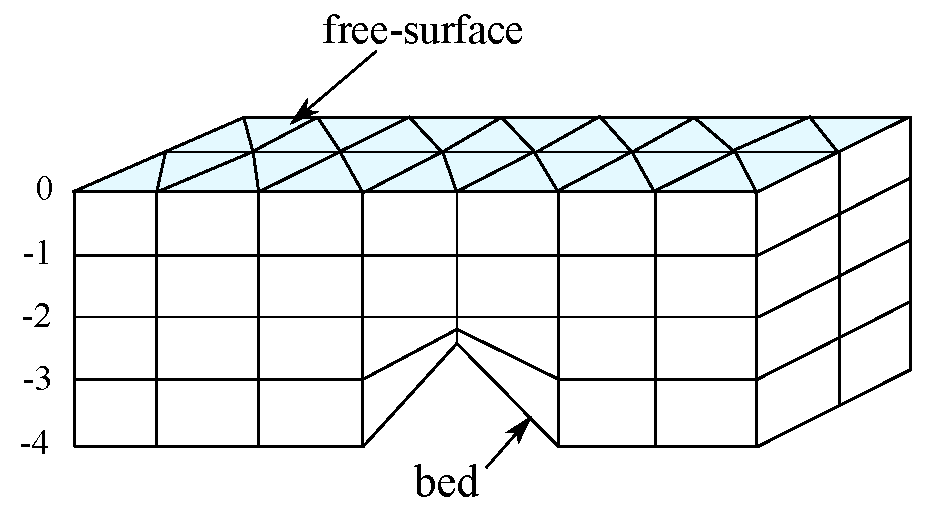
\includegraphics[scale=0.5]{graphics/mesh_horizontal_plane.pdf}
\caption{Example of a 3D mesh with a prescribed horizontal plane at $z=-2m$.}
\label{maillage 3D 3}%
\end{figure}

In conformity with the earlier formula, when the bed rises to the level of
plane number 2 normally situated at elevation $-$3 m, this plane number 2 then
adopts the form of the bed, at a distance $d_{min}/4$.

\begin{CommentBlock}{Comment by J.-M. Hervouet}
The advantage of this distribution is the elimination of truncation errors in
the calculation of buoyancy terms. These errors can generate unacceptable
instability when these terms are dominant. Actually, when the planes are not
horizontal, it is impossible to correctly represent a function $f$ that only
depends on $z$. Now, the density of the fluid should tend to this type of
function corresponding to a position of equilibrium without horizontal
pressure gradients.
With this method, non-horizontal mesh planes are inevitable, but only at a
distance less than $d_{min}$ from the bed or from the surface. In these
zones with quasi-zero volume, it is suggested that the forces arising from the
parasitic horizontal pressure gradients (called hydrostatic inconsistencies)
be cancelled by the intermediary of a filter which acts in places where the
prisms are, such that a node of the lower base (number 1, 2 or 3) has an
elevation higher than a node of the upper base (number 4, 5 or 6). This filter
also cancels the different diffusion coefficients on these elements.
\end{CommentBlock}

\section{\label{transformation sigma}Sigma transformation of the 3D mesh}

As the free surface evolves with time, the elevations $z$ of the 3D mesh vary
from one time step to another. However,
it is possible to change referentials so as to fix the mesh
during a time step. As we have already seen in the section \ref{sec:ALE}, this can
be particularly interesting in the advection step, which has a definite
influence on the evolution of the free surface. The change of variables
adopted in TELEMAC-3D is the sigma transformation, which consists in passing from the
coordinate $z$ to the coordinate $z^{\ast}$, the latter being independent of time.
For the classical sigma transformation, we recall the formula used:%
\begin{equation}
z^{\ast}=\dfrac{z-b}{\eta-b}%
\end{equation}

When a plane has a prescribed constant elevation, a double sigma transform is
preferred, with a function $z^{\ast}$ varying between $-$1 and +1.\ If
$z_{prescribed}$ is the required constant elevation, we have below the fixed plane:
\begin{equation}
z^{\ast}=\dfrac{z-z_{prescribed}}{z_{prescribed}-b}%
\end{equation}
and above:%
\begin{equation}
z^{\ast}=\dfrac{z-z_{prescribed}}{\eta-z_{prescribed}}%
\end{equation}

For a generalized sigma transform, it is convenient to use the following
function $z^{\ast}$ between planes $ip$ and $ip+1$:%
\begin{equation}
z^{\ast}=ip-1+\dfrac{z-z_{ip}}{z_{ip+1}-z_{ip}}%
\end{equation}
where $z_{ip}$ is the elevation of plane $ip$, and$\ z_{ip+1}$ the elevation
of plane $ip+1$. This function $z^{\ast}$ now varies between 0 and $np-1$.
The definition of $z^{\ast}$ is thus univocal over the entire vertical.

\begin{CommentBlock}{Remark:}
These forms of transformation are only necessary when dealing with the full 3D
mesh, \textit{e.g.} during an advection step with the method of characteristics.
For local computations within a single finite element, a local definition is simpler, which reads:
\begin{equation}
z^{\ast}=\dfrac{z-z_{ip}}{z_{ip+1}-z_{ip}}
\end{equation}
\textit{i.e.} we have a classic sigma transformation between two planes.
\end{CommentBlock}

It is interesting to notice that the four methods given above to build the mesh
belong to two different families:
\begin{itemize}
\item the first two are such that $\partial z/\partial z^{\ast}=h$, they thus rely on the classic sigma transformation
\item for the last two, which correspond to generalized sigma transformations:
\begin{equation}
\dfrac{\partial z}{\partial z^{\ast}}=z_{ip+1}-z_{ip}=\Delta z
\end{equation}
\textit{i.e.} the width between two planes, denoted by $\Delta z$. It is only
piecewise constant vertically.
\end{itemize}


\section{\label{equations de transport}Solving transport equations in 3D
\index{advection}%
}

\begin{WarningBlock}{Section under construction}
This section directly comes from the last TELEMAC-3D release notes and has not been
reshaped yet. It contains some explanations regarding the advection schemes but
no general description of the schemes themselves. The notations used in this
section are also the ones from the last release notes.
\end{WarningBlock}

Here we assume that the general problem of advection schemes is known, and we
shall not fully explain the principle of the different techniques. We just
give details on the 3D theory and implementation in specific cases, namely the
method of characteristics, distributive schemes, and the treatment of the
settling velocity.

\subsection{\label{methode des caracteristiques}Method of characteristics%
\index{characteristic curves}%
}

A lot of litterature can be found on the method of characteristics, but in the
case of advection it merely consists in computing pathlines of the flow,
called characteristics (actually trajectories or streamlines if the velocity
is considered constant in time). In the absence of terms other than advection,
the advected variables are constant on the characteristics, and are thus taken
at the previous time step at what is called the foot of the characteristic,
namely the place where was a particule of water that is now on a given point
of the mesh, at the previous time step. \ Basically the method of
characteristics is thus a computation of trajectory followed by an
interpolation. We shall not here describe the navigation in the mesh and how
it works in parallel, but just deal with the specific 3D aspects, the fact
that the advection in TELEMAC-3D is done in a transformed mesh to account for
relocalisation. The theory behind the vertical displacements in the method of
characteristics in 3D is as a matter of fact very tricky and we give hereafter
some explanations. The first thing to understand is that the advection
equation is solved in a transformed mesh with horizontal planes. The sigma
transformation is used to take into account the movement of the mesh.\ As a
matter of fact the physical values at a point in the mesh will change due to
advection terms (velocity of flow) but also due to the movement of the mesh.
It is shown in reference \cite{hervouet007}\ page 21, equation 2.90\ that this can
be simply taken into account by an advection in the transformed mesh. One
would thus expect that the vertical displacements when computing the
characteristics pathlines are of the form:%
\begin{equation}
\Delta z^{\ast}=w^{\ast}\delta t
\end{equation}
using the transformed coordinates and the transformed velocities, but we find
in the implementation the following form:
\begin{equation}
\Delta z^{\ast}=w~\dfrac{ZSTAR(IET+1)-ZSTAR(IET)}{\Delta z}~\delta t
\end{equation}
where $\Delta z$ is the local real width of the given layer between two planes
and $ZSTAR$ is the transformed elevation of planes (here $IET+1$ and $IET$) in
the transformed mesh.

The second thing to understand is then that the velocity $w$ provided by
TELEMAC-3D to the subroutine CHARAC is in fact $w^{\ast}\Delta z$. This
quantity is provided by the subroutine TRIDW2 and has the dimension of a
velocity, it is linked to the real vertical velocity by the formula:%
\begin{equation}
w=\dfrac{\partial z}{\partial t}+u\dfrac{\partial z}{\partial x}+v\dfrac{\partial
z}{\partial y}+w^{\ast}\dfrac{\partial z}{\partial z^{\ast}}%
\end{equation}
where $\partial z/\partial z^{\ast}$ is $\Delta z$ when we apply a
sigma transformation that changes a layer of width $\Delta z$ into a layer of
width 1. Our vertical displacements are thus in reality:%
\begin{equation}
\Delta z^{\ast}=w^{\ast}\dfrac{\partial z}{\partial z^{\ast}}~\dfrac
{ZSTAR(IET+1)-ZSTAR(IET)}{\Delta z}~\delta t
\end{equation}
and $(ZSTAR(IET+1)-ZSTAR(IET))/\Delta z$ is here to give the value
$\partial z^{\ast}/\partial z$ that retrieves the wanted formula
$\Delta z^{\ast}=w^{\ast}\delta t$. At this level we understand that the
values of ZSTAR must correspond to a sigma transformation that changes a layer
$\Delta z$ into a layer of width 1. A solution would be for example that we
have ZSTAR(IET)=IET. This would be simple but this is not exactly what is done.

The third thing to understand:

Actually we are free to apply any correction factor in the vertical
displacements if they are taken into account also in the values of ZSTAR. In
other words we can multiply the coordinates in a layer by any constant without
changing the result. The interest is then that the correction factor
$(ZSTAR(IET+1)-ZSTAR(IET))/\Delta z$ could be a constant independent of
the layer.\ Then the displacements would keep their meaning all over the mesh.
Otherwise we would have to stop at every plane, and recompute a new
displacement compatible with the new metrics (this is done with the
generalised sigma transformation). The denominator being the real width, our
correction factor will be constant if the values of ZSTAR are proportional to
the real z coordinates, for example if they are the values of the array ZSTAR
used for building the mesh, i.e. a sigma transformation giving the whole 3D
mesh a width of 1. For a classical sigma transformation, we have then:%
\begin{equation}
ZSTAR(IET)=\dfrac{IET-1}{NPLAN-1}%
\end{equation}
where NPLAN is the number of planes. The final formula thus mixes two
different sigma transformations, one for computing $w^{\ast}$, one for the
local metrics while navigating in the transformed mesh, and this is not a mistake.

\subsection{\label{schema murd en dimension 3}MURD scheme in three dimensions%
\index{MURD scheme}%
}

The MURD scheme of Janin \cite{janin95}, which signifies \textquotedblleft
Multidimensional Upwind Residual Distribution\textquotedblright, is an
adaptation to prisms of the N and PSI schemes that we have just described for
the triangular meshes. We shall look successively at the two variants: N and PSI.

\subsubsection{N-type MURD scheme}

We work with the transformed fixed mesh and we want to guarantee the global
conservation of the function $f$ by showing that one has:%

\begin{equation}
\int\nolimits_{\Omega^{\ast}}\,\Delta z^{n+1}\dfrac{(f^{n+1}-f^{n})}{\delta t}~
d\Omega^{\ast}+\int\nolimits_{\Omega^{\ast}}\Delta z\vec{u}^{\ast}
\cdot\Grad f^{n}~d\Omega^{\ast}=0
\end{equation}
based on our local equations. We recall that $\vec{u}^{\ast}$ is
made up of the components ($u,v,w^{\ast}$).

The first term is initially written as:%

\begin{equation}
\int\nolimits_{\Omega^{\ast}}\Delta z^{n+1}\dfrac{(f^{n+1}-f^{n})}{\delta
t}~d\Omega^{\ast}=\sum\limits_{ip=1}^{np}\dfrac{(f_{ip}^{n+1}-f_{ip}^{n}%
)}{\delta t}\int\nolimits_{\Omega^{\ast}}\Psi_{ip}^{\ast}\Delta
z^{n+1}~d\Omega^{\ast}
\end{equation}
We later denote:
\begin{equation}
\int\nolimits_{\Omega^{\ast}}\Psi_{ip}^{\ast}\,\Delta z^{n+1}~d\Omega^{\ast
}=S_{ip}%
\end{equation}
to obtain
$\sum\nolimits_{ip=1}^{np}(f_{ip}^{n+1}-f_{ip}^{n})S_{ip}/\delta t$,
the first term of the equation of a point $ip$.
For the second term, $\int\nolimits_{\Omega^{\ast}}\Delta z\vec{u}
\cdot\Grad f^{n}~d\Omega^{\ast}$, we
shall calculate it element by element, and for each element share the
contributions over the points it is made up of. The sum of all our equations
will again give us the global equation desired.

By limiting ourselves to a prism $P^{\ast}$ of the transformed mesh, we shall
thus try to calculate:%

\begin{equation}
\Phi_{P}=\int\nolimits_{P^{\ast}}\Delta z\vec{u}\cdot\Grad(f)~dP^{\ast}
\end{equation}
by trying to put it into the form:
\begin{equation}
\Phi_{P}=\sum\limits_{i=1}^{6}\sum\limits_{j=1}^{6}\lambda_{ij}(f_{i}^{n}-f_{j}^{n})
\end{equation}
with the coefficients $\lambda_{ij}$ positive or zero, as we did for the N
scheme. By decomposing $f$, we already know that:

\begin{equation}
\Phi_{P}=\sum\limits_{i=1}^{6}f_{i}^{n}\int\nolimits_{P^{\ast}}\Delta
z\vec{u}\cdot\Grad\Psi_{i}~dP^{\ast}%
\end{equation}

Now the terms:%
\begin{equation}
\int\nolimits_{P^{\ast}}\Delta z\vec{u}\cdot\Grad\Psi_{i}~dP^{\ast}%
\end{equation}
can be decomposed in horizontal or vertical gradients in the form $a_{i}%
+b_{i}$ with:
\begin{equation}
a_{i}=\int\nolimits_{P^{\ast}}\Delta z u\dfrac{\partial\Psi_{i}}{\partial
x}~dP^{\ast}+\int\nolimits_{P^{\ast}}\Delta z v\dfrac{\partial\Psi_{i}%
}{\partial y}~dP^{\ast}%
\end{equation}
and:%
\begin{equation}
b_{i}=\int\nolimits_{P^{\ast}}\Delta zw^{\ast}\dfrac{\partial\Psi_{i}}{\partial
z^{\ast}}\,dP^{\ast}%
\end{equation}

As we did in Section \ref{wstarmoyen}, we now decompose the bases $\Psi
_{i}(x,y,z^{\ast})$ of the prism into the product $\Psi_{i}^{h}(x,y)\Psi
_{i}^{v}(z^{\ast})$, which gives:%

\begin{equation}
a_{i}=\dfrac{\partial\Psi_{i}^{h}}{\partial x}\int\nolimits_{P^{\ast}}\Delta
z u\Psi_{i}^{v}\,dP^{\ast}+\dfrac{\partial\Psi_{i}^{h}}{\partial y}%
\int\nolimits_{P^{\ast}}\Delta z v\Psi_{i}^{v}\,dP^{\ast}%
\end{equation}
and:%

\begin{equation}
b_{i}=\dfrac{\partial\Psi_{i}^{v}}{\partial z^{\ast}}\int\nolimits_{P^{\ast}%
}\Delta zw^{\ast}\Psi_{i}^{h}\,dP^{\ast}%
\end{equation}

The properties of the bases $\Psi_{i}^{h}(x,y)$ and $\Psi_{i}^{v}(z^{\ast})$
then give us a group of properties for coefficients $a_{i}$ and $b_{i}$:

\begin{itemize}
\item $a_{1}+a_{2}+a_{3}=0$ inferred by $\Psi_{1}^{h}+\Psi_{2}^{h}+\Psi
_{3}^{h}=1$

\item $a_{4}+a_{5}+a_{6}=0$ inferred by $\Psi_{4}^{h}+\Psi_{5}^{h}+\Psi
_{5}^{h}=1$

\item $b_{1}+b_{4}=0$ inferred by $\Psi_{1}^{v}+\Psi_{4}^{v}=1$

\item $b_{2}+b_{5}=0$ inferred by $\Psi_{2}^{v}+\Psi_{5}^{v}=1$

\item $b_{3}+b_{6}=0$ inferred by $\Psi_{3}^{v}+\Psi_{6}^{v}=1$
\end{itemize}

Here, we have again used the local numbering of the points in a prism.

Based on the N scheme, which is built on triangles, a first set of
coefficients $\lambda_{ij}$ could be the following:

\begin{itemize}
\item $\lambda_{ij}=\max(\min(a_{i},-a_{j}),0)$ for the points $i$ and $j$ of
the lower triangle of the prism, or for those of the upper triangle.

\item $\lambda_{i\,i+3}=\max(b_{i},0)$ for the points $i$ of the lower triangle.

\item $\lambda_{i+3\,i}=\max(b_{i+3},0)$ for the points $i$ of the upper triangle.

\item $\lambda_{ij}=0$ for the other terms (which are \textquotedblleft
crossed\textquotedblright\ terms, linking the points which are neither at the
same level, nor on the same vertical line).
\end{itemize}

We already possess all the good properties to construct an N-type scheme (all
the coefficients are positive or zero). However, one could obtain a less
diffusive scheme by transforming the sums of horizontal and vertical fluxes
into crossed fluxes, which can be done by noticing that for a set of three
coefficients $\lambda_{ij}$, $\lambda_{jk}$ and $\lambda_{ik}$, one does not
change the value of $\Phi_{P}$ by carrying out the following series of operations:

\begin{itemize}
\item $\lambda_{ik}=\lambda_{ik}+\min(\lambda_{ij},\lambda_{jk})$

\item $\lambda_{ij}=\lambda_{ij}-\min(\lambda_{ij},\lambda_{jk})$

\item $\lambda_{jk}=\lambda_{jk}-\min(\lambda_{ij},\lambda_{jk})$
\end{itemize}

One in fact observes that the coefficients of $f_{i}^{n}$, $f_{j}^{n}$ and
$f_{k}^{n}$ remain unchanged. We now have a supplementary property, which is
that if a coefficient $\lambda_{ij}$ is strictly positive, then all the
coefficients $\lambda_{jk}$ are zero.

We shall choose, as in two dimensions, the distribution coefficients
$\beta_{i}$ as:%

\begin{equation}
\beta_{i}\Phi_{P}=\sum\limits_{j=1}^{6}\lambda_{ij}(f_{i}^{n}-f_{j}^{n})
\end{equation}
in order to obtain an N-type scheme. Here again, we find a stability criterion
in order to ensure the monotonicity of the scheme:%

\begin{equation}
\delta t\leq\dfrac{S_{i}}{\sum\limits_{\text{neighbouring\thinspace\thinspace
prisms}}\lambda_{ij}}%
\end{equation}


\subsubsection{PSI-type MURD scheme}

Based on our newly found N-type scheme, we need to construct the PSI-type
scheme that will also guarantee that the distribution coefficients fall
between 0 and 1. To do this, in the calculation of $\Phi_{P}$ we need to
separate the positive and negative contributions:%

\begin{equation}
\Phi_{P}=\Phi_{P}^{+}-\Phi_{P}^{-}=\sum\limits_{j=1}^{6}\lambda_{ij}\max
(f_{i}^{n}-f_{j}^{n},0)-\sum\limits_{j=1}^{6}\lambda_{ij}\max(f_{j}^{n}%
-f_{i}^{n},0)
\end{equation}


By comparing $\Phi_{P}^{+}$ and $\Phi_{P}^{-}$, one can modify the scheme N coefficients:

If $\Phi_{P}^{+}\geq\Phi_{P}^{-}$:

\qquad If $f_{j}^{n}\geq f_{i}^{n}$, then $\lambda_{ij}$ is cancelled,

\qquad otherwise $\lambda_{ij}$ is replaced by $\lambda_{ij}\Phi_{P}/\Phi_{P}^{+}$.

If $\Phi_{P}^{+}\leq\Phi_{P}^{-}$:

\qquad If $f_{j}^{n}\geq f_{i}^{n}$, then $\lambda_{ij}$ is replaced by
$-\lambda_{ij}\Phi_{P}/\Phi_{P}^{-}$,

\qquad otherwise $\lambda_{ij}$ is cancelled.

The following is an explanation of these manipulations. In the case where the
positive contributions are the most important, we multiply them by $\Phi_{P}/\Phi_{P}^{+}$
and we cancel the negative contributions. What was $\Phi_{P}^{-}$ is thus cancelled,
what was $\Phi_{P}^{+}$ becomes $\Phi _{P}^{+}\Phi_{P}/\Phi_{P}^{+}=\Phi_{P}$. The final expression for
$\Phi_{P}$ remains unchanged. The case $\Phi_{P}^{+}\leq\Phi_{P}^{-}$ can
easily be deduced.

Following this modification of the coefficients $\lambda_{ij}$, all the terms
$\lambda_{ij}(f_{i}^{n}-f_{j}^{n})$ are positive and all the terms $\beta_{i}$
fall between 0 and 1. Actually:%

\begin{equation}
\beta_{i}=\dfrac{\sum\limits_{j=1}^{6}\lambda_{ij}(f_{i}^{n}-f_{j}^{n})}%
{\Phi_{P}}=\dfrac{\sum\limits_{j=1}^{6}\lambda_{ij}(f_{i}^{n}-f_{j}^{n})}%
{\sum\limits_{l=1}^{6}\sum\limits_{j=1}^{6}\lambda_{ij}(f_{l}^{n}-f_{j}^{n})}%
\end{equation}


All the terms of the summations are positive and the numerator is smaller than
the denominator.

\paragraph{\label{murdconservation}Remarks on mass conservation with the
MURD scheme}

The MURD scheme is perfectly compatible with the proof of scalar mass
conservation set out in Section \ref{masse traceur} and with the continuity
step described in Section \ref{wstarmoyen}. We have in fact said in this
section that:%

\begin{equation}
\Delta zw^{\ast}=\sum\limits_{j=1}^{npoin2}\left[  \Delta zw^{\ast}(z^{\ast
})\right]  _{j}\Psi_{i}^{h}(x,y)
\end{equation}
and $\Delta zw^{\ast}$ is necessary here to calculate the coefficients:%

\begin{equation}
b_{i}=\dfrac{\partial\Psi_{i}^{v}}{\partial z^{\ast}}\int\nolimits_{P^{\ast}%
}\Delta zw^{\ast}\Psi_{i}^{h}\,dP^{\ast}%
\end{equation}


We thus find that:%

\begin{equation}
b_{i}=\sum\limits_{j=1}^{npoin2}\int\nolimits_{\Omega_{2D}}\Psi_{i}^{h}%
\Psi_{j}^{h}\,d\Omega_{2D}\,\,\left\{  \dfrac{\partial\Psi_{i}^{v}}{\partial
z^{\ast}}\int\nolimits_{z_{ip}^{\ast}}^{z_{ip+1}^{\ast}}\left[  \Delta
zw^{\ast}\right]  _{j}\,dz^{\ast}\right\}
\end{equation}


We see that the term in brackets is (ignoring the sign):%

\begin{equation}
\dfrac{1}{(z_{ip}^{\ast}-z_{ip+1}^{\ast})}\int\nolimits_{z_{ip}^{\ast}%
}^{z_{ip+1}^{\ast}}\left[  \Delta zw^{\ast}(z^{\ast})\right]  _{j}~dz^{\ast}%
\end{equation}
which we have denoted $\overline{\left(  \Delta zw^{\ast}\right)}_{ip+1/2}^{j}$.
These terms are produced to resolve the continuity equation.
If mass lumping has been used when computing $\overline{\left(\Delta zw^{\ast}\right)}_{ip+1/2}^{j}$
(see the note at the end of the section \ref{wstarmoyen}), then the coefficients $b_{i}$ must be computed in a
compatible way, which is:%

\begin{equation}
b_{i}=\int\nolimits_{\Omega_{2D}}\Psi_{i}^{h}\,d\Omega_{2D}\,\,\left\{
\dfrac{\partial\Psi_{i}^{v}}{\partial z^{\ast}}\int\nolimits_{z_{ip}^{\ast}%
}^{z_{ip+1}^{\ast}}\left[  \Delta zw^{\ast}\right]  _{i}\,dz^{\ast}\right\}
\end{equation}


%\subsection{A finite volume advection solver}
%
%The main idea is to design an advection solver close to what is done with the
%distributive scheme, i.e. with a splitting of time to ensure the CFL
%condition, with the only modification that the fluxes taken into account are
%not the finite element fluxes, but rather the finite volume point to point
%fluxes which are currently built for the Delwaq interface and for the
%treatment of negative depths in 3D. In 3D and with distributive schemes (full
%explanations on distributive schemes are given in reference \cite{hervouet007}\ from
%page 183 on) we just recall here that we end up in a discretization of
%advection equation in the form:%
%
%\begin{equation}
%S_{i}(\dfrac{C_{i}^{n+1}-C_{i}^{n}}{\delta t})=-\beta_{i}\Phi_{T}%
%\end{equation}
%
%
%Where $S_{i}$ is the integral of the test function of point $i$, $\beta_{i}$
%is a distribution coefficient, $\delta t$ the time step, $C_{i}^{n+1}$the
%value of function $C$ at point $i$ after advection, $C_{i}^{n}$ the value of
%function $C$ at point $i$ before advection. $\Phi_{T}$ actually represents
%$S_{i}(\vec{u}.\Grad(C))$ where $\vec{u}
%$ is the advecting field. The only thing to know here is that $\beta_{i}%
%\Phi_{T}$ is eventually put in the form:%
%
%\begin{equation}
%\beta_{i}\Phi_{T}=\sum\limits_{j}\lambda_{ij}(C_{i}-C_{j})
%\end{equation}
%where the coefficients $\lambda_{ii}$ are zero and all coefficients
%$\lambda_{ij}$ are positive or zero. The sum is done on all the neighbouring
%points of point $i$, i.e. all the points that belong to an element containing
%$i$.
%
%The final value of function $C$ at point $i$ is thus:%
%
%\begin{equation}
%C_{i}^{n+1}=C_{i}^{n}\left(  1-\sum\limits_{j}\lambda_{ij}\dfrac{\delta
%t}{S_{i}}\right)  +\sum\limits_{j}\dfrac{\delta t}{S_{i}}\lambda_{ij}C_{j}^{n}
%\label{finalvalue}%
%\end{equation}
%
%
%Classically, it is said then that the monotonicity criterion consists in
%ensuring that all the coefficients of $f_{i}^{n}$ and $f_{j}^{n}$ be positive,
%which yields, given the fact that all $\lambda_{ij}$ are positive or zero:%
%
%\begin{equation}
%\delta t\leq\dfrac{S_{i}}{\sum\limits_{j}\lambda_{ij}}%
%\end{equation}
%
%
%In finite volumes with fluxes between points, the corresponding equation would be:%
%
%\begin{equation}
%C_{i}^{n+1}=\left(  1-\dfrac{\delta t}{S_{i}}\sum\limits_{j}\max(\Phi
%_{ij},0)\right)  C_{i}^{n}+\sum\limits_{j\text{ }}\dfrac{\delta t}{S_{i}}%
%\max(\Phi_{ij},0)C_{j}^{n}%
%\end{equation}
%
%
%assuming that we start from element by element fluxes in the form:%
%
%\begin{equation}
%\Phi_{i}^{el}=\int\nolimits_{\Omega}\vec{u}.\Grad%
%(\Psi_{i})~d\Omega
%\end{equation}
%
%
%this explains the difference of signs with what was done in 2D where we start
%from fluxes in the form:%
%
%\begin{equation}
%\Phi_{i}^{el}=-\int\nolimits_{\Omega2d}h\vec{u}%
%.\Grad(\Psi_{i})~d(\Omega2d)
%\end{equation}
%
%
%which are fluxes leaving points. This leads us to the following CFL\ condition:%
%
%\begin{equation}
%\delta t\leq\dfrac{S_{i}}{\sum\limits_{j}\max(\Phi_{ij},0)}%
%\end{equation}
%
%
%Implementation should be the same provided that we change everywhere
%$\lambda_{ij}$ by max$(\Phi_{ij},0)$.
%
%In fact, the distributive scheme implementation in subroutine murd3d.f in
%Telemac only uses $\sum\limits_{j}\lambda_{ij}(C_{j}^{n}-C_{i}^{n})$ which is
%array $TRA02$ and $-\sum\limits_{j}\lambda_{ij}$ which is put in array $DB$. A
%finite volume upwind scheme can then be easily implemented if we take:%
%
%\begin{equation}
%DB=-\sum\limits_{j}\max(\Phi_{ij},0)
%\end{equation}
%
%
%and%
%
%\begin{equation}
%TRA02=\sum\limits_{j}\max(\Phi_{ij},0)(C_{j}^{n}-C_{i}^{n})
%\end{equation}
%
%
%Starting from the coefficients $\Phi_{i}^{el}$ (six per element), the point to
%point coefficients $\Phi_{ij}$ are obtained as is done in the interface to
%Delwaq, i.e.:
%
%1) assembling element by element fluxes on points: horizontal fluxes will be a
%sum of two contributions (from the upper and lower layer, except on the bed
%and the free surface).
%
%2) changing the horizontal fluxes of points 1, 2, and 3 in the prism into
%point to point fluxes.\
%
%Points 1 and 2 are done in a subroutine called fluxvfleo\_3d, which calls the
%2D subroutine fluxvfleo.f
%
%3) cancelling all crossed fluxes (between points 1 and 5, 1 and 6, 2 and 4, 2
%and 6, 3 and 4, 3 and 5)
%
%4) finding the vertical fluxes that solve the continuity equation. Comparing
%what is done in subroutine tridw2.f and in subroutine tel4del.f, we find that
%the vertical fluxes are such that:%
%
%\begin{equation}
%\Phi_{ij}=-\Delta z~w^{\ast}%
%%TCIMACRO{\dint \nolimits_{\Omega2d}}%
%%BeginExpansion
%{\displaystyle\int\nolimits_{\Omega2d}}
%%EndExpansion
%\Psi_{k}d(\Omega2d)
%\end{equation}
%
%
%where $\Phi_{ij}$ is the vertical flux between to points $i$ and $j$ located
%in the same prism, on the vertical of the 2D point $k$. On a total of 15
%possible fluxes in the prism, we thus retain 9 non-zero terms, which is
%exactly what is done also with the N-scheme, with the same vertical fluxes.
%Both schemes are actually very close, though different, and it was very easy
%to add the new finite volume scheme as a variant of distributive scheme, in
%subroutine murd3d.f.

\subsection{The case of settling velocity}

We explain here how is done the new advection matrix for the treatment of the
settling velocity $w_{c}$. The treatment described here corresponds to the
keyword ADVECTION-DIFFUSION SCHEME WITH SETTLING VELOCITY = 0, i.e. the
settling velocity is taken into account in a fully implicit way in the
diffusion step. The former treatment consisted of computing first a centered
advection term (call to MATRIX with formula 'MATFGR \ \ \ \ \ \ \ \ \ Z'), and
then upwinding (subroutine upwind, which merely adds a diffusion with a
coefficient $\Delta z~w_{c}/2$, where $\Delta z$\ is the local mesh
size on the vertical). Though this technique would give a perfectly implicit
upwind scheme in a regular one-dimensional mesh, it is more difficult to prove
stability and monotonicity in our 3-dimensional context, with $\Delta z $
depending on the layer and on the position in the underlying 2D mesh.

Our starting equation is in the continuum:%

\begin{equation}
\dfrac{\partial C}{\partial t}+\operatorname{div}(-\vec{w_{c}}C)=0
\end{equation}


As $w_{c}$ is considered positive (version 7.0 on...), we have added the sign
minus to recall that $\vec{w_{c}}$ is a vector pointing downwards.
The equation is solved in the fixed mesh taken at the end of the time step
(since this is also done with diffusion). It is important to start from an
equation written in a conservative form, because $\vec{w_{c}}$ may
be variable in space, and has no reason to be divergence free. Moreover it has
nothing to see with the ambient flow, which would have to be used to simplify
into a non conservative equation.

After discretising the derivative in time and variational formulation, our
equation gives for every point $i$:%

\begin{equation}%
%TCIMACRO{\dint \nolimits_{\Omega}}%
%BeginExpansion
{\displaystyle\int\nolimits_{\Omega}}
%EndExpansion
\Psi_{i}\dfrac{(C^{n+1}-C^{n})}{\delta t}~d\Omega+%
%TCIMACRO{\dint \nolimits_{\Omega}}%
%BeginExpansion
{\displaystyle\int\nolimits_{\Omega}}
%EndExpansion
\Psi_{i}\operatorname{div}(-\vec{w_{c}}C)~d\Omega=0
\end{equation}


Then we integrate by parts the divergence term:%

\begin{equation}%
%TCIMACRO{\dint \nolimits_{\Omega}}%
%BeginExpansion
{\displaystyle\int\nolimits_{\Omega}}
%EndExpansion
\Psi_{i}\dfrac{(C^{n+1}-C^{n})}{\delta t}~d\Omega-%
%TCIMACRO{\dint \nolimits_{\Gamma}}%
%BeginExpansion
{\displaystyle\int\nolimits_{\Gamma}}
%EndExpansion
\Psi_{i}C\vec{w_{c}}~.\vec{n}~d\Gamma+%
%TCIMACRO{\dint \nolimits_{\Omega}}%
%BeginExpansion
{\displaystyle\int\nolimits_{\Omega}}
%EndExpansion
\vec{w_{c}}C\Grad(\Psi_{i}%
)~d\Omega=0
\end{equation}


The boundary term is treated in the boundary conditions, it is on one side the
flux coming from the free surface (i.e. zero) and on the other side the
deposition on the bed. The deposition is discretised with an implicit
concentration, and with mass-lumping, i.e. with the approximation
${\displaystyle\int\nolimits_{\Gamma}}
\Psi_{i}C\vec{w_{c}}~.\vec{n}~d\Gamma\simeq C_{i}^{n+1}%
{\displaystyle\int\nolimits_{\Gamma}}
\Psi_{i}\vec{w_{c}}~.\vec{n}~d\Gamma$. If $w_{c}$ is
constant we see clearly that this term is $-w_{c}C_{i}^{n+1}
{\displaystyle\int\nolimits_{\Omega_{2d}}}
\Psi_{i}~d\Omega_{2d}$. $\Omega_{2d}$ refers to the 2D mesh and is horizontal.
${\displaystyle\int\nolimits_{\Omega_{2d}}}\Psi_{i}~d\Omega_{2d}$
is the area around point $i$ (equivalent to the finite
volume). This term is negative (seen from the suspension it is a loss of
sediment), this is why it is treated implicitly.

Now the matrix corresponding to the term ${\displaystyle\int\nolimits_{\Omega}}
\Psi_{i}\operatorname{div}(-\vec{w_{c}}C)~d\Omega=0$:

This term represents the internal fluxes that change the concentration of a
point (think that ${\int_{\Omega}}\Psi_{i}(C^{n+1}-C^{n})/\delta t~d\Omega$ is the variation of mass).
The matrix will be built element by element, so we restrict to a single prism.
The area associated to points is $SURFAC/3$, where $SURFAC$\ is the area of
the triangle formed by a projection on the horizontal of upper and lower sides
of the prism, or the corresponding triangle in the 2D mesh. Assembling all
$SURFAC/3$ of elements around a point gives ${\displaystyle\int
\nolimits_{\Omega_{2d}}}\Psi_{i}~d\Omega_{2d}$,
the integral of the 2D basis of this point.%

\begin{figure}[h]%
\centering
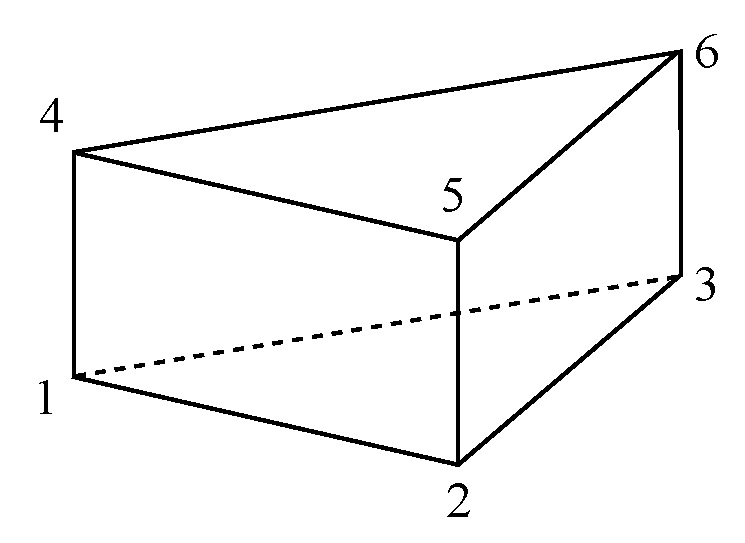
\includegraphics[scale=0.5]{graphics/prism_numbering.pdf}
\caption{Sketch of the prismatic element used in TELEMAC-3D and of the local numbering convention for the nodes.}
\label{schema prisme}%
\end{figure}

To have an upwind treatment of advection we decide that:
\begin{itemize}
\item point 4 looses a flux of $C^{n+1}(4)w_{c}(4)SURFAC/3$
\item point 5 looses a flux of $C^{n+1}(5)w_{c}(5)SURFAC/3$
\item point 6 looses a flux of $C^{n+1}(6)w_{c}(6)SURFAC/3$
\item point 1 receives from point 4 a flux of $C^{n+1}(4)w_{c}(4)SURFAC/3$
\item point 2 receives from point 5 a flux of $C^{n+1}(5)w_{c}(5)SURFAC/3$
\item point 3 receives from point 6 a flux of $C^{n+1}(6)w_{c}(6)SURFAC/3$
\end{itemize}
If we restrict to fluxes into the prism this is all what we see. Of course the
upper points also receive from the upper prism and the lower points give to a
lower prism, but if we restrict here to what we see in the prism there will be
no duplication, and only what receive the points at the free surface and what
give the points at the bed will be forgotten, and it is actually the
boundary terms which are treated elsewhere.

The six fluxes mentionned above result in 6 non zero terms of the element by
element matrix, namely:

$-w_{c}(4)SURFAC/3\qquad$(coefficient of point 4 in equation of point 1, which
is XM(ielem,3))

$-w_{c}(5)SURFAC/3\qquad$(coefficient of point 5 of equation of point 2, which
is XM(ielem,8))

$-w_{c}(6)SURFAC/3\qquad$(coefficient of point 6 of equation of point 3, which
is XM(ielem,12))

$w_{c}(4)SURFAC/3\qquad$(diagonal of 4, which is T(ielem,4))

$w_{c}(5)SURFAC/3\qquad$(diagonal of 5, which is T(ielem,5))

$w_{c}(6)SURFAC/3\qquad$(diagonal of 6, which is T(ielem,6))

This is what is done in subroutine mt15pp.f, then these terms may be assembled
to give the final matrix.

The process of points giving a quantity that is received by others is a proof
of mass-conservation. Note that the diagonals receive positive numbers and the
off-diagonal terms receive negative numbers. The matrix thus built is then a
M-matrix and this ensures the positivity. The matrix will remain always positive-definite.

It would be better to consider that the settling velocities are piece-wise
constant on the vertical, so that we do not consider the settling velocity of
upper points, but an average velocity on the way between upper points and
lower points.

%%%%%%%%%%%%%%%%%%%%%%%%%%%%%%%%%%%%%%%%%%%%%%%%%%%%%%%%%%%%%%%%%%%%%%%%%%%%%%%%%%%%%%%%
%%%%%%%%%%%%%%%%%%%%%%%%%%%%%%%%%%%%%%%%%%%%%%%%%%%%%%%%%%%%%%%%%%%%%%%%%%%%%%%%%%%%%%%%
%%%%%%%%%%%%%%%%%%%%%%%%%%%%%%%%%%%%%%%%%%%%%%%%%%%%%%%%%%%%%%%%%%%%%%%%%%%%%%%%%%%%%%%%
%%%%%%%%%%%%%%%%%%%%%%%%%%%%%%%%%%%%%%%%%%%%%%%%%%%%%%%%%%%%%%%%%%%%%%%%%%%%%%%%%%%%%%%%

\subsection{\label{convection 3D}Other considerations about the advection step}
\index{advection}%

The resolution of the advection equations is described in the chapter
\ref{equations de transport}. This step is executed in the fixed transformed
mesh.
Use of the method of characteristics on the fixed mesh arising from the sigma
transform is not a problem but it may be with other techniques. In order to
show the complications arising from the sigma transform, here is an example of
advection with the SUPG%
\index{SUPG (Streamline Upwind Petrov Galerkin)}
method (described in Chapter \ref{equations de transport}). This method
consists of upwinding the basis functions in the direction of the flow:%

\begin{equation}
\Psi_{i}^{^{\prime}}=\Psi_{i}+\dfrac{\delta t}{2}\vec{u}.\Grad%
(\Psi_{i})
\end{equation}

So, the new basis functions $\Psi_{i}^{^{\prime}}$ remain linear but become
discontinuous. The variational formulation is applied to the following equation:%

\begin{equation}
\dfrac{f^{C}-f^{n}}{\delta t}+\vec{u}^{\ast}.\,\Grad%
^{\ast}\left(  \theta f^{C}+(1-\theta)f^{n}\right)  =0
\end{equation}
where $\theta$ is the relaxation coefficient, $\vec{u}^{\ast}$ the
velocity in the fixed mesh and $\Grad^{\ast}$ the gradient
operator in the same mesh. The earlier equation is multiplied by the deformed
basis function:%

\begin{equation}
\Psi_{i}^{^{\prime}\ast}=\Psi_{i}^{\ast}+\dfrac{\delta t}{2}\vec{u}%
^{\ast}.\Grad(\Psi_{i}^{\ast}) \label{baseupwind}%
\end{equation}
and by using the Einstein notation $f^{C}=f_{j}^{C}\Psi_{j}^{\ast}$, we get:%
\begin{equation}
\dfrac{f_{j}^{C}\Psi_{j}^{\ast}\Psi_{i}^{\prime\ast}}{\delta t}+\theta\Psi
_{i}^{^{\prime}\ast}\vec{u}^{\ast}.\Grad^{\ast
}\left(  f_{j}^{C}\Psi_{j}^{\ast}\right)
\end{equation}

\begin{equation}
=\dfrac{f_{j}^{n}\Psi_{j}^{\ast}\Psi_{i}^{^{\prime}\ast}}{\delta t}+\left(
\theta-1\right)  \;\Psi_{i}^{^{\prime}\ast}\vec{u}^{\ast
}.\Grad^{\ast}\left(  f_{j}^{n}\Psi_{j}^{\ast}\right)
\end{equation}

Strictly speaking, the deformed basis function should be used for all the
terms in the equation. In practice, only the advection term is transformed,
which does not alter the conservation property. After dividing by $\theta$, we get:%

\begin{equation}
f_{j}^{C}\left(  \dfrac{\Psi_{j}^{\ast}\Psi_{i}^{\ast}}{\theta\delta t}%
+\Psi_{i}^{\ast}\vec{u}^{\ast}.\,\Grad^{\ast
}\left(  \Psi_{j}^{\ast}\right)  \right)
\end{equation}
%

\begin{equation}
+f_{j}^{C}\left(  \dfrac{\delta t}{2}\vec{u}^{\ast}.\,\Grad%
^{\ast}\left(  \Psi_{i}^{\ast}\right)  \vec{u}^{\ast}%
.\,\Grad^{\ast}\left(  \Psi_{j}^{\ast}\right)  \right)
=f_{j}^{n}\left(  \dfrac{\Psi_{j}^{\ast}\Psi_{i}^{\ast}}{\theta\delta
t}\right)
\end{equation}
%

\begin{equation}
+f_{j}^{n}\left(  \dfrac{\theta-1}{\theta}\left(  \Psi_{i}^{\ast}%
\vec{u}^{\ast}.\,\Grad^{\ast}\left(  \Psi_{j}%
^{\ast}\right)  +\dfrac{\delta t}{2}\vec{u}^{\ast}.\,\Grad%
^{\ast}\left(  \Psi_{i}^{\ast}\right)  \vec{u}^{\ast}%
.\,\Grad^{\ast}\left(  \Psi_{j}^{\ast}\right)  \right)
\right)
\end{equation}

By multiplying by $h$ and by integrating on the total fixed domain we finally get:%

\begin{equation}
f_{j}^{C}\left(  \dfrac{m_{ij}}{\theta\delta t}+\;vgr_{ij}+ugug_{ij}\right)
=f_{j}^{n}\left(  \dfrac{m_{ij}}{\theta\delta t}+\;\dfrac{\theta-1}{\theta
}\left(  vgr_{ij}+ugug_{ij}\right)  \right)
\end{equation}
with:%

\begin{equation}
m_{ij}=
{\displaystyle\int\nolimits_{\Omega^{\ast}}}
h\Psi_{i}^{\ast}\Psi_{j}^{\ast}~d\Omega^{\ast}=%
{\displaystyle\int\nolimits_{\Omega}}
\Psi_{i}\Psi_{j\,}~d\Omega
\end{equation}

$M$, whose general term is $m_{ij}$, is the mass matrix. It may be estimated
either in the real mesh or in the fixed mesh.%

\begin{equation}
vgr_{ij}=%
{\displaystyle\int\nolimits_{\Omega^{\ast}}}
h\varphi_{i}^{\ast}\vec{u}^{\ast}\cdot\,\Grad^{\ast}\left(
\varphi_{j}^{\ast}\right)  ~d\Omega^{\ast}%
\end{equation}


$VGR$, whose general term is $vgr_{ij}$, is the matrix obtained for classic
advection by finite elements expressed in fixed mesh.%

\begin{equation}
ugug_{ij}=\dfrac{\delta t}{2}%
{\displaystyle\int\nolimits_{\Omega^{\ast}}}
h\vec{u}^{\ast}.\,\Grad^{\ast}\left(  \Psi_{i}^{\ast}\right)
\,\vec{u}^{\ast}.\,\Grad^{\ast}\left(  \Psi
_{j}^{\ast}\right)  ~d\Omega^{\ast}%
\end{equation}

$UGUG$, whose general term is $ugug_{ij}$, is the additional matrix from SUPG.
We show \cite{moulin93} that $ugug_{ij}$ is equivalent to an artificial
diffusion which, in a dimension greater than one, is only produced in the
direction of the current. In 2D, the calculation of the earlier matrices is
relatively short for triangular elements. For prisms with a triangular base,
the number of operations necessary to form the matrices then clearly
increases. In order to simplify the calculation of their coefficients and
observing that, in theory, it does not harm the conservation property, we can
limit $\vec{u}^{\ast}$ in formula \ref{baseupwind}\ to the horizontal
components of velocity. In the case of essentially horizontal flow, this
approximation is not a problem. Only the generic coefficient of the $UGUG$
matrix is modified in this way. It becomes:
\begin{equation}
ugug_{ij}=\dfrac{\delta t}{2}%
{\displaystyle\int\nolimits_{\Omega^{\ast}}}
h\vec{u}_{h}^{\ast}.\,\Grad^{\ast}\left(  \Psi
_{i}^{\ast}\right)  \,\vec{u}^{\ast}.\,\Grad^{\ast
}\left(  \Psi_{j}^{\ast}\right)  ~d\Omega^{\ast}%
\end{equation}
with $\vec{u}_{h}^{\ast}=(u,v,0)$. When this approximation is made
the matrix $UGUG$ is no longer symmetric.

When advection of a variable is done with the help of this method, the steps
of advection and diffusion are in fact treated at the same time.

\section{\label{diffusion 3D}Space discretisation of the diffusion step}

Depending on the chosen advection scheme, the diffusion and advection
are either treated implicitly at the same time (SUPG scheme) or successively,
first calculating the advection (with the characteristics method or a
distributive scheme) and then adding the diffusion to the advected
field. In this section we only consider the discretisation of the
diffusion term. In this section, we denote with a $D$ superscript
the fields obtained after the diffusion has been calculated.
Remember from the chapter \ref{Chapter3} that the diffusion is
hardly ever calculated on its own: it can only be the case for the
vertical velocity prediction, when the advection and diffusion are treated
separately. \\

For the conditions of existence and uniqueness of the solution for the diffusion
problem, which is parabolic, the reader can refer to Raviart and Thomas
\cite{raviart83} or to the book by Pironneau \cite{pironneau88} (in French).\\

Given the complexity of a diffusion stage with the sigma transform, and the
numerical artefacts which are its consequence, this stage is executed in the
real mesh.
The variational formulation of the diffusion step reads:
\begin{equation}
\begin{array}{ll}
\displaystyle{\int_\Omega}\vec{u}^D\cdot\vec{\Psi}_i~d\Omega -
\delta t \theta_d\displaystyle{\int_\Omega}\Div(\nu_{E}\Grad\vec{u}^D)\cdot\vec{\Psi}_i
~d\Omega & = \displaystyle{\int_\Omega}\vec{u}^A\cdot\vec{\Psi}_i~d\Omega \bigskip \\
& +\delta t (1-\theta_d)\displaystyle{\int_\Omega}
\Div(\nu_{E}\Grad\vec{u}^A)\cdot\vec{\Psi}_i~d\Omega
\end{array}\label{eq:diffcont}
\end{equation}
where $\theta_d$ is the coefficient of implicitation of the diffusion.
The vectorial bases $\vec{\Psi}_i$ correspond to a P1 basis on the prism
for each space direction.
In the left-hand side, the second term is written as:
\begin{equation}
\begin{array}{ll}
\displaystyle{\int_\Omega}\Div(\nu_{E}\Grad\vec{u}^D)\cdot\vec{\Psi}_i~d\Omega& =
\displaystyle{\int_\Omega}\Div(\nu_{E}\Grad\vec{u}^D\cdot\vec{\Psi}_i)~d\Omega
-\displaystyle{\int_\Omega}\nu_{E}\Grad\vec{\Psi}_i:\Grad\vec{u}^D~d\Omega \bigskip\\
& =\displaystyle{\int_\Gamma}\nu_{E}\Grad\vec{u}^D\cdot\vec{\Psi}_i\cdot\vec{n}
~d\Gamma - \displaystyle{\int_\Omega}\nu_{E}\Grad\vec{\Psi}_i:\Grad\vec{u}^D~d\Omega\end{array}
\end{equation}
The second line is obtained using the Gauss theorem on the integral of
the divergence. The corresponding boundary integral corresponds to the
friction on the boundaries, which is prescribed.
The Finite Element discretisation of the term $\Grad\vec{u}^D$ reads:
\begin{equation}
\Grad\vec{u}^D=\sum_j \vec{u}_j^D\Grad\vec{\Psi}_j
\end{equation}
The Finite Element discretisation of the equation \eqref{eq:diffcont} then reads:
\begin{equation}
\begin{array}{ll}
\vec{u}_j^D\displaystyle{\int_\Omega}\vec{\Psi}_i\cdot\vec{\Psi}_j~d\Omega +
\delta t \theta_d\nu_{Ej}\vec{u}_j^D\displaystyle{\int_\Omega}\Grad\vec{\Psi}_i
:\Grad\vec{\Psi}_j~d\Omega - \vec{u}_j^D\displaystyle{\int_\Gamma}\nu_{E}\Grad\vec{\Psi}_j
\cdot\vec{\Psi}_i\cdot\vec{n}~d\Gamma& = \vec{u}_j^A\displaystyle{\int_\Omega}
\vec{\Psi}_i\cdot\vec{\Psi}_j~d\Omega \bigskip \\
& ~\hspace{-4cm}+\delta t (1-\theta_d)\nu_{Ej}\vec{u}_j^A\displaystyle{\int_\Omega}
\Grad\vec{\Psi}_i:\Grad\vec{\Psi}_j~d\Omega
\end{array}\label{eq:diff}
\end{equation}
for all degrees of freedom $i$, $j$.
The construction of the diffusion matrix in the real mesh composed of prisms
of arbitrary shape is not easy because the Jacobian of the isoparametric
transformation between an arbitrary prism and the reference prism appears
in the denominator in the calculation of the diffusion matrix.
Indeed, the matrix terms corresponding to the second integral in the
left-hand side are calculated in the reference element:
\begin{equation}
\displaystyle{\int_\Omega}\Grad\vec{\Psi}_i:\Grad\vec{\Psi}_j~d\Omega=
\displaystyle{\int_{\hat{\Omega}}}\Grad\vec{\Psi}_i:\Grad\vec{\Psi}_j
|\vec{J}|~d\hat{\Omega}
\end{equation}
where $\hat{\Omega}$ is the transformation of $\Omega$ into a set of
reference prisms through $F$, defined by \eqref{eq:transfF}
and $|\vec{J}|$ is the Jacobian of $F$, defined by \eqref{eq:jacobian}.
The terms $\Grad\vec{\Psi}_i$ are then written (for example for the first
coefficient of the matrix):
\begin{equation}
(\Grad\vec{\Psi}_i)_{xx}=\dfrac{\partial \Psi_{xi}}{\partial \alpha}\dfrac{\partial \alpha}{\partial x}
\end{equation}
and the term $\partial \alpha / \partial x$ is equal to $1/|\vec{J}|$.
However, this Jacobian is not a constant, therefore
we cannot get a polynomial expression for the matrix coefficients and
their integration over $\hat{\Omega}$ is tricky.
It is however possible to find an approximation of the diffusion matrix on
prisms, \textit{e.g.} by considering a constant average Jacobian on
every prism to get a polynomial expression of the coefficients.
This is what is done at the moment in TELEMAC-3D. \\

This problem does not exist with tetrahedra and a linear interpolation,
the Jacobian then being a constant.
Now, a prism can be broken down into three tetrahedra (see the figure
\ref{decoupage prisme}, where the tetrahedra are formed by the sets of four
points (3,1,2,6), (4,6,5,1) and (5,2,1,6)). Then, let us consider that the
interpolation on the prism is linear by pieces, exactly as in a quasi-bubble
triangle.
As no degree of freedom is added, the topology of a prismatic element matrix
can be formally retained. After calculating the element matrices on the
tetrahedra, a pre-assembly restores the element matrices prism by prism.
Writing this pre-assembly shows that all the properties of a diffusion matrix
(sum of the terms of each line equal to zero, sum of the terms of each column
equal to zero) are actually transferred from the tetrahedra to the prisms.
This technique has been implemented in TELEMAC-3D but is not used at the moment.
The advantage of this technique compared to the
approximate diffusion matrix on prisms is not obvious in
preliminary numerical tests.
\begin{figure}[tbh]%
\centering
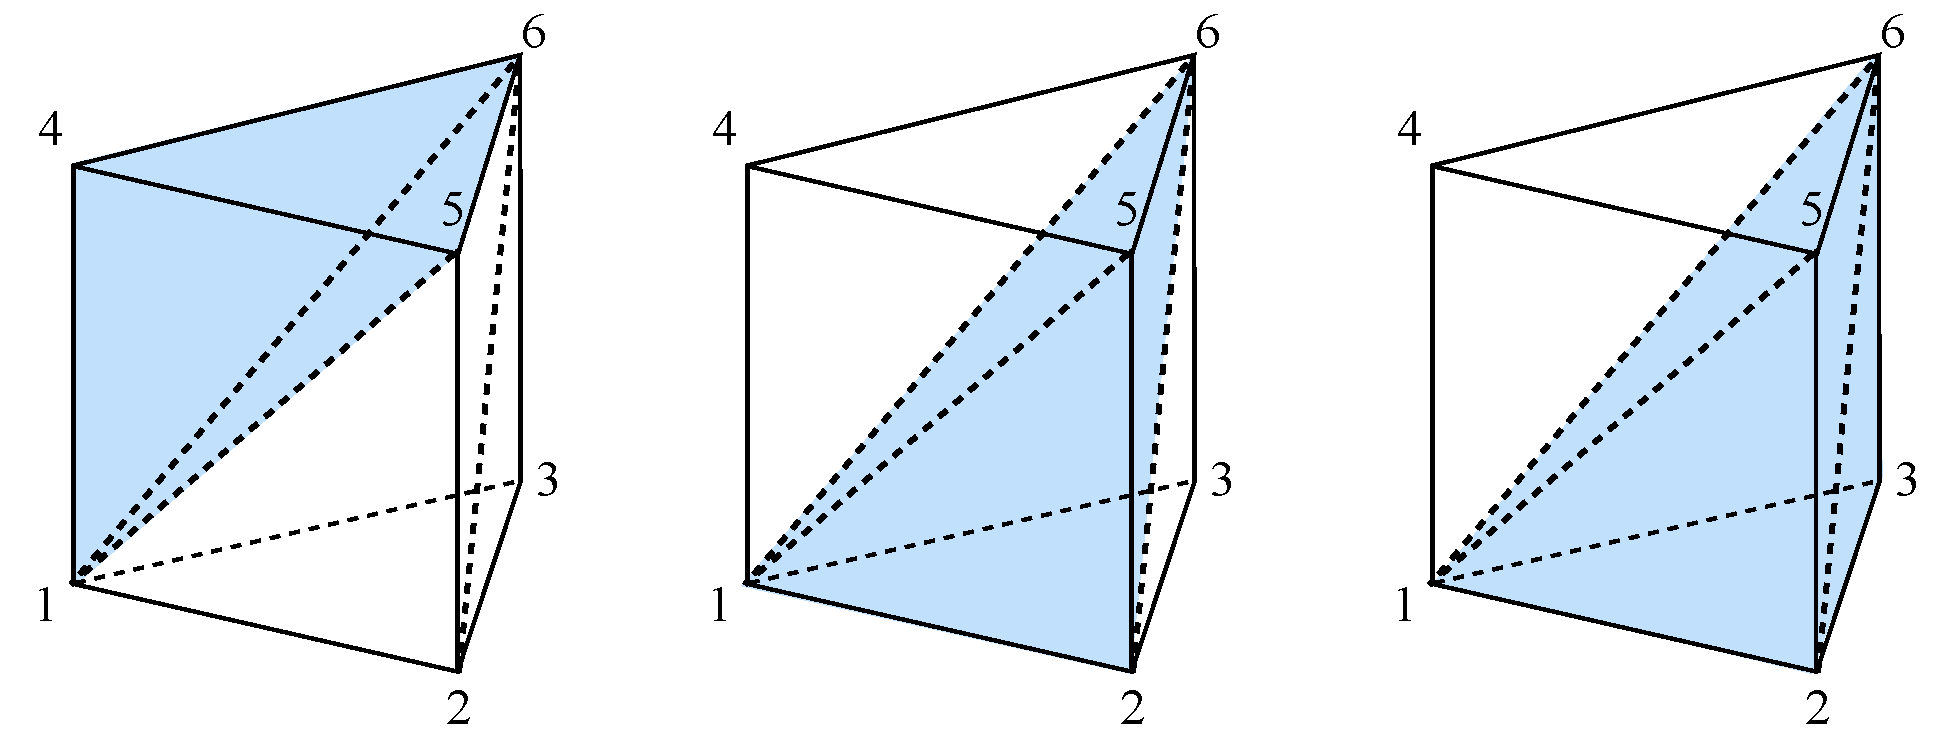
\includegraphics[scale=0.4]{graphics/prism_tetra.pdf}%
\caption{Decomposition of a prism into three tetrahedra.}%
\label{decoupage prisme}%
\end{figure}


\begin{CommentBlock}{Important remark:}
The diffusion matrix should only possess negative extra-diagonal terms
and the sum of each line should always yield zero in order
to achieve monotonicity and conservation.
However, from the computational point of view the extra-diagonal terms
can happen to be positive. Thus, the diffusion matrix in TELEMAC-3D
is modified: all extra-diagonal terms are clipped to a maximum value
of zero and the diagonal terms are modified so as to always retrieve
a zero-sum of each line. %Thus, monotonicity and conservation are ensured.
\end{CommentBlock}

With distributive schemes or when the user chooses to explicit the
diffusion ($\theta_d=0$), the first term in the left-hand side is mass-lumped
and \eqref{eq:diff} reads:
\begin{equation}
\begin{array}{ll}
\vec{u}_j^D\displaystyle{\int_\Omega}\vec{\Psi}_i~d\Omega +
\delta t \theta_d\nu_{Ej}\vec{u}_j^D\displaystyle{\int_\Omega}\Grad\vec{\Psi}_i
:\Grad\vec{\Psi}_j~d\Omega & = \vec{u}_j^A\displaystyle{\int_\Omega}
\vec{\Psi}_i\vec{\Psi}_j~d\Omega \bigskip \\
& ~\hspace{-4cm}+\delta t (1-\theta_d)\vec{u}_j^A\displaystyle{\int_\Omega}
\vec{\Psi}_i\Div(\nu_{Ej}\Grad\vec{\Psi}_j)~d\Omega
+\displaystyle{\int_\Gamma}\nu_{E}\Grad\vec{u}^D\cdot\vec{\Psi}_i\cdot\vec{n}
~d\Gamma
\end{array}
\end{equation}

\begin{CommentBlock}{Mass-lumping:}
The mass-lumping corresponds to a modification of a matrix
to obtain a diagonal matrix where all the extra-diagonal components
were summed onto the diagonal, line by line. This constitutes
an approximation of the original matrix but simplifies the
resolution of the system since only a division by the diagonal is
necessary.
\end{CommentBlock}

\begin{CommentBlock}{Remark:}
The calculation of $\displaystyle{\int_\Omega}\vec{\Psi}_i~d\Omega$ in the
left-hand side is done in agreement with the choice of mass-lumping for
the water heigth term in the wave equation (see the section
\ref{sec:masslumping}).
\end{CommentBlock}

\subsection{\label{calcul flottabilite 3D}Buoyancy terms%
\index{buoyancy}%
}

The source terms of buoyancy are one of the strategic points of 3D equations.
Their correct treatment conditions the representation of stratifications, a
current stumbling block of modelling. These source terms are, if we do not
consider atmospheric pressure (see the section \ref{sec:boussinesq}):%

\begin{equation}
F_{x}=g\dfrac{\Delta\rho}{\rho_{o}}\left(  \dfrac{\partial \eta}{\partial
x}\right)  _{y,t}-g\dfrac{\partial}{\partial x}\left(  \int\nolimits_{z}%
^{\eta}\dfrac{\Delta\rho}{\rho_{o}}\,dz\right)  _{y,z,t}%
\end{equation}
%
\begin{equation}
F_{y}=g\dfrac{\Delta\rho}{\rho_{o}}\left(  \dfrac{\partial \eta}{\partial
y}\right)  _{x,t}-g\dfrac{\partial}{\partial y}\left(  \int\nolimits_{z}%
^{\eta}\dfrac{\Delta\rho}{\rho_{o}}\,dz\right)  _{x,z,t}%
\end{equation}
%
The terms $F_{x}$ and $F_{y}$ are calculated on the mesh at time $t^{n}$ on
the basis of differences in density $\Delta\rho$. These differences in density
themselves have been evaluated earlier with the help of a state function in
which the different concentrations of active scalars appear.
Bijvelds \cite{bijvelds01} compares the treatment of these terms in sigma
transform formulation, in different software.
The term $F_{x}$ can be calculated either in the real mesh or in the transformed mesh.
In TELEMAC-3D, the calculation is done in the real mesh.
%Given below are two modes of
%calculation, limited to the term $F_{x}$, the first in the real mesh and the
%second in the transformed mesh.

\paragraph{Calculation in the real mesh:}

the second term of $F_{x}$\ cannot be directly expressed in the form of
vectors in finite elements. It has to be transformed with the Leibnitz formula
to obtain:%

\begin{equation}
-g\dfrac{\partial}{\partial x}\left(  \int\nolimits_{z}^{\eta}\dfrac{\Delta
\rho}{\rho_{o}}\,dz\right)  _{y,z,t}=-g\left[  \int\nolimits_{z}^{\eta}%
\dfrac{\partial}{\partial x}\left(  \dfrac{\Delta\rho}{\rho_{o}}\right)
\,dz+\dfrac{\Delta\rho(\eta)}{\rho_{o}}\dfrac{\partial \eta}{\partial x}\right]
\end{equation}


We finally get:%

\begin{equation}
F_{x}=-g\int\nolimits_{z}^{\eta}\dfrac{\partial}{\partial x}\left(
\dfrac{\Delta\rho}{\rho_{o}}\right)  \,dz+g\dfrac{\partial \eta}{\partial
x}\left(  \dfrac{\Delta\rho(z)}{\rho_{o}}-\dfrac{\Delta\rho(\eta)}{\rho_{o}%
}\right)
\end{equation}


This formula is simply calculated by using vertical lines of the mesh for the
integral along $z$ and to find the value of $\Delta\rho(\eta)$ above one point
of elevation $z$.

\begin{CommentBlock}{Remark:}
The Appendix B \ref{appendixB}
explains how these terms can be calculated in
the transformed mesh. TELEMAC-3D contains the corresponding code but it is not
used at the moment.
\end{CommentBlock}

\subsection{\label{friction3D}Friction terms%
\index{friction}%
}
Compatibility between friction terms in 2D and 3D is discussed in
\cite{hervouet007}; however, this is only valid for formulae relying on a
depth-integrated velocity, such as those of Strickler%
\index{Strickler!formula}
or Ch\'{e}zy%
\index{Ch\'{e}zy!formula}%
. If we want to use a local roughness factor and assume a logarithmic profile
near the bed, the friction velocity $u_{\ast}$ has to be evaluated. We can
use the fact that the mesh of prisms is made of piled-up meshes of triangles
and consider the first plane above the bed. If we assume that this first
plane is still in the logarithmic profile, we can write (the example of a
hydraulically rough flow):%
\index{rough flow}%
%
\begin{equation}
u_*=\dfrac{\kappa u_{plane\,1}}{\ln\left(\dfrac{33\Delta z}{k_{s}}\right)}%
\end{equation}
where $u_{plane\,1}$ is the velocity at the first point above the bed and
$\Delta z$ the altitude of this point above the bed.

\subsection{\label{calcul termes sources 3D}Other source terms}

The other source terms included in the terms $F_{x}$ and $F_{y}$\ are also
treated in the diffusion stage, explicitly (Coriolis, source points, culverts,
rain and evaporation, tidal forcing, etc.).

\section{\label{etape hydrostatique}Space discretisation of the hydrostatic step}
Here we only consider the case where the dynamic pressure is calculated after the resolution of
the hydrostatic step. We recall that we wrote the following system for the calculation of $h^{n+1}-h^{n}$ and
$\tilde{\vec{u}}_{2D}^{n+1}$ in the section \ref{Chapter3}:
\begin{equation}
  \left\{\begin{array}{l}
    \dfrac{h^{n+1}-h^{n}}{\delta t}
    + \nabla_{2D}\cdot \displaystyle{\int_b^\eta\left(\theta_u\tilde{\vec{u}}_{2D}^{n+1}+(1-\theta_u)\vec{u}_{2D}^n\right)~dz}=0 \medskip \\
    \dfrac{\tilde{\vec{u}}_{2D}^{n+1}-\vec{u}_{2D}^{A}}{\delta t}=-g \theta_h \Grad_{2D}(h^{n+1}-h^n) -g\Grad_{2D}\eta^n
     + \tilde{\vec{F}}_{2D}
     +\Div(\nu_E \Grad \vec{u}_{2D}) \medskip \\
  \end{array}\right.
\label{eq:systeme_hydrostatique}
\end{equation}
The time-discretisation for the diffusion term in the second line will be specified later.
In the sub-sections \ref{continuitytransformed} and \ref{momentumvariational},
a variational formulation for the depth-integrated
continuity equation (first line of this system) and for the horizontal momentum equation (second line)
are derived. The latter will provide an expression of $\tilde{\vec{u}}_{2D}^{n+1}$,
that is introduced in the first line in order to calculate $h^{n+1}$.
Once $h^{n+1}$ is known, the value of $\tilde{\vec{u}}_{2D}^{n+1}$ is retrieved through the horizontal
momentum equation. In between, a conservative velocity $\vec{u}_{2D}^C$ will have been calculated,
which is the one used for the advection terms.

%In the momentum equation, increments of the water depth are made to appear by
%a semi-implicitation of the free surface, like for the Saint-Venant equations:%
%
%\begin{equation}
%\begin{array}{l}
%\dfrac{\vec{u}^{C}-\vec{u}^{A}}{\delta t}= \\
%-s1u\,\,\vec{u}^{n+1}-g\theta_{h}\,\Grad%
%(h^{n+1}-h^{n})-g\,\Grad(\eta^{n})-\dfrac{1}{\rho
%}\Grad(p_{d})+\vec{F}+div(\nu_{t}%
%\Grad(\vec{u}))
%\end{array}
%\end{equation}
%\begin{WarningBlock}{Dynamic pressure + s1u source terms}
%The gradient of an estimated dynamic pressure can be included in the momentum equation at this stage.
%Describe it? It is an option right?
%Also, what to do with the s1u notation?
%\end{WarningBlock}


\subsection{\label{continuitytransformed}Variational formulation of the depth-integrated continuity equation in the transformed mesh}

The time-space discretised depth-averaged continuity equation is derived starting from the
continuity equation $\Div \vec{u}=0$ written in the transformed mesh
(see the equation \ref{divutransf}):
\begin{equation}
\dfrac{1}{\Delta z}\left[  \dfrac{\partial\Delta z}{\partial t}+\left(
\dfrac{\partial  \Delta z u  }{\partial x}\right)_{y,z^{\ast},t}
+\left(\dfrac{\partial \Delta z v }{\partial y}\right)_{x,z^{\ast},t}
+\left(\dfrac{\partial\Delta z w^{\ast}}{\partial z^{\ast}}\right)_{x,y,t}\right]
=0 \label{continuiteparplan}
\end{equation}
For each degree of freedom $i$ we should thus solve:
\begin{equation}
\displaystyle{\int_{\Omega^{\ast}}}\left[  \dfrac{\partial\Delta z}{\partial t}+\left(
\dfrac{\partial\Delta z u}{\partial x}\right)_{y,z^{\ast},t}+\left(
\dfrac{\partial\Delta z v}{\partial y}\right)_{x,z^{\ast},t}+\left(
\dfrac{\partial\Delta z w^{\ast}}{\partial z^{\ast}}\right)_{x,y,t}\right]
\Psi_{i}^{\ast}~d\Omega^{\ast}=0
\end{equation}
We shall go through the process of vertical integration of this equation, and then
of injection of the velocity coming from the momentum equation, to derive
the space-time discretised equation on $h^{n+1}-h^{n}$.
%With a simple sigma transform we would in fact get:
%\begin{equation}
%\displaystyle{\int_{\Omega^{\ast}}}\left[  \left(  \dfrac{\partial h}{\partial t}\right)
%_{x,y}+\left(  \dfrac{\partial hu}{\partial x}\right)  _{y,z^{\ast},t}+\left(
%\dfrac{\partial hv}{\partial y}\right)_{x,z^{\ast},t}+\left(  \dfrac{\partial
%hw^{\ast}}{\partial z^{\ast}}\right)_{x,y,t}\right]  \Psi_{i}^{\ast
%}d\Omega^{\ast}=0
%\end{equation}
%where we see the underlying depth-integrated continuity equation.
%It is actually this form of the mass conservation equation that is found while
%demonstrating the mass conservation of the scalar (see the section
%\ref{masse traceur}). Discretized as such, this equation whose unknown is
%$w^{\ast}$ or rather $\Delta z w^{\ast}$ leads to an ill-posed system.
%The boundary conditions are $w^{\ast}=0$ at the bottom and the free surface, if they are impermeable.
%The term:
%\begin{equation}
%\displaystyle{\int_{\Omega^{\ast}}}\left(
%\dfrac{\partial\Delta z w^{\ast}}{\partial z^{\ast}}\right)_{x,y,t}
%\Psi_{i}^{\ast}d\Omega^{\ast}
%\end{equation}
%with the unknown $\Delta z w^{\ast}$, leads to a matrix $A$ with general term:
%\begin{equation}
%A_{ij}=\displaystyle{\int_{\Omega^{\ast}}}\dfrac{\partial\Psi_{j}^{\ast}}{\partial z^{\ast}}
%\Psi_{i}^{\ast}d\Omega^{\ast}
%\end{equation}
%Recalling the structure of our basis, $\Psi_{i}^*=\Psi_{i}^{v*}(z)\Psi_{i}^H(x,y)$, the diagonal terms of this matrix thus read:
%\begin{equation}
%A_{ii}=\displaystyle{\int_{\Omega^{\ast}}}\dfrac{\partial}{\partial z^{\ast}}\left[\dfrac{{\Psi_{i}^{\ast}}^2}{2}\right]d\Omega^{\ast}=
%\left(\displaystyle{\int_{z^*=b}^{\eta}}\dfrac{\partial}{\partial z^{\ast}}\left[\dfrac{{\Psi_{i}^{v\ast}}^2}{2}\right]dz^{\ast}\right)
%\left(\displaystyle{\int_{\Omega_{2D}}}{\Psi_{i}^{h}}^2 d\Omega_{2D}\right) =
%\left[\Psi_{i}^{v\ast}\right]_{b}^{\eta}
%\end{equation}
%Outside the bed and free-surface boundaries, the diagonal terms of this matrix are thus equal to zero
%and the matrix is not invertible.
%%From the
%%boundary conditions at the bottom and the free surface, we arrive at
%%disconnected solutions between two successive planes (parasitic oscillations),
%%or an impossibility.
%This is because the only unknown retained for solving
%mass conservation is the vertical velocity. The figure \ref{probleme surcontraint}
%shows the case of a mesh reduced to two planes, where no degree of freedom is
%available on the vertical $i$ to find a vertical velocity for re-establishing
%a divergence-free flow.
%
%\begin{figure}[tbh]%
%\centering
%\includegraphics[
%natheight=2.330700in,
%natwidth=3.240400in,
%height=2.1257in,
%width=2.9456in
%]
%{NG0IDC07.wmf}
%\caption{example of a forced problem}
%\label{probleme surcontraint}
%\end{figure}
%
%A vertical velocity defined on a staggered mesh would be necessary, as show in
%the figure \ref{vitesse verticale}.
%\begin{figure}[tbh]
%\centering
%\includegraphics[natheight=2.330700in,
%natwidth=3.240400in,
%height=2.1257in,
%width=2.9456in]
%{NG0IDC08.wmf}
%\caption{the corresponding vertical velocity}
%\label{vitesse verticale}
%\end{figure}
%
%To circumvent this problem, a solution consists of changing the unknown or, to
%be more accurate, of giving a specific definition of the unknown $\Delta
%zw^{\ast}$. This definition, which will be given in the next paragraph, has
%been inspired by the necessity to get an exact mass conservation of scalars
%with distributive schemes. As a matter of fact, it will in due course appear
%that this definition of $\Delta zw^{\ast}$ is entirely compatible with these
%distributive schemes.
%
%Observing that, at the continuous level:
%\begin{equation}
%\begin{array}{ll}
%\theta_{u}\vec{u}^{C}+(1-\theta_{u})\vec{u}^{n}&=
%\theta_{u}D^{-1}\left(\vec{u}^{A}+\delta t\left[\vec{F}-\vec{diff}
%-g\Grad\eta^{n}-\dfrac{1}{\rho}\Grad p_{d}\right]\right)\\ \bigskip
%& +(1-\theta_{u})\vec{u}^{n}-\delta t D^{-1}g\theta_{h}\theta_{u}\Grad\delta h
%\end{array}
%\end{equation}
A variational formulation of the 3D continuity equation in the transformed mesh
(equation \ref{divutransf}) can be written in the form:
\begin{equation}
\begin{array}{ll}
\dfrac{1}{\delta t}\displaystyle{\int_{\Omega^{\ast}}}\left(\Delta z^{n+1}-\Delta z^{n}\right)\Psi_{i}^{\ast}~d\Omega^{\ast} & =
FLUINT(i)+FLUVER(i) \\ \medskip
& -FLUEXT(i)+SOURCE(i) \label{contidistr}
\end{array}
\end{equation}
with the following notations:
\begin{equation}
FLUINT(i)=\displaystyle{\int_{\Omega^{\ast}}}\Delta z\vec{u}
\cdot\Grad_{2D}\Psi_{i}^{\ast}~d\Omega^{\ast}
\end{equation}

\begin{equation}
FLUVER(i)=\int_{\Omega^{\ast}}\Delta zw^{\ast}\dfrac{\partial\Psi_{i}^{\ast}%
}{\partial z^{\ast}}~d\Omega^{\ast}%
\end{equation}

\begin{equation}
SOURCE(i)=\dfrac{\int\nolimits_{\Omega}Q_{sce}\Psi_{isce}\Psi_{i}\,d\Omega
}{\int\nolimits_{\Omega}\Psi_{isce}\,d\Omega}\alpha(i)
\end{equation}
%
\begin{equation}
FLUEXT(i)=\int\nolimits_{\Gamma_{liq}^{\ast}}\Delta z\vec{u}%
\cdot\vec{n}\Psi_{i}^{\ast}~d\Gamma^{\ast}%
\end{equation}

For all the degrees of freedom $i$. $\vec{u}\cdot\Grad_{2D}$ means that
only the first two components of the 3D velocity are taken into account.
The velocity $\vec{u}$ is here:%
\begin{equation}
\vec{u}=\theta_{u}\tilde{\vec{u}}^{n+1}+(1-\theta_{u})\vec{u}^{n}
\end{equation}
%\bigskip Our previous 2D continuity equation:
%\begin{equation}
%\dfrac{h^{n+1}-h^{n}}{\delta t}+div(h\left[  \theta_{u}\vec{u}%
%^{n+1}+(1-\theta_{u})\vec{u}^{n}\right]  )=Sce
%\end{equation}
%
%is now replaced by a sum on the vertical of the 3D continuity equations:%
Let us now sum these integrals over the degrees of freedom located above each $i$ of the 2D domain.
It is actually easier to write the first term in the real domain $\Omega$ to simplify it.
By definition of $\Delta z$, we have:
\begin{equation}
\displaystyle{\int_{\Omega}}\Psi_i~d\Omega=
\displaystyle{\int_{\Omega^*}}\Psi_i^*\dfrac{\partial z}{\partial z *}~d\Omega^*=
\displaystyle{\int_{\Omega^*}}\Psi_i^*\Delta z~d\Omega^*
\end{equation}
Let us sum all the values of $\displaystyle{\int_{\Omega}}\Psi_id\Omega$
along the degrees of freedom $j$ on the vertical of $i$:
\begin{equation}
\begin{array}{ll}
\displaystyle{\sum_{j~above~i}}\left(\displaystyle{\int_{\Omega}}\Psi_j~d\Omega\right)&=
\displaystyle{\sum_{j~above~i}}\left(\displaystyle{\int_{\Omega_{2D}}}\left(\displaystyle{\int_{z=b}^{\eta}}\Psi_j^V~dz\right)\Psi_i^H~d\Omega_{2D}\right)\bigskip\\
& = \displaystyle{\int_{\Omega_{2D}}}\left(\displaystyle{\int_{z=b}^{\eta}}\displaystyle{\sum_{j~above~i}}\Psi_j^V~dz\right)\Psi_i^H~d\Omega_{2D}\bigskip\\
& = \displaystyle{\int_{\Omega_{2D}}}h\Psi_i^H~d\Omega_{2D}
\end{array}
\end{equation}
The integral and sum symbols commute because the basis functions are always positive.
The first term of the equation \eqref{contidistr} thus becomes:
\begin{equation}
\begin{array}{ll}
\dfrac{1}{\delta t}\displaystyle{\int_{\Omega^{\ast}}}\left(\Delta z^{n+1}-\Delta z^{n}\right)\Psi_{i}^{\ast}~d\Omega^{\ast} &=
\dfrac{1}{\delta t}\displaystyle{\int_{\Omega_{2D}}}(h^{n+1}-h^n)\Psi_i^H~d\Omega_{2D}
%\dfrac{1}{\delta t}\displaystyle{\int_{z=0}^1}\left(\displaystyle{\int_{\Omega^*}}
%\left(\Delta z^{n+1}-\Delta z^{n}\right)\Psi_{i}^{*}d\Omega\right)&=
%\dfrac{1}{\delta t}\displaystyle{\sum_{j~above~i}}\left(\displaystyle{\int_{\Omega^*}}
%\left(\Delta z^{n+1}-\Delta z^{n}\right)\Psi_{j}^{*}d\Omega\right)\\\bigskip
%& = \dfrac{1}{\delta t}\displaystyle{\sum_{j~above~i}}\left(\displaystyle{\int_{\Omega^*}}
%\left(\Delta z^{n+1}-\Delta z^{n}\right)\Psi_{j}^{*V}\Psi_i^Hd\Omega\right)\\\bigskip
%& = \dfrac{1}{\delta t}\displaystyle{\sum_{j~above~i}}\left(\displaystyle{\int_{\Omega_{2D}}}\left(
%\displaystyle{\int_{z=0}^1}\left(\Delta z^{n+1}-\Delta z^{n}\right)\Psi_{j}^{*V}\right)\Psi_i^Hd\Omega_{2D}\right)\\\bigskip
%& \textcolor{red}{= \dfrac{1}{\delta t}\displaystyle{\int_{\Omega^*}}
%\displaystyle{\sum_{j~above~i}}\left(\Delta z^{n+1}-\Delta z^{n}\right)\Psi_{j}^{*V}\Psi_i^Hd\Omega}\\\bigskip
%& \textcolor{red}{= \dfrac{1}{\delta t}\displaystyle{\int_{\Omega_{2D}}}\left(\displaystyle{\int_{z=0}^1}
%\displaystyle{\sum_{j~above~i}}\left(\Delta z^{n+1}-\Delta z^{n}\right)\Psi_{j}^{*V}dz\right)\Psi_i^Hd\Omega_{2D}}\\\bigskip
%& = \dfrac{1}{\delta t}\displaystyle{\int_{\Omega_{2D}}}\left(h^{n+1}-h^n\right)\Psi_i^Hd\Omega_{2D}
\end{array}
\end{equation}
On the other hand, the term $FLUVER(i)$ sums to zero on a
vertical because of the properties of the basis function:
\begin{equation}
\begin{array}{ll}
\displaystyle{\sum_{j~above~i}}\displaystyle{\int_{\Omega^{\ast}}}\Delta zw^{\ast}
\dfrac{\partial\Psi_{j}^{\ast}}{\partial z^{\ast}}~d\Omega^{\ast} & =
\displaystyle{\sum_{j~above~i}}\displaystyle{\int_{\Omega^{\ast}}}\Delta zw^{\ast}
\dfrac{\partial\Psi_{j}^{v\ast}}{\partial z^{\ast}}\Psi_{i}^{h}~d\Omega^{\ast}%\\ \bigskip
%& = \displaystyle{\sum_{j~above~i}}\displaystyle{\int_{\Omega_{2D}}}\left(\displaystyle{\int_{z^*=0}^1}\Delta zw^{\ast}
%\dfrac{\partial\Psi_{j}^{v\ast}}{\partial z^{\ast}}dz^*\right)\Psi_{i}^{h}d\Omega_{2D}\\ \bigskip
%& = \displaystyle{\int_{\Omega^{\ast}}}\Delta zw^{\ast}
%\displaystyle{\sum_{j~above~i}}\dfrac{\partial\Psi_{j}^{v\ast}}{\partial z^{\ast}}\Psi_{j}^{h}d\Omega^{\ast}\\ \bigskip
%& = \displaystyle{\int_{\Omega^{\ast}}}\Delta zw^{\ast}\Psi_{j}^{h}
%\dfrac{\partial\left(\displaystyle{\sum_{j~above~i}}\Psi_{j}^{v\ast}\right)}{\partial z^{\ast}}d\Omega^{\ast}\\ \bigskip
%& = \displaystyle{\int_{\Omega^{\ast}}}\Delta zw^{\ast}\Psi_{j}^{h}
%\dfrac{\partial(1)}{\partial z^{\ast}}d\Omega^{\ast}\\ \bigskip
= 0
\end{array}
\end{equation}
\begin{figure}[t]
\begin{center}
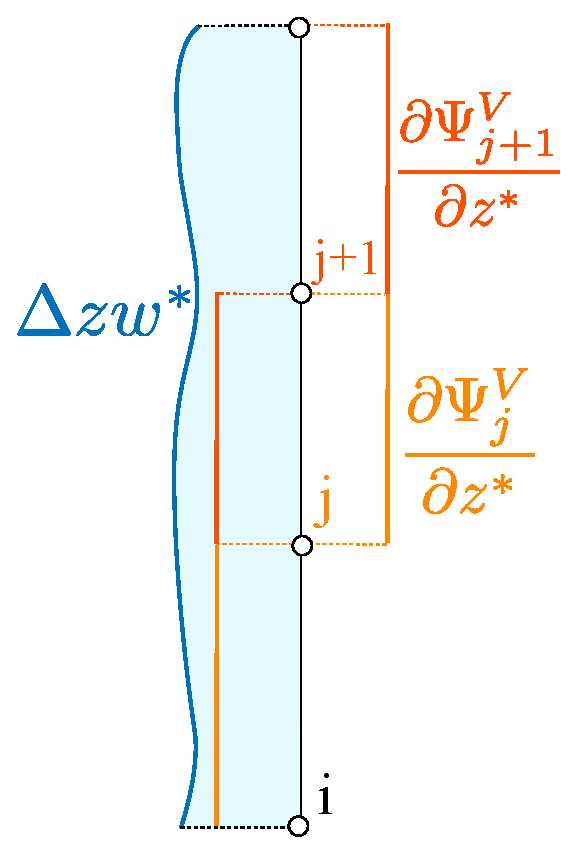
\includegraphics[scale=0.5]{graphics/fluvert.pdf}
\end{center}
\caption{Sketch of the cancellation of $\displaystyle{\sum_{j~above~i}}\displaystyle{\int_{\Omega^{\ast}}}\Delta zw^{\ast}
(\partial\Psi_{j}^{v\ast}/\partial z^{\ast})\Psi_{i}^{h}~d\Omega^{\ast}$: the
integral above a point $j$ cancels out with the one below $j+1$. The sum on
the whole vertical is thus equal to zero.}
\label{fig:fluvert}
\end{figure}
Indeed, the integrals cancel each other when summed along the vertical,
as shown in the figure \ref{fig:fluvert}.
The integration on the vertical of the equation \eqref{contidistr} thus reads:
\begin{equation}
\displaystyle{\int_{\Omega_{2D}}}\Psi_{i}^{h}\left(\dfrac{h^{n+1}-h^{n}}{\delta
t}\right)~d\Omega_{2D}+{\displaystyle\sum_{j~above~i}}
\left(-FLUINT(j)+FLUEXT(j)-SOURCE(j)\right)  =0
\end{equation}
or, more explicitely:%
\begin{equation}
\left[\begin{array}{l}
\displaystyle{\int_{\Omega_{2D}}}\Psi_{i}^{h}\left(\dfrac{h^{n+1}-h^{n}}{\delta
t}\right)~d\Omega_{2D}+
{\displaystyle\sum_{j~above~i}}FLUEXT(j)\\\bigskip
-\displaystyle{\sum_{j~above~i}}\int\nolimits_{\Omega^{\ast}}\Delta
z~\left(\theta_{u}\tilde{\vec{u}}^{n+1}+(1-\theta_{u})\vec{u}^{n}\right)\cdot\Grad^{\ast}\Psi_{j}^*~d\Omega^{\ast}
\end{array}\right]
={\displaystyle\sum_{j~above~i}}SOURCE(j)\label{eq:hequation}
\end{equation}

This corresponds to a variational formulation of the first
line of the equation \eqref{eq:hydrostatic_second_system}.

\begin{CommentBlock}{Remark:}
It is important to write a variational formulation and only then sum the integrals over the vertical,
otherwise the discrete conservation of mass is not achieved.
\end{CommentBlock}

\subsection{Estimation of the 2D conservative velocity}\label{momentumvariational}
In what follows, we want to obtain a formula to calculate $\tilde{\vec{u}}^{n+1}$ that
not involve having to solve a linear system: we need to then introduce
that formula into the equation \eqref{eq:hequation} to calculate $h^{n+1}$.
For this, we discretize the second line of the system \eqref{eq:wave_equation_time}, recalled below:
\begin{equation}
%  \dfrac{\tilde{\vec{u}}_{2D}^{n+1}-\vec{u}_{2D}^{A}}{\delta t}=-g \theta_h \Grad_{2D}(h^{n+1}-h^n) -g\Grad_{2D}\eta^n
%  + \tilde{\vec{F}}_{2D}
%  +\Div(\nu_E \Grad \vec{u}_{2D})
\dfrac{\vec{u}_{2D}^{aux}-\vec{u}_{2D}^{A}}{\delta t}= -g\Grad_{2D}\eta^n
     + \tilde{\vec{F}}_{2D}
     +\nu_E \Lap \vec{u}_{2D}\medskip\\
\end{equation}
Here the time discretisation of the diffusion term has not been specified: it is going to be specified below.
Recall that we then have:
\begin{equation}
 \tilde{\vec{u}}_{2D}^{n+1}=\vec{u}_{2D}^{aux}-g \theta_h \delta t\Grad_{2D}(h^{n+1}-h^n)
\end{equation}
We leave the framework of Finite Elements in this section, since we do not
write a variational formulation of the equation but rather use or compute nodal
values of each term so as to obtain $\vec{u}_{2D}^{aux}$ and then $\tilde{\vec{u}}_{2D}^{n+1}$.
The gradient term $-g\theta_{h}\Grad_{2D}(h^{n+1}-h^{n})$,
written also $-g\theta_{h}\Grad_{2D}\delta h$, shall be kept
in this continuous form when being introduced in the depth-integrated continuity equation.
When necessary, the nodal values of the fields or their gradients are estimated
with the following formula:
\begin{equation}
\left[f\right]_i\approx\dfrac{\displaystyle{\int_\Omega} f\Psi_i~d\Omega}{\displaystyle{\int_\Omega}\Psi_i~d\Omega}\label{eq:nodalvalue}
\end{equation}
or for a 2D field:
\begin{equation}
\left[f\right]_i\approx\dfrac{\displaystyle{\int_{\Omega_{2D}}}f\Psi_i~d\Omega_{2D}}{\displaystyle{\int_{\Omega_{2D}}}\Psi_i~d\Omega_{2D}}\label{eq:nodalvalue2D}
\end{equation}
Note that this is only an approximation of the nodal value of $f$.
Using this technique for the diffusion term yields:
\begin{equation}
\dfrac{\displaystyle{\int_{\Omega}}\Div(\nu_{E}\Grad\vec{u})\Psi_{i}~d\Omega}
{\displaystyle{\int_{\Omega}}\Psi_{i}~d\Omega}
\end{equation}
a form in which the discretisation in time is still not specified since we
wish to retain the friction terms in an implicit form and the volumic term in an
explicit, semi-implicit or implicit form.
An integration by parts of the numerator yields:
\begin{equation}
\displaystyle{\int_{\Omega}}\Div(\nu_{E}\Grad\vec{u}_{2D})\Psi_{i}~d\Omega=
\displaystyle{\int_{\Gamma}}\Psi_{i}\nu_{E}\Grad\vec{u}_{2D}\cdot\vec{n}~d\Gamma-
\displaystyle{\int_{\Omega}}\nu_{E}\Grad\vec{u}_{2D}\cdot\Grad\Psi_{i}~d\Omega
\end{equation}
Let us consider that the volumic
term is treated explicitly for the sake of simplicity.
The boundary term is treated implicitely.
The above equation then becomes:
\begin{equation}
\displaystyle{\int_{\Omega}}\Div(\nu_{E}\Grad\vec{u}_{2D})\Psi_{i}~d\Omega\simeq
\displaystyle{\int_{\Gamma}}\Psi_{i}\nu_{E}\Grad\vec{u}_{2D}^{aux}\cdot\vec{n}~d\Gamma
-\displaystyle{\int_{\Omega}}\nu_{E}\Grad\vec{u}_{2D}^{n}\cdot\Grad\Psi_{i}~d\Omega
\end{equation}
Now to deal with $\nu_{E}\Grad\vec{u}_{2D}^{aux}\cdot\vec{n}$ we write that:
\begin{equation}
\nu_{E}\Grad u^{aux}\cdot\vec{n}=aubor~u^{aux}+bubor
\end{equation}
and:
\begin{equation}
\nu_{E}\Grad v^{aux}\cdot\vec{n} = avbor~v^{aux}+bvbor
\end{equation}
$avbor=aubor$ represents the stress due to friction and $bubor$ and $bvbor$ an
explicit stress due for example to wind at the free surface or any other
stress at the bed or the lateral boundaries.
The term $\int_{\Gamma}\Psi_{i}\nu_{E}\Grad\vec{u}_{2D}^{aux}\cdot\vec{n}~d\Gamma$
finally takes the form of a diagonal matrix multiplied
by the velocity vector plus an explicit stress denoted by $\vec{bubor}$,
with components $bubor$ and $bvbor$. We now
estimate the nodal value of $aubor~\vec{u}_{2D}^{aux}$ with the formula
\eqref{eq:nodalvalue} and define $fric3d$ as:
\begin{equation}
\dfrac{\displaystyle{\int_{\Gamma}}\Psi_{i}~aubor~\vec{u}_{2D}^{aux}~d\Gamma}
{\displaystyle{\int_{\Omega}}\Psi_{i}~d\Omega}=-fric3d~\vec{u}_{2D}^{aux}
\end{equation}
We then use mass-lumping on $fric3d$ so as to have:
\begin{equation}
fric3d\simeq-\dfrac{\displaystyle{\int_{\Gamma}}\Psi_{i}~d\Gamma}
{\displaystyle{\int_{\Omega}}\Psi_{i}~d\Omega} aubor =
-\dfrac{aubor}{cos(\alpha)}~\dfrac{\displaystyle{\int_{\Omega_{2D}}}\Psi_{i}^{h}~d\Omega_{2D}}
{\displaystyle{\int_{\Omega}}\Psi_{i}~d\Omega}%
\end{equation}

Indeed, $1/cos(\alpha)$ is equal to $\sqrt{1+\left(\partial b/\partial x\right)^{2}+\left(\partial b/\partial y\right)^{2}}$
and as a matter of fact, we have:
\begin{equation}
d\Gamma=\sqrt{1+\left(\dfrac{\partial b}{\partial x}\right)^{2}
+\left(\dfrac{\partial b}{\partial y}\right)^{2}}d\Omega_{2D}
\end{equation}
on the bed, because the 2-dimensional domain is flat, whereas there is a
slope of the 2-dimensional boundary of the 3-dimensional domain.
On the other hand, we estimate the nodal value of $\nu_{E}\Grad\vec{u}_{2D}^{n}$
with the formula \eqref{eq:nodalvalue} and define $\vec{diff}$ as:
\begin{equation}
\vec{diff}=\dfrac{\displaystyle{\int_{\Omega}}\nu_{E}\Grad\vec{u}_{2D}^{n}
\cdot\Grad\Psi_{i}~d\Omega}{\displaystyle{\int_{\Omega}}\Psi_{i}~d\Omega}
-\vec{bubor}\dfrac{\displaystyle{\int_{\Gamma}}\Psi_{i}~d\Gamma}
{\displaystyle{\int_{\Omega}}\Psi_{i}~d\Omega}
\end{equation}
The nodal values of $\vec{bubor}$ were also approximated and a mass-lumping
was used to extract it from the integral, like for $\vec{aubor}$.
Finally, we estimate the diffusion term as:
\begin{equation}
\dfrac{\displaystyle{\int_{\Omega}}\Div(\nu_{E}\Grad\vec{u}_{2D})\Psi_{i}~d\Omega}
{\displaystyle{\int_{\Omega}}\Psi_{i}~d\Omega}\approx
-fric3d~\vec{u}_{2D}^{aux}-\vec{diff}
\end{equation}
%The expression of $\vec{u}^{C}$ carried over in the mass
%conservation equation will be:
%\begin{equation}
%\vec{u}^{C}=D^{-1}\left(\vec{u}^{A}+\delta t\left[-g\theta_{h}\Grad\delta h-g\Grad\eta^{n}
%-\dfrac{1}{\rho}\Grad p_{d}+\vec{F}-\vec{diff}\right]\right)
%\label{finalvel}
%\end{equation}

The expression of $\tilde{\vec{u}}_{2D}^{n+1}$ to be injected in the equation
\eqref{eq:hequation} then reads:
\begin{equation}
\tilde{\vec{u}}_{2D}^{n+1}=D^{-1}\left(\vec{u}_{2D}^{A}+\delta t\left[-g\theta_{h}\Grad_{2D}
\delta h^{n+1}+\dfrac{\displaystyle{\int_{\Omega_{2D}}}[-g\Grad_{2D}\eta^{n}]
\Psi_{i}^{h}~d\Omega_{2D}}{\displaystyle{\int_{\Omega_{2D}}}\Psi_{i}^{h}~d\Omega_{2D}}
+\vec{P}_{2D}+\vec{F}_{2D}-\vec{diff}\right]\right)\label{eq:uc}
\end{equation}
%while after the calculation of $\delta h$, $\vec{u}_{2D}^{C}$ is calculated
%through the formula:
%\begin{equation}
%\vec{u}_{2D}^{C}=D^{-1}\left(\vec{u}_{2D}^{A}+\delta t\left[
%\dfrac{\displaystyle{\int_{\Omega_{2D}}}[-g\theta_{h}\Grad_{2D}\delta h-g\Grad_{2D}
%\eta^{n}]\Psi_{i}^{h}d\Omega_{2D}}{\displaystyle{\int_{\Omega_{2D}}}\Psi_{i}^{h}
%d\Omega_{2D}}+\vec{P}_{2D}+\vec{F}_{2D}-\vec{diff}\right]\right)\label{eq:uc}
%\end{equation}
with:
\begin{equation}
D=1+\delta t(fric3d+s1u)
\end{equation}
with the explicit treatment of the volumic integral for the diffusion term, we have:
\begin{equation}
D^{-1}=\dfrac{1}{1+\delta t(fric3d+s1u)}%
\end{equation}
but it is intentionally kept in the form $D^{-1}$ because $D$ will become a
matrix when an implicit diffusion is taken into account (see the Finite Elements
discretisation of the diffusion step described in the equation \eqref{eq:diff}
for a better understanding of the implicit treatment of the diffusion).
$\vec{P}_{2D}$ stands for $-\int_{\Omega}1/\rho\Grad_{2D} p_{d}\Psi_{i}~d\Omega$.
%\textcolor{red}{Not divided by a psi integral??}
%We thus have an equation for the calculation of $\vec{u}^{C}$.

In the equation \eqref{eq:uc}, $\Grad_{2D}\delta h^{n+1}$ is calculated as
a nodal value, like $-g\,\Grad_{2D}\eta^{n}$, that is:%
\begin{equation}
\dfrac{\displaystyle{\int_{\Omega_{2D}}}[-g\theta_{h}\Grad_{2D}\delta
h^{n+1}-g\Grad_{2D}\eta^{n}]\Psi_{i}^{h}~d\Omega_{2D}}
{\displaystyle{\int_{\Omega_{2D}}}\Psi_{i}^{h}~d\Omega_{2D}}
\end{equation}
This is provisional, we will see in the next subsection that in the continuity
equation $\Grad_{2D}\eta^{n}$ can be treated differently suppress wiggles.

%Assuming that an advection step (explicit or method of characteristics) has
%earlier given a velocity field $\vec{u}^{C}$ the momentum equation is:%
%
%\begin{equation}
%\dfrac{\vec{u}^{n+1}-\vec{u}^{C}}{\delta t}%
%=-s1u\,\,\vec{u}^{n+1}-g\,\Grad(\eta)-\dfrac
%{1}{\rho}\Grad(p_{d})+\vec{F}+div(\nu
%_{t}grad(\vec{u}))
%\end{equation}
%
%where $\vec{F}$ specifically contains the buoyancy terms, that is:%
%
%\begin{equation}
%\vec{F}=g\dfrac{\Delta\rho}{\rho_{o}}\Grad%
%(\eta)-g\,\Grad\left(  \int\nolimits_{z}^{\eta}\dfrac
%{\Delta\rho}{\rho_{o}}dz^{\prime}\right)
%\end{equation}
%
%The term $-s1u\,\,\vec{u}^{n+1}$represents the manner in which any
%possible implicit source terms are treated. $s1u$ is a function discretised as
%the velocity.


\subsection{Variational formulation of the equation on $h^{n+1}$ - pseudo wave equation}

We have defined:
\begin{equation}
\vec{u}^{aux}=D^{-1}\left(\vec{u}_{2D}^{A}+\delta t\left[-
\dfrac{\displaystyle{\int_{\Omega_{2D}}}g\Grad_{2D}\eta^{n}\Psi_{i}^{h}~d\Omega_{2D}}
{\displaystyle{\int_{\Omega_{2D}}}\Psi_{i}^{h}~d\Omega_{2D}}
+\vec{P}_{2D}+\vec{F}_{2D}-\vec{diff}\right]\right)\label{UAUX}
\end{equation}
The depth-integrated continuity equation in variational formulation is then written as:
\begin{equation}
\begin{array}{l}
\displaystyle{\int_{\Omega_{2D}}}\Psi_{i}^{h}\left(\dfrac{h^{n+1}-h^{n}}{\delta t}\right)~d\Omega_{2D}
+g\delta t\theta_{h}\theta_{u}\displaystyle{\sum_{j~above~i}}
\left(\displaystyle{\int_{\Omega^{\ast}}}\Delta z~D^{-1}\Grad(h^{n+1}-h^{n})\cdot\Grad\Psi_{j}^{*}~d\Omega^{\ast}\right)=\\\medskip
\displaystyle{\sum_{j~above~i}}
\left(\displaystyle{\int_{\Omega^{\ast}}}\Delta z~
\left(\theta_{u}\vec{u}^{aux}+(1-\theta_{u})\vec{u}^{n}\right)
\cdot\Grad\Psi_{j}^{*}~d\Omega^{\ast}\right)+\displaystyle{\sum_{j~above~i}}\left[  SOURCE(j)-FLUEXT(j)\right]
\end{array}
\end{equation}
where the variational formulation for the term containing $\delta h$ in the conservative velocity is
now consistent with the rest of the water-depth equation -- a 3D integration followed by a summation on
the vertical of each degree of freedom.
The second term in the left-hand side is written as:
\begin{equation}
\begin{array}{l}
g\delta t\theta_{h}\theta_{u}\displaystyle{\sum_{j~above~i}}
\left(\displaystyle{\int_{\Omega^{\ast}}}\Delta z~D^{-1}\Grad(h^{n+1}-h^{n})\cdot\Grad\Psi_{j}^{*}~d\Omega^{\ast}\right)=%\\\bigskip
%g\delta t\theta_{h}\theta_{u}
%\displaystyle{\int_{\Omega_{2D}}}\left(\displaystyle{\sum_{j~above~i}}\Delta z~D^{-1}\right)\Grad(h^{n+1}-h^{n})\cdot\Grad\Psi_{i}^{h}d\Omega^{\ast}=%\\\bigskip
\displaystyle{\int_{\Omega_{2D}}}\nu_{wave}\Grad(h^{n+1}-h^{n})\cdot\Grad\Psi_{i}^{h}~d\Omega^{\ast}
\end{array}
\end{equation}
%\bigskip The term:%
%\begin{equation}
%\int_{\Omega^*}\left[\delta tD^{-1}g\theta_{h}\theta_{u}\Grad(h^{n+1}-h^{n})\right] \cdot
%\Grad\Psi_{i}^{h}d\Omega^*
%\end{equation}
%is written:%
%\begin{equation}
%\int\nolimits_{\Omega_{2D}}\nu_{wave}~\Grad(h^{n+1}%
%-h^{n})\,.\Grad(\Psi_{i}^{h})\,d(\Omega_{3D})
%\end{equation}
where $\nu_{wave}$ is a piece-wise constant function equal to:%
\begin{equation}
\nu_{wave}(ielem)=g\delta t~\theta_{h}\theta_{u}\sum_{prisms~above~ielem}
\overline{(\Delta zD^{-1})} \label{nuwave}%
\end{equation}
where the bar stands for an average on the prism. $ielem$ is a 2D element
number.

\begin{CommentBlock}{Remark:}
The choice of $\nu_{wave}$ as a piece-wise constant function stems
from the fact that when summed over the vertical, the terms:%
\begin{equation}
\sum_{j~above~i}\int_{\Omega^{\ast}}\Delta zg\delta t
\theta_{h}\theta_{u}D^{-1}\Grad(h^{n+1}-h^{n})\cdot\Grad\Psi_{j}^*~d\Omega^{\ast}
\end{equation}
should give:
\begin{equation}
\int_{\Omega_{2D}}\nu_{wave}\Grad(h^{n+1}-h^{n})\cdot\Grad\Psi_{i}^{h}~d\Omega_{2D}
\end{equation}
In this way the treatment of this term is simpler and we
recover a Saint-Venant like continuity equation.
If we consider the integral:
\begin{equation}
\int_{\Omega^{\ast}}\Delta z~g\delta t\theta_{h}\theta_{u}D^{-1}\Grad(h^{n+1}-h^{n})
\cdot\Grad\Psi_{j}^{*}~d\Omega^{\ast}
\end{equation}
on a prism, the only real 3-dimensional function is $\Delta z~D^{-1}$, so that
$\Delta z~D^{-1}$ can be replaced by its average on the prism $\overline
{\Delta z~D^{-1}}$ without changing the result. Then by summing over the
vertical we get to:
\begin{equation}
\int_{\Omega_{2D}}\nu_{wave}\Grad(h^{n+1}-h^{n})\cdot\Grad\Psi_{i}^{h}~d\Omega_{2D}
\end{equation}
%if we take $\nu_{wave}$ defined by the equation \ref{nuwave}.
\end{CommentBlock}


Finally, the variational formulation of the equation on $h^{n+1}$ reads:%
\begin{equation}
\begin{array}{l}
\displaystyle{\int_{\Omega_{2D}}}\left(\dfrac{h^{n+1}-h^{n}}{\delta t}\right)\Psi_{i}^{h}~d\Omega_{2D}
+\displaystyle{\int_{\Omega_{2D}}}\nu_{wave}\Grad(h^{n+1}-h^{n})\cdot\Grad\Psi_{i}^{h}~d\Omega_{2D}=\bigskip\\
\displaystyle{\sum_{j~above~i}}\left(\displaystyle{\int_{\Omega^{\ast}}}
\Delta z (\theta_{u}\vec{u}^{aux}+(1-\theta_{u})\vec{u}^{n})\cdot\Grad\Psi_{j}^{*}~d\Omega^{\ast})\right)
+\displaystyle{\sum_{j~above~i}}\left(  SOURCE(j)-FLUEXT(j)\right)
\end{array}
\label{contiwave}%
\end{equation}
and $\vec{u}_{2D}^{C}$ is calculated through:
\begin{equation}
\vec{u}_{2D}^{C}=\theta_u\vec{u}_{2D}^{aux}+(1-\theta_u)\vec{u}_{2D}^n
\label{eq:ucfinal}
\end{equation}
%and the variational formulation of the momentum equation is:%
%\begin{equation}
%\vec{u}_{2D}^{C}=\vec{u}^{aux}-\delta tD^{-1}\left[
%\dfrac{\int_{\Omega_{2D}}g\theta_{h}\Grad_{2D}(h^{n+1}-h^{n})\Psi_{i}^{h}d\Omega_{2D}}
%{\int_{\Omega_{2D}}\Psi_{i}^{h}d\Omega_{2D}}\right] \label{finalvelocity}%
%\end{equation}

%\clearpage
%%%%%%%%%%%%%%%%%%%%%%%%%%%%%%%%%%%%%%%%%%%%%%%%%%%%%%%%%%%%%%%
\begin{CommentBlock}{Remark:}
In case the gradient of the dynamic pressure is included in $\vec{u}^{aux}$,
a term $-(1/\rho)\Grad p_{d}$ is added to
the momentum equation, where $p_{d}$ is calculated by applying the Chorin
projection method before calculating the new water depth.
This corresponds to the key-word \texttt{DYNAMIC PRESSURE IN WAVE EQUATION}
(see the section \ref{sec:dynamicpressureinwaveequation}).
\end{CommentBlock}
%%%%%%%%%%%%%%%%%%%%%%%%%%%%%%%%%%%%%%%%%%%%%%%%%%%%%%%%%%%%%%%
\\

%%%%%%%%%%%%%%%%%%%%%%%%%%%%%%%%%%%%%%%%%%%%%%%%%%%%%%%%%%%%%%%
\begin{CommentBlock}{Some history:}
In former versions of TELEMAC-3D this step was solved by
calling TELEMAC-2D. It then appeared that this was a theoretical
mistake: average on the vertical and discretisation do not commute. The right
thing to do is to first discretise the equations in 3D, then to sum them over
the vertical. This sum is thus discrete and done plane by plane. In the more
recent versions the only technique proposed is the wave equation, which
consists of eliminating the velocity from the depth-summed continuity equation,
yielding an equation on the depth, which looks like a wave equation as the celerity
of waves clearly appears in it.
\end{CommentBlock}

\subsubsection{Equivalence between the pseudo-wave equation and a Saint-Venant like continuity equation}
The continuity equation, given bed and free-surface boundary conditions,
yields a Saint-Venant like continuity equation. The classical version of the
Saint-Venant continuity equation is recalled below, with a variational formulation and a time discretisation:
\begin{equation}
\displaystyle{\int_{\Omega_{2D}}}\left(\dfrac{h^{n+1}-h^{n}}{\delta t}
\right)\Psi_{i}^{h}~d\Omega_{2D}
+\displaystyle{\int_{\Gamma_{2D}}}h\vec{U}\cdot\vec{n}\Psi_{i}^{h}~d\Gamma_{2D}
-\displaystyle{\int_{\Omega_{2D}}}h\vec{U}\cdot\Grad\Psi_{i}^{h}~d\Omega_{2D}=0
\end{equation}
The continuity equation solved to obtain the values of water height,
\eqref{contiwave}, can also be considered as:%
\begin{equation}
\begin{array}{l}
\displaystyle{\int_{\Omega_{2D}}}\left(\dfrac{h^{n+1}-h^{n}}{\delta t}
\right)\Psi_{i}^{h}~d\Omega_{2D}-\displaystyle{\sum_{j~above~i}}\left(
\displaystyle{\int_{\Omega^{\ast}}}\Delta z\vec{u}^{comp}\cdot\Grad\Psi_{j}^{*}
~d\Omega^{\ast}\right)\bigskip\\
-\displaystyle{\sum_{j~above~i}}\left(  SOURCE(j)-FLUEXT(j)\right)  =0
\end{array}
\end{equation}
with $\vec{u}^{comp}$ being here:
\begin{equation}
\vec{u}^{comp}=\theta_u\vec{u}^{aux}+(1-\theta_u)\vec{u}^n-g\delta t\theta_{h}\theta_{u}D^{-1}\Grad(h^{n+1}-h^{n})%=\theta_u\vec{u}^{C*}+(1-\theta_u)\vec{u}^n
\end{equation}
We have:
\begin{equation}
\displaystyle{\sum_{j~above~i}}\left(
\displaystyle{\int_{\Omega^{\ast}}}\Delta z\vec{u}^{comp}\cdot\Grad\Psi_{j}^{*}
~d\Omega^{\ast}\right)=\int_{\Omega_{2D}}\displaystyle{\sum_{j~above~i}}\Delta z\vec{u}^{comp}\cdot\Grad\Psi_j^H~d\Omega_{2D}
\end{equation}
For the same reason as $FLUEXT = 0$, so that the equation \eqref{contiwave}
is a form of depth-integrated continuity equation, as expected.

\subsubsection{Mass-lumping of the pseudo-wave equation}\label{sec:masslumping}

Mass-lumping may be used to solve the pseudo-wave equation.
It is always the case when distributive schemes are used for the advection,
otherwise it is a choice left to the user.
In case mass-lumping is used, the left-hand side of the equation
\eqref{contiwave} is approximated in the form:
\begin{equation}
\dfrac{1}{\delta t}\int\nolimits_{\Omega_{2D}}(h^{n+1}-h^{n})\Psi_{i}^{h}
~d\Omega_{2D}\simeq\dfrac{(h_{i}^{n+1}-h_{i}^{n})}{\delta t}\int%
\nolimits_{\Omega_{2D}}\Psi_{i}^{h}~d\Omega_{2D}%
\end{equation}
then the terms $\int\nolimits_{\Omega^{n+1}}\Psi_{i}~d\Omega^{n+1}$ and
$\int\nolimits_{\Omega^{n}}\Psi_{i}~d\Omega^{n}$ must be modified accordingly
everywhere they are used in the equations. Indeed, for a case like the one
shown in the figure \ref{fig:masslumping}, the integral of the basis
around $i$ is not equal to zero while $h_i$ is equal to 0, so that the
mass-lumped terms involving $h_i$ will cancel out but not the ones
involving other quantities. This leads to spurious mass transfers and must be avoided. As a matter of fact, we must write:%
\begin{equation}
\int\nolimits_{\Omega}\Psi_{i}~d\Omega=\int_{\Omega^{\ast}}h\Psi_{i}^{\ast
}~d\Omega^{\ast}\simeq h_{i}\int_{\Omega^{\ast}}\Psi_{i}^{\ast}~d\Omega^{\ast}%
\label{eq:volu}
\end{equation}
In this way, the calculation the diffusion stage (for the vertical velocity and
scalars) and the velocity correction stage remain compatible
with the mass-lumped pseudo wave equation.

\begin{figure}
\begin{center}
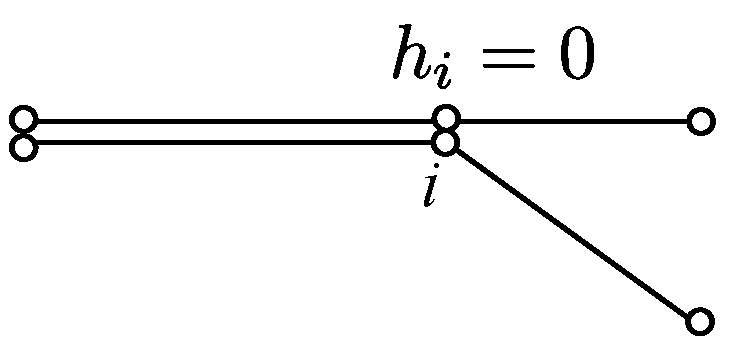
\includegraphics[scale=0.5]{graphics/masslumping.pdf}
\end{center}
\caption{Sketch of a configuration where mass-lumping would lead to an
incompatibility between the pseudo wave equation and the calculation
of $\Delta zw^{C*}$ without a specific treatment of the terms $\int\nolimits_{\Omega}\Psi_{i}~d\Omega$ in the equations.}\label{fig:masslumping}
\end{figure}

\begin{CommentBlock}{Remark:}
This corresponds to the calculation of \texttt{VOLU} with the formula
\texttt{MASBAS 2} in the subroutine \texttt{vc00pp.f}.
\end{CommentBlock}

\subsection{Suppressing wiggles: compatibility of the free surface gradient}

In the equation \eqref{eq:uc} used to calculate $\vec{u}^{aux}$,
the explicit free surface gradient is a linear function taken as:
\begin{equation}
\Grad\eta^{n}_{linear}\simeq\dfrac{{\displaystyle\int_{\Omega}}
\Grad\eta^{n}\Psi_{i}~d\Omega}{{\displaystyle\int_{\Omega}}
\Psi_{i}~d\Omega}
\end{equation}
for every degree of freedom $i$ with test function $\Psi_{i}$. This is the
"compatible" way of computing the gradient. Oscillations of $\eta$ are
not "seen" by this way of discretising the gradient and do not
trigger a velocity that would
cause artificial maxima of free-surface elevation to smooth out.
To damp such spurious oscillations, $\Grad\eta^{n}$ should be considered as a
piece-wise constant function, in a way consistant with the fact
that $\eta^{n}$ is a linear function. This is the "non compatible way"
of computing the gradient.

%However, oscillations of $\eta$ are not "seen" by this way of
%discretising the gradient and do not trigger a velocity that would
%cause artificial maxima of free-surface elevation to smooth out.
%To damp such spurious oscillations, $\Grad\eta^{n}$ should be considered as a
%piece-wise constant function, in a way consistant with the fact
%that $\eta^{n}$ is a linear function. This is the "non compatible way"
%of computing the gradient.
%In the wave equation routine of TELEMAC-3D,
%it happens that $\eta$ is written as:
%\begin{equation}
%\eta=\eta^{n}+\theta_{h}(h^{n+1}-h^{n})
%\end{equation}
%If we look at the equation \ref{contiwave} we see that the increment of depth is
On the other hand, the terms involving $\Grad(h^{n+1}-h^{n})$ in
\eqref{contiwave} are
piece-wise constant functions, since they are the gradients of a piece-wise
linear function. This is the ``non-compatible'' way of discretising the
free-surface gradient.
%These two manners to discretise the water depth are called the ``compatible''
%and ``non compatible'' discretisations.
The ``compatible'' way of discretising $\Grad\eta^n$
makes it possible to obtain a velocity field such as
\mbox{$\partial h/\partial t+\Div(h\vec{u})=0$} is fulfilled.
However, with this discretisation, oscillations of $\eta$ are invisible
because they do not trigger a velocity that would
cause artificial maxima of free-surface elevation to smooth out.
The ``non-compatible'' way of discretising $\eta$ helps
smoothing out spurious oscillations but the velocity field
does not exactly obey the continuity equation anymore.\\
%To damp such spurious oscillations, $\Grad\eta^{n}$ can be considered as a
%piece-wise constant function, in a way consistant with the fact
%that $\eta^{n}$ is a linear function. This is the "non compatible way"
%of computing the gradient.
%treated in a non compatible way because it ends up in the term:
%\begin{equation}
%\int_{\Omega_{2D}}\nu_{wave}\Grad(h^{n+1}-h^{n})\cdot\Grad\Psi_{i}^{h}d\Omega_{2D}
%\end{equation}
%where $\Grad(h^{n+1}-h^{n})$ is naturally taken as a
%piece-wise constant function, whereas the explicit part $\eta^{n}$ is
%treated in a compatible way to give $\vec{u}^{aux}$ through the equation
%\eqref{UAUX}.

To sum up, a totally compatible $\Grad\eta$ ensures
a better compatibility of the continuity equation with the velocity field,
%in the sense that we would be
%able to show a velocity $\vec{u}$ so as
%\mbox{$\dfrac{\partial h}{\partial t}+\Div(h\vec{u})=0$}.
while a totally non compatible $\Grad\eta$ makes it
possible to suppress spurious oscillations of the free-surface elevation.
It happens that the non compatible treatment of $\Grad(h^{n+1}-h^{n})$ is
not always sufficient to suppress spurious oscillations, hence the
idea of treating also the term $\Grad \eta^{n}$ in a non-compatible way.
This can be achieved by suppressing $\Grad \eta^{n}$ in the computation
of $\vec{u}^{aux}$ (equation \eqref{UAUX}), and adding the following term to
the right hand side of the continuity equation:
\begin{equation}
-\int_{\Omega_{2D}}\dfrac{\nu_{wave}}{\theta_{h}}\left[\Grad\eta^{n}\right]_{piece-wise~const.}\cdot\Grad\Psi_{i}^{h}~d\Omega_{2D}
\end{equation}
Suppressing $\Grad\eta^{n}$ in the computation of $\vec{u}^{aux}$
is actually equivalent to adding:
\begin{equation}
-\int_{\Omega}\dfrac{\nu_{wave}}{\theta_{h}}\left[\Grad\eta^{n}\right]_{linear}
\cdot\Grad\Psi_{i}^{h}~d\Omega
\end{equation}
to the right-hand side of the continuity equation. The two terms do not sum to
zero because $\Grad\eta^{n}$ is not discretised in the same
way. With a parameter $\theta^{comp}$ varying from 0 to
1 we can skip from compatible to non compatible $\Grad\eta^{n}$.
%\textcolor{red}{The figure \ref{figure1} shows the effect of a choice of
%$\theta^{comp}$=0.9 in the case of a flow around bridge piers. Wiggles are
%clearly suppressed.}
When recovering the final velocity with the formula
\eqref{eq:ucfinal}, one must not forget that $\vec{u}^{aux}$ lacks
the non compatible part of the free surface gradient, hence this lacking part
must be added, and it can only be done in a compatible way to get a
linear contribution.\\

\begin{CommentBlock}{Remark:}
When $\Grad\eta^{n}$ is referred to in the formulae, care must
be taken that in the case of tidal flats with treatment by option 1
(correction of the free surface), the function $\eta^{n}$ is piece-wise linear
and must be stored in a specific array. BIEF subroutines must be written in
order to deal with such a discretisation.
\end{CommentBlock}


\section{Space discretisation of the pressure step}

We recall that in this step the following equations are solved:
\begin{equation}
  \left\{\begin{array}{l}
    \Lap p_d^{n+1} = \dfrac{\rho}{\delta t}\Div \tilde{\vec{u}}^{n+1} \medskip \\
    \dfrac{\vec{u}^{n+1}-\tilde{\vec{u}}^{n+1}}{\delta t} = -\dfrac{1}{\rho}\Grad p_d^{n+1}
  \end{array}\right.\label{eq:pressurestepdiscrete}
\end{equation}
where $\tilde{\vec{u}}^{n+1}$ denotes the non divergence-free vector of components
$(u^C, v^C, w^D)$ (see the chapter \ref{Chapter3}).
The variational formulation is written as:%
\begin{equation}
\int_{\Omega}\Div\left(\dfrac{\delta t}{\rho}\Grad p_{d}\right)\Psi_{i}~d\Omega =
\int_{\Omega} \Div\vec{\widetilde{u}}^{n+1}\Psi_{i}~d\Omega
\end{equation}
The left-hand side of this equation is integrated by parts:
\begin{equation}
\int_{\Gamma}\Psi_{i}\dfrac{\delta t}{\rho}\Grad p_{d}\cdot \vec{n}~d\Gamma
-\int_{\Omega}\dfrac{\delta t}{\rho}\Grad p_{d}\cdot\Grad \Psi_{i}~d\Omega
=\int_{\Omega}\Div\vec{\widetilde{u}}^{n+1}\Psi_{i}\,d\Omega
\end{equation}
which is also:%
\begin{equation}
\int_{\Omega}\dfrac{\delta t}{\rho}\Grad p_{d}\cdot \Grad\Psi_{i}~d\Omega =
\int_{\Gamma}\Psi_{i}\dfrac{\delta t}{\rho}\Grad p_{d} \cdot \vec{n}~d\Gamma
-\int_{\Omega}\Div\vec{\widetilde{u}}^{n+1}\Psi_{i}~d\Omega\label{basic}%
\end{equation}


and by admitting the condition $\partial p_{d}/\partial n=0$
as a wall boundary condition for $p_{d}$, we arrive at the system:%
\begin{equation}
\int_{\Omega}\dfrac{\delta t}{\rho}\Grad p_{d}^{n+1}\cdot\Grad\Psi_{i}~d\Omega =
-\int_{\Omega}\Div\vec{\widetilde{u}}^{n+1}\Psi_{i}~d\Omega\label{lapla}
\end{equation}
This is the Poisson equation. The matrix of this system is a diffusion-type
matrix built with 1 in the place of viscosity, the pressure found being in
fact $(\delta t/\rho)p_{d}$. The boundary condition on the free surface
is $p_{d}=0$.
%This is one of the reasons why the divergence of the velocity is
%not zero after the projection (equation \ref{lapla}\ is locally cancelled by
%the Dirichlet treatment).
Once $p_{d}^{n+1}$ is known, $\vec{u}^{n+1}$ is retrieved with the second line of
\eqref{eq:pressurestepdiscrete}, which is also subjected to a variational formulation:%
\begin{equation}
\displaystyle{\int_{\Omega}}\vec{u}^{n+1}\Psi_i~d\Omega
-\displaystyle{\int_{\Omega}}\vec{\widetilde{u}}^{n+1}\Psi_i~d\Omega=
-\dfrac{\delta t}{\rho}\displaystyle{\int_{\Omega}}\Grad p_{d}^{n+1}\Psi_{i}~d\Omega
\label{projec2}%
\end{equation}
which is discretised into:
\begin{equation}
\displaystyle{\int_{\Omega}}\vec{u}_j^{n+1}\Psi_j\Psi_i~d\Omega
-\displaystyle{\int_{\Omega}}\vec{\tilde{u}}_j^{n+1}\Psi_j\Psi_i~d\Omega=
-\dfrac{\delta t}{\rho}\displaystyle{\int_{\Omega}}
p_{dj}^{n+1}\Grad\Psi_{j}\Psi_i~d\Omega
\end{equation}
for all degrees of freedom $i$, $j$. In this equation, the pressure gradient
was discretised through:
\begin{equation}
\Grad p_{d}^{n+1}=\sum_j p_{dj}^{n+1}\Grad\Psi_{j}
\end{equation}
by deriving the discretised pressure, $p(x,y,z)=\sum_jp_j\Psi_j(x,y,z)$.
The two terms of the left-hand side are mass-lumped in TELEMAC-3D (there is no
option available yet to solve the full linear system), so that the velocity
$\vec{u}^{n+1}$ is calculated through:
\begin{equation}
\vec{u}_j^{n+1}=\vec{\tilde{u}}_j^{n+1}-\dfrac{\delta t}{\rho}
\dfrac{\displaystyle{\int_{\Omega}}p_{dj}^{n+1}\Grad\Psi_{j}\Psi_i~d\Omega}
{\displaystyle{\int_{\Omega}}\Psi_{j}~d\Omega}
\end{equation}
%This projection method is the weak point of the non-hydrostatic option. The
%detailed reasons and various possible improvements were pondered in reference
%\cite{release57}.
for all degrees of freedom $i$, $j$. The term $\displaystyle{\int_{\Omega}}
\Psi_{j}~d\Omega$ in the denominator of the right-hand side is calculated in
agreement with the choice of mass-lumping on the water-height term in the
wave equation: if mass-lumping was activated, it is calculated through the
equation \eqref{eq:volu}.

\section{\label{calcul de w}Computing the conservative vertical velocity}

The conservative vertical velocity $w^C$ is calculated on the basis of the
mass conservation equation.
%As pressure is assumed hydrostatic, $w$ is required only for the
%advection step at the next time step.
As the advection is executed in the fixed transformed mesh, it is actually
$w^{C\ast}$ that we ought to know. Indeed, $w^{C}$ is only used during the calculation
of the advection terms.

\begin{CommentBlock}{Remark:}
All the demonstrations of conservation of mass for the distributive
schemes were done considering that both the advection and the mass conservation equation
(both in the form of the wave equation and in its classical form to retrieve $w^C$),
are solved in the transformed mesh. They could be solved in the fixed mesh but
this would increase the complexity of the algorithm.
\end{CommentBlock}

%It is more judicious to solve the 3D mass conservation equation in a fixed mesh.
%Thus we avoid the to and fro movement between the real and fixed mesh which makes the
%calculation unwieldy.
In fact, except in the case of advection by the method of characteristics,
where $w^{C\ast}$ is really used, it is the $\Delta zw^{C\ast}$ grouping which
appears often and which is homogeneous to a velocity (we recall that $\Delta
z$ is the depth between two planes, see the section \ref{transformation sigma}).
The formula for passing from $w^{\ast}$ to $w$, i.e. $w=\Delta zw^{C\ast}$ +
other terms (see the equation \ref{WWSTAR} below, we treat here the generalized
sigma transform case), shows that $\Delta zw^{C\ast}$ should have the same
discretization as $w^C$. It appears that in the fixed mesh, the real unknown
should be $\Delta zw^{C\ast}$ and not $w^{C\ast}$. We shall now examine a method
for calculating $\Delta zw^{C\ast}$, then how $w^C$ is found on the basis of
$\Delta zw^{C\ast}$. We first have to establish the form of the continuity
equation in the transformed mesh.

\subsection{\label{continuitytransformed}Discretisation of the continuity equation}

We recall here the continuity equation $div(\vec{u}^C)=0$ written in
the transformed mesh (equation \ref{divutransf}):
\begin{equation}
\dfrac{1}{\Delta z}\left[  \dfrac{\partial\Delta z}{\partial t}+\left(
\dfrac{\partial\left(  \Delta zu^C\right)  }{\partial x}\right)  _{y,z^{\ast}%
,t}+\left(  \dfrac{\partial\left(  \Delta zv^C\right)  }{\partial y}\right)
_{x,z^{\ast},t}+\left(  \dfrac{\partial\Delta zw^{C\ast}}{\partial z^{\ast}%
}\right)  _{x,y,t}\right]=0 \label{continuiteparplan}
\end{equation}

For each degree of freedom $i$ we should thus solve:
\begin{equation}
\int_{\Omega^{\ast}}\left[  \dfrac{\partial\Delta z}{\partial t}+\left(
\dfrac{\partial\Delta zu^C}{\partial x}\right)  _{y,z^{\ast},t}+\left(
\dfrac{\partial\Delta zv^C}{\partial y}\right)  _{x,z^{\ast},t}+\left(
\dfrac{\partial\Delta zw^{C\ast}}{\partial z^{\ast}}\right)  _{x,y,t}\right]
\Psi_{i}^{\ast}\,d\Omega^{\ast}=0
\end{equation}

With a simple sigma transformation, we would in fact get:
\begin{equation}
\int_{\Omega^{\ast}}\left[\left(\dfrac{\partial h}{\partial t}\right)
_{x,y}+\left(\dfrac{\partial hu^C}{\partial x}\right)_{y,z^{\ast},t}+\left(
\dfrac{\partial hv^C}{\partial y}\right)_{x,z^{\ast},t}+\left(  \dfrac{\partial
hw^{C\ast}}{\partial z^{\ast}}\right)_{x,y,t}\right]  \Psi_{i}^{\ast
}~d\Omega^{\ast}=0
\end{equation}
where we see the underlying depth-integrated continuity equation.
It is actually this form of the mass conservation equation that is found while
demonstrating the mass conservation of the scalar (see the section
\ref{masse traceur}). Discretized as such, this equation whose unknown is
$w^{C\ast}$ or rather $\Delta zw^{C\ast}$ leads to a system that is
ill-conditioned. The boundary conditions are
$w^{C\ast}=0$ at the bed and the free surface, if they are impermeable. The term:%
\begin{equation}
\int_{\Omega^{\ast}}\left(  \dfrac{\partial\Delta zw^{C\ast}}{\partial z^{\ast}}\right)_{x,y,t}
\Psi_{i}^{\ast}~d\Omega^{\ast}%
\end{equation}
with the unknown $\Delta zw^{C\ast}$ leads to a matrix $A$ with general term:%
\begin{equation}
A_{ij}=\int_{\Omega^{\ast}}\dfrac{\partial\Psi_{j}^{\ast}}{\partial z^{\ast}%
}\Psi_{i}^{\ast}~d\Omega^{\ast}%
\end{equation}

Outside the boundaries, the diagonal terms of this matrix are zero and it is not
invertible. From the boundary conditions at the bed and the free surface, we arrive at
disconnected solutions between two successive planes (parasitic oscillations),
or an impossibility.
%This is because the only unknown retained for solving
%mass conservation is the vertical velocity. The figure \ref{probleme surcontraint}
%shows the case of a mesh reduced to two planes, where no degree of freedom is
%available on the vertical of a point $i$ to find a vertical velocity for re-establishing
%a divergence-free flow.%
%
%\begin{figure}[tbh]%
%\centering
%\includegraphics[scale=0.5]{graphics/fluxes_overconstrained.pdf}%
%\caption{Example of a forced problem.}%
%\label{probleme surcontraint}%
%\end{figure}
%
%A vertical velocity defined on a staggered mesh would be necessary, as in
%the figure \ref{vitesse verticale}.%
%\begin{figure}[tbh]%
%\centering
%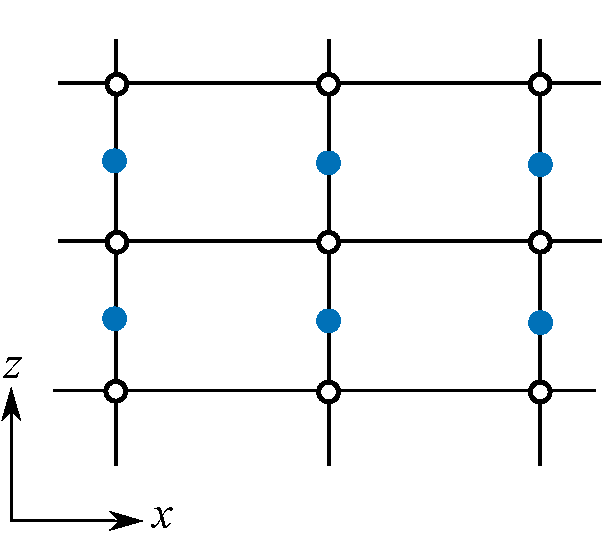
\includegraphics[scale=0.5]{graphics/fluxes.pdf}%
%\caption{Definition of a vertical velocity defined on a staggered mesh.}%
%\label{vitesse verticale}%
%\end{figure}
To circumvent this problem, a solution consists of changing unknowns or, to
be more precise, of giving a specific definition of the unknown $\Delta
zw^{C\ast}$. This definition, which will be given in the next paragraph, has
been inspired by the necessity to get an exact mass conservation of scalars
with distributive schemes. As a matter of fact, it will in due course appear
that this definition of $\Delta zw^{C\ast}$ is entirely compatible with these
distributive schemes.

\subsection{\label{wstarmoyen}Calculation of $\ \Delta zw^{C\ast}$:}

For each point $i$ of the mesh, the calculation of $\Delta zw^{C\ast}$ is done by solving:%
\begin{equation}
\int_{\Omega^{\ast}}\left(\Delta z^{n+1}-\Delta z^{n}\right)\Psi_{i}^{\ast}~d\Omega^{\ast}=
\delta t\int_{\Omega^{\ast}}\Delta z\vec{u}^C\cdot\Grad\Psi_{i}^{\ast}~d\Omega^{\ast}
-\delta t\int_{\Gamma^{\ast}}\Delta z\vec{u}^C\cdot\vec{n}\Psi_{i}^{\ast}~d\Gamma^{\ast}
\end{equation}
In the right-hand side, no time discretization of $\Delta z$ is specified yet.
Actually, it must be consistent with the 2D continuity equation, as will be
explained later, which generally imposes that $\Delta z$ is taken at time
$t^{n}$. We shall now show that the problem is well-posed if we consider that the
unknowns are the average of $\Delta zw^{C\ast}$ along the vertical of each prism.
This corresponds to a definition of the vertical velocity on a staggered mesh,
as represented in the figure \ref{vitesse verticale}.
\begin{figure}[tbh]%
\centering
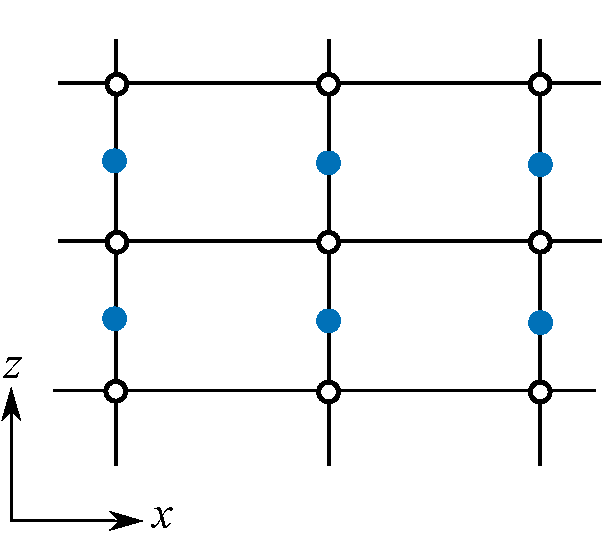
\includegraphics[scale=0.5]{graphics/fluxes.pdf}%
\caption{Definition of a vertical velocity on a staggered mesh: the blue dots represent
the degrees of freedom for the vertical velocity and the white dots represent the degrees
of freedom for the horizontal velocity.}%
\label{vitesse verticale}%
\end{figure}
Let us separate the horizontal and vertical gradients in the continuity
equation:
\begin{equation}
\begin{array}{ll}
\displaystyle{\int_{\Omega^{\ast}}}\Delta zw^{C\ast}\dfrac{\partial\Psi_{i}^{\ast}}{\partial
z^{\ast}}~d\Omega^{\ast} & =\dfrac{1}{\delta t}\displaystyle{\int_{\Omega^{\ast}}}\left(  \Delta
z^{n+1}-\Delta z^{n}\right)  \Psi_{i}^{\ast}~d\Omega^{\ast} \bigskip\\
& -\displaystyle{\int_{\Omega^{\ast}}}\Delta z\vec{u}^C\cdot\Grad_{2D}\Psi_{i}^{\ast}~d\Omega^{\ast}
+\displaystyle{\int_{\Gamma^{\ast}}}\Delta z\vec{u}^C\cdot\vec{n}\Psi_{i}^{\ast}~d\Gamma^{\ast}
\end{array}\label{CONT3D}
\end{equation}

In this form, the right-hand side only contains known terms (assuming that the
flux boundary conditions are given at the boundaries). So, we concentrate on
the left-hand side which contains unknowns. For this, it should be considered
that we work with prisms in the transformed fixed mesh, hence with horizontal
base and top. In these conditions, prisms are homothetic to the reference
prism and the 3D bases are products of one function of $x$ and $y$ and one
function of $z$ %(let us recall that for example $\Psi_{1}=(1-\alpha -\beta)\dfrac{(1-\gamma)}{2})$).
The function of $x$ and $y$ is the same as
the basis functions of triangles with linear interpolation. This makes it possible to
break down each basis as $\Psi_{i}^{\ast}=\Psi_{i}^{h}\Psi_{i}^{v}$ where $\Psi
_{i}^{h}$ only depends on $x$ and $y$, while $\Psi_{i}^{v}$ only depends on
$z$. Thus:%

\begin{equation}
\dfrac{\partial\Psi_{i}^{\ast}}{\partial z^{\ast}}=\Psi_{i}^{h}\dfrac
{\partial\Psi_{i}^{v}}{\partial z^{\ast}}%
\end{equation}

For any elevation $z^*$, we discretize the function $\Delta z\vec{u}^{C\ast}$ on the 2D domain as follows:%
\begin{equation}
\Delta z\vec{u}^{C\ast}=\sum\limits_{j=1}^{npoin2}\left[
\Delta z\vec{u}^{C\ast}(z^{\ast})\right]_{j}\Psi_{j}^{h}(x,y)
\end{equation}
where $npoin2$ is the number of degrees of freedom in the 2D mesh.

\begin{WarningBlock}{Remark:}
This choice is very impacting and constitutes a decorrelation of
the layers with regards to the vertical velocity.
%It comes to considering that the values of $\Delta z w^{C\ast}$ on each layer
%only depend on the values of the horizontal velocity above and below.
\end{WarningBlock}

%\textcolor{red}{$\Delta zw^{C\ast}(z^{\ast})$ is a function defined between 0 and 1 for each vertical line of nodes of the transformed mesh.}
The left-hand side of the equation \ref{CONT3D} then becomes:%
\begin{equation}
\sum_{j=1}^{npoin2}\left(\int_{\Omega_{2D}}\Psi_{i}^{h}\Psi_{j}^{h}~d\Omega_{2D}
\int_{0}^{1}\left[\Delta zw^{\ast}(z^{\ast})\right]_{j}\dfrac{\partial\Psi_{i}^{v}}
{\partial z^{\ast}}~dz^{\ast}\right)
\end{equation}
The mass matrix of the 2D mesh appears in $\int_{\Omega_{2D}}\Psi_{i}^{h}\Psi_{j}^{h}~d\Omega_{2D}$.
According to the position of the point $i$, the value of $\partial
\Psi_{i}^{v}/\partial z^{\ast}$ in a prism is equal to $\pm 1/\Delta z^{\ast}$,
where $\Delta z^{\ast}$ is the height of the prism (these bases
are linear; their value is 1 at the top and 0 at the bed or vice versa).

For a basis located on the plane $ip$, a plane different from the bed and
the free surface, we get:
\begin{equation}
\begin{array}{ll}
\displaystyle{\int_{0}^{1}}\left[  \Delta zw^{C\ast}(z^{\ast})\right]_{j}
\dfrac{\partial\Psi_{i}^{v}}{\partial z^{\ast}}~dz^{\ast}& =
\dfrac{1}{z_{ip}^{\ast}-z_{ip-1}^{\ast}}\displaystyle{\int_{z_{ip-1}^{\ast}}}^{z_{ip}^{\ast}}
\left[  \Delta zw^{C\ast}(z^{\ast})\right]_{j}~dz^{\ast}\\\bigskip
& -\dfrac{1}{z_{ip+1}^{\ast}-z_{ip}^{\ast}}\displaystyle{\int_{z_{ip}^{\ast}
}^{z_{ip+1}^{\ast}}}\left[  \Delta zw^{C\ast}(z^{\ast})\right]_{j}~dz^{\ast}
\end{array}
\end{equation}
The quantities retrieved here are the ones which help to calculate the
coefficients of distributive schemes (see the section
\ref{schema murd en dimension 3}).
Let us define:%
\begin{equation}
\overline{\left(  \Delta zw^{C\ast}\right)  }_{ip-\dfrac{1}{2}}^{j}=\dfrac
{1}{(z_{ip}^{\ast}-z_{ip-1}^{\ast})}\int\nolimits_{z_{ip-1}^{\ast}}%
^{z_{ip}^{\ast}}\left[  \Delta zw^{C\ast}(z^{\ast})\right]_{j}~dz^{\ast}%
\end{equation}
we finally get:%
\begin{equation}
\int\nolimits_{0}^{1}\left[\Delta zw^{C\ast}(z^{\ast})\right]_{j}
\dfrac{\partial\Psi_{i}^{v}}{\partial z^{\ast}}~dz^{\ast}=\overline{\left(
\Delta zw^{C\ast}\right)}_{ip-1/2}^{j}-\overline{\left(\Delta
zw^{C\ast}\right)}_{ip+1/2}^{j}%
\end{equation}

For a point located on the bed, we have:%
\begin{equation}
\int_{0}^{1}\,\left[  \Delta zw^{C\ast}(z^{\ast})\right]  _{j}%
\dfrac{\partial\Psi_{i}^{v}}{\partial z^{\ast}}~dz^{\ast}=+\overline{\left(
\Delta zw^{C\ast}\right)  }_{1+1/2}^{j}%
\end{equation}
and at the surface:%
\begin{equation}
\int_{0}^{1}\,\left[  \Delta zw^{C\ast}(z^{\ast})\right]  _{j}%
\dfrac{\partial\Psi_{i}^{v}}{\partial z^{\ast}}~dz^{\ast}=-\overline{\left(
\Delta zw^{C\ast}\right)  }_{np-1/2}^{j}%
\end{equation}

We arrive at a series of linear systems (one per plane),
which, after discretisation, read:%
\begin{equation}
\begin{array}{l}
\displaystyle{\sum_{j=1}^{npoin2}}\left(
\int_{\Omega_{2D}}\Psi_{i}^{h}\Psi_{j}^{h}~d\Omega_{2D}\left[
\overline{\left(\Delta zw^{C\ast}\right)}_{ip+1/2}^{j}
-\overline{\left(\Delta zw^{C\ast}\right)}_{ip-1/2}^{j}
\right]\right) = \\\bigskip
-\dfrac{1}{\delta t}\displaystyle{\int_{\Omega^{\ast}}}
\displaystyle{\sum_{j=1}^{npoin3}}
\left(\Delta z_j^{n+1}-\Delta z_j^{n}\right)
\Psi_{j}^{\ast}\Psi_{i}^{\ast}~d\Omega^{\ast}
+\int_{\Omega^{\ast}}\displaystyle{\sum_{j=1}^{npoin2}}\Delta z_j\Psi_{j}^{\ast}\displaystyle{\sum_{k=1}^{npoin2}}\Psi_{k}^{\ast}\vec{u}_k^C\cdot\Grad_{2D}\Psi_{i}^{\ast}~d\Omega^{\ast}\\\bigskip
-\displaystyle{\int_{\Gamma_{liq}^{\ast}}}\displaystyle{\sum_{j=1}^{npoin2}}\Delta z_j\Psi_{j}^{\ast}\displaystyle{\sum_{k=1}^{npoin2}}\vec{u}_k^C\Psi_{k}^{\ast}\cdot\vec{n}\Psi_{i}^{\ast}~d\Gamma^{\ast}
\end{array}\label{tridw2}
\end{equation}
We deliberately kept the summation signs in the equations because they
either run on the 2D points or on the 3D points.
%
%\begin{WarningBlock}{Warning:}
%Is this well posed?
%\end{WarningBlock}
%
In this form, the
new unknowns $\overline{\left(\Delta zw^{C\ast}\right)  }_{ip+1/2}^{j}$
can be found layer by layer starting from the bed, or in the same
way from the surface.
The system's matrix is always the same mass matrix and is easily invertible.
On the other hand, there are still too many equations and it is likely that, if
we start from the bed, the boundary condition at the free surface will not
be retrieved. This does not happen since the depth-integrated
continuity equation was resolved in a compatible way to calculate the
free surface. In fact, the sum of all
equations, layer after layer, eliminates all the unknowns $\overline{\left(
\Delta zw^{C\ast}\right)  }_{ip+1/2}^{j}$ and restores the mass
conservation expression of the pseudo-wave equation.
If the latter has been correctly resolved, the linear system
of the last plane is deduced from the others,
and hence it cannot give rise to contradictions.\\

The equation \ref{tridw2}
is actually simplified by mass lumping.
In this case, the left-hand side reads:
\begin{equation}
\displaystyle{\sum_{j=1}^{npoin2}}\left(\int_{\Omega_{2D}}\Psi_{i}^{h}\Psi_{j}^{h}~d\Omega_{2D}\right)
\left[  \overline{\left(\Delta zw^{C\ast}\right)  }_{ip+1/2}^{i}-\overline{\left(  \Delta
zw^{C\ast}\right)  }_{ip-1/2}^{i}\right]
\end{equation}
and the system is solved by a mere division of the right-hand side by
$\int\nolimits_{\Omega_{2D}}\Psi_{i}^{h}~d\Omega_{2D}$. The same mass lumping
must also be done when computing the corresponding terms in the scalar
equation (see the section \ref{murdconservation} and the computation of the terms $b_{i}$) in order to ensure the mass conservation.


%%%%%%%%%%%%%%%%%%%%%%%%%%%%%%%%%%%%%%%%%%%%%%%%%%%%%%%%%%%%%%
%%%%%%%%%%%%%%%%%%%%%%%%%%%%%%%%%%%%%%%%%%%%%%%%%%%%%%%%%%%%%%
%%%%%%%%%%%%%%%%%%%%%%%%%%%%%%%%%%%%%%%%%%%%%%%%%%%%%%%%%%%%%%



\subsection{Nodal values of $w^{C\ast}$}

One would now expect that we deduce $w^{C\ast}$ from $\Delta zw^{C\ast}$ by
dividing by $\Delta z$. This is not a good idea. As a matter of fact we need
nodal values of $w^{C\ast}$, e.g. for the advection in the transformed mesh
with the method of characteristics, but if we write $w^C$ in the transformed
mesh, we get:%

\begin{equation}
w^C=\dfrac{dz}{dt}=\dfrac{\partial z}{\partial t}+u^C\dfrac{\partial z}{\partial
x}+v^C\dfrac{\partial z}{\partial y}+w^{C\ast}\dfrac{\partial z}{\partial z^{\ast}}%
\end{equation}
and so we have:%

\begin{equation}
\Delta zw^{C\ast}=\,-\dfrac{\partial z}{\partial t}-u^C\dfrac{\partial z}{\partial
x}-v^C\dfrac{\partial z}{\partial y}+w^C \label{Wintransformedmesh}%
\end{equation}

We can deduce from this latter equation that if $w^C$ is a linear function, then
$\Delta zw^{C\ast}$ is also a linear function. To get this linear function, we
need to have nodal values of $\Delta zw^{C\ast}$, which can be obtained by the
following formula using the layer-averaged values of the previous paragraph:%
\begin{equation}
\overline{\left(  \Delta zw^{C\ast}\right)  }_{ip}^{j}=\dfrac{\overline{\left(
\Delta zw^{C\ast}\right)  }_{ip-1/2}^{j}+\overline{\left(\Delta
zw^{C\ast}\right)}_{ip+1/2}^{j}}{2}%
\end{equation}
At the boundaries, i.e. at the bed and at the free surface, we know that
the impermeability condition imposes that $\Delta zw^{C\ast}=0$. We now have a
linear function $\Delta zw^{C\ast}$. When computing the characteristics in the
transformed mesh, the vertical velocity in a layer will be this linear
function $\Delta zw^{C\ast}$ divided by $\Delta z$ which is locally a function
of $x$ and $y$.

\subsection{\label{wwstar}Passing from $\Delta zw^{C\ast}$ to $w^C$ -- only for the hydrostatic option}

As the advection is done in the transformed mesh, $w^C$ is actually never used,
but users generally expect to see it in the results, and so it must be built
when the hydrostatic option is used because the momentum equation along $z$
is not solved. This is done with the equation \ref{Wintransformedmesh},
which is discretized in time in the form:%
\begin{equation}
w^{Cn+1}=(\Delta zw^{C\ast})^{n+1}+\dfrac{z^{n+1}-z^{n}}{\delta t}+u^C\dfrac
{\partial z^{n}}{\partial x}+v^C\dfrac{\partial z^{n}}{\partial y} \label{WWSTAR}%
\end{equation}
This equation is integrated layer by layer over the vertical in the
transformed mesh, and then multiplied by a test function and integrated on the
2D mesh. It gives:%
\begin{equation}
\begin{array}{ll}
\displaystyle{\int_{\Omega_{2D}}}\left(\int_{z_{ip}^{\ast}}^{z_{ip+1}^{\ast}}
w^{Cn+1}~dz^{\ast}\right)  \Psi_{i}^{h}d\Omega_{2D} & =\displaystyle{\int_{\Omega_{2D}}}\left(
\int_{z_{ip}^{\ast}}^{z_{ip+1}^{\ast}}\left(  \Delta zw^{C\ast}\right)
^{n+1}~dz^{\ast}\right)  \Psi_{i}^{h}d\Omega_{2D}\\\bigskip
& +\displaystyle{\int_{\Omega_{2D}}}\left(  \int_{z_{ip}^{\ast}}^{z_{ip+1}^{\ast}}\left(
\dfrac{z^{n+1}-z^{n}}{\delta t}+u^C\dfrac{\partial z^{n}}{\partial x}
+v^C\dfrac{\partial z^{n}}{\partial y}\right)  ~dz^{\ast}\right)
\Psi_{i}^{h}~d\Omega_{2D}
\end{array}
\end{equation}
where $ip$ is the number of the lower plane of the layer, and $i$ is the
global number of a node in the 2D mesh. As $w$ is linear, we have:%

\begin{equation}
\int_{z_{ip}^{\ast}}^{z_{ip+1}^{\ast}}w^{Cn+1}~dz^{\ast}=(w_{ip}^{Cn+1}%
+w_{ip+1}^{Cn+1})\dfrac{\Delta z_{ip+1/2}^{\ast}}{2}%
\end{equation}
By using similar formulae for $(z^{n+1}-z^{n})/\delta t$, we get:%
\begin{equation}
\begin{array}{ll}
\displaystyle{\int_{\Omega_{2D}}}(w_{ip}^{Cn+1}+w_{ip+1}^{Cn+1})\Psi_{i}^{h}\,d\Omega
_{2D}& =2\displaystyle{\int_{\Omega_{2D}}}(\Delta zw^{C\ast})_{ip+1/2}^{n+1}\Psi_{i}^{h}
~d\Omega_{2D}\\\bigskip
& +\dfrac{1}{\delta t}\displaystyle{\int_{\Omega_{2D}}}(z_{ip}^{n+1}+z_{ip+1}^{n+1}-z_{ip}%
^{n}-z_{ip+1}^{n})\Psi_{i}^{h}~d\Omega_{2D} \\\bigskip
& +\dfrac{2}{\Delta z_{ip+1/2}^{\ast}}\displaystyle{\int_{\Omega_{2D}}}\left(  \int%
_{z_{ip}^{\ast}}^{z_{ip+1}^{\ast}}\left(  u^C\dfrac{\partial z^{n}}{\partial
x}+v^C\dfrac{\partial z^{n}}{\partial y}\right)  ~dz^{\ast}\right)  \Psi_{i}^{h}
~d\Omega_{2D}
\end{array}
\end{equation}
We recognize here a series of linear systems on the 2D mesh, the matrix being
the mass matrix. For every layer in the mesh, we shall get $w_{ip}%
^{Cn+1}+w_{ip+1}^{Cn+1}$. If we start from $ip=1$, the first value $w_{1}^{Cn+1}$
is given by the boundary condition on the bed,
and then the boundary condition at the free surface
should be naturally ensured. Another possibility is to start from the free
surface, and going down to the bed.
Lest the truncation errors or a lack of compatibility in the discretization
should give a wrong boundary condition after going up or down, we build both
solutions, creating a series of $w_{ip}^{Cup}$ and $w_{ip}^{Cdown}$, where
$w_{1}^{Cup}$ is obtained by the boundary condition at the bed and
$w_{np}^{Cdown}$ is obtained from the boundary condition at the free surface.
The final value of the vertical velocity is then obtained by the formula:%
\begin{equation}
w_{ip}^{Cn+1}=\dfrac{(ip-1)w_{ip}^{Cdown}+(np-ip)w_{ip}^{Cup}}{np-1}%
\end{equation}
where $np$ is still the number of superimposed meshes of triangles.

\section{\label{scalar in dimension 3}Space discretisation of the scalar equation\index{scalar}}

The scalar equation \eqref{eq:scalarEquation} in a moving mesh is
recalled below:
\begin{equation}
\dfrac{\partial T}{\partial t}+\left((\vec{u}-\vec{c})\cdot\Grad\right)
T - \Div\left(K_E\Grad(T)\right)+Q=0
\end{equation}
The advection takes place in the fixed transformed mesh
with the methods presented in the section \ref{equations de transport}.
It is either coupled with the diffusion (the case of the SUPG scheme) or
solved before the diffusion (the case of the characteristics
and distributive schemes). The advection equation is written as:%
\begin{equation}
\int_{\Omega^{\ast}}\Delta z(T^{n+1}-T^{n})\Psi_{i}^{\ast}~d\Omega^{\ast}
+\delta t\int_{\Omega^{\ast}}\Delta z\vec{u}^{\ast}\cdot\Grad T
\Psi_{i}^{\ast}~d\Omega^{\ast}=0
\end{equation}

We recall that the velocity of the mesh is also taken into
account by this formula, as explained in the section \ref{sec:ALE}.
In 1995, Janin (see \cite{janin95}) found a remarkable solution for building a monotonic and at the same time conservative scheme:
\begin{itemize}
\item the use of a distributive scheme called the MURD scheme
(see the section \ref{schema murd en dimension 3});
\item the choice of advection in a mesh fixed in time $t^{n+1}$,
with $T$ written in an explicit way in the term $\Grad T$
(see the demonstration of conservation of the scalar in the
section \ref{masse traceur});
\item a compatible resolution of the mass conservation equation,
with a variable $\Delta zw^{C\ast}$ averaged per layer as seen
in the section \ref{wstarmoyen}.
\end{itemize}

Only a good comprehension of these three points allows one to
appreciate the interest and originality of this approach.
Diffusion has fewer constraints and is calculated in the real mesh.
In 2005 mass conservation of the scalar was extended to the SUPG\ advection scheme, using the same ideas.

\section{\label{masse en 3D}The conservation of mass}

\subsection{\label{masse d'eau}Conservation of mass of water%
\index{conservation of mass!Navier--Stokes}%
}

The conservation of mass on a domain $\Omega$ is written as:
\begin{equation}
{\displaystyle\int\nolimits_{\Omega}}
\left(\dfrac{\partial u}{\partial x}+\dfrac{\partial v}{\partial y}
+\dfrac{\partial w}{\partial z}\right) ~ d\Omega=0
\end{equation}
With the calculation of $\Delta zw^{C*}$ through the resolution of this
equation in the transformed mesh, we ensure that the conservative
velocity field is indeed almost divergence-free, considering
that the discretisation of the continuity equation induces some errors.
Overall conservation of mass is actually possible without a local
resolution of the continuity, hence without a divergence-free
3D velocity field. A more localized conservation will be imposed
for the conservation of the scalar.

\subsection{\label{masse traceur}Conservation of scalar
\index{conservation of mass!scalar}\index{scalar}
}

The conservation of the scalar is written as:
\begin{equation}
\int_{\Omega}(T^{n+1}-T^{n})~d\Omega+\delta t\int_{\Gamma}T\vec{u}\cdot
\vec{n}~d\Gamma-\delta t\int_{\Gamma}K_{E}\dfrac{\partial T}{\partial n}
~d\Gamma-\delta t\int_{\Omega}Q~d\Omega=0
\label{eq:conservationTraceur}
\end{equation}
where $Q$ is a source term. If Dirichlet-type boundary conditions
\index{Dirichlet boundary conditions (imposed values)}
are imposed on the boundaries, this spoils the conservation and
a correction is needed
(see below in the section \ref{dirichletdistributif}).
The non-conservative equation resolved for each degree of
freedom is as follows:
\begin{equation}
\int_{\Omega}\left(\dfrac{\partial T}{\partial t}+(\vec{u}^C-\vec{c})
\cdot\Grad T-\nabla\left(K_{E}\nabla T\right)-Q\right)\Psi_{i}~d\Omega=0
\end{equation}

Considering only the advection of the scalar we have:
\begin{equation}
\int_{\Omega}(T^{n+1}-T^{n})d\Omega+\delta t\int_{\Omega}(\vec{u}^C-\vec{c})
\cdot \Grad T ~d\Omega=0
\label{eq:advectionTraceur}
\end{equation}
which, with \eqref{eq:conservationTraceur}, is equivalent to:
\begin{equation}
\int_{\Omega}(T^{n+1}-T^{n})d\Omega+\delta t\int_{\Gamma}T\vec{u}^C\cdot
\vec{n}~d\Gamma=0
\end{equation}
We dropped the diffusion term and the creation/destruction
term $Q$ which are not really a problem for the conservation of mass.
%To achieve conservation, it would thus be necessary to add the
%following term to the right-hand side of \eqref{eq:advectionTraceur}:
%\begin{equation}
%\delta t\int_{\Omega}T\Div\vec{u}^Cd\Omega
%\end{equation}
%which, in principle, is zero. This is where a compatibility
%condition with the continuity equation appears.
This formulation in the real domain actually masks the problem of the
evolution of $\Omega$ and the fact that the advection step
of the scalar should be done in the fixed mesh if the advection
was already done there. Written in the fixed mesh,
the conservation of the scalar reads:
\begin{equation}
\int_{\Omega^{\ast}}(\Delta z^{n+1}T^{n+1}-\Delta z^{n}T^{n})d\Omega^{\ast}
+\delta t\int_{\Gamma^{\ast}}\Delta zT\vec{u}^{C\ast}\cdot\vec{n}
~d\Gamma^{\ast}=0
\end{equation}
while the advection equation of the scalar
in the fixed mesh at an instant taken between $t^{n}$ and $t^{n+1}$
gives:
\begin{equation}
\int_{\Omega^{\ast}}\Delta z(T^{n+1}-T^{n})~d\Omega^{\ast}+\delta t
\int_{\Omega^{\ast}}\Delta z\vec{u}^{\ast}\cdot\Grad T~d\Omega^{\ast}=0
\label{convT}
\end{equation}
In this equation, if the fixed mesh is chosen at instant $t^{n}+\theta
_{h}\delta t$, the following should be taken:
\begin{equation}
\Delta z=\theta_{h}\Delta z^{n+1}+(1-\theta_{h})\Delta z^{n}%
\end{equation}
We then need to choose an implicit expression of $T$ for calculating its
gradient. If we define:
\begin{equation}
T=\theta_{T}T^{n+1}+(1-\theta_{T})T^{n}%
\end{equation}
the integral equation above, by adding the following null
expression to it:
\begin{equation}
\delta t\int_{\Gamma^{\ast}}\Delta zT\vec{u}^{C\ast}\cdot\vec{n}~d\Gamma^{\ast}
-\delta t\int_{\Gamma^{\ast}}\Delta zT\vec{u}^{C\ast}\cdot\vec{n}~d\Gamma^{\ast}
\end{equation}
can then be written as:
\begin{equation}
\begin{array}{l}
\displaystyle{\int_{\Omega^{\ast}}}
(\Delta z^{n+1}T^{n+1}-\Delta z^{n}T^{n})~d\Omega^{\ast}
+\delta t\displaystyle{\int_{\Gamma^{\ast}}}
\Delta zT\vec{u}^{C\ast}\cdot\vec{n}~d\Gamma^{\ast}\bigskip\\
-\displaystyle{\int_{\Omega^{\ast}}}
\theta_{h}T^{n}(\Delta z^{n+1}-\Delta z^{n})~d\Omega^{\ast}
+(1-\theta_{T})\delta t\displaystyle{\int_{\Omega^{\ast}}}
\Delta z\vec{u}^{C\ast}\cdot\Grad T^{n}~d\Omega^{\ast}\bigskip\\
-(1-\theta_{T})\delta t\displaystyle{\int_{\Gamma^{\ast}}}
\Delta zT^{n}\vec{u}^{C\ast}\cdot\vec{n}~d\Gamma^{\ast}
-\displaystyle{\int_{\Omega^{\ast}}}
(1-\theta_{h})T^{n+1}(\Delta z^{n+1}-\Delta z^{n})~d\Omega^{\ast}\bigskip\\
+\theta_{T}\delta t\displaystyle{\int_{\Omega^{\ast}}}
\Delta z\vec{u}^{C\ast}\cdot\Grad T^{n+1}~d\Omega^{\ast}
-\theta_{T}\delta t\displaystyle{\int_{\Gamma^{\ast}}}
\Delta zT^{n+1}\vec{u}^{C\ast}\cdot\vec{n}~d\Gamma^{\ast}=0
\end{array}
\end{equation}

It has to be proved that the last three lines are zero to guarantee the
conservation of the scalar. By breaking down $T^{n}$ and $T^{n+1}$ on the
basis $\Psi_{i}^{\ast}$ of the transformed mesh,
two conditions are sufficient:
\begin{equation}
\theta_{h}+\theta_{T}=1
\end{equation}
and:
\begin{equation}
\int_{\Omega^{\ast}}(\Delta z^{n+1}-\Delta z^{n})\Psi_{i}^{\ast}~d\Omega^{\ast}
-\delta t\int_{\Omega^{\ast}}\Delta z\vec{u}^{C\ast}\cdot\Grad \Psi_{i}^{\ast}
~d\Omega^{\ast}+\delta t\int_{\Gamma^{\ast}}\Psi_{i}^{\ast}\Delta z\vec{u}^{C\ast}\cdot\vec{n}~d\Gamma^{\ast}=0
\label{eq:cond2}
\end{equation}

At this point the variational formulation of the depth-integrated mass
conservation equation appears.
We arrive at \textbf{two fundamental conclusions}:
\begin{itemize}
\item the conservation of the mass of the scalar requires a compatible
treatment of the depth-integrated continuity equation so that the condition
\eqref{eq:cond2} is satisfied;
\item the condition $\theta_{h}+\theta_{T}=1$ which signifies,
for instance, that if an explicit scheme is used to calculate
the value of $\int_{\Omega^{\ast}}\Delta z\vec{u}\cdot\Grad T~d\Omega^{\ast}$,
the advection step should be done (paradoxically) in the
mesh fixed at time $t^{n+1}$. A more detailed demonstration of scalar
conservation will be given in the section \ref{sourcesdistributive}
below, with the example of a distributive advection scheme.
\end{itemize}

\section{\label{sources3d}Sources and sinks of fluid in the Navier--Stokes equations\index{sources}\index{sinks}}

In order to deal with water or scalar inputs into a domain, \textit{e.g.} drainage pipes whose dimensions are less than the size of finite elements, we use the concept of sources and sink points in the domain.
The fluid flow, with or without scalar, is considered as entering
the calculation domain at a single point.
%This concept, already treated for the Saint-Venant equations, is artificial in certain aspects and for the Navier--Stokes equations requires a thorough examination.

\subsection{\label{sourcesoffluid}Sources of fluid}

In 3D, it is now the continuity equation $\Div \vec{u}=0$ which is
no longer verified locally. In the transformed mesh, starting again from
the equation \ref{divutransf}, we now have to solve:%

\begin{equation}
\int_{\Omega^{\ast}}\left[\left(\dfrac{\partial\Delta z}{\partial t}\right)_{x,y}
+\left(\dfrac{\partial\Delta zu^C}{\partial x}\right)_{y,z^{\ast},t}
+\left(\dfrac{\partial\Delta zv^C}{\partial y}\right)_{x,z^{\ast},t}
+\left(\dfrac{\partial\Delta zw^{C\ast}}{\partial z^{\ast}}\right)_{x,y,t}\right]
\Psi_{i}^{\ast}~d\Omega^{\ast}
=\int_{\Omega^{\ast}}\Delta z\Div\vec{u}^{C\ast}\Psi_{i}^{\ast}~d\Omega^{\ast}
\end{equation}
Recall that \mbox{$\int_{\Omega^{\ast}}\Delta z\Div\vec{u}^C\Psi_{i}^{\ast}~d\Omega^{\ast}=\int_{\Omega}\Div\vec{u}\Psi_{i}~d\Omega$}. With inputs our
outputs of fluid in the domain, $\Div\vec{u}^C$ will not be
zero in certain points. The integral $\Div\vec{u}^C$ around a domain
surrounding a source point will be the discharge
of the source $Q_{sce}$.
%As in 2D, but taking into account the vertical,
To take this into account, one solution consists of
adding to the right-hand side of the continuity equation the term:%
\begin{equation}
\sum_{i3d\text{\thinspace above\thinspace\thinspace}i2d}\dfrac{
\displaystyle{\int_{\Omega}}
Q_{sce}\Psi_{isce}\Psi_{i3d}~d\Omega}{\displaystyle{\int_{\Omega}}
\Psi_{isce}~d\Omega}
\end{equation}
where $isce$ is the point where the fluid is entering or leaving.
It is worth noticing that:
\begin{equation}
\sum_{i3d\text{\thinspace above\thinspace\thinspace}i2d}
\dfrac{\displaystyle{\int_{\Omega}}
Q_{sce}\Psi_{isce}\Psi_{i3d}~d\Omega}{\displaystyle{\int_{\Omega}}
\Psi_{isce}~d\Omega}\text{ }\neq\text{ }\dfrac{
\displaystyle{\int_{\Omega_{2D}}}
Q_{sce}\Psi_{isce}^{h}\Psi_{i2d}~d\Omega_{2D}}{\displaystyle{\int_{\Omega_{2D}}}
\Psi_{isce}^{h}~d\Omega_{2D}}%
\end{equation}
On the other hand, the series of linear systems giving
the vertical velocities averaged over each plane is then
written for every point $i$ in the 2D mesh as:%
\begin{equation}
\begin{array}{l}
\displaystyle{\sum_{j=1}^{npoin2}}\left\{
\displaystyle{\int_{\Omega_{2D}}}\Psi_{i}^{h}\Psi_{j}^{h}~d\Omega_{2D}
\left[\overline{\left(\Delta zw^{C\ast}\right)}_{ip+1/2}^{j}
-\overline{\left(\Delta zw^{C\ast}\right)}_{ip-1/2}^{j}\right]
\right\}\\\bigskip
=-\dfrac{1}{\delta t}\displaystyle{\int_{\Omega^{\ast}}}
\left(\Delta z^{n+1}-\Delta z^{n}\right)
\Psi_{i}^{\ast}~d\Omega^{\ast}+\displaystyle{\int_{\Omega^{\ast}}}
\Delta z\vec{u}\cdot\Grad_{2D}\Psi_{i}^{\ast}~d\Omega^{\ast}\\\bigskip
-\displaystyle{\int_{\Gamma_{liq}^{\ast}}}
\Delta z\vec{u}\cdot\vec{n}\Psi_{i}^{\ast}~d\Gamma^{\ast}
+\displaystyle{\sum_{i3d\text{\thinspace above\thinspace\thinspace}i2d}}
\dfrac{\displaystyle{\int_{\Omega}}Q_{sce}\Psi_{isce}
\Psi_{i3d}~d\Omega}{\displaystyle{\int_{\Omega}}\Psi_{isce}~d\Omega}
\end{array}
\end{equation}
The domain $\Omega$ is here considered at the same instant as
the other flux terms.

\subsection{\label{sourcesdistributive}Sources of scalar with a distributive scheme\index{distributive scheme}}

Having seen both the conservation of scalar mass
and the sources of water, we
are now in a position to understand how to
deal with sources of scalars. As a
matter of fact it is necessary to rely on the
proof of conservation of the
scalar mass to find out which source terms to apply to it.
The treatment of the advection terms has its importance
and we take here the example of the MURD
scheme which will be presented in the section
\ref{schema murd en dimension 3}. It
is an explicit scheme and it is about the only thing to recall in what
follows. We recall the following notations:

\begin{equation}
FLUINT(i)=\int_{\Omega^{\ast}}\Delta z\vec{u}^C\cdot\Grad_{2D}\Psi_{i}^{\ast}
~d\Omega^{\ast}
\end{equation}

\begin{equation}
FLUVER(i)=\int_{\Omega^{\ast}}\Delta zw^{C\ast}\dfrac{\partial\Psi_{i}^{\ast}
}{\partial z^{\ast}}~d\Omega^{\ast}
\end{equation}

\begin{equation}
SOURCE(i)=\dfrac{\int\nolimits_{\Omega}Q_{sce}\Psi_{isce}\Psi_{i}d\Omega}
{\int_{\Omega}\Psi_{isce}~d\Omega}\alpha(i)
\end{equation}

\begin{equation}
FLUEXT(i)=\int_{\Gamma_{liq}^{\ast}}\Delta z\vec{u}^C\cdot\vec{n}
\Psi_{i}^{\ast}~d\Gamma^{\ast}
\end{equation}

\bigskip The continuity equation is then written as:
\begin{equation}
\dfrac{1}{\delta t}\int_{\Omega^{\ast}}\left(\Delta z^{n+1}-\Delta z^{n}
\right)\Psi_{i}^{\ast}~d\Omega^{\ast}=FLUINT(i)+FLUVER(i)-FLUEXT(i)+SOURCE(i)
\end{equation}


The equation for the scalar $T$ is as follows:%
\begin{equation}
\dfrac{1}{\delta t}\int_{\Omega^{\ast}}\Delta z^{n+1}
\left(T^{n+1}-T^{n}\right)  \Psi_{i}^{\ast}~d\Omega^{\ast}=
-\int_{\Omega^{\ast}}\Delta z\vec{u}\cdot\Grad T^{n}\Psi_{i}^{\ast}~d\Omega^{\ast}+SOURCE\_TRAC(i)
\end{equation}
where the term $\int_{\Omega^{\ast}}\Delta z\vec{u}%
.\Grad(T^{n})\Psi_{i}^{\ast}d\Omega^{\ast}$ is explicit and
calculated by the distributive scheme.
$SOURCE\_TRAC(i)$ is the source term we look for.
The overall conservation of the scalar mass is shown by
first multiplying all the continuity equations by
$T_{i}^{n}$, then by adding them, and eventually by adding to
them all the scalar equations, which gives:

\begin{equation}
\begin{array}{l}
\dfrac{1}{\delta t}\displaystyle{\int_{\Omega^{\ast}}}
\left(\Delta z^{n+1}-\Delta z^{n}\right)T^{n}~d\Omega^{\ast}
+\dfrac{1}{\delta t}\displaystyle{\int_{\Omega^{\ast}}}\Delta z^{n+1}
\left(T^{n+1}-T^{n}\right)  ~d\Omega^{\ast}\bigskip\\
=\displaystyle{\sum_{i}}FLUINT(i)T_{i}^{n}+
\displaystyle{\sum_{i}}FLUVER(i)T_{i}^{n}
-\displaystyle{\sum_{i}}FLUEXT(i)T_{i}^{n}\bigskip\\
+\displaystyle{\sum_{i}}SOURCE(i)T_{i}^{n}
-\displaystyle{\int_{\Omega^{\ast}}}
\Delta z\vec{u}\cdot\Grad T^{n}~d\Omega^{\ast}
+\displaystyle{\sum_{i}}SOURCE\_TRAC(i)
\end{array}
\end{equation}

Now, the distributive scheme ensures that:%
\begin{equation}
\sum\limits_{i}FLUINT(i)T_{i}^{n}+\sum\limits_{i}FLUVER(i)T_{i}^{n}%
-\int_{\Omega^{\ast}}\Delta z\vec{u}\cdot\Grad T^{n}~d\Omega^{\ast}=0
\end{equation}
because it simply performs a redistribution of the first
two terms without changing its sum. We finally arrive at:
\begin{equation}
\begin{array}{ll}
\dfrac{1}{\delta t}\displaystyle{\int_{\Omega^{\ast}}}
\left(\Delta z^{n+1}T^{n+1}-\Delta z^{n}T^{n}\right)~d\Omega^{\ast} & =
-\displaystyle{\sum_{i}}FLUEXT(i)T_{i}^{n}
+\displaystyle{\sum_{i}}SOURCE(i)T_{i}^{n}\bigskip\\
& +\displaystyle{\sum_{i}}SOURCE\_TRAC(i)
\end{array}
\end{equation}
In the case of a source with a scalar value $T_{sce}$,
the conservation of mass of scalar imposes that:
\begin{equation}
\sum_{i}SOURCE(i)T_{i}^{n}+\sum_{i}SOURCE\_TRAC(i)=Q_{sce}T_{sce}
\end{equation}
One solution for a source is then:
\begin{equation}
SOURCE\_TRAC(i)=(T_{sce}-T_{i}^{n})SOURCE(i)
\end{equation}
If there are several sources, there should be a distinction between the
$SOURCE(i)$ vectors for each source.
If the source is actually a sink, then $SOURCE(i)$
is negative and a different treatment is necessary.
As a matter of fact, in a sink, the value of the
scalar now exiting the domain is not $T_{sce}$,
but rather the local value $T_{i}$, so that $SOURCE\_TRAC(i)$
must in fact be cancelled. Everywhere $T_{sce}$ appears, it must
be replaced by $T_{i}$ (here $T_{i}^{n} $ because we have an explicit
scheme, but it could as well be $T_{i}^{n+1}$ with an implicit scheme).
To take sinks into account as well as sources, we must thus
consider that:
\begin{equation}
SOURCE\_TRAC(i)=(T_{sce}-T_{i}^{n})MAX(SOURCE(i),0)
\end{equation}


\subsection{\label{dirichletdistributif}Dirichlet boundary conditions with a
distributive scheme%
\index{Dirichlet boundary conditions (imposed values)}%
}

As the previous subsections give a full proof of the mass conservation of the
scalar, we are now in a position to deal with the problem of imposed boundary
conditions. The distributive schemes pay no attention to prescribed values at
the boundaries; they just take the scalar at time $t^{n}$ and ensure mass
conservation and monotonicity. A user may want to prescribe given values at an
entrance to the domain, or a given scalar flux. If nothing special is done the
flux of the scalar through the boundaries (here positive if entering the
domain) will be:%

\begin{equation}
observed\,\,flux=-\int\nolimits_{\Gamma_{liq}^{\ast}}\Delta zT^{n}%
\vec{u}.\vec{n}\,d\Gamma^{\ast}%
\end{equation}
%

\begin{equation}
=-\sum\limits_{i\,}T_{i}^{n}\int\nolimits_{\Gamma_{liq}^{\ast}}\Delta
z\vec{u}\cdot\vec{n}\Psi_{i}^{\ast}~d\Gamma^{\ast}=-\sum\limits_{i\,}%
T_{i}^{n}FLUEXT(i)
\end{equation}
and the imposed values will not be ensured. The summation on $i$ must be
understood as $i$ being on the boundary with prescribed values. The user would
in fact like to have:%

\begin{equation}
wanted\,\,flux=-\int\nolimits_{\Gamma_{liq}^{\ast}}\Delta zT^{imposed}%
\vec{u}\cdot\vec{n}\,d\Gamma^{\ast}\ \text{\ and }\ T_{i}^{n+1}%
=T_{i}^{imposed}\text{ on boundaries}%
\end{equation}


Both conditions are not compatible. Brutally setting $T_{i}^{n+1}%
=T_{i}^{imposed}$ or $T_{i}^{n}=T_{i}^{imposed}$ on boundaries will add or
remove scalar mass in the domain, because the basis functions on the
boundaries go inside the domain, thus creating an artificial flux. We propose
here a relaxation of the Dirichlet conditions which consists of replacing
$T_{i}^{n}$ by:%

\begin{equation}
T_{i}^{n}+\theta(T_{i}^{imposed}-T_{i}^{n})=T_{i}^{n}+\Delta T^{n}
\label{apriori}%
\end{equation}
on liquid boundaries with imposed values, with $0<\theta<1$. $\theta$ is
computed so that the sum of the \textit{a priori} added mass and\ the observed
flux gives the wanted flux. The added mass is:%

\begin{equation}
added\,\,mass=\theta(T_{i}^{imposed}-T_{i}^{n})\int_{\Omega^{\ast}}\Delta
z^{n}\Psi_{i}^{\ast}~d\Omega^{\ast}=\theta(T_{i}^{imposed}-T_{i}^{n}%
)\int_{\Omega^{n}}\Psi_{i}\,d\Omega^{n}%
\end{equation}
the new observed flux is:%

\begin{equation}
observed\,\,flux=-\left[  T_{i}^{n}+\theta(T_{i}^{imposed}-T_{i}^{n})\right]
FLUEXT(i)
\end{equation}


As we want:%

\begin{equation}
added\,\,mass\,\,+\,\,\delta t\ast\,\,observed\,\,flux\,\,=\,\delta
t\ast\,\,wanted\,\,flux
\end{equation}
we have to choose:%

\begin{equation}
\theta=\dfrac{-FLUEXT(i)}{\left[  -FLUEXT(i)+\dfrac{1}{\delta t}\int_{\Omega
^{n}}\Psi_{i}~d\Omega^{n}\right]  }%
\end{equation}


This local value of $\theta$ is considered only for entrances, i.e. when
$FLUEXT(i)$ is negative, then $\theta$ is always between 0 and 1.

After applying the distributive scheme the value of the scalar initially set
at the boundary, $T_{i}^{n}+\theta(T_{i}^{imposed}-T_{i}^{n})$, will have been
slightly modified by the algorithm but still ensures monotonicity, and the
correct prescribed flux will be observed if a mass balance is done.

\subsection{Sources of scalar with the SUPG advection scheme%
\index{SUPG (Streamline Upwind Petrov Galerkin)}%
}

We have taken the example of a distributive scheme for our explanations in the
last two subsections. The theory with a SUPG advection scheme (see
\cite{hervouet007}) would be similar but with a few modifications detailed
hereafter, due to the fact that this scheme is implicit, the scalar considered
being $\theta_{T}T^{n+1}+(1-\theta_{T})T^{n}$. The mesh used for the advection
equation must be taken at time $(1-\theta_{T})\,t^{n+1}+\theta_{T}\,t^{n}$.
The derivative in time of the scalar is thus in the transformed mesh:%

\begin{equation}
\dfrac{1}{\delta t}\int_{\Omega^{\ast}}\left[  (1-\theta_{T})\Delta
z^{n+1}+\theta_{T}\Delta z^{n}\right]  \left(  T^{n+1}-T^{n}\right)  \Psi
_{i}^{\ast}~d\Omega^{\ast}%
\end{equation}


Consequently, in the proof of scalar mass conservation, Equation
\ref{contidistr} is no longer multiplied by $T_{i}^{n}$ but by $\theta
_{T}T_{i}^{n+1}+(1-\theta_{T})T_{i}^{n}$ so that the combination and sum of
all equations form on the left-hand side the term:%

\begin{equation}
\dfrac{1}{\delta t}\int_{\Omega^{\ast}}(\Delta z^{n+1}T^{n+1}-\Delta
z^{n}T)\,d\Omega^{\ast}%
\end{equation}


As will be seen later, the SUPG theory introduces an extra term into the
scalar equation, in the form:%

\begin{equation}
-\int_{\Omega^{\ast}}\Delta z\vec{u}.\Grad%
(T^{n})\,k\dfrac{\vec{u}}{\left\vert \vec{u}\right\vert
}~.~\Grad(\Psi_{i}^{\ast})~d\Omega^{\ast}%
\end{equation}
on the right-hand side, but this term is cancelled when summed over all bases
$\Psi_{i}^{\ast}$ because their sum equals 1.

As in our proof $SOURCE(i)$ in the continuity equation is now multiplied by
$\theta_{T}T_{i}^{n+1}+(1-\theta_{T})T_{i}^{n}$, the source of the scalar is
accordingly modified in the scalar equation:%

\begin{equation}
SOURCE\_TRAC(i)=\left[  T_{sce}-\theta_{T}T_{i}^{n+1}+(1-\theta_{T})T_{i}%
^{n}\right]  \,SOURCE(i)
\end{equation}


\subsection{Dirichlet boundary conditions with a SUPG advection scheme%
\index{Dirichlet boundary conditions (imposed values)}%
}

In the case of an implicit advection scheme, advection and diffusion are
solved together.\ The difficulty of ensuring a correct flux corresponding to
prescribed boundary conditions is that the flux cannot be \textit{a priori}
known, as it was with an explicit scheme. An \textit{a posteriori} correction
is thus necessary. However, we choose to start with the \textit{a priori}
correction of the distributive scheme, thus adding the increment $\Delta
T^{n}$ to $T^{n}$ as in Equation \ref{apriori}. Then the advection--diffusion
algorithm is applied, starting from $T_{i}^{n}+\Delta T^{n}$, and yields a
result denoted $T^{D}$. Eventually an increment $\Delta T^{n+1}$ is added to
$T^{D}$, such that:%

\begin{equation}
a~\,posteriori~\,added\,~mass
\end{equation}
%

\begin{equation}
=\Delta T^{n+1}\int_{\Omega^{n}}\Psi_{i}~d\Omega^{n+1}=-\delta
t\,FLUEXT(i)\,\theta\,(T_{i}^{n}+\Delta T^{n}-T_{i}^{D})
\end{equation}


As the observed flux is:%

\begin{equation}
observed\,\,flux=-\delta t\left[  T_{i}^{n}+\Delta T^{n}+\theta(T_{i}%
^{D}-T_{i}^{n}-\Delta T^{n})\right]  FLUEXT(i)
\end{equation}
and as:%

\begin{equation}
a~\,priori\,~added~\,mass=\Delta T_{i}^{n}\int_{\Omega^{n}}\Psi_{i}~d\Omega
^{n}=-\delta t\,FLUEXT(i)\left[  T_{i}^{imposed}-T_{i}^{n}-\Delta
T^{n}\right]
\end{equation}
we can check that we recognize the required property:%

\begin{equation}
a~\,priori\,~added\,~mass+a~\,posteriori\,~added\,~mass+observed\,flux
\end{equation}
%

\begin{equation}
=-T_{i}^{imposed}\,\delta t\,FLUEXT(i)
\end{equation}
which is the wanted flux.

\section{Prescription of the boundary conditions}

\begin{WarningBlock}{Section under construction}
This section has not been written yet. Actually, it will probably be
spreaded over the previous subsections: for each sub-step of the time scheme,
specific boundary conditions are prescribed.
\end{WarningBlock}

\section{\label{bancs decouvrants 3D}Treatment of dry zones and smashed elements\index{uncovered beds!3D}}

\begin{WarningBlock}{Section under construction}
This section directly comes from the last TELEMAC-3D release notes and has not been
reshaped yet.
\end{WarningBlock}

On dry zones, all elements of the mesh are smashed and have no volume. This
can also happen without dry zones, when the user imposes a plane with constant
elevation that would go under the bed, it is the first case treated here,
before the real tidal flats or dry areas.

\subsection{Smashed elements}

Up to version 5.9, only smashed elements on tidal flats or dry zones were
treated. The fact that such elements had no volume precluded the use of
finite-volume like numerical schemes, hence only the method of characteristics
could be applied for advection. It appeared that most of the treatments done
in the case of tidal flats could be applied also in the case of smashed
elements with water above. There is indeed a risk of such a situation when the
generalised sigma transformation is used, and a constant elevation of planes
is prescribed.\ When the bed goes above the prescribed elevation of a
plane, a number of elements is smashed and this caused a crash of
computations. To avoid this the parameter DISMIN in subroutine CALCOT
guaranteed a minimum height in the elements. From version 6.0 on, it is now
possible to have DISMIN=0.\ To be more precise there is now a DISMIN\_BOT and
a DISMIN\_SUR, respectively for bed and free surface, and DISMIN\_BOT may
be 0.\ The key modification for achieving is an array of integers IPBOT, of
size NPOIN2 (number of points in the 2D mesh), giving the rank of the last
layer with no height. if NPLAN\ is the number of planes on the vertical, we
have for a 2D point I:

IPBOT(I)=0 if all layers are normal (height greater than 1 mm)

IPBOT(I)=3 if plane 3 and 4 are closer than 1 mm and distance between plane 4
and plane 5 is greater than 1 mm.

IPBOT(I)=NPLAN-1 if all the planes are smashed (case of tidal flats). NPLAN is
the number of planes.

This new array allowed a number of specific treatments listed below:

\begin{itemize}
\item Friction is applied at the level IPBOT(I)+1 and all points below.

\item In diffusion all points below the real bed are treated as Dirichlet
points, with the previous value as prescribed Dirichlet value. After solving
the linear system the points below the real bed are given the value of the
real bed.

\item The Poisson equation for the non-hydrostatic pressure is treated in the
same way as diffusion.
\end{itemize}

A general principle is that points with the same elevation on a vertical must
eventually have the same physical value, so that no artificial infinite
gradient is created. 1 mm is an arbitrary but reasonable choice and once it is
done all the tests are on IPBOT.

\subsection{Dry zones}

\subsubsection{Option 1: correction of free surface gradients}

This option first used in 2D has been considered impossible for a long time in
3D, on account of severely distorted elements which appear when, in the
absence of water, the free surface and the bed become identical. It
appeared later that the work with these severely distorted elements was
manageable on condition that some divisions by 0 were avoided. For example, to
calculate the vertical average of the horizontal velocity, calculation with
the trapezoidal rule should be replaced on the exposed beds by an arithmetic
average. Apart from a few numerical problems, for which a remedy exists, the
correction of the free surface gradients is formally the most elegant because,
when a free surface gradient is treated with a resolution of the Saint-Venant
equations, nothing else is left in the actual 3D part of the resolution for
both the hydrostatic hypothesis and the non-hydrostatic equations. Plate 9,
shown earlier, shows that exposure on a beach can be treated in 3D, in this
case with 10 planes along the vertical, with zero water depth on the right
side of the calculation domain. In the non-hydrostatic case, we notice a
trough in the free surface. This trough becomes more prominent when the flow
at the exit of the pool which is emptied, becomes supercritical%
\index{supercritical}%
. The water trapped in the puddle seems to take longer to return to rest. This
is because the dynamic pressure gradient is not subject to any specific
treatment on the exposed banks.

\subsubsection{Option 2: masking of the uncovered elements}

The columns of dry or partially dry elements have to be extracted from the
calculation domain. This is done with the help of an array equal to 1 or 0,
called a mask. The detailed description of this technique is mainly a
catalogue of dissuasive difficulties.

\paragraph{Untimely masking--unmasking}

In situations at the limit between covering and exposing, with fluxes of water
changing signs from one time step to another, the elements balance endlessly
between a normal situation and a situation where they are removed from the
mesh. In the presence of a bed slope, the flow is guided by the slope and
those elements whose bed elevation is the highest will dry first. On the
other hand, on a flat bed, the flow is much more erratic and the problem is
more acute. It is therefore necessary to mask the entire flat zone when one of
the elements of this zone has the criterion for masking. This choice also
partially helps in solving the following difficulty.

\paragraph{Occurrence of singular points}

The removal of an element does not always give a topologically correct mesh. A
point can form an isthmus with zero width where two different coasts touch but
without a chance of flux. This type of point should be eliminated by extending
the masked zone around the point at one of the two angular sectors not yet
masked. This process should be iterated till a correct topology is obtained. A
prior analysis of the topography helps to accelerate the process. In exposed
zones, the free surface is considered locally quasi-horizontal, and by knowing
its elevation at a given instant, all the dry or partially dry elements can be
deduced from it. In fact, if an element is masked because the water depth is
below a given criterion, all the neighbouring elements with a greater or equal
bed elevation should also be masked and so on from one to the next.
Unfortunately, this hypothesis is not valid in zones with high variations in
the free surface, but it helps to eliminate the risk of a singular point, if
from the start certain regularity is assured in the bathymetry. In practice,
it has to be ensured that, by locally changing a bed elevation if
necessary, if we turn around an internal point in the domain by going over the
elements to which it belongs, we pass over a single minimum and a single
maximum of the bed.

\paragraph{Criterion for masking}

The third difficulty encountered concerns determining the criterion for
masking. There is no criterion for unmasking, since, in the algorithm, we
start by unmasking all the elements. The criterion for masking needs the
computation of the water depth per element which cannot be less than a given
threshold value. This calculation of the height only requires an estimation of
the free surface elevation for each element, which is compared with one bed
elevation per element. The first idea would be to retain the elevation of the
lowest free surface of the three vertices of each triangle in order to be
certain of masking all the elements that require masking. However, if the
vertex in question is surrounded by masked elements, there is no chance that
its elevation will change and the masked elements will remain the same
whatever the evolution of the situation around them. To avoid this, or to
limit this risk as far as possible, the elevation of the free surface per
element is taken as the average of the elevations of the three vertices.
Thereupon, almost all the elements become unmasked when the level of the free
surface rises, except in some specific places with which we have not yet
dealt, such as basins with a single node of mesh at the centre. If some
isolated elements have not been correctly unmasked at the time of rise in
level of the free surface, we should refine the mesh locally (a very
cumbersome solution for a study that is already under way) or resort to a
simplification of the bathymetry.

\paragraph{Treatment of masked nodes}

Formally, as the technique of masking presented here consists of excluding
from the calculation domain those elements that fit the criterion mentioned
above, there may be nodes surrounded by masked elements, called masked nodes,
for which the equations are no longer resolved. The variables in these nodes
($u$, $v$, $T$, $k$, $\varepsilon$) are then arbitrarily modified. When
unmasking these nodes, these values are once again taken into account in the
calculation of the solution. To remedy this shortcoming, we should retain,
during the entire duration of the masking of a node, the values of the
variables calculated just before this masking. So, it is the increments of the
variables and not the variables themselves which are arbitrarily forced to zero.

\section{Hydrostatic inconsistencies}

When a 3D mesh has planes which are not horizontal, spurious horizontal
gradients of functions like salinity may appear in the variational
formulation. Then a vertical stratification may wrongly be interpreted as
unstable.\ This numerical problem is known as "hydrostatic inconsistencies".
Up to version 5.7, there was in TELEMAC-3D a treatment of hydrostatic
inconsistencies based on the shape of prismatic elements (key-word HYDROSTATIC
INCONSISTENCY FILTER). It consisted in cancelling the salinity (or other
scalars like temperature) gradients if the condition:
\begin{equation}
MAX(Z1,Z2,Z3)>MIN(Z4,Z5,Z6)
\end{equation}
%
appears in an element, $ZJ$ being the elevation of point $J$. Recall that the local
numbering of the points in a prism was given in the figure \ref{schema prisme}.
The drawback of this approach is that even in less distorted situations, wrong gradients
may appear. What we want in fact is to have horizontal gradients equal to zero
if there is a vertical stratification of a given quantity, i.e. if the
iso-value surfaces of a given quantity are horizontal, then the gradients of
this quantity must be zero. However it is impossible to be sure, only in view
of the values at the six nodes of a prism, if the iso-values are horizontal,
the more so if the prism itself has a tilted top and bed. We thus relax the
condition by looking only at "topological" possibilities. For example if all
nodes at the top of a prism have a salinity greater than 32 g/l and all nodes
at the bed less than 30 g/l, we deduce that there is a possibility that the
iso-value surface of 31 g/l is horizontal and crosses the element. More
generally, if the three verticals of a plane have points with the same
salinity (even if their elevation is not exactly the same, which may be due to
the linear interpolation), there is a risk of vertical stratification. If $FJ$
denotes the salinity of point $J$, this ends up in the following test:%

\begin{equation}
MIN(MAX(F1,F4),MAX(F2,F5),MAX(F3,F6))>
\end{equation}
%

\begin{equation}
MAX(MIN(F1,F4),MIN(F2,F5),MIN(F3,F6))
\end{equation}


which says in fact that the intersection between the three ranges of values
corresponding to the three verticals is not void. This test is done in
subroutine VC13PP in BIEF library and is quoted as option 3, which can be
asked in subroutine TRISOU in TELEMAC-3D. Another slightly
different way of seeing things would be to check that for every of the six
points in the prism, its salinity value can be found on the two other
verticals if they contain the same elevation. This shows that the iso-value
surface could be horizontal. For point 1 and the vertical of points 3 and 6,
this would give:%

\begin{equation}
\text{if }Z1>Z3\text{ and }Z1<Z6\text{ then we should have:}%
\end{equation}
%

\begin{equation}
F1>MIN(F3,F6)\text{ and }F1<MAX(F3,F6)
\end{equation}


otherwise a stratification is not possible. This gives 12 tests (6 points and
two vertical per point), which is heavier than the previous idea. In VC13PP
this choice is quoted as option 4.

\newpage

\chapter{Appendix A: Thompson formulation for radiative open boundary conditions -- from \textit{Hydrodynamics of Free-Surface Flows}}\label{appendixA}
The original method \cite{thompson} uses the theory of
characteristics, linearised in a direction normal to the boundary,
in the framework of the Saint-Venant equations. Here the depth-averaged
velocity is denoted by $\vec{U}$, with components $U$ and $V$:
\begin{equation}
\left\{\begin{array}{l}
U = \dfrac{1}{h}\displaystyle{\int_b^\eta}u dz \smallskip \\
V = \dfrac{1}{h}\displaystyle{\int_b^\eta}v dz \smallskip
\end{array}\right.
\end{equation}

\textit{A detailed explanation of the original technique:} \smallskip

We explain here in more detail what is said in Reference \cite{hervouet007} page
105 to 108. We neglect diffusion and start from the conservative form of
Saint-Venant equations, put in the following form taken from Reference \cite%
{hervouet007} at page 31, using the fact that the free surface $\eta$ is the
bottom topography plus the depth $h$:

\begin{equation}\label{svt}
\left\{\begin{array}{l}
\dfrac{\partial h}{\partial t}+\Div(h\vec{U})=Sce \medskip \\
\dfrac{\partial (hU)}{\partial t}+\dfrac{\partial }{\partial x}(hUU+g\dfrac{%
h^{2}}{2})+\dfrac{\partial }{\partial y}(hUV)=-gh\dfrac{\partial b}{%
\partial x}+hF_{x} \medskip \\
\dfrac{\partial (hV)}{\partial t}+\dfrac{\partial }{\partial x}(hUV)+\dfrac{%
\partial }{\partial y}(hVV+g\dfrac{h^{2}}{2})=-gh\dfrac{\partial b}{%
\partial y}+hF_{y}  
\end{array}\right.
\end{equation}

Let $F$, $G_{x}$, $G_{y}$ and $S(F)$ be:

\begin{equation*}
F=\left( 
\begin{array}{c}
h \\ 
hU \\ 
hV%
\end{array}
\right)
\end{equation*}

\begin{equation*}
G_{x}=\left( 
\begin{array}{c}
hU \\ 
hU^{2}+g\dfrac{h^{2}}{2} \\ 
hUV%
\end{array}
\right) \text{ and }G_{y}=\left( 
\begin{array}{c}
hV \\ 
hUV \\ 
hV^{2}+g\dfrac{h^{2}}{2}%
\end{array}
\right)
\end{equation*}

\begin{equation*}
S(F)=\left( 
\begin{array}{c}
Sce \smallskip\\ 
-gh\dfrac{\partial b}{\partial x}+hF_{x} \smallskip\\ 
-gh\dfrac{\partial b}{\partial y}+hF_{y}%
\end{array}
\right)
\end{equation*}

The Saint-Venant equations \eqref{svt} can then be written in the following form:

\begin{equation*}
\dfrac{\partial F}{\partial t}+\dfrac{\partial G_{x}}{\partial x}+\dfrac{%
\partial G_{y}}{\partial y}=S(F)
\end{equation*}

The Thompson method as implemented so far in Telemac consists in considering
a local system of coordinates based on a local normal vector $%
\vec{n}$ (normal to the boundary) and a local tangent vector $%
\vec{t}$. If the new system of coordinates is denoted $\xi $ and 
$\zeta $, we have:

\begin{equation*}
\vec{n}=\left( 
\begin{array}{c}
\dfrac{\partial \xi }{\partial x} \smallskip\\ 
\dfrac{\partial \xi }{\partial y}%
\end{array}
\right) ~\text{and~}\vec{t}=\left( 
\begin{array}{c}
\dfrac{\partial \zeta }{\partial x} \smallskip\\ 
\dfrac{\partial \zeta }{\partial y}%
\end{array}
\right) =\left( 
\begin{array}{c}
-\dfrac{\partial \xi }{\partial y} \smallskip\\ 
\dfrac{\partial \xi }{\partial x}%
\end{array}
\right)
\end{equation*}

We keep these notations here, but the directions $\vec{n}$ and ~$%
\vec{t}$ may not be linked to the boundary.

The components of the velocity in the new system will be denoted by $U_{\xi }$ and 
$U_{\zeta }$. We have:

\begin{equation*}
\left( 
\begin{array}{c}
U_{\xi } \smallskip\\ 
U_{\zeta }%
\end{array}
\right) =\left( 
\begin{array}{cc}
\dfrac{\partial \xi }{\partial x} & \dfrac{\partial \xi }{\partial y} \smallskip\\ 
\dfrac{\partial \zeta }{\partial x} & \dfrac{\partial \zeta }{\partial y}%
\end{array}
\right) \left( 
\begin{array}{c}
U \smallskip\\ 
V%
\end{array}
\right) =\left( 
\begin{array}{c}
U\dfrac{\partial \xi }{\partial x}+V\dfrac{\partial \xi }{\partial y} \smallskip\\ 
-U\dfrac{\partial \xi }{\partial y}+V\dfrac{\partial \xi }{\partial x}%
\end{array}
\right)
\end{equation*}

and:

\begin{equation*}
\left( 
\begin{array}{c}
U \smallskip\\ 
V%
\end{array}
\right) =\left( 
\begin{array}{cc}
\dfrac{\partial \xi }{\partial x} & -\dfrac{\partial \xi }{\partial y} \smallskip\\ 
\dfrac{\partial \xi }{\partial y} & \dfrac{\partial \xi }{\partial x}%
\end{array}
\right) \left( 
\begin{array}{c}
U_{\xi } \smallskip\\ 
U_{\zeta }%
\end{array}
\right) =\left( 
\begin{array}{c}
U_{\xi }\dfrac{\partial \xi }{\partial x}-U_{\zeta }\dfrac{\partial \xi }{%
\partial y} \smallskip\\ 
U_{\xi }\dfrac{\partial \xi }{\partial y}+U_{\zeta }\dfrac{\partial \xi }{%
\partial x}%
\end{array}
\right)
\end{equation*}

We first want to put the system in the form:

\begin{equation}
\dfrac{\partial F}{\partial t}+A_{x}\dfrac{\partial F}{\partial x}+B_{y}\dfrac{%
\partial F}{\partial x}=S(F)  \label{svtsyst}
\end{equation}

where $A_{x}$ and $B_{y}$ are matrices. For this goal:

In Equation \ref{svt}:

$\dfrac{\partial }{\partial x}(g\dfrac{h^{2}}{2})$ is written $c^{2}\dfrac{%
\partial h}{\partial x}$

$\dfrac{\partial }{\partial x}(hUU)$ is written $U^{2}\dfrac{\partial h}{%
\partial x}+h\dfrac{\partial U^{2}}{\partial x}=U^{2}\dfrac{\partial h}{%
\partial x}+2Uh\dfrac{\partial U}{\partial x}=U^{2}\dfrac{\partial h}{\partial
x}+2U\dfrac{\partial (hU)}{\partial x}-2U^{2}\dfrac{\partial h}{\partial x}$

$\dfrac{\partial }{\partial y}(hUV)$ is written $V\dfrac{\partial }{\partial y}%
(hU)+hU\dfrac{\partial V}{\partial y}=V\dfrac{\partial }{\partial y}(hU)+U%
\dfrac{\partial (hV)}{\partial y}-UV\dfrac{\partial h}{\partial y}$

$\dfrac{\partial }{\partial y}(g\dfrac{h^{2}}{2})$ is written $c^{2}\dfrac{%
\partial h}{\partial y}$

$\dfrac{\partial }{\partial x}(hVV)$ is written $-V^{2}\dfrac{\partial h}{%
\partial y}+2V\dfrac{\partial (hV)}{\partial y}$

$\dfrac{\partial }{\partial x}(hUV)$ is written $Vd\dfrac{\partial }{\partial x}%
(hU)+U\dfrac{\partial (hV)}{\partial x}-UV\dfrac{\partial h}{\partial x}$

We effectively get to Equation \ref{svtsyst} with:

\begin{equation}
A_{x}=\left( 
\begin{array}{ccc}
0 & 1 & 0 \smallskip\\ 
c^{2}-U^{2} & 2U & 0 \smallskip\\ 
UV & V & U%
\end{array}
\right) \text{ and }B_{y}=\left( 
\begin{array}{ccc}
0 & 0 & 1 \smallskip\\ 
UV & V & U \smallskip\\ 
c^{2}-V^{2} & 0 & 2V%
\end{array}
\right)
\end{equation}

Now we change the coordinates by writing that for every function $f$ we have:

\begin{equation*}
\dfrac{\partial f}{\partial x}=\dfrac{\partial \xi }{\partial x}\dfrac{%
\partial f}{\partial \xi }+\dfrac{\partial \zeta }{\partial x}\dfrac{\partial
f}{\partial \zeta }\text{ and }\dfrac{\partial f}{\partial y}=\dfrac{\partial
\xi }{\partial y}\dfrac{\partial f}{\partial \xi }+\dfrac{\partial \zeta }{%
\partial y}\dfrac{\partial f}{\partial \zeta }
\end{equation*}

It gives us a system in the form:

\begin{equation}
\dfrac{\partial F}{\partial t}+A_{\xi }\dfrac{\partial F}{\partial \xi }%
+B_{\zeta }\dfrac{\partial F}{\partial \zeta }=S(F)
\end{equation}
with:

\begin{equation*}
A_{\xi }=\dfrac{\partial \xi }{\partial x}A_{x}+\dfrac{\partial \xi }{%
\partial y}B_{y}\text{ and }B_{\zeta }=\dfrac{\partial \zeta }{\partial x}%
A_{x}+\dfrac{\partial \zeta }{\partial y}B_{y}=-\dfrac{\partial \xi }{%
\partial y}A_{x}+\dfrac{\partial \xi }{\partial x}B_{y}
\end{equation*}
which gives:

\begin{equation}
A_{\xi }=\left( 
\begin{array}{ccc}
0 & \dfrac{\partial \xi }{\partial x} & \dfrac{\partial \xi }{\partial y} \smallskip\\ 
\dfrac{\partial \xi }{\partial x}(c^{2}-U^{2})-\dfrac{\partial \xi }{%
\partial y}UV & 2U\dfrac{\partial \xi }{\partial x}+V\dfrac{\partial \xi }{%
\partial y} & U\dfrac{\partial \xi }{\partial y}\smallskip \\ 
\dfrac{\partial \xi }{\partial y}(c^{2}-V^{2})-\dfrac{\partial \xi }{%
\partial x}UV & V\dfrac{\partial \xi }{\partial x} & U\dfrac{\partial \xi }{%
\partial x}+2V\dfrac{\partial \xi }{\partial y}%
\end{array}
\right) \text{ }
\end{equation}
and:

\begin{equation}
B_{_{\zeta }}=\left( 
\begin{array}{ccc}
0 & -\dfrac{\partial \xi }{\partial y} & \dfrac{\partial \xi }{\partial x}
\smallskip\\ 
-\dfrac{\partial \xi }{\partial y}(c^{2}-u^{2})-\dfrac{\partial \xi }{%
\partial x}UV & -2U\dfrac{\partial \xi }{\partial y}+V\dfrac{\partial \xi }{%
\partial x} & U\dfrac{\partial \xi }{\partial x} \smallskip\\ 
\dfrac{\partial \xi }{\partial x}(c^{2}-V^{2})+\dfrac{\partial \xi }{%
\partial y}UV & -V\dfrac{\partial \xi }{\partial y} & -U\dfrac{\partial \xi 
}{\partial y}+2V\dfrac{\partial \xi }{\partial x}%
\end{array}
\right)
\end{equation}
or even, still denoting $U_{\xi }$ as the normal component of velocity and $%
U_{\zeta }$ the tangential component:

\begin{equation}
A_{\xi }=\left( 
\begin{array}{ccc}
0 & \dfrac{\partial \xi }{\partial x} & \dfrac{\partial \xi }{\partial y} \\ 
\dfrac{\partial \xi }{\partial x}c^{2}-UU_{\xi } & U\dfrac{\partial \xi }{%
\partial x}+U_{\xi } & U\dfrac{\partial \xi }{\partial y} \\ 
\dfrac{\partial \xi }{\partial y}c^{2}-VU_{\xi } & V\dfrac{\partial \xi }{%
\partial x} & U_{\xi }+V\dfrac{\partial \xi }{\partial y}%
\end{array}
\right) \text{ }
\end{equation}
and:

\begin{equation}
\text{ }B_{_{\zeta }}=\left( 
\begin{array}{ccc}
0 & -\dfrac{\partial \xi }{\partial y} & \dfrac{\partial \xi }{\partial x}
\\ 
-\dfrac{\partial \xi }{\partial y}c^{2}-UU_{\zeta } & -U\dfrac{\partial \xi 
}{\partial y}+U_{\zeta } & U\dfrac{\partial \xi }{\partial x} \\ 
\dfrac{\partial \xi }{\partial x}c^{2}-UU_{\zeta } & -V\dfrac{\partial \xi }{%
\partial y} & U_{\zeta }+V\dfrac{\partial \xi }{\partial x}%
\end{array}
\right)
\end{equation}

Subsequently, we ignore the variations along the direction $\zeta $ and try
to solve the system:

\begin{equation}
\dfrac{\partial F}{\partial t}+A_{\xi }\dfrac{\partial F}{\partial \xi }=S(F)
\end{equation}
An open question is: which part of $S(F)$ should be kept in this equation ?
We discard $Sce$, $F_{x}$ and $F_{y}$, and keep only the variations of
bottom along the direction $\xi $. It gives

\begin{equation}
S_{\xi }(F)=\left( 
\begin{array}{c}
0 \\ 
-gh\dfrac{\partial \xi }{\partial x}\dfrac{\partial b}{\partial \xi } \\ 
-gh\dfrac{\partial \xi }{\partial y}\dfrac{\partial b}{\partial \xi }%
\end{array}
\right)
\end{equation}

For the time being, we call it $S_{\xi }(F)$ whatever its value and go on
with the diagonalisation of $A_{\xi }$.

Now $A_{\xi }$ is diagonalized as $A_{\xi }=L^{-1}\Lambda L$ with:

\begin{equation*}
L=\left( 
\begin{array}{ccc}
U_{\zeta } & \dfrac{\partial \xi }{\partial y} & -\dfrac{\partial \xi }{%
\partial x} \\ 
c-U_{\xi } & \dfrac{\partial \xi }{\partial x} & \dfrac{\partial \xi }{%
\partial y} \\ 
c+U_{\xi } & -\dfrac{\partial \xi }{\partial x} & -\dfrac{\partial \xi }{%
\partial y}%
\end{array}
\right)
\end{equation*}
and:

\begin{equation*}
\Lambda =\left( 
\begin{array}{ccc}
U_{\xi } & 0 & 0 \\ 
0 & U_{\xi }+c & 0 \\ 
0 & 0 & U_{\xi }-c%
\end{array}
\right)
\end{equation*}

This can be controlled by checking that $LA_{\xi }=\Lambda L$.

By stating that $dW=LdF$, we then get back to the diagonalized system:

\begin{equation}
\dfrac{\partial W}{\partial t}+\Lambda \dfrac{\partial W}{\partial \xi }%
=LS_{\xi }  \label{equacaract}
\end{equation}
each of whose lines is a simple transport equation with source term.
Thompson proposes to consider that $L$ is constant in the vicinity of a
boundary point, and to write $W=\overline{L}F$, where:

\begin{equation}
\overline{L}=\left( 
\begin{array}{ccc}
\overline{U_{\zeta }} & \dfrac{\partial \xi }{\partial y} & -\dfrac{\partial
\xi }{\partial x} \\ 
\overline{c}-\overline{U_{\xi }} & \dfrac{\partial \xi }{\partial x} & 
\dfrac{\partial \xi }{\partial y} \\ 
\overline{c}+\overline{U_{\xi }} & -\dfrac{\partial \xi }{\partial x} & -%
\dfrac{\partial \xi }{\partial y}%
\end{array}
\right)
\end{equation}
the overbar values being considered as constant (these are the values
deduced from the local conditions: h, U and V at the original starting point
of the characteristics). The Riemann invariants of the vector $W$ are thus:

\begin{itemize}
\item $W_{1}=h(\overline{U_{\zeta }}-U_{\zeta })$ \ \ \ (advection with
velocity $U_{\xi }$).

\item $W_{2}=h(\overline{c}+U_{\xi }-\overline{U_{\xi }})$ \ \ \
(advection with velocity $U_{\xi }+c$).

\item $W_{3}=h(\overline{c}-U_{\xi }+\overline{U_{\xi }})$ \ \ \
(advection with velocity $U_{\xi }-c$).
\end{itemize}

\noindent and to which can be added, if a tracer $T$ also has to be
considered:

\begin{itemize}
\item $W_{4}=h(T-\overline{T})$ \ \ \ (advection with velocity $U_{\xi }$).
\end{itemize}

Pure advection is treated with the method of characteristics. To be more
precise, a first advection is done with velocity $U_{\xi }.\ $This is done
backwards in time. For every boundary point of Thompson type, we compute the
backward trajectory and find, at what is called the foot of the
characteristic curve (starting point of the trajectory which will arrive at
the boundary point after $\Delta t$), the values of depth and components of
velocity which we call $\widetilde{h}_{1}$, $\widetilde{U}_{1}$, $\widetilde{%
V}_{1}$ and $\widetilde{T}_{1}$. If we neglect the source terms and take the
invariants at this foot of characteristic pathline, we have:

\begin{itemize}
\item $W_{1}=h(\overline{U_{\zeta }}-U_{\zeta })=\widetilde{W}_{1}=%
\widetilde{h}_{1}(\overline{U_{\zeta }}-\widetilde{U}_{\zeta 1})$ with $%
\overline{U_{\zeta }}=-U\dfrac{\partial \xi }{\partial y}+V\dfrac{\partial
\xi }{\partial x}$ and $\widetilde{U}_{\zeta 1}=-\widetilde{U}\dfrac{%
\partial \xi }{\partial y}+\widetilde{V}\dfrac{\partial \xi }{\partial x}$

\item $W_{4}=h(T-\overline{T})=\widetilde{h}(\widetilde{T}_{1}-\overline{T}) 
$ with $\overline{T}=T$
\end{itemize}

then, after an advection with velocity $U_{\xi }+c$ , i.e.\ with results
now called $\widetilde{h}_{2}$, $\widetilde{U}_{2}$ and $\widetilde{V}_{2}$:

\begin{itemize}
\item $W_{2}=h(\overline{c}+U_{\xi }-\overline{U_{\xi }})=\widetilde{W}%
_{2}=\widetilde{h}_{2}(\overline{c}+\widetilde{U}_{\xi 2}-\overline{U_{\xi
}})$ with $\overline{c}=\sqrt{gh}$, $\overline{U_{\xi }}=U\dfrac{\partial
\xi }{\partial x}+V\dfrac{\partial \xi }{\partial y}$ and $\widetilde{U}%
_{\xi 2}=\widetilde{U}_{2}\dfrac{\partial \xi }{\partial x}+\widetilde{V}%
_{2}\dfrac{\partial \xi }{\partial y}$.
\end{itemize}

then, after an advection with velocity $U_{\xi }-c$, i.e.\ with yet other
values denoted $\widetilde{h}_{3}$, $\widetilde{U}_{3}$ and $\widetilde{V}%
_{3}$:

\begin{itemize}
\item $W_{3}=h(\overline{c}-U_{\xi }+\overline{U_{\xi }})$ $=$\ $%
\widetilde{W}_{3}=$\ $\widetilde{h}_{3}(\overline{c}-\widetilde{U}_{\xi 3}+%
\overline{U_{\xi }})$\ with $\overline{c}=\sqrt{gh}$, $\overline{U_{\xi }}%
=U\dfrac{\partial \xi }{\partial x}+V\dfrac{\partial \xi }{\partial y}$ and $%
\widetilde{U}_{\xi 3}=\widetilde{U}_{3}\dfrac{\partial \xi }{\partial x}+%
\widetilde{V}_{3}\dfrac{\partial \xi }{\partial y}$.
\end{itemize}

All this is valid only if the backwards characteristic goes inside the
domain.\ This can be checked by the fact that $\vec{U}_{conv}.%
\vec{n}>0$, where $\vec{U}_{conv}$\ is the advection
velocity field (i.e.\ based on $U_{\xi }$, $U_{\xi }+c$ or $U_{\xi }-c$,
respectively for $W_{1}$, $W_{2}$ and $W_{3}$). If $\vec{U}%
_{conv}.\vec{n}<0$, all variables with a tilde will be based on
the boundary conditions prescribed by the user. For example, $\widetilde{U}%
_{\zeta 1}$ may be taken equal to $-U_{bor}\dfrac{\partial \xi }{\partial y}%
+V_{bor}\dfrac{\partial \xi }{\partial x}$, where $U_{bor}$ and $V_{bor}$
are the prescribed components of the velocity field.

Source terms will be considered later. Once the Riemann invariants are
known, the primitive variables can be restored by the following formulae:

\begin{equation}
h=\dfrac{W_{2}+W_{3}}{2\overline{c}}  \label{equ1}
\end{equation}

\begin{equation}
h(U-\overline{U})=\dfrac{\partial \xi }{\partial y}W_{1}+\dfrac{\partial \xi 
}{\partial x}(W_{2}-W_{3})  \label{equ2}
\end{equation}

\begin{equation}
h(V-\overline{V})=\dfrac{\partial \xi }{\partial y}(W_{2}-W_{3})-\dfrac{%
\partial \xi }{\partial x}W_{1}  \label{equ3}
\end{equation}

\begin{equation}
h(T-\overline{T})=-W_{4}  \label{equ4}
\end{equation}

Equation \ref{equ1}\ can be used to eliminate h from the 3 others, it yields:

\begin{equation}
h=\dfrac{W_{2}+W_{3}}{2\overline{c}}
\end{equation}

\begin{equation}
hU=\dfrac{W_{2}+W_{3}}{2\overline{c}}\overline{U}+\dfrac{\partial \xi }{%
\partial y}W_{1}+\dfrac{\partial \xi }{\partial x}(W_{2}-W_{3})
\end{equation}

\begin{equation}
hV=\dfrac{W_{2}+W_{3}}{2\overline{c}}\overline{V}+\dfrac{\partial \xi }{%
\partial y}(W_{2}-W_{3})-\dfrac{\partial \xi }{\partial x}W_{1}
\end{equation}

\begin{equation}
hT=\dfrac{W_{2}+W_{3}}{2\overline{c}}\overline{T}-W_{4}
\end{equation}

This form is not the most practical but readily gives, if necessary or for
checking:

\begin{equation}
\overline{L}^{-1}=\left( 
\begin{array}{ccc}
0 & \dfrac{1}{2\overline{c}} & \dfrac{1}{2\overline{c}} \\ 
\dfrac{\partial \xi }{\partial y} & \dfrac{1}{2}\dfrac{\partial \xi }{%
\partial x}+\dfrac{\overline{U}}{2\overline{c}} & -\dfrac{1}{2}\dfrac{\partial
\xi }{\partial x}+\dfrac{\overline{U}}{2\overline{c}} \\ 
-\dfrac{\partial \xi }{\partial x} & \dfrac{1}{2}\dfrac{\partial \xi }{%
\partial y}+\dfrac{\overline{V}}{2\overline{c}} & -\dfrac{1}{2}\dfrac{\partial
\xi }{\partial y}+\dfrac{\overline{V}}{2\overline{c}}%
\end{array}
\right)
\end{equation}

We will favour the following formulas for the implementation:

\begin{equation}
h=\dfrac{W_{2}+W_{3}}{2\overline{c}}
\end{equation}

\begin{equation}
U=\dfrac{\dfrac{\partial \xi }{\partial y}W_{1}+\dfrac{\partial \xi }{%
\partial x}(W_{2}-W_{3})}{h}+\overline{U}
\end{equation}

\begin{equation}
V=\dfrac{-\dfrac{\partial \xi }{\partial x}W_{1}+\dfrac{\partial \xi }{%
\partial y}(W_{2}-W_{3})}{h}+\overline{V}
\end{equation}

\begin{equation}
T=-\dfrac{W_{4}}{h}+\overline{T}
\end{equation}

If we do not neglect source terms, they have to be integrated along the
characteristic curve. Assuming a constant $\overline{L}$ as done before we
have:

\begin{equation}
\left( 
\begin{array}{c}
W_{1} \\ 
W_{2} \\ 
W_{3}%
\end{array}
\right) =\left( 
\begin{array}{c}
\widetilde{W}_{1} \\ 
\widetilde{W}_{2} \\ 
\widetilde{W}_{3}%
\end{array}
\right) +\Delta t\left( 
\begin{array}{c}
\overline{U_{\zeta }}~Sce+\dfrac{\partial \xi }{\partial y}(-gh\dfrac{%
\partial \xi }{\partial x}\dfrac{\partial b}{\partial \xi }+hF_{x})-%
\dfrac{\partial \xi }{\partial x}(-gh\dfrac{\partial \xi }{\partial y}\dfrac{%
\partial b}{\partial \xi }+hF_{y}) \\ 
(\overline{c}-\overline{U_{\xi }})Sce+\dfrac{\partial \xi }{\partial x}(-gh%
\dfrac{\partial \xi }{\partial x}\dfrac{\partial b}{\partial \xi }%
+hF_{x})+\dfrac{\partial \xi }{\partial y}(-gh\dfrac{\partial \xi }{\partial
y}\dfrac{\partial b}{\partial \xi }+hF_{y}) \\ 
(c+U_{\xi })Sce-\dfrac{\partial \xi }{\partial x}(-gh\dfrac{\partial \xi }{%
\partial x}\dfrac{\partial b}{\partial \xi }+hF_{x})-\dfrac{\partial \xi 
}{\partial y}(-gh\dfrac{\partial \xi }{\partial y}\dfrac{\partial b}{%
\partial \xi }+hF_{y})%
\end{array}
\right)
\end{equation}

Neglecting again $Sce$, $F_{x}$ and $F_{y}$, we are left with:

\begin{equation*}
\left( 
\begin{array}{c}
W_{1} \\ 
W_{2} \\ 
W_{3}%
\end{array}
\right) =\left( 
\begin{array}{c}
\widetilde{W}_{1} \\ 
\widetilde{W}_{2} \\ 
\widetilde{W}_{3}%
\end{array}
\right) -gh\Delta t\left( 
\begin{array}{c}
0 \\ 
\dfrac{\partial b}{\partial \xi } \\ 
-\dfrac{\partial b}{\partial \xi }%
\end{array}
\right)
\end{equation*}

Though the source terms could be treated in an explicit way, we do the
following approximation: $\dfrac{\partial b}{\partial \xi }$ is
approximated as $\dfrac{b-\widetilde{Z}_{f}}{(U+c)\Delta t}$, i.e. the
variation of $b$ along the (backwards) characteristic curve divided by
the length of the curve, then $U$ is neglected so that we have $\dfrac{%
\partial b}{\partial \xi }\simeq \dfrac{b-\widetilde{Z}_{f}}{c\Delta
t}$, and eventually $-gh\Delta t\dfrac{\partial b}{\partial \xi }\ $is
simplified into $-c(\widetilde{Z}_{f}-b)$. It gives the following new
formulas for $W_{2}$ and $W_{3}$: 
\begin{equation*}
W_{2}=\overline{c}(\widetilde{h}_{2}+\widetilde{Z}_{f2}-b)+\widetilde{h}%
_{2}(\widetilde{U}_{\xi 2}-\overline{U_{\xi }})
\end{equation*}
\begin{equation*}
W_{3}=\overline{c}(\ \widetilde{h}_{3}+\widetilde{Z}_{f3}-b)+\ 
\widetilde{h}_{3}(-\widetilde{U}_{\xi 3}+\overline{U_{\xi }})
\end{equation*}


In Thompson publication finite differences are employed to solve the 3
advection problems of the method, this was done mainly because at that time
regular grids were common practice. Eric David, at Sogreah, then resorted to
the method of characteristics itself to solve these problems on unstructured
grids. At that time (1999) it precluded parallelism. Then Jacek Jankowski
(BAW Karlsruhe) wrote an amazing parallel version of the method of
characteristics (module \textquotedblright streamline\textquotedblright\ in
library BIEF). More recently, module streamline was adapted by Christophe
Denis (Sinetics, EDF\ R\&D) for dealing with a list of points that are not
necessarily linked to mesh nodes, to enable the treatment of particles on
one hand, and Thompson boundary points on the other hand. This was not the
end of the story.\ As a matter of fact, the advection fields requested by
Thompson boundary points depend on the starting point, and these specific
fields must be defined for the whole domain.\ In parallel this implies that
every Thompson boundary point has to send its advection fields to all
processors, in case its characteristic pathlines would go to another
sub-domain. This was considered too cumbersome, a dead end.\ Moreover, the
Thompson theory leads to the fact that two nearby boundary points may have
their characteristics pathlines crossing, because linearisation was done in
two different directions.\ This is somewhat against the nature of
characteristics that do not cross unless they carry the same invariant. For
all these reasons it was considered that the theory had to be modified.\ It
seems natural that the linearisation direction should be the direction of
the flow. It is what is attempted here. \smallskip
%We shall first fully explain what
%was done in previous versions, and then we shall move to the new idea. \smallskip

\textit{The new theory:} \\ \smallskip

Linearisation in the direction of the flow: \\

All what has been said in previous section is valid up to version 6.0 if we
choose for $\vec{n}$ the outward normal vector to the boundary.\
The problem is that in this case the 3 advections fields depend on the
boundary point under treatment.\ This was heavy in scalar mode, where points
with the same normal were grouped for optimization and shared the same
advection field. It becomes even more heavy in parallel because these
advection fields should be built for the whole domain, which implies that
for every Thompson point, its normal vector must be exported to all
sub-domains. It also appears very strange that characteristics of the same
family stemming from two different points may cross because they have a
different original direction.

The new theory consists in choosing advection fields that would not depend
on a given boundary point.\ It seems very natural to choose, instead of the
outward normal vector $\vec{n}$, the direction of the velocity
field itself. We have then:

\begin{equation}
\vec{n}=\left( 
\begin{array}{c}
\dfrac{\partial \xi }{\partial x} \\ 
\dfrac{\partial \xi }{\partial y}%
\end{array}
\right) =\left( 
\begin{array}{c}
\dfrac{U}{\sqrt{U^{2}+V^{2}}} \\ 
\dfrac{V}{\sqrt{U^{2}+V^{2}}}%
\end{array}
\right)  \label{newtheory}
\end{equation}

An important consequence of this choice is that the velocity $\overline{U}%
_{\zeta }$ is always 0 by definition, which would lead to $W_{1}=0$. This is
true in fact only if we consider that the direction $\vec{n}$
changes along characteristics, it is false if we keep the original $%
\vec{n}$, which would be consistent with the linearisation
leading to $\overline{L}$. Tests show that it is better to consider that $%
U_{\zeta }$ is indeed not 0, thus sticking to the linearisation. A
possibility that remains to be tested would be considering that $U_{\zeta }$
is indeed 0, and taking the norm of velocity for the component $U_{\xi }$.

In any case there is an obvious problem when there is no velocity, the
direction where to apply the celerity $c$ is then undefined. A first idea is
to cancel also the celerity $c$ in this case, so that all variables will
keep their original value. This is not possible, because a velocity equal to
0 for a given boundary point would then trigger that the depth and velocity
at this point remain unchanged.\ This is valid only if there is no wave
approaching the point, i.e. no velocity and no free surface slope. When
there is a free surface slope, it seems then natural to choose the direction
of the vector $-g\,\vec{grad}(\eta)$, which is the driving term
in momentum equation that will create velocity at the next time step. This
happens to be very important in tests, especially the gaussian hill test
case.

Depth and velocity fields for interpolation:\\

An unexpected problem occured in the results, showing that the tests $%
\vec{U}_{conv}.\vec{n}>0$, to decide whether we should
take e.g. the depth $h$ or the prescribed depth $h_{bor}$ for computing $%
\widetilde{h}$, could happen to be wrong.\ As a matter of fact the method of
characteristics itself is able to check if the pathline goes out of the
domain, and in this case it stops and interpolates at this exit point. In a
corner the average $\vec{n}$ of the corner point may lead to a
different decision, thus leading to wrongly choose for example $h$ instead
of $h_{bor}$. Any case where the value $\vec{U}_{conv}.%
\vec{n}$ is very close to 0 will lead to a random choice, and
then to large differences if $h$ and $h_{bor}$\ are very different. It was
thus decided to discard the tests $\vec{U}_{conv}.\vec{%
n}>0$ and to use interpolation fields of $h$, $U$ and $V$ that already
contain the prescribed boundary conditions. A characteristic pathline that
exits a Thompson boundary will thus find naturally that $\widetilde{h}%
=h_{bor}$, without resorting to testing $\vec{U}_{conv}.%
\vec{n}$.\ A\ drawback is that for small Courant numbers, when
the characteristics pathlines will not go far from boundaries, their
interpolated values will be influenced by the prescribed values of the
boundary.\ When prescribed values are correct, which is generally the case
with box models and measurements, this could be also an advantage. With this
new approach there can be no discontinuity of choice due to a truncation
error.
\newpage

\chapter{Appendix B: Calculation of the buoyancy source terms in the transformed mesh}\label{appendixB}

%\paragraph{Calculation of the buoyancy source terms in the transformed mesh:}

In the transformed mesh, we have:%

\begin{equation}
F_{x}=g\frac{\Delta\rho}{\rho_{o}}\left(  \frac{\partial \eta}{\partial
x}\right)  _{y,t}-g\left[  \frac{\partial}{\partial x}\left(  \int%
\nolimits_{z}^{\eta}\frac{\Delta\rho}{\rho_{o}}\,dz\right)  _{y,z^{\ast}%
,t}+\left(  \frac{\partial z}{\partial x}\right)  _{y,z^{\ast},t}\frac
{\Delta\rho}{\rho_{o}}\right]
\end{equation}


The variable $zs=z-\eta$ is introduced; $F_{x}$ is then simplified as:%

\begin{equation}
F_{x}=-g\left[  \frac{\partial}{\partial x}\left(  \int\nolimits_{zs}^{0}%
\frac{\Delta\rho}{\rho_{o}}\,dz\right)  _{y,z^{\ast},t}+\left(  \frac{\partial
zs}{\partial x}\right)  _{y,z^{\ast},t}\frac{\Delta\rho}{\rho_{o}}\right]
\end{equation}


At this stage of reasoning, it is worth pursuing the calculation of $F_{x}$ at
the discrete level because the expression formulated above can be further
simplified. The variation of this term will be calculated between two nodes of
the mesh denoted as \textquotedblleft inf\textquotedblright\ and
\textquotedblleft sup\textquotedblright, one located just above the other,
with the knowledge that on the surface $F_{x}$ is zero:%

\[
F_{x}^{\inf}-F_{x}^{\sup}=-g\left[  \frac{\partial}{\partial x}\left(
\int\nolimits_{zs^{\inf}}^{zs^{\sup}}\frac{\Delta\rho}{\rho_{o}}\,dz\right)
_{y,z^{\ast},t}\right]
\]
%

\begin{equation}
-g\left[  \left(  \frac{\partial zs^{\inf}}{\partial x}\right)  _{y,z^{\ast
},t}\frac{\Delta\rho^{\inf}}{\rho_{o}}-\left(  \frac{\partial zs^{\sup}%
}{\partial x}\right)  _{y,z^{\ast},t}\frac{\Delta\rho^{\sup}}{\rho_{o}%
}\right]
\end{equation}


With linear functions along $z$, this gives:%

\[
F_{x}^{\inf}-F_{x}^{\sup}=-g\frac{\partial}{\partial x}\left[  \frac{1}%
{2}\left(  zs^{\sup}-zs^{\inf}\right)  \left(  \frac{\Delta\rho^{\sup}}%
{\rho_{o}}+\frac{\Delta\rho^{\inf}}{\rho_{o}}\right)  \right]  _{_{y,z^{\ast
},t}}%
\]
%

\begin{equation}
-g\left[  \left(  \frac{\partial zs^{\inf}}{\partial x}\right)  _{y,z^{\ast
},t}\frac{\Delta\rho^{\inf}}{\rho_{o}}-\left(  \frac{\partial zs^{\sup}%
}{\partial x}\right)  _{y,z^{\ast},t}\frac{\Delta\rho^{\sup}}{\rho_{o}%
}\right]
\end{equation}
and we finally get:%

\[
F_{x}^{\inf}-F_{x}^{\sup}=\frac{g}{2}\left[  \left(  \frac{\Delta\rho^{\sup}%
}{\rho_{o}}-\frac{\Delta\rho^{\inf}}{\rho_{o}}\right)  \frac{\partial
}{\partial x}\left(  zs^{\sup}+zs^{\inf}\right)  _{y,z^{\ast},t}\right]
\]
%

\begin{equation}
-\frac{g}{2}\left[  \left(  zs^{\sup}-zs^{\inf}\right)  \frac{\partial
}{\partial x}\left(  \frac{\Delta\rho^{\sup}}{\rho_{o}}+\frac{\Delta\rho
^{\inf}}{\rho_{o}}\right)  _{y,z^{\ast},t}\right]
\end{equation}


The two derivatives along $x$ are discontinuous functions at the nodes of the
mesh, and are calculated as follows:

\begin{itemize}
\item For every node $M$, we can define the set $ELEM(M)$ of elements of the
mesh having the node $M$ among their vertices.

\item For each of the elements $i$ of $ELEM(M)$ we can calculate the $\left(
\frac{\partial f}{\partial x}\right)  _{i}$ derivative of $f$ at $M$ on the
side of the element $i$.
\end{itemize}

The derivative of $f$ at $M$ is then estimated by:%

\begin{equation}
\left(  \frac{\partial f}{\partial x}\right)  \left(  M\right)  =\frac
{\sum\limits_{i\;\in\;ELEM(M)}\int\limits_{\Omega}\left(  \frac{\partial
f}{\partial x}\right)  _{i}\Psi_{M}d\Omega}{\int\limits_{\Omega}\Psi
_{M}d\Omega}%
\end{equation}
where $\Psi_{M}\,$is the basis function associated to node $M$.
\newpage

%\chapter{Appendix B: Notes sur la transformation sigma}\label{appendixB}
%La réecriture des équations dans le domaine transformé est détaillée dans \cite{hervouet007} (\textit{p 18-23}). Dans cette annexe on ajoute quelques indications pour détailler les calculs et les techniques utilisées.
\section*{Les dérivées partielles dans le maillage transformé}
\begin{itemize}
\item On commence par les équations (2.69)-(2.72) (\textit{page 19}) qui donnent l'expression des dérivées partielles d'une fonction quelconque dans le maillage fixe. On détaille par exemple la réecriture de $\left(\frac{\partial f}{\partial x}\right)_{y,z,t}$, les autres dérivées se font de la même façon. 
\begin{align*}
\left(\frac{\partial f}{\partial x}\right)_{y,z,t} = &
	\left(\frac{\partial f}{\partial x^*}\right)_{y,z^*,t} \left(\frac{\partial x^*}{\partial x}\right)_{y,z,t}
	+\left(\frac{\partial f}{\partial y^*}\right)_{x,z^*,t} \left(\frac{\partial y^*}{\partial x}\right)_{y,z,t}	
	+\left(\frac{\partial f}{\partial z^*}\right)_{x,y,t}\left(\frac{\partial z^*}{\partial x}\right)_{y,z,t}
\end{align*}
Or $x^* = x$ et $y^* = y$, donc $\left(\frac{\partial x^*}{\partial x}\right)_{y,z,t}=1$ et  $\left(\frac{\partial y^*}{\partial x}\right)_{y,z,t}=0$. D'où le résultat :
\begin{align*}
\left(\frac{\partial f}{\partial x}\right)_{y,z,t} = &
	\left(\frac{\partial f}{\partial x}\right)_{y,z^*,t}
	+\left(\frac{\partial f}{\partial z^*}\right)_{x,y,t}\left(\frac{\partial z^*}{\partial x}\right)_{y,z,t}
\end{align*}
\item Dans le cas particulier où $f=z$, on retrouve les équations (2.73)-(2.75) qui seront d'une grande utilité pour la suite des développements. Pour la première dérivée partielle, par exemple, on a:
\begin{align*}
\left(\frac{\partial z}{\partial x}\right)_{y,z,t} = &
	\left(\frac{\partial z}{\partial x}\right)_{y,z^*,t}
	+\left(\frac{\partial z}{\partial z^*}\right)_{x,y,t}\left(\frac{\partial z^*}{\partial x}\right)_{y,z,t}
\end{align*} 
Or $\left(\frac{\partial z}{\partial x}\right)_{y,z,t}=0$ et $\left(\frac{\partial z}{\partial z^*}\right)_{x,y,t} = \Delta z $. Donc :
\begin{align*}
\left(\frac{\partial z^*}{\partial x}\right)_{y,z,t}= & - \frac{1}{\Delta z} 
\left(\frac{\partial z}{\partial x}\right)_{y,z^*,t} 
\end{align*} 
\end{itemize}
\subsection*{Vitesse du maillage}
Dans cette partie on donne des relations entre la vitesse du maillage $W_{mesh} = \left(\frac{\partial z}{\partial t}\right)_{x^*,y^*,z^*}$, et la vitesse du maillage transformé $W^*_{mesh} = \left(\frac{\partial z^*}{\partial t}\right)_{x,y,z}$.
\begin{itemize}
\item Equation (2.78)
\begin{align*}
W_{mesh} + \Delta z W^*_{mesh} = & \left(\frac{\partial z}{\partial t}\right)_{x^* =x,y^* =y,z^*} + \Delta z \left(\frac{\partial z^*}{\partial t}\right)_{x,y,z} \\
=& \left(\frac{\partial z}{\partial t}\right)_{x,y,z^*} + \Delta z \left( - \frac{1}{\Delta z} \left(\frac{\partial z}{\partial t}\right)_{x,y,z^*} \right) = 0
\end{align*} 
\item Equation (2.80)
\begin{align*}
\frac{\partial}{\partial t} \left(\frac{\partial z^*}{\partial z}\right) +\frac{\partial}{\partial z} \left(\frac{\partial z^*}{\partial t}\right) =& 0
\end{align*}
Or $\frac{\partial z^*}{\partial z} = \frac{1}{\Delta z} $ et $\frac{\partial z^*}{\partial t} = W^*_{mesh}$
Donc,
\[\frac{\partial}{\partial t} \left(\frac{1}{\Delta z} \right) +\frac{\partial}{\partial z} \left( W^*_{mesh} \right) = 0 \]
En utilisant l'équation précédente, 
\[\frac{\partial}{\partial t} \left(\frac{1}{\Delta z} \right) +\frac{\partial}{\partial z} \left(\frac{ W_{mesh}}{\Delta z} \right) = 0\]
Finalement,
\[\frac{\partial}{\partial t} \left(\frac{1}{\Delta z} \right) +\Div \left(\frac{ \vec{W}_{mesh}}{\Delta z} \right) = 0 \]
\end{itemize}
\section*{Termes de convection}
Il faut faire très attention aux termes de convecion qui, en plus d'être soumis à l'écoulement du fluide, sont définis sur des points en mouvement. 
On commence par définir les vitesses dans le maillage fixe:
\begin{align*}
U^* =& \frac{d x^*}{d t} = \frac{d x}{d t} = U \\
V^* =& \frac{d y^*}{d t} = \frac{d y}{d t} =  V \\
W^* =& \frac{d z^*}{d t} = \left(\frac{\partial z^*}{\partial t}\right)_{x,y,z} + U \left(\frac{\partial z^*}{\partial x}\right)_{y,z,t} +V \left(\frac{\partial z^*}{\partial y}\right)_{x,z,t}+ W \left(\frac{\partial f}{\partial z}\right)_{x,y,t}
\end{align*}
En utilisant ces expressions et les dérivées partielles données par les équations (2.69)-(2.72), on obtient:
\begin{align*}
\frac{d f}{d t} =& \left(\frac{\partial f}{\partial t}\right)_{x,y,z} + U \left(\frac{\partial f}{\partial x}\right)_{y,z,t} +V \left(\frac{\partial f}{\partial y}\right)_{x,z,t}+ W \left(\frac{\partial f}{\partial z}\right)_{x,y,t}\\
=&\left(\frac{\partial f}{\partial t}\right)_{x,y,z^*} + U \left(\frac{\partial f}{\partial x}\right)_{y,z^*,t} + V \left(\frac{\partial f}{\partial y}\right)_{x,z^*,t} + W^*\left(\frac{\partial f}{\partial z^*}\right)_{x,y,t}
\end{align*}
D'autre part (en gardant la dérivée partielle par rapport à $t$ dans le maillage réel),
\begin{align*}
\frac{d f}{d t} 
=& \left(\frac{\partial f}{\partial t}\right)_{x,y,z}
 + U\left(\frac{\partial f}{\partial x}\right)_{y,z^*,t} + U \left(\frac{\partial f}{\partial z^*}\right)_{x,y,t}\left(\frac{\partial z^*}{\partial x}\right)_{y,z,t} \\
+& V  \left(\frac{\partial f}{\partial y}\right)_{x,z^*,t}
+V \left(\frac{\partial f}{\partial z^*}\right)_{x,y,t}\left(\frac{\partial z^*}{\partial y}\right)_{x,z,t} + W \left(\frac{\partial f}{\partial z^*}\right)_{x,y,t}\left(\frac{\partial z^*}{\partial z}\right)_{x,y,t} \\
=& \left(\frac{\partial f}{\partial t}\right)_{x,y,z} +  U \left(\frac{\partial f}{\partial x}\right)_{y,z^*,t} + V \left(\frac{\partial f}{\partial y}\right)_{x,z^*,t} \\
+& \left(\frac{\partial f}{\partial z^*}\right)_{x,y,t} \left[ U \left(\frac{\partial z^*}{\partial x}\right)_{y,z,t} +V \left(\frac{\partial z^*}{\partial y}\right)_{x,z,t}+ W \left(\frac{\partial f}{\partial z}\right)_{x,y,t} \right] \\
\end{align*}
Or $ U \left(\frac{\partial z^*}{\partial x}\right)_{y,z,t} +V \left(\frac{\partial z^*}{\partial y}\right)_{x,z,t}+ W \left(\frac{\partial f}{\partial z}\right)_{x,y,t} = W^* - \left(\frac{\partial z^*}{\partial t}\right)_{x,y,z}$ et $\left(\frac{\partial z^*}{\partial t}\right)_{x,y,z} = W^*_{mesh}$.\\
Donc on a les trois écritures suivantes pour la dérivée par rapport au temps :
\begin{align*}
\frac{d f}{d t} =& \left(\frac{\partial f}{\partial t}\right)_{x,y,z} + U \left(\frac{\partial f}{\partial x}\right)_{y,z,t} +V \left(\frac{\partial f}{\partial y}\right)_{x,z,t}+ W \left(\frac{\partial f}{\partial z}\right)_{x,y,t}\\
=&\left(\frac{\partial f}{\partial t}\right)_{x,y,z^*} + U \left(\frac{\partial f}{\partial x}\right)_{y,z^*,t} + V \left(\frac{\partial f}{\partial y}\right)_{x,z^*,t} + W^*\left(\frac{\partial f}{\partial z^*}\right)_{x,y,t}\\
=& \left(\frac{\partial f}{\partial t}\right)_{x,y,z} +  U \left(\frac{\partial f}{\partial x}\right)_{y,z^*,t} + V \left(\frac{\partial f}{\partial y}\right)_{x,z^*,t} + (W^* -W^*_{mesh} )\left(\frac{\partial f}{\partial z^*}\right)_{x,y,t}
\end{align*}
La première et la troisième équation donnent la relation suivante :
\begin{align*}
U \left(\frac{\partial f}{\partial x}\right)_{y,z,t} +V \left(\frac{\partial f}{\partial y}\right)_{x,z,t}+ W \left(\frac{\partial f}{\partial z}\right)_{x,y,t} = U \left(\frac{\partial f}{\partial x}\right)_{y,z^*,t} + V \left(\frac{\partial f}{\partial y}\right)_{x,z^*,t} + (W^* -W^*_{mesh} )\left(\frac{\partial f}{\partial z^*}\right)_{x,y,t}
\end{align*}
En utilisant le fait que $-W^*_{mesh} =\frac{1}{\Delta z}$ et que $\left(\frac{\partial f}{\partial z^*}\right)_{x,y,t}=\Delta z \left(\frac{\partial f}{\partial z}\right)_{x,y,t} $, on trouve :
\begin{align*}
U \left(\frac{\partial f}{\partial x}\right)_{y,z,t} +V \left(\frac{\partial f}{\partial y}\right)_{x,z,t}+ (W-W_{mesh}) \left(\frac{\partial f}{\partial z}\right)_{x,y,t} = U \left(\frac{\partial f}{\partial x}\right)_{y,z^*,t} + V \left(\frac{\partial f}{\partial y}\right)_{x,z^*,t} + W^* \left(\frac{\partial f}{\partial z^*}\right)_{x,y,t}
\end{align*}
\section*{La divergence}
Les étapes qui décrivent l'écriture de l'équation de contnuité dans le maillage fixe sont expliquées dans \cite{hervouet007} (\textit{pages 21-23}). On ajoute juste les étapes intermédiaires pour retrouver les équations (2.95)-(2.97) :\\
On a
\begin{align*}
\left(\frac{\partial z^*}{\partial x}\right)_{y,z,t}= & - \frac{1}{\Delta z} \left(\frac{\partial z}{\partial x}\right)_{y,z^*,t} 
\end{align*}
Donc
\begin{align*}
\frac{\partial}{\partial z^*} \left(\frac{\partial z^*}{\partial x}\right)_{y,z,t}= & - \frac{1}{\Delta z} \frac{\partial}{\partial z^*} \left(\frac{\partial z}{\partial x}\right)_{y,z^*,t} =  - \frac{1}{\Delta z} \frac{\partial}{\partial x} \left(\frac{\partial z}{\partial z^* }\right)_{x,y,t} = - \frac{1}{\Delta z} \frac{\partial \Delta z }{\partial x}
\end{align*}
%\newpage
%
%\chapter{Appendix B: Résolution de l'équation de continuité dans le maillage transformé}\label{appendixC}
%Comme l'étape de convection est exécutée dans le maillage fixe, il est judicieux de calculer $W^*$ au lieu de $W$. De plus, $W^*$ n'est utilisée qu'avec la méthode des caractéristiques. Pour les autres schémas de convection, on utilise $ \Delta z W^*$.\\ 
Considérer $ \Delta z W^*$ comme inconnue donne lieu à un système très mal conditionné avec la méthode des éléments finis. En effet, pour chaque degré de liberté on résout:
\begin{align*}
\int_{\Omega^*} \left[ \left(\frac{\partial\Delta z}{\partial t}\right)_{x,y,z^*} +
	\left(\frac{\partial\Delta zU}{\partial x}\right)_{y,z^*,t} +
	\left(\frac{\partial\Delta zV}{\partial y}\right)_{x,z^*,t} +
	\left(\frac{\partial\Delta zW^*}{\partial z^*}\right)_{x,y,t}\right] \Psi_i^* d \Omega^* = 0
\end{align*}
La matrice $A$ du systèmé découle du terme:
\begin{align*}
\int_{\Omega^*} \left(\frac{\partial\Delta zW^*}{\partial z^*}\right)_{x,y,t}\Psi_i^* d \Omega^* 
\end{align*}
où l'inconnue $ \Delta z W^*$ est descrétisée comme $ \Delta z W^* = \sum\limits_{j=1}^{npoin3}[\Delta z W^*]_j \Psi^*_j$.
Donc le terme général de la matrice est :
\begin{align*}
 A_{ij} = \int_{\Omega^*} \left(\frac{\partial \Psi_j^*}{\partial z^*}\right)_{x,y,t}\Psi_i^* d \Omega^* 
\end{align*}
On montre dans ce qui suit que les termes diagonaux de cette matrice sont nuls.\\
On a $\Psi_i^* = \Psi_{i2D}^h \Psi_{ip}^{v*} $ où les fonctions test $\Psi_{i2D}^h$ sont définies sur le domaine horizontal et les $\Psi_{ip}^{v*}$ sont définies sur la verticale ($i2D$ et $ip$ étant, respectivement, le numéro du noeud $2D$ et le numéro du plan correspondants au point $i$).
\begin{align*}
 A_{ii} =& \int_{\Omega^*} \left(\frac{\partial \Psi_i^*}{\partial z^*}\right)_{x,y,t}\Psi_i^* d \Omega^*\\
 =& \int_{\Omega 2D} (\Psi_{i2D}^h)^2 d \Omega 2D \int_0^1 \frac{\partial \Psi_{ip}^{v*}}{\partial z^* } \Psi_{ip}^{v*} d z^*
\end{align*}
Les fonctions test $\Psi_{ip}^{v*}$ sont linéaires :
$$
\Psi_{ip}^{v*} =
\left\{ \begin{aligned}
&0 \qquad \text{si} \quad z^* \leqslant z_{ip-1} \\
&\frac{1}{\Delta z_1}(z^* - z_{ip-1})\qquad \text{si} \quad z_{ip-1} \leqslant z^* \leqslant z_{ip}\\
&-\frac{1}{\Delta z_2}(z^* - z_{ip}) +1 \qquad \text{si} \quad z_{ip} \leqslant z^* \leqslant z_{ip+1}\\
&0 \qquad \text{sinon}
\end{aligned} \right. 
\quad \text{et} \quad
\frac{\partial \Psi_{ip}^{v*}}{\partial z^* } =
\left\{ \begin{aligned}
&0 \qquad \text{si} \quad z^* \leqslant z_{ip-1} \\
&\frac{1}{\Delta z_1} \qquad \text{si} \quad z_{ip-1} \leqslant z^* \leqslant z_{ip}\\
&-\frac{1}{\Delta z_2} \qquad \text{si} \quad z_{ip} \leqslant z^* \leqslant z_{ip+1}\\
&0 \qquad \text{sinon}
\end{aligned} \right. 
$$
avec ${\Delta z_1} = z_{ip}-z_{ip-1}$ et ${\Delta z_2} = z_{ip+1}-z_{ip}$\\

\begin{figure}[H]
   \input{Figures/testFunction.tex}
   \caption{Représentation de la fonction test $\Psi_{ip}^{v*}$}
\end{figure}


Donc :
\begin{align*}
\int_0^1 \frac{\partial \Psi_{ip}^{v*}}{\partial z^* } \Psi_{ip}^{v*} d z^* =& \left( \frac{1}{\Delta z_1}\right)^2 \left[\frac{(z^* - z_{ip-1})^2}{2} \right] _{z_{ip-1}}^{ z_{ip}}+\left( \frac{1}{\Delta z_2}\right)^2 \left[\frac{(z^* - z_{ip})^2}{2} \right] _{z_{ip}}^{ z_{ip+1}} - \frac{1}{\Delta z_2}\left[z^* \right]_{z_{ip}}^{ z_{ip+1}}\\
=&0
\end{align*}
%\newpage

\nomenclature[D_U*]{$\vec{U}^*$}{Fluid velocity vector in the transformed domain \dotfill (m/s)}
\nomenclature[D_U*_x]{$U^*$}{Fluid velocity along axis $x$ in the transformed domain; not that $U^*=U$ \dotfill (m/s)}
\nomenclature[D_U*_y]{$V^*$}{Fluid velocity along axis $y$ in the transformed domain; not that $V^*=V$  \dotfill (m/s)}
\nomenclature[D_U*_z]{$W^*$}{Fluid velocity along axis $z$ in the transformed domain \dotfill (m/s)}

%===========================================================================
% Bibliography
%===========================================================================

%\addcontentsline{toc}{section}{References}
\bibliographystyle{plainnat}
\bibliography{latex/telemac3d_theory_guide}

%\bibliography{../../data/biblio}

\end{document}
